\documentclass[10pt,a4paper,openright]{book}

\title{ÁLGEBRA LINEAL}
\author{Juan Diego Barrado Daganzo e Iker Muñoz Martínez\footnote{Este documento se actualiza, para consultar las últimas versiones entrar en el enlace \url{https://github.com/JuanDiegoBarrado/AlgebraLineal}}\\1º de Carrera} %\\ es salto de linea
\date{\today}

%% Formateo del estilo de escritura y de la pagina
\pagestyle{plain}
\setlength{\parskip}{0.35cm} %edicion de espaciado
\setlength{\parindent}{0cm} %edicion de sangría
\clubpenalty=10000 %líneas viudas NO
\widowpenalty=10000 %líneas viudas NO
\usepackage[top=2.5cm, bottom=2.5cm, left=3cm, right=3cm]{geometry} % para establecer las medidas de los margenes
\usepackage[spanish]{babel} %Para que el idioma por defecto sea español
\usepackage{ulem} % para poder subrayar entornos especiales como las secciones
\usepackage{multicol} %Paquetes columnas

%% Texto matematico y simbolos especiales
\usepackage{amsmath} %Paquetes para mates
\usepackage{amsfonts} %Paquetes para mates
\usepackage{amssymb} %Paquetes para mates
\usepackage{stmaryrd} % paquete para mates
\usepackage{latexsym} %Paquetes para mates
\usepackage{cancel} %Paquete tachar cosas

%% Ruta de las fotos e inclusion de las mismas
\usepackage{graphicx}
\graphicspath{{./fotos/}}

%% Inclusion de referencias cruzadas por defecto y específicas
\usepackage[colorlinks=true]{hyperref}
\hypersetup{
	urlcolor=purple,
	linkcolor=blue,
}

%% Paquete para definir y utilizar colores por el documento
\usepackage[dvipsnames,usenames]{xcolor} %activar e incluir colores
	%% definicion de los colores que se van a utilizar en cada cabecera
    \definecolor{capitulos}{RGB}{22, 18, 56}% gama de colores de los capitulos
    \definecolor{secciones}{RGB}{40, 57, 141}% gama de colores de las secciones
    \definecolor{subsecciones}{RGB}{71, 93, 197}% gama de colores de las subsections
    \definecolor{subsubsecciones}{RGB}{115, 135, 195}% gama de colores de las subsubsections
    \definecolor{teoremas}{RGB}{182, 166, 214}% gama de colores para los teoremas
    \definecolor{demos}{RGB}{105,105,105} % gama de colores para el cuerpo de las demostraciones

%% Paquete para la edición y el formateo de capítulos, secciones...
\usepackage[explicit]{titlesec}
	%% Definición del estilo de los capítulos, secciones, etc...
    \titleformat{\chapter}[display]{\normalfont\huge\bfseries\color{capitulos}}{}{0pt}{\Huge \uppercase{#1}}[\titlerule]
    \titleformat{\section}{\normalfont\Large\bfseries\color{secciones}}{}{0pt}{\uppercase{#1}}
    \titleformat{\subsection}{\normalfont\large\bfseries\color{subsecciones}}{}{0pt}{\uline{#1}}
    \titleformat{\subsubsection}{\normalfont\normalsize\bfseries\color{subsubsecciones}}{}{0pt}{#1}

%% Paquete para el formateo de entornos del proyecto
\usepackage{ntheorem}[thmmarks]
	%% Definicion del aspecto de los entornos matematicos del proyecto
	\theoremstyle{break}
	\theoremheaderfont{\normalfont\bfseries\color{teoremas}}
	\theorembodyfont{\itshape}
	\theoremseparator{\vspace{0.2cm}}
	\theorempreskip{\topsep}
	\theorempostskip{\topsep}
	\theoremindent0cm
	\theoremnumbering{arabic}
	\theoremsymbol{}
	\theoremprework{\vspace{0.2cm} \hrule}
	\theorempostwork{\vspace{0.2cm}\hrule}
	    \newtheorem*{defi}{Definición}

	\theoremprework{\vspace{0.25cm}}
		\newtheorem*{theo}{Teorema}

	\theoremprework{\vspace{0.25cm}}
    	\newtheorem*{coro}{Corolario}

	\theoremprework{\vspace{0.25cm}}
    	\newtheorem*{lema}{Lema}

	\theoremprework{\vspace{0.25cm}}
    	\newtheorem*{prop}{Proposición}

	\theoremheaderfont{\normalfont}
	\theorembodyfont{\normalfont\color{demos}}
	\theoremsymbol{\hfill\square}
    	\newtheorem*{demo}{\underline{Demostración}:}

	\theoremheaderfont{\normalfont}
	\theorembodyfont{\sffamily}
    	\newtheorem*{obs}{\underline{Observación}:}
    	\newtheorem*{ej}{\underline{Ejemplo}:}

%% Definicion de operadores especiales para simplificar la escritura matematica
\DeclareMathOperator{\dom}{dom}
\DeclareMathOperator{\img}{img}
\DeclareMathOperator{\rot}{rot}
\DeclareMathOperator{\divg}{div}
\newcommand{\dif}[1]{\ d#1}


\usepackage{pstricks}
\usepackage{pstcol} 
\usepackage{pst-node}
\usepackage{pst-plot}

\usepackage{pgfplots}
\usepackage{tkz-fct}

\usepackage{centernot}



\begin{document}
\maketitle
\frontmatter
\section*{Quiénes somos}
Somos un grupo de estudiantes de la Universidad Complutense de Madrid, concretamente del Doble Grado de Informática y Matemáticas que queremos compartir unos apuntes de calidad y, como mínimo, ordenados para que os sea más fácil llevar la asignatura al día (sobre todo a estudiantes de Doble Grado).

Estos apuntes son posibles gracias a la colaboración de más alumnos como tú que deciden aportar un granito de arena al proyecto. Puedes contribuir de la siguiente manera:
\begin{itemize}
\item Notificando erratas
\item Modificando erratas
\item Proponiendo mejoras
\item Aportando ejemplos nuevos
\item Aportando nuevas versiones
\end{itemize}
Para contribuir no tienes más que ponerte en contacto con \href{mailto:juandbar@ucm.es}{juandbar@ucm.es} o dejarnos un \textit{Pull Request} en \url{https://github.com/JuanDiegoBarrado/AlgebraLineal}. Los detalles para que la contribución de todos sea lo más homogénea posible estarán en el fichero \textit{Contribute.md} de dicho repositorio o, en caso de no aparecer correctamente, podéis poneros en contacto con el correo anteriormente mencionado.

Muchas gracias, esperamos que este documento te sea útil.

\section*{Agradecimientos}
Queremos dar las gracias al Profesor Juan Ramón Delgado, por ser el profesor que impartió la asignatura de \textit{Álgebra Lineal} durante la elaboración de estos apuntes.

También queremos dar las gracias al Profesor Jose Manuel Gamboa, por elaborar otros manuales más formales sobre la asignatura que nos han permitido contrastar adecuadamente los nuestros y entender mejor los contenidos aquí expuestos.
\vfill
Cálculo Diferencial © 2021 by Juan Diego Barrado \& Iker Muñoz is licensed under Attribution-NonCommercial 4.0 International. To view a copy of this license, visit
\begin{center}
\url{http://creativecommons.org/licenses/by-nc/4.0/}
\end{center}

\mainmatter
\hypersetup{linkcolor=black} %% Conseguimos que el índice salga en negro
\setcounter{tocdepth}{3}% para que salgan las subsubsecciones en el indice
\setcounter{secnumdepth}{4}% para que salgan los números de las subsubsecciones en el indice
\tableofcontents
\hypersetup{linkcolor=blue} % retornamos el color de las referencias a azul, para que quede resaltado

\chapter{Espacio vectorial y \\ Aplicación lineal}
Este capítulo define y estudia el concepto de los espacios vectoriales y los morfismos entre ellos: las aplicaciones lineales. Principalmente estudiaremos los elementos necesarios para trabajar cómodamente en dichos espacios y la representación matricial de las aplicaciones lineales que nos permitirá hacer lo propio, pero con ellas como protagonistas.

\section{Espacios Vectoriales}
El espacio vectorial es la representación algebraica en matemáticas de los objetos ``cotidianos'' (por las propiedades que le vamos a exigir) que son cerrados bajo la suma de elementos del conjunto y producto por un escalar.

Hay multitud de conjuntos que tienen estructura de espacio vectorial como son los polinomios de grado $n$ concreto, las aplicaciones continuas de $\mathbb{R}$ en $\mathbb{R}$, las sucesiones de números reales... Por lo que un conocimiento profundo de dicha estructura nos da ventaja a la hora de trabajar con todos los conjuntos anteriores. De ahí su importancia.

\begin{defi}[Espacio Vectorial]
Sea la terna $(V,+,\cdot)$ formada por las operaciones $+: V\times V\rightarrow V$, $\cdot : K\times V\rightarrow V$, donde $K$ es un cuerpo conmutativo, decimos que es un \textbf{espacio vectorial sobre $K$} si y sólo si:
\begin{itemize}
\item $(V,+)$ es un grupo conmutativo.
\item \textbf{Distributiva de la suma vectorial}: $\forall a \in K: \forall v,v'\in V: a(v+v')=av+av'$
\item \textbf{Distributiva de la suma escalar}: $ \forall a,a' \in K: \forall v\in V: (a+a')v=av+a'v $
\item \textbf{Asociativa del producto por escalar}: $ \forall a,a'\in K: \forall v \in V: a(a'v)=(aa')v $
\item \textbf{Elemento Neutro del producto por escalar}: $ \forall v\in V: 1_k\cdot v=v
$
\end{itemize}
A los elementos de un espacio vectorial los llamaremos \textbf{vectores}.
\end{defi}

En definitiva, vemos que se están pidiendo que el espacio vectorial tenga dos operaciones con propiedades que casi damos por hecho en multitud de conjuntos, lo que hace razonable la idea de que multitud de elementos en las matemáticas van a cumplir esta definición.

\begin{prop}[Propiedades Algebraicas]
Sea $(V,+,\cdot)$ un espacio vectorial, denotando por $0_k$ al ``cero'' de $K$ y $1_k$ al elemento neutro del producto de $K$ y $0_v$ el elemento neutro del espacio vectorial con respecto a la suma, para $a,b\in K$ se tiene: 
\begin{enumerate}
\item $ab=0_k\Rightarrow a=0_k \mbox{ o } b=0_k$
\item $a\cdot 0_k=0_k$
\item $0_k\cdot v=0_v$
\item $a\cdot 0_v=0_v$
\item $a\cdot v=0_v\Rightarrow a=0_k \vee v=0_v$
\end{enumerate}
\end{prop}
\begin{demo}
\begin{enumerate}
\item 
$$
ab=0_k\mbox{ y } a\neq 0_k \stackrel{\exists a^{-1}\in K}{\Rightarrow} a^{-1}ab=a^{-1}0\Rightarrow b=0_k
$$

\item
$$
a\cdot 0_k=a\cdot (0_k+0_k)=a\cdot 0_k+a\cdot 0_k\stackrel{-a\cdot 0_k}{\Leftrightarrow}a\cdot 0_k-a\cdot 0_k=a\cdot 0_k+a\cdot 0_k-a\cdot 0_k\Leftrightarrow 0_k=a\cdot 0_k
$$

\item
$$0_k\cdot v=(0_k+0_k)v=0_kv+0_kv\stackrel{-0_kv}{\Leftrightarrow} 0_kv-0_kv=0_kv+0_kv-0_kv\Leftrightarrow 0_v=0_kv$$

\item
$$av=0_v\wedge a\neq 0_k\stackrel{\exists a^{-1}}{\Rightarrow} a^{-1}av=a^{-1}0_v\Leftrightarrow (a^{-1}a)v=0_v\Leftrightarrow v=0_v$$
\end{enumerate}
\end{demo}


\begin{ej}
Como hemos comentado al principio, hay multitud de objetos matemáticos que tienen estructura de espacio vectorial, entre ellos:
\begin{itemize}
\item Sea $V=K^n=K \times  \stackrel{n}{\cdots} \times K$ y sean las operaciones de suma y producto:
$$
(a_1, \cdots, a_n)+(b_1, \cdots, b_n)=(a_1+b_1, \cdots, a_n+ b_n)
$$
$$
a \cdot (a_1, \cdots, a_n)=(a\cdot a_1, \cdots, a\cdot a_n)
$$
es trivial comprobar que se verifican las propiedades de grupo conmutativo con respecto a la suma (que hay opuesto, que hay elemento neutro, etc.) y también que se verifican las relativas al producto. Por ejemplo, por demostrar alguna, vemos que:
$$(ab)(a_1, \cdots, a_n)=(aba_1, \cdots, aba_n)=a(ba_1, \cdots, ba_n)$$
Este ejemplo concreto tiene nombre propio y es lo que conocemos por \textbf{enésimo espacio vectorial estándar o canónico}.

\item Sea $V=K[x]$, es decir, el conjunto de los polinomios con coeficientes en $K$ y la suma\footnote{En la suma de la definición se ha considerado que $n> m$ y que los $b_i$ que se han añadido para completar el grado de $g(x)$ son todos cero.} y el producto por un escalar:
$$
f(x)+g(x) = \sum_{i=0}^n a_i x_i  + \sum_{i=0}^m b_i x_i = \sum_{i=0}^n (a_i + b_i) x_i
$$
$$
b\cdot f = b\sum_{i=0}^n a_ix^i=\sum_{i=0}^n (b\cdot a_i)x^i
$$
de nuevo es trivial comprobar que tiene estructura de espacio vectorial.

\item Sea $V=K_n[x]=\{f\in K[x]: gr(f)<n\}$ y las operaciones anteriores, este conjunto también verifica las propiedades de espacio vectorial. Cabe destacar que también  es necesario comprobar que el conjunto es cerrado bajo la suma y el producto, esto es, que las operaciones no van a tener como resultado elementos de fuera del conjunto, es decir, polinomios de mayor grado.

\item Sea $V=Mat_{m\times n}(K)$ y las operaciones suma y producto las definida componente a componente como:
$$
(a_{ij})+(b_{ij})=(a_{ij}+b_{ij})
$$
$$
b(a_{ij})=(b\cdot a_{ij})
$$
también es trivial la comprobación de la estructura de espacio vectorial.

\item Sea $V=\{f: \mathbb R\rightarrow \mathbb R \mbox{ donde } f\in C(\mathbb{R})\}$ y la suma y el producto:
$$
\forall x\in \mathbb{R} : (f+g)(x)=f(x)+g(x)
$$
$$
(a\cdot f)(x)=a\cdot f(x)
$$
también verifica las condiciones de espacio vectorial.
\end{itemize}
\end{ej}

El ejemplo anterior sugiere una relación importante entre espacios vectoriales. Hemos visto que los polinomios de grado arbitrario son espacios vectoriales, pero que también los de grado acotado también lo son. El último conjunto está contenido en el primero, por lo que tenemos un espacio vectorial metido dentro de otro espacio vectorial y ambos definidos con las mismas operaciones.

\begin{defi}[Subespacio Vectorial]
Sea $V$ un espacio vectorial sobre un cuerpo $K$ y $W\subseteq V$ un subconjunto suyo no vacío, decimos que $W$ es un \textbf{subespacio vectorial} de $V$ si es cerrado bajo las operaciones de $V$, es decir:
\begin{itemize}
\item $w, w'\in W: w+w'\in W$
\item $a\in K\wedge w\in W: a\cdot w\in W$
\end{itemize}
Y lo denotamos por $W < V$.
\end{defi}

\begin{obs}
Uno podría pensar que habría que pedir que también tenga estructura de espacio vectorial con las operaciones definidas para $V$, pero ¡estas ya se verifican trivialmente! Como $W\subseteq V$ y las propiedades se cumplen $\forall v\in V$, en particular se cumplen para todos los $w\in W\subseteq V$ y, en consecuencia, con pedir que $W$ sea cerrado bajo las operaciones de $V$ cumple él mismo la definición de espacio vectorial.
\end{obs}

\begin{ej}
Sea $V= \{f:\mathbb R\rightarrow \mathbb R \mbox{ donde } f\in C(\mathbb{R}) \}$ que ya hemos visto que es un espacio vectorial, el conjunto $W=\{f\in V : f(-x)=f(x) \}$ es un subespacio vectorial pues es cerrado bajo la suma y el producto:
$$f,g\in\mathbb W: (f+g)(-x)=f(-x)+g(-x)=f(x)+g(x)=(f+g)(x)$$
$$a\in \mathbb K, g\in\mathbb W: (a\cdot g)(-x)=a\cdot g(-x)=a\cdot g(x)=(a\cdot g)(x)$$
\end{ej}

Ver que un espacio vectorial puede contener otros espacios vectoriales más pequeños en su interior suscita en el matemático la curiosidad por estudiar cómo se comporta la relación de subespacio vectorial con respecto a las operaciones habituales conjuntistas: uniones, intersecciones, etc.

\begin{prop}[Operaciones con subespacios]
Sea $V$ un espacio vectorial y $W_1, W_2\subset V$ subespacios vectoriales suyos, entonces:
\begin{itemize}
\item $W_1\cap W_2 < V$
\item $W_1+W_2=\{w_1+w_2: w_1\in W_1\wedge w_2\in W_2\}< V$
\end{itemize}
es decir, la estructura de espacio vectorial se conserva por la intersección y la suma de subespacios.
\end{prop}

\begin{obs}
De haber sido uno el que hubiera pensado el enunciado de la proposición anterior, lo más razonable al comenzar a escribirlo hubiera sido pensar que la unión $W_1 \cup W_2$ iba a ser un espacio vectorial. Sin embargo, en general, esta operación no conserva la propiedades de espacio vectorial. Para visualizarlo, pueden verse $W_1$ como el eje de abcisas y $W_2$ el de ordenadas. Es sencillo ver que la unión de ambos no es cerrada bajo la suma, puesto que $(1,0) + (0,1) = (1,1)\notin W_1 \cup W_2$.
\end{obs}


\subsection{Dependencia lineal, sistemas generadores y base vectorial}
Una vez definida la estructura de espacio vectorial, vamos a ver una serie de resultados que nos van a permitir expresar cualquier vector del espacio en términos de solo unos pocos. Principalmente esto nos va permitir razonar sobre el efecto que va a tener una transformación en cualquier vector simplemente observando que es lo que ocurre con dicha transformación en este selecto conjunto de vectores especiales.

\begin{defi}[Independencia lineal]
Sea el conjunto de vectores $\{v_1, v_2, \cdots, v_n\}$, decimos que es \textbf{linealmente independiente} si y sólo si
$$
a_1v_1+\cdots +a_mv_m=0_v\Rightarrow a_1=a_2=\cdots =a_m=0
$$
es decir, que cualquier combinación lineal nula implica que los coeficientes son nulos.
\end{defi}

Cuando esta condición no se verifica entonces decimos que el conjunto es \textbf{linealmenten dependiente} y, en este caso, tenemos una combinación lineal con algún coeficiente no nulo:
$$
\forall a_1, \cdots, a_m\in K: \exists a_1v_1+\cdots +a_mv_m=0_v: \exists a_i\neq 0
$$
Precisamente esta combinación es la que hace honor al nombre de \textit{dependencia lineal} pues cualquier vector con coeficiente no nulo se puede expresar en términos de los demás:
$$
v_i=-a_i^{-1}a_1v_1-\cdots-a_i^{-1}a_{i-1}v_{i-1}-\cdots-a_i^{-1}a_mv_m
$$

\begin{ej}
Sea $K^2$ el espacio vectorial canónico y tomando los vectores $e_1=(1,0)$ y $e_2=(0,1)$, vemos que son son linealmente independientes puesto que:
$$
a_1\cdot e_1+a_2\cdot e_2=(0,0)\Leftrightarrow (a_1,a_2)=(0,0)\Leftrightarrow a_1=a_2=0
$$
pero si al conjunto $\{e_1, e_2\}$ añadimos el vector $v=(1,-2)$ se transforma en un conjunto linealmente dependiente pues:
$$
-1\cdot e_1+ 2\cdot e_2+ 1\cdot v=(0,0)
$$
\end{ej}

Como hemos visto que la dependencia lineal permite expresar los vectores con coeficiente no nulo en términos de otros, nos interesa ahora estudiar qué vectores son dependientes de un conjunto de vectores dados. Es decir, lo que queremos saber es qué vectores son resultado de la combinación lineal del conjunto que tengamos entre manos.

\begin{defi}[Envoltura lineal]
Sea $S = \{v_1, \cdots, v_m\}$ un conjunto de vectores, definimos su \textbf{envoltura lineal} como:
$$
L(S)=\{a_1v_1+\cdots + a_mv_m: a_1, \cdots, a_m\in K\}
$$
es decir, como el conjunto formado por todas las posibles combinaciones lineales.
\end{defi}
\newpage

\begin{prop}
Sea $L(S)$ la envoltura lineal de un conjunto de vectores $S$, entonces:
\begin{itemize}
\item $L(S)$ tiene estructura de espacio vectorial
\item $S\subset L(S)$
\item $L(S)$ es el menor subespacio vectorial en $V$ que contiene a $S$
\end{itemize}
\end{prop}

Después de responder a la pregunta anterior, ahora surge otra: ¿habrá algún conjunto de vectores que me permitan expresar en términos de ellos todo un subespacio vectorial? ¿Y todo el espacio vectorial?

\begin{defi}[Sistema generador]
Sea $F<V$ un subespacio vectorial y $S$ un conjunto de vectores, decimos que $S$ es un \textbf{sistema generador\footnote{En este documento, nos vamos a limitar a estudiar espacios vectoriales finitamente generados, esto es, aquellos en los que el sistema generador está formado por un conjunto finito de vectores.} de $F$} si y sólo si $L(S)=F$.
\end{defi}

\begin{ej}
Sea $K^2$ el espacio vectorial canónico, el conjunto $\{e_1, e_2\}$ es generador de $K^2$ porque un elemento cualquiera de $L(e_1,e_2)$ es de la forma $a_1e_1+a_2e_2=(a_1, a_2)$. Esto quiere decir que para cualquier $v\in V$ no tengo más que mirar sus coordenadas y dar esos valores a $a_1$ y a $a_2$ para poder ponerlo como combinación lineal de los vectores $e_1$ y $e_2$.
\end{ej}

\begin{defi}[Base vectorial]
Sea $B=\{v_1, \cdots , v_n\}$  un conjunto de vectores, decimos que $B$ es una \textbf{base vectorial de $V$} si y sólo si es linealmente independiente y sistema generador. Esto implica que los vectores de $V$ se pueden expresaren términos de la base:
$$
\forall v \in V : v=a_1v_1+\cdots+a_mv_m = a_1'v_1+\cdots+a_m'v_m
$$
De hecho, los coeficientes son únicos, pues:
$$
0=(a_1-a_1')v_1+\cdots+(a_m-a_m')v_m\stackrel{l.i.}{\Rightarrow} a_1-a_1'=\cdots=a_m-a_m'=0\Rightarrow a_i=a_i'
$$
\end{defi}

\begin{ej}
\begin{itemize}
\item Sea $K^n$ el espacio vectorial canónico, llamamos a $B_c=\{e_1, \cdots, e_n\}$ su base canónica.

\item Sea $K[x]$ el espacio de los polinomios con coeficientes en $K$, éste no es finitamente generado porque su base no es finita, siendo una de ellas $B=\{1, x, x^2, \cdots\}$. 

\item Sea $V = Mat_{3\times 2}(K)$, una de las bases es:
$$B=\left\lbrace\left(\begin{array}{cc}1 & 0 \\ 0 & 0 \\ 0 & 0 \end{array}\right), \left(\begin{array}{cc}0 & 1 \\ 0 & 0 \\ 0 & 0 \end{array}\right), \left(\begin{array}{cc}0 & 0 \\ 1 & 0 \\ 0 & 0 \end{array}\right), \left(\begin{array}{cc}0 & 0 \\ 0 & 1 \\ 0 & 0 \end{array}\right), \left(\begin{array}{cc}0 & 0 \\ 0 & 0 \\ 1 & 0 \end{array}\right), \left(\begin{array}{cc}0 & 0 \\ 0 & 0 \\ 0 & 1 \end{array}\right)\right\rbrace$$
\end{itemize}
\end{ej}

El concepto de base va ser central y esencial en el desarrollo posterior de toda la asignatura. Por ello, vamos a perder un poco de tiempo estudiando y demostrando dos propiedades fundamentales: que la base es finita y que tiene tantos vectores como dimensión el espacio vectorial. Esto es esencial pues si hemos dicho que la virtud de este elemento es que permite estudiar en sus vectores las propiedades de una transformación y extender los resultados a los demás, entonces necesitamos que sea finita para que el estudio sea útil.

\begin{prop}
Sea $B = \{v_1, \cdots, v_n\}$, este es base si y sólo si es un sistema de generadores \textbf{minimal}, es decir, que ningún subconjunto de $B$ es sistema de generadores.
\end{prop}
\begin{demo}
\begin{itemize}
\item ``$\Rightarrow$'':
	supongamos que $B$ no es minimal, entonces $\exists S\subsetneq B$ tal que $S$ es sistema de generadores:
	$$\exists v\in B: v\notin S: v=a_1v_1+\cdots+a_mv_m: v_n, \cdots, v_m\in S\Rightarrow 0_v=1_kv-a_1v_1-\cdots-a_mv_m\Rightarrow B\mbox{ no es l. i.}$$
	
\item ``$\Leftarrow$'':
	supongamos que $B$ no es l.i., entonces $\exists v_1, \cdots, v_m\in B: a_1v_1+\cdots+ a_mv_m=0_v\Rightarrow$
	$$\Rightarrow \exists i: a_i\neq 0_k\stackrel{p.ej.}{\Rightarrow}a_m\neq 0\Rightarrow v_m=-a_m^{-1}a_1v_1-\cdots-a_m{-1}a_{m-1}v_{m-1}\Rightarrow S=B\mbox{\textbackslash}\{v_m\} \mbox{ es sistm. gen.}$$
	Lo que es una contradicción porque entonces $B$ no es minimal.
\end{itemize}
\end{demo}

\begin{prop}
Sea $B = \{v_1, \cdots, v_n\}$, este es base si y sólo si es un sistema linealmente independiente \textbf{maximal}, esto es, que cualquier conjunto que lo contiene no es linealmente independiente.
\end{prop}

\begin{theo}[Existencia de bases]
Sea $V$ un espacio vectorial finitamente generado, entonces tiene alguna base.
\end{theo}
\begin{demo}
Como $V$ es finitamente generado, entonces: $\exists S=\{v_1, \cdots, v_m\}$ sistema de generadores de $V$ y entonces $\exists S'\subseteq S: S'$ es sistema de generadores minimal, por lo que $S'$ es base. Esto es así porque si a un sistema de generadores se le puede quitar un elemento, entonces no es minimal y puede encontrarse en él uno que sí lo sea, entonces dicho sistema minimal ya es base.
\end{demo}

\begin{lema}[de Intercambio]
Sea $V$ un espacio finitamente generado, $L=\{v_1, \cdots, v_s\}$ un conjunto linealmente independiente y $S=\{w_1, \cdots, w_t\}$ un sistema de generadores de $V$, entonces:
\begin{enumerate}
\item $|L|\leq |S|$
\item $\exists i_1, \cdots, i_s : \{v_1, \cdots, v_s\}\cup S\setminus\{w_{i_1}, \cdots, w_{i_s}\}$ es un sistema de generadores.
\end{enumerate}
es decir, que se pueden intercambiar los elementos del conjunto linealmente independiente por cierto elementos del sistema generador.
\end{lema}
\begin{demo}
Por inducción sobre el número de vectores linealmente independientes $s$, para $s=1$ el conjunto formado por $L = \{v_1\}$ es l. i. (siempre que $v_1\neq 0$. Como $S$ es sistema de generadores, entonces $v_1$ se puede poner como combinación lineal de los elementos de $S$, es decir, $v_1=a_1w_1+\cdots+a_tw_t$ donde alguno de los $a_i \neq 0$.

Sin pérdida de generalidad, podemos suponer que es $a_1\neq 0$ (pues de lo contrario bastaría con cambiar el orden de los vectores de $S$) y lo que implica que tiene inverso y entonces:
$$
w_1=a_1^{-1}v_1-a_1^{-1}a_2w_2-\cdots- a_1^{-1}a_tw_t\Rightarrow \{v_1, w_2, w_3, \cdots, w_t\}\mbox{ es sist. gen.}
$$
porque cualquier combinación lineal en la que participara $w_1$ puede ser modificada sustituyendo $w_1$ por su descomposición anterior que sólo depende de los vectores anteriores.

Demostrado para $s=1$, suponemos que $s$ es arbitrario, esto es, $L = \{v_1, \cdots, v_s\}$ es l. i. y $S=\{w_1, \cdots, w_t\}$, por la hipótesis de inducción sabemos que:
$$
\{v_1, \cdots, v_{s-1}\}\mbox{ es l.i.}\Rightarrow \{v_1, \cdots, v_{s-1},w_s, \cdots,w_t\}\mbox{ es sistema de generadores}
$$
Y de nuevo, podemos expresar $v_s$ en términos de este nuevo sistema generador
$$
v_s=a_1v_1+\cdots+ a_{s-1}v_{s-1}+a_sw_s+\cdots+a_tw_t
$$
si todos los términos $a_s, \cdots, a_t$ fueran cero, entonces $v_s=a_1v_1+\cdots+a_{s-1}v_{s-1}$, pero esto entraría en contradicción con la independencia de $L$. Por tanto, como alguno de los $a_s, \cdots, a_t$ es no nulo, podemos suponer que $a_s\neq 0$ y entonces:
$$
w_s= a_s^{-1}v_s-a_s^{-1}a_1v_1-\cdots-a_s^{-1}a_{s-1}v_{s-1}- a_s^{-1}a_{s+1}v_{s+1}-\cdots- a_s^{-1}a_tw_t
$$
que por el mismo motivo de sustituir $w_s$ por esta expresión en las combinaciones lineales donde interviniera demuestra que $\{v_1, \cdots, v_{s-1}, v_s, w_{s+1}, \cdots, w_t\}$ es sistema de generadores.
\end{demo}

\begin{prop}
Sea $V$ un espacio vectorial finitamente generado y $L$ un conjunto linealmente independiente, entonces $L$ es finito.
\end{prop}
\begin{demo}
Elegimos un sistema de generadores de $s$ vectores $S=\{w_1, \cdots, w_s\}$. Si $L$ es linealmente independiente, por el lema de intercambio, el número de vectores que conforman $L$ es menor que $s$, luego es finito.
\end{demo}

\begin{prop}
Si $V$ es finitamente generado, entonces:
\begin{enumerate}
\item Todas las bases de $V$ son finitas
\item Todas las bases de $V$ tienen el mismo cardinal
\end{enumerate}
\end{prop}
\begin{demo}
\begin{enumerate}
\item Si $B$ es base de $V$, entonces $B$ es linealmente independiente $\Rightarrow$ es finito.

\item Supongamos que $B_1$ y $B_2$ son ambas bases de $V$ con un número de elementos $s_1$ y $s_2$. Podemos decir que $s_1\leq s_2$ por considerar $B_1$ linealmente independiente y $B_2$ sistema de generadores, pero del mismo modo, al revés, podemos decir que $s_2\leq s_1$ haciendo las consideraciones al revés, en consecuencia: $s_1=s_2$
\end{enumerate}
\end{demo}

\begin{defi}[Dimensión]
Sea $V$ un espacio vectorial finitamente generado, definimos \textbf{la dimensión de $V$} como:
$$
\dim V=|B|
$$
donde $B$ es una base cualquiera de $V$.
\end{defi}

\begin{ej}
En algunos de los espacios vectoriales que hemos estudiado, las bases asociadas son:
\begin{itemize}
\item $\dim K^2=2 \Rightarrow B=\{e_1=(1,0), e_2=(0,1)\}$
\item $\dim K^n=n \Rightarrow B=\{e_1, \cdots, e_n\}$
\item $\dim Mat_{m\times n}(K)=mn \Rightarrow B=\{E_{ij}\} \mbox{ donde } E_{ij}=(a_{rs})\begin{cases}
1 & si \quad (i,j)=(r,s) \\
0 & si \quad(i,j)\neq (r,s)
\end{cases}$
\end{itemize}
\end{ej}

\begin{obs}
Como todo espacio vectorial posee una base y toda base un cardinal (que es el mismo en todas), la dimensión de un espacio vectorial indica el número máximo de vectores linealmente independientes que puede haber y el mínimo número de vectores que lo generan.
\end{obs}

\begin{theo}[de extensión de la base]
Sea $V$ un espacio vectorial finitamente generado y $W<V$ un subespacio del mismo, entonces:
\begin{enumerate}
\item $W$ es finitamente generado
\item $\dim W\leq \dim V$
\item Si $B_w$ es base de $W$, entonces $\exists B_v$ base de $V$ tal que: $B_w\subseteq B_v$
\item $W=V\Leftrightarrow \dim W=\dim V$
\end{enumerate}
\end{theo}
\begin{demo}
\begin{enumerate}
\item Si $L_w$ linealmente independiente en $W$, entonces también es linealmente independiente en $V$ y, como $V$ es finitamente generado, entonces $|L_w|\leq \dim V=|B_v|$. Por tanto, $L_w$ es finito, luego $L_w\subset L\subset W$: L es conjunto linealmente independiente maximal.

\item Se demuestra junto con la 2 al demostrar que $L_w$ es finito.

\item $\dim W>\dim V\Rightarrow |B_w|>|B_v|\Rightarrow B_v$ no es capaz de generar $W$ pero sí $V$, pero como $W\subset V\Rightarrow \#$

\item $B_w=\{w_1,\cdots, w_m\}$ base de $W$ y $B=\{v_1,\cdots, v_n\}$ base de $V$, sabemos que $m\leq n$. Consideramos $B_w$ como linealmente independiente en $V$ y a $B$ como sistema generador en $V$, salvo el orden podemos, por el \textbf{lema de intercambio} , intercambiar vectores entre ambos conjuntos así: $\{w_1, \cdots , w_m, v_{m+1}, \cdots , v_n \}$ el conjunto es linealmente independiente y de nuevo sistema de generadores, por lo que es base de $V$.
\end{enumerate}
\end{demo}

\begin{ej}
Consideremos $K^2$ como espacio vectorial y el vector $w_1=(2,-3)$. El conjunto $\{w_1\}$ es linealmente independiente y es base del subespacio que genera (la envoltura lineal de $\{w_1\}$) que denotaremos por $W_1$.

El teorema anterior nos dice que podemos extenderla a una base mayor, por ejemplo $\{e_1,(2,-3)\}$ o también $\{(2,-3), e_2\}$ y que queda demostrado que son bases de $K^2$.
\end{ej}
\begin{obs}
El razonamiento del ejemplo anterior, nos permite enunciar la siguiente propiedad, sea $\dim V=n$ entonces:
\begin{itemize}
\item $L$ es independiente y $|L|=n \Rightarrow L$ es base.
\item $S$ es sistema de generadores y $|S|=n\Rightarrow S $ es base. 
\end{itemize}
en el primer caso porque además de linealmente independientes añadir cualquier vector lo hace dependiente, lo que implica que es sistema generador y en el segundo caso porque porque si alguno fuera dependiente de los demás el conjunto $S$ menos ese vector también sería generador.
\end{obs}

\begin{theo}[de la Fórmula de GrassManm]
Sea $V$ un espacio vectorial finitamente generado y $W_1, W_2<V$ subespacios vectoriales, entonces se cumple:
$$
\dim (W_1+W_2)=\dim W_1+\dim W_2-\dim (W_1\cap W_2)
$$
\end{theo}
\begin{demo}
Vamos a utiliar la notación  $m_1=\dim W_1$, $m_2=\dim W_2$ y $p=\dim (W_1\cap W_2)$ con la que observamos que $p\leq m_1$ y $p\leq m_2$.

Tomemos una base de la intersección $B_{W_1\cap W_2} = \{v_1, \cdots, v_p\}$, por el Teorema de extensión, sabemos que existen
\begin{align*}
B_{W_1}=\{v_1, \cdots, v_p, w_{p+1}, \cdots, w_{m_1}\} & & B_{W_2}=\{v_1, \cdots, v_p, w'_{p+1}, \cdots, w'_{m_2}\}
\end{align*}

Por lo tanto, para probar el resultado basta con probar que $B=\{v_1, \cdots, v_p, w_{p+1}, \cdots, w_{m_1},w'_{p+1}, \cdots, w'_{m_2}\}$ es base de $W_1+W_2$ porque se puede apreciar que el número de elementos es $n+(n-p)+(m-p)=n+m-p$ , justamente lo que dice la definición:
$$
a_1v_1+\cdots+a_pv_p+a_{p+1}w_{p+1}+\cdots+a_{m_1}w_{m_1}+a'_{p+1}w'_{p+1}+\cdots+a'_{m_2}w'_{m_2}=0\Leftrightarrow
$$
$$
\Leftrightarrow a_1v_1+\cdots+a_pv_p+a_{p+1}w_{p+1}+\cdots+a_{m_1}w_{m_1}=-(+a'_{p+1}w'_{p+1}+\cdots+a'_{m_2}w'_{m_2})
$$
La primera parte pertenece a $W_1$ y la segunda a $W_2$, pero como ambas son iguales sabemos que ambas pertenecen a $W_1\cap W_2$. Esto último nos permite expresar dichos vectores en términos de la base de la intersección:
$$
a'_{p+1}w'_{p+1}+\cdots+a'_{m_2}w'_{m_2}=b_1v_1+\cdots+b_pv_p\Leftrightarrow -b_1v_1-\cdots-b_pv_p+a'_{p+1}w'_{p+1}+\cdots+a'_{m_2}w'_{m_2}=0
$$
Precisamente estos vectores conforman la base $B_{W_2}$, así que son linealmente independientes, luego $b_1=\cdots=b_p=a'_{p+1}=\cdots=a'_{m_2}=0$ y esto implica que:
$$
a_1v_1+\cdots+a_pv_p+a_{p+1}w_{p+1}+\cdots+a_{m_1}w_{m_1}=0
$$
De nuevo, estos vectores son la base $B_{W_1}$, así que su independencia lineal implica que $a_1=\cdots=a_p=\cdots=a_{m_1}=0$, lo que demuestra la independencia lineal de los vectores de la base $B$.

Demostrar que es sistema de generadores es trivial, puesto que cualquier vector $w_1+w_2=v\in W_1+W_2$ con $w_1\in W_1$ y $w_2\in W_2$ o $v\in W_1$ o $v\in W_2$ se puede expresar en términos de la nueva base:
$$
u_1+u_2=\lambda_1v_1+\cdots+\lambda_pv_p+\lambda_{p+1}w_{p+1}+\cdots+\lambda_{m_1}w_{m_1}+\mu_1v_1+\cdots+\mu_pv_p+\mu_{p+1}w'_{p+1}\cdots+\mu_{m_2}w'_{m_2}=$$
$$=(\lambda_1+\mu_1)v_1+\cdots+(\lambda_p+\mu_p)v_p+\lambda_{p+1}w_{p+1}+\cdots+\lambda_{m_1}w_{m_1}+\mu_{p+1}w'_{p+1}\cdots+\mu_{m_2}w'_{m_2}
$$
\end{demo}

\begin{defi}[Suma Directa]
Sea $V$ un espacio vectorial y $W_1,W_2<V$ dos subespacios vectoriales, decimos que $V$ es \textbf{suma directa de $W_1$ y $W_2$} si y sólo si se verifica:
$$
\forall v\in V: \exists!w_1\in W_1,\ m_2\in W_2: v=w_1+w_2
$$
y lo expresamos como $V = W_1\oplus W_2$.
\end{defi}

\begin{prop}[Caracterización de la Suma Directa]
Sea $V$ un espacio vectorial y $W_1, W_2<V$ dos subespacios vectoriales suyos, $V$ es suma directa de $W_1$ y $W_2$ si y sólo si:
$$
V=W_1+W_2\mbox{ y }  W_1\cap W_2=\{0\}
$$
\end{prop}
\begin{demo}
\begin{itemize}
\item $\Leftarrow$:

Supongamos que $v=w_1+w_2\in W_1\cap W_2$, entonces:
$$
w_1+w_2=w'_1+w'_2: w_1,w'_1\in W_1\mbox{ y } w_2,w'_2\in W_2\Rightarrow w_1-w'_1=w'_2-w_2\in W_1\cap W_2=0\Rightarrow \begin{cases} w_1=w'_1 \\ w_2=w'_2
\end{cases}
$$

\item $\Rightarrow$:

Tomemos $w'\in W_1\cap W_2$ no nulo, entonces:
$$
v = w_1 + w_2 \Rightarrow v-w' = w_1+w_2-w'\Rightarrow v= \underbrace{w_1 + w'}_{\in W_1} + \underbrace{w_2 - w'}_{\in W_2}
$$
Pero como la descomposición es única, entonces:
$$
\begin{cases}
w_1 = w_1 + w' \\ w_2 = w_2 - w'
\end{cases} \Rightarrow w' = 0
$$
\end{itemize}
\end{demo}

El concepto de suma directa se entiende bien pensando en el espacio vectorial canónico $K^2$. En este caso, si tomamos como $W_1=K\times \{0\}$ (el eje de las x) y $W_2=\{0\}\times K$ (el eje de las y) es sencillo ver que cualquier vector del plano es suma de dos vectores de ambos subespacios ¡porque son los ejes! y la intersección de ambos trivialmente es el $(0,0)$ que es el $0$ de $K^2$.

\begin{obs}
La caracterización final de la suma directa se complica cuando el número de sumandos aumenta. Si queremos pensar en la suma directa de tres tenemos que comprobar que se verifican las siguientes condiciones:
$$
\begin{cases}V=W_1+W_2+W_3 \\
W_1\cap W_2=\{0\}\\
(W_1+W_2)\cap W_3=\{0\}\end{cases}
$$
es decir, en el fondo es comprobar que todos los vectores son suma única de los vectores de cada subespacio.
\end{obs}

\begin{ej}
Sea $V=Mat_2(\mathbb R)$ el espacio vectorial de las matrices cuadradas de dos dimensiones, una posible base es:
$$
B=\left\lbrace
\left(\begin{array}{cc}1&0\\ 0&0\end{array}\right),\left(\begin{array}{cc}0&1\\ 0&0\end{array}\right),
\left(\begin{array}{cc}0&0\\ 1&0\end{array}\right),
\left(\begin{array}{cc}0&0\\ 0&1\end{array}\right)
\right\rbrace
$$
Los conjuntos $S_2(\mathbb{R}) := \{A\in V : A=A^t\}$ y $A_2(\mathbb R) := \{A\in V : A = -A^t\}$ que denotan al conjunto de las matrices simétricas y antisimétricas, respectivamente son subespacios vectoriales de $V$ porque son cerrados\footnote{Para las matrices de $S_2(\mathbb{R})$ la demostración es completamente análoga.} para la suma y el producto por un escalar:
$$
\forall A,B\in A_2(\mathbb R) :  A+B=-A^t-B^t=-(A^t+B^t)=-(A+B)^t \Rightarrow A+B\in A_2(\mathbb R)$$
$$\forall a\in \mathbb R, \ \forall A\in A_2(\mathbb R) : a\cdot A=a\cdot (-A^t)=-a\cdot A^t=-(a\cdot A^t) \Rightarrow a\cdot A \in A_2(\mathbb R)
$$
Si determinamos las dimensiones de cada uno de estos subespacios:
$$
A\in S_2(\mathbb{R}) \Rightarrow A=\left(\begin{array}{cc}a_{11}&a_{12}\\ a_{12}&a_{22}\end{array}\right)= a_{11}\left(\begin{array}{cc}1&0\\ 0&0\end{array}\right)+ a_{12}\left(\begin{array}{cc}0&1\\ 1&0\end{array}\right)+a_{22} \left(\begin{array}{cc}1&0\\ 0&1\end{array}\right)\Rightarrow \dim S_2(\mathbb R)=3
$$
$$
A\in A_2(\mathbb{R}) \Rightarrow A=\left(\begin{array}{cc}0&a_{12}\\ -a_{12}&0\end{array}\right)=a_{12}\left(\begin{array}{cc}0&1\\ -1&0\end{array}\right)\Rightarrow \dim A_2(\mathbb R)=1
$$
y vemos la intersección de ambos subespacios:
$$
A\in A_2(\mathbb R)\cap S_2(\mathbb R)\Rightarrow \begin{cases}
A=A^t \\ A=-A^t \end{cases} \Rightarrow A^t=-A^t\Leftrightarrow A^t=-A^t=0\Rightarrow A = 0
$$
podemos darnos cuenta de que se cumplen todas las hipótesis de la caracterización de la suma directa. Por ello, la suma supone el total del espacio vectorial definido:
$$
\dim (S_2+A_2)=3+1-0=4=\dim Mat_2(\mathbb R)\Rightarrow V=S_2\oplus A_2
$$
Lo que demuestra que cualquier matriz cuadrada de dos dimensiones se puede poner como unas uma única de dos matrices: una simétrica y otra antisimétrica.
$$
A = \frac{A + A^t}{2} + \frac{A - A^t}{2}
$$
puesto que $(A+A^t)^t=A^t+A^{tt}=A^t+A$ luego $A+A^t$ es simétrica y $(A-A^t)^t=A^t-A^{tt}=A^t-A$ luego $A-A^t$ es antisimétrica.
\end{ej}

\subsubsection{Coordenadas y Cambio de Base}
En su momento vimos que un vector se puede expresar de forma única en términos de los vectores de una base vectorial.
$$
v = a_1v_1 + \cdots a_nv_n
$$
La relación que existe entre este vector y los de la base vectorial la marcan los coeficientes de la combinación lineal que tiene como resultado el vector inicial. Estos coeficientes son los que llamamos coordenadas y conocerlos permite trabajar con cualquier espacio vectorial como si se trata del espacio vectorial canónico en el que sólo escribimos $(a_1, \cdots, a_n)$.

\begin{defi}[Coordenadas]
Sea $B=\{v_1,\cdots,v_n\}$ una base de $V$, cada vector se escribe de modo único como:
$$
\forall v \in V : v = x_1v_1 + \cdots + x_nv_n: \exists! x_i\in K
$$
definimos las \textbf{coordenadas de un vector} como los coeficientes $x_i$ asociados a la combinación lineal de los vectores de la base que lo representa.
\end{defi}

\begin{ej}
Sea $V=K^2$ y $B_c := \{e_1, e_2\}$ la base canónica, un vector cualquiera $v=(a_1,a_2)$ se puede expresar como:
$$
v=(a_1,a_2) = a_1(1,0) + a_2(0,1) = a_1e_1 + a_2e_2
$$
lo que implica que sus coordenadas con respecto a la base canónica son precisamente $(a_1, a_2)$. Sin embargo, si tomamos como base $B=\{e_1, e_1+e_2\}$, el mismo vector se expresa ahora como:
$$
v=(a_1, a_2) = a_1e_1 + a_2e_2 = a_1e_1 - a_2e_1 + a_2e_1 + a_2e_2 = (a_1 - a_2)e_1 + a_2(e_1 + e_2)
$$
lo que implica que respecto de la nueva base las coordenadas del mismo vector sean $(a_1-a_2, a_2)$.
\end{ej}

El ejemplo anterior pone de manifiesto que las coordenadas pueden cambiar en función de la base que escojamos para darlas. El cambio de base anterior era muy sencillo de calcular y no revestía mucha dificultad a la hora de especificar cuáles eran las nuevas coordenadas de $v$, pero ¿y si el cambio no es tan sencillo? ¿Hay alguna forma ``canónica'' de poder cambiar de base?

\begin{prop}[Cambio de base]
Sea $V$ un espacio vectorial y $B'=\{v_1',\cdots, v_n'\}$ y $B=\{v_1, \cdots, v_n\}$ dos bases del mismo, entonces la relación entre las coordenadas de ambos viene dada por:
$$
\underbrace{\left(\begin{array}{c} x_1'\\\vdots\\x_n'\end{array} \right)}_{\mbox{Coord. en } B'}=\underbrace{\left(\begin{array}{ccc}\overbrace{a_{11}}^{v_1\mbox{ en }B'}&\cdots&\overbrace{a_{1n}}^{v_n\mbox{ en }B'}\\\vdots&\ddots&\vdots\\a_{n1}&\cdots&a_{nn}\end{array}\right)}_{\mbox{Matriz de paso}}\underbrace{\left(\begin{array}{c}x_1\\\vdots\\x_n\end{array}\right)}_{\mbox{Coord. en } B}
$$
donde las columnas son los vectores de la base de partida expresados en términos de la base de llegada.
\end{prop}
\begin{demo}
En primer lugar, como ambas son bases del espacio $V$, podemos expresar en términos de ellas un vector $v$ cualquiera:
\begin{align*}
v=x_1v_1+\cdots+x_nv_n  \mbox{ en } B && v=x_1'v_1'+\cdots+x_n'v_n  \mbox{ en } B'
\end{align*}
Por tanto, como ambas expresiones hacen referencia al vector $v$ podemos igualarlas:
\begin{eqnarray*}
x_1'v_1'+ \cdots + x_n'v_n'
&=& x_1v_1+\cdots + x_nv_n \\
&=& x_1(a_{11}v_1'+\cdots+a_{n1}v_n')+ \cdots + x_n(a_{1n}v_1'+\cdots+a_{nn}v_n') \\
&=& (a_{11}x_1+\cdots+a_{1n}x_n)v_1'+\cdots+(a_{n1}x_1+\cdots+a_{nn}x_n)v_n'
\end{eqnarray*}
donde la segunda igualdad surge de expresar $v_i = a_{1i}v_1' + \cdots a_{ni}v_n'$, es decir, los vectores de la base de partida, en términos de los vectores de la base de llegada.

Si pasamos todo a uno de los lados desde la expresión final anterior, entonces tenemos una combinación lineal de vectores independientes que vale 0. Precisamente por dicha independencia los coeficientes asociados tienen que ser nulos, es decir:
$$
\begin{cases}
x_1'-a_{11}x_1+\cdots+a_{1n}x_n = 0 \\
\vdots \\
x_n' - a_{n1}x_1+\cdots+a_{nn}x_n = 0 
\end{cases}
\Rightarrow
\begin{cases}
x_1'=a_{11}x_1+\cdots+a_{1n}x_n \\
\vdots \\
x_n'=a_{n1}x_1+\cdots+a_{nn}x_n 
\end{cases}
$$
Basta para obtener la fórmula del enunciado con escribir este sistema lineal en forma matricial, de modo que queda como:
$$
\underbrace{\left(\begin{array}{c} x_1'\\\vdots\\x_n'\end{array} \right)}_{\mbox{Coord. en } B'}=\underbrace{\left(\begin{array}{ccc}\overbrace{a_{11}}^{v_1\mbox{ en }B'}&\cdots&\overbrace{a_{1n}}^{v_n\mbox{ en }B'}\\\vdots&\ddots&\vdots\\a_{n1}&\cdots&a_{nn}\end{array}\right)}_{\mbox{Matriz de paso}}\underbrace{\left(\begin{array}{c}x_1\\\vdots\\x_n\end{array}\right)}_{\mbox{Coord. en } B}
$$
Todo el razonamiento previo puede hacerse en sentido inverso, esto es, pasando de la base $B'$ a la base $B$ y entonces se obtiene el mismo resultado.
\end{demo}

\begin{prop}
Sea $V$ un espacio vectorial y $B$ y $B'$ dos bases del mismo, las matrices de paso de ambas
\begin{align*}
\underbrace{\left(\begin{array}{c} x_1'\\\vdots\\x_n'\end{array} \right)}_{\mbox{Coord. en } B'} = M(B,B') \cdot \underbrace{\left(\begin{array}{c}x_1\\\vdots\\x_n\end{array}\right)}_{\mbox{Coord. en } B} && \underbrace{\left(\begin{array}{c} x_1\\\vdots\\x_n\end{array} \right)}_{\mbox{Coord. en } B} = M(B',B) \cdot \underbrace{\left(\begin{array}{c}x_1'\\\vdots\\x_n'\end{array}\right)}_{\mbox{Coord. en } B'}
\end{align*}
son inversas entre sí, es decir, $M(B,B') = M(B',B)^{-1}$.
\end{prop}
\begin{demo}
Si denotamos por $P=M(B,B')$ y por $Q=M(B',B)$ y tenemos en cuenta la forma en que relacionan las coordenadas y que hemos visto anteriormente, entonces:
$$
\left(\begin{array}{c} x_1'\\\vdots\\x_n'\end{array} \right)=P\cdot \left(\begin{array}{c}x_1\\\vdots\\x_n\end{array}\right)=P\cdot Q\cdot \left(\begin{array}{c} x_1'\\\vdots\\x_n'\end{array} \right)\Leftrightarrow 0=(PQ-I)\left(\begin{array}{c} x_1'\\\vdots\\x_n'\end{array} \right)\Leftrightarrow PQ-I=0\Leftrightarrow PQ=I
$$
lo que quiere decir que $P$ y $Q$ son inversas la una de la otra.
\end{demo}

\begin{obs}
El resultado anterior expone que el conjunto de matrices cuadradas inversibles se puede identificar con el conjunto de posibles cambios de bases en un espacio vectorial.

Por este motivo, el conjunto al que $Mat_n(\mathbb R)^x$ que hace referencia a las matrices cuadradas inversibles también se llama \textbf{grupo lineal} de \textit{n} dimensión sobre (K) y se denota por $GL_n(K)$.
\end{obs}

\begin{defi}[Característica de un Cuerpo]
Sea $K$ un cuerpo, definimos su característica como el valor $p\in K$ que verifica que:
$$\chi(K)=\begin{cases}0 & \mbox{si }1_k\cdot n\neq 0: \forall n\in \mathbb N \\
p>0 & \mbox{si }p\cdot 1_k=0: 0<n<p: n\cdot 1_k\neq 0\end{cases}$$
Es decir, que el $0_k$ es el $0$ cuando todos los múltiplos de 1 nos se anulan, pero cuando hay un valor para el que se anula y todos los anteriores no, entonces ese $p$ es la característica del cuerpo.
\end{defi}

\begin{ej}
Sea $V=K^2$ y $B'=\{e_1+2e_2, 2e_1+e_2\}$ una base del mismo (puesto que tiene dos vectores y es trivial comprobar su independencia lineal, entonces las matrices paso entre $B$ y $B_c$ son:
\begin{align*}
M(B',B_c)=\left(\begin{array}{cc}1&2\\2&1\end{array}\right) & & M(B_c,B')=\left(\begin{array}{cc}1&2\\2&1\end{array}\right)^{-1}
\end{align*}
por lo visto en las proposiciones anteriores.

Sin embargo, invertir una matriz no es en general algo agradable y sencillo de hacer en dimensiones altar, luego podemos optar por expresar los vectores de la base canónica en términos de los vectores de la base $B$ del enunciado:
$$
\begin{cases}
v_1'=e_1+2e_2 \\
v_2'=2e_1+e_2
\end{cases}\stackrel{E_1 = E_1 - 2E_2}{\Rightarrow}
\begin{cases}
v_1'-2v_2'=e_1-4e_1=-3e_1 \\
e_2 = v_2'-2e_1
\end{cases} 
$$
De la primera ecuación del sistema sabemos que $e_1=(\frac{-1}{3}, \frac{2}{3})_{B'}$ así que simplemente susituyendo en la segunda este valor de $e_1$, tenemos que:
$$
v_2'-2\left(\frac{-1}{3}v_1'+\frac{2}{3}v_2'\right)\Rightarrow e_2 = \left(\frac{2}{3},\frac{-1}{3}\right)_{B'}
$$
Luego, sin necesidad de invertir la matriz ``sencilla'' que ya conocíamos, hemos sido capaces de encontrar la matriz de cambio de base que es
$$
M(B_c,B')=\left(\begin{array}{cc}
\frac{-1}{3} & \frac{2}{3}\\
\frac{2}{3} & \frac{-1}{3}
\end{array}\right)
$$
Por tanto, si ahora queremos expresar el vector $v=(7,-6)$ en términos de la nueva base $B$, basta con multiplicarlo por la matriz de cambio de base
$$
v=(7,-6)_{B_c}\in \mathbb R^2\Rightarrow v=\left(\begin{array}{cc}
\frac{-1}{3} & \frac{2}{3}\\
\frac{2}{3} & \frac{-1}{3}
\end{array}\right)\cdot \left(\begin{array}{c}
7\\
-6
\end{array}\right)=\left(\begin{array}{c}
-19/3 \\
-20/3
\end{array}\right)\Rightarrow v = \left(\frac{-19}{3}, \frac{-20}{3}\right)_{B'}
$$
esto evita tener que estar continuamente calculando, como lo hemos hecho en el sistema anterior, las coordenadas del vector $v$ en términos de $B$ a mano.
\end{ej}

\subsection{Espacio vectorial cociente}
Los conjuntos cocientes, en general, son un concepto abstracto complicado de entender al principio, pero con muy buenas propiedades. Estos permiten caracterizar y clasificar los elementos del conjunto inicial en un conjunto de subgrupos al que pertenecen todos los elementos relacionados entre sí a través de una relación de equivalencia.

\begin{prop}
Sea $W<V$ un subespacio del espacio $V$, la siguiente relación:
$$v\equiv_W v' \Leftrightarrow v-v'\in W: v,v'\in V$$
es una relación de equivalencia que divide al espacio vectorial en particiones disjuntas dos a dos.
\end{prop}
\begin{demo}
\begin{itemize}
\item Reflexiva: $v-v=0_v=0_w\in W\Rightarrow v\equiv_W v$
\item Simétrica: $v\equiv_W v'\Rightarrow v-v'\in W\Rightarrow v'-v=-(v-v')\in W\Rightarrow v'\equiv_W v$
\item Transitiva: $v\equiv_W v'$ y $v'\equiv_W v''\Rightarrow v-v'\in W$ y $v'-v''\in W\Rightarrow v-v''=v-v'+v'-v''\in W\Rightarrow v\equiv_W v''$
\end{itemize}
\end{demo}
\begin{defi}[Clase Lateral]
Denotamos $[v]_w=\bar{v}$ y veamos que $\bar{v}=v+W=\{v+w: w\in W\}$:
\begin{itemize}
\item Primero vemos que $\bar{v}\subset v+W$, consideremos:
$$v'\in\bar{v}\Rightarrow v'\equiv_W v\Rightarrow v'-v=w\in W\Rightarrow v'=v+w\in v+ W$$

\item Ahora vemos que $v+W\subset \bar{v}$, consideramos:
$$v'\in v+W\Rightarrow v'=v+w : w\in W\Rightarrow v'-v=w\in W\Rightarrow v'\equiv_W v\Rightarrow v'\in \bar{v}$$
\end{itemize}

A este espacio que hemos definido como $\bar{v}$ se le conoce como \textbf{clase lateral}.
\begin{center}
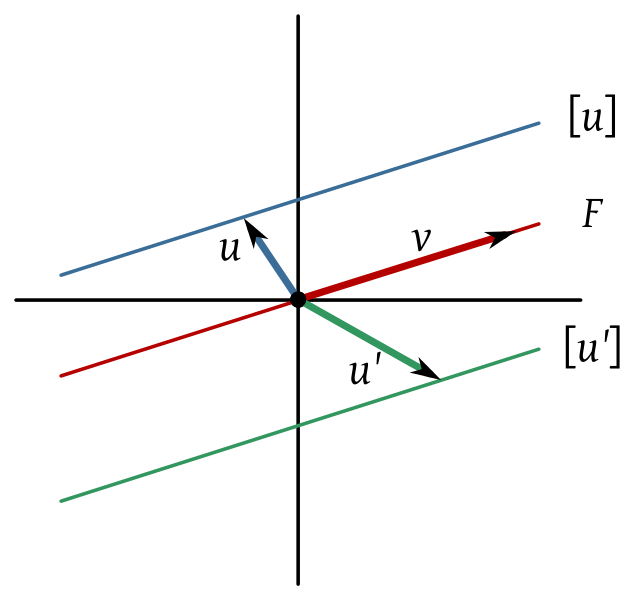
\includegraphics[scale=0.25]{clase lateral}
\end{center}
\end{defi}

\begin{defi}[Conjunto Cociente]
Se define el \textbf{conjunto cociente} y se denota por $V/W = \{[v]_W: v\in V\}$ al conjunto de clases laterales resultantes de la relación de equivalencia generada por $W$ y forma un K-ESPACIO-VECTORIAL las siguientes propiedades:
\begin{itemize}
\item $\bar{v}+\bar{v'}=\overline{v+v'}$
\item $a\cdot \bar{v}=\overline{a\cdot v}$
\end{itemize}
\end{defi}

\begin{obs}
Es notable destacar los siguientes aspectos:
\begin{itemize}
\item $0_{V/W}=[0]_W$ y que $-\bar{v}=\overline{-v}$.
\item Hay que comprobar que la suma y el producto están bien definidos, es decir, que no dependen del representante escogido para operar:
	\begin{itemize}
	\item Sean $\overline{v}_1=\overline{v}_2$ representantes de una clase y $\overline{v'}_1=\overline{v'}_2$ otros de otra distinta, entonces:
$$\overline{v_1+v_1'}=\overline{v_2+v_2'}\Leftrightarrow (v_1+v_1')-(v_2+v_2')=0\Leftrightarrow \underbrace{(v_1-v_2)}_{\in W}+\underbrace{(v_1'+v_2')}_{\in W}\in W$$
	\item El producto se demuestra de forma análoga.
	\end{itemize}
\end{itemize}
\end{obs}

\begin{prop}
Sea $V$ un espacio vectorial y $W<V$ un subespacio vectorial del mismo. Si denotamos $\dim V=n$ y $\dim W=m$, entonces $\dim V/W=n-m$.

De hecho, si $B=\{v_1, \cdots , v_m\}$ es una base de $W$ y $B' = \{v_1, \cdots, v_m, v_{m+1}, \cdots, v_n\}$ es una ampliación suya para $V$, entonces $B'' = \{\bar{v_{m+1}, \cdots, \bar{v_{n}}}\}$ es base de $V/W$.
\end{prop}
\begin{demo}
Elegimos una base cualquiera de $W$: $B_W=\{w_1,\cdots,w_m\}$ y ampliamos esta base para V: $B=\{w_1,\cdots, w_m, v_{m+1}, \cdots, v_n\}$, es decir, hemos añadido $n-m$ vectores a la base de $B_W$ para ampliarla a $B$. Ahora probamos que $\{\overline{v}_{m+1},\cdots \overline{v}_n\}$ es base de $V/W$.

\begin{itemize}
\item Linealmente independiente:
$$a_{m+1}\overline{v}_{m+1}+\cdots +a_n\overline{v}_n=0\Leftrightarrow \overline{a_{m+1}v_{m+1}+\cdots +a_nv_n}=0\Leftrightarrow a_{m+1}v_{m+1}+\cdots +a_nv_n- 0\in W$$
Como estos vectores pertenecen a $W$, entonces se podrán expresar en función de su base:
$$a_{m+1}v_{m+1}+\cdots +a_nv_n=a_1w_1+\cdots a_mw_m\Rightarrow a_{m+1}v_{m+1}+\cdots +a_nv_n-a_1w_1+\cdots a_mw_m=0\stackrel{B\mbox{ es base}}{\Rightarrow}\mbox{ l. ind.}$$

\item Sistema de generadores:
$$\forall v\in V: \overline{v}=\overline{a_1w_1+\cdots+a_mw_m+a_{m+1}v_{m+1}+\cdots+ a_nv_n}=\overline{a_1w_1+\cdots a_mw_m}+a_{m+1}\overline{v}_{m+1}+\cdots a_n\overline{v}_n=$$
Como $a_1w_1+\cdots a_mw_m\in W\Rightarrow \overline{a_1w_1+\cdots a_mw_m}=0$, luego tenemos que:
$$=a_{m+1}\overline{v}_{m+1}+\cdots a_n\overline{v}_n$$
Luego queda demostrado que para cualquier $\bar{v}$, este se puede expresar como combinación lineal de los vectores añadidos para ampliar la base, luego es sistema de generadores.
\end{itemize}
\end{demo}

\begin{ej}
En $\mathbb R^5$ consideramos $W$ como el subespacio\footnote{Más adelante se demostrará que esto es un subespacio} de los vectores cuyas coordenadas se ajustan al siguiente sistema: $W=\begin{cases}
x_1+x_2-x_5=0 \\
2x_1-x_4=0
\end{cases}$, vamos a ver que $\dim W=3$ y vamos a calcular la base de $B_{V/W}$.

Podemos ver que el sistema de ecuaciones forma un subespacio vectorial de V por ser un sistema homogéneo del que son vectores los vectores solución de ese sistema. Su dimensión es el número de incógnitas menos el rango de la matriz de coeficientes, es decir, $\dim W=5-2=3$. Esto es así porque según vimos en Bachillerato, es necesario que haya 3 incógnitas parametrizadas que en este caso van a ser $x_3, x_4, x_5$ y las otras toman valores conforme a ellas, así que esencialmente los vectores de $W$ dependen de 3 valores, de ahí la dimensión 3.

Para hallar los vectores de la base de $W$, vemos que la solución del sistema es: $(x_1,x_2,x_3,x_4,x_5)=(\frac{x_4}{2}, x_5-\frac{x_4}{2},x_3,x_4,x_5)$. Por lo que cualquier vector solución se puede escribir como:
$$x_3(0,0,1,0,0)+x_4(1,-1,0,1,0)+x_5(0,1,0,0,1)$$
Otra forma es dar valores de vectores que sean linealmente independientes entre los tres parámetros, p. ej., $(x_3,x_4,x_5)=(1,0,0),(0,1,0), (0,0,1)$ y hallar los valores de $x_1$ y $x_2$ para completar con las dos variables que faltan cada uno de los vectores.\par
Con lo cual, para encontrar la base ahora de $V/W$, vemos que  vectores es necesario añadir a la hallada para que sea base de $V$, un caso sencillo para ampliar la base es añadir vectores de la base canónica de $\mathbb R^5$:
$$B=\{(0,0,1,0,0),(1,-1,0,1,0),(0,1,0,0,1), v_1, v_2\}=$$
$$=\{(0,0,1,0,0),(1,-1,0,1,0),(0,1,0,0,1), e_1=(1,0,0,0,0), e_2=(0,1,0,0,0)\}$$
Con lo cual, $e_1$ y $e_2$ forman la base de $V/W$.
\end{ej}

\section{Aplicaciones Lineales}
Al inicio del capítulo comentamos que íbamos a ver las características la estructura de espacio vectorial, pero que también íbamos a ver las características de los morfismos entre estructuras de este tipo.

Por ello, esta sección está dedicada al estudio de las propiedades que tienen estas transformaciones: las aplicaciones lineales. Es muy común y habitual en matemáticas tener que definir o utilizar aplicaciones (funciones) entre objetos matemáticos. Si además añadimos que hemos comentado que la estructura de espacio vectorial está muy presente en multitud de elementos en las matemáticas, con más razón será necesario sacar provecho y ventajas de todas las propiedades que podamos descubrir de las mismas.

\begin{defi}
Sea $\phi:V\longrightarrow V'$ una aplicación entre dos espacios vectoriales, decimos que $\phi$ es una \textbf{aplicación lineal} si y sólo si conserva la suma y el producto por un escalar, es decir, si verifica que:
\begin{itemize}
\item $ \forall v_1,v_2\in V : \phi(v_1+v_2)=\phi(v_1)+\phi(v_2)$
\item $\forall a\in K,\ \forall v\in V : \phi(a\cdot v_1)=a\cdot \phi(v_1)$
\end{itemize}
Al conjunto de aplicaciones lineales entre ambos espacios se le denota\footnote{Si el espacio de llegada y de salida son el mismo, es decir, $V=V'$, entonces se denota por $End(V)$} por $Hom(V,V')$, de \textit{homomorfismos} de $V$ en $V'$.
\end{defi}

\begin{ej}
\begin{itemize}
\item Sea $\phi: K^3\longrightarrow K^2$ y $\phi(x,y,z)=(x-y, x+y+z)$:
$$\phi\left[(x,y,z)+(x',y',z')\right]=\phi(x+x',y+y',z+z')=(x+x'-y-y', x+x'+y+y'+z+z')=$$
$$=(x-y, x+y+z)+(x'+y',x'+y'+z')=\phi(x,y,z)+\phi(x',y',z')$$

\item Sea $\phi: V\longrightarrow V$ y sea $\phi$ $K-lineal$, entonces decimos que es un endomorfismo. Por ejemplo, $\phi: V\longrightarrow V$ siendo $id_V=\phi(v)=v$, es un endomorfismo.

\item Sea $\phi: V\longrightarrow V$ y sea $\phi(v)=r\cdot v$ donde $r\in K$, también es un isomorfismo. Concretamente a esto se le conoce como \textbf{homotecia}\footnote{Y en este caso además es un isomorfismo dentro del propio V}. $\phi$ cumple que $\phi=\phi^{-1}$ con lo que es fácil demostrar que es una biyección y por extensión un isomorfismo. 

\item Si tenemos $W<V$, podemos definir $V/W$ y ahora $\phi: V\longrightarrow V/W$ siendo $\phi(v)=\bar{v}$, entonces $\phi$ es aplicación lineal.

\item Si tenemos que $V=W\oplus U$ y $\phi: V\longrightarrow V$, entonces $v=w+u$ de modo único y la aplicación $\phi(v)=w$ es lineal. A esta aplicación se la conoce como \textbf{proyección} de $v$ con base $W$ y dirección $U$.
\begin{itemize}
\item Vamos a ver que ocurre con los vectores de $W$:
$$v\in W\Leftrightarrow \phi(v)=v$$

Esto es así porque:
$$v\in W\Rightarrow v=\underbrace{v}_{\in W}+\underbrace{0}_{\in U}\Rightarrow \phi(v)=v$$
$$\phi(v)=v\Rightarrow v=\underbrace{w}_{=v}+u\Rightarrow u=0\Rightarrow v\in W$$

\item Vamos a ver que ocurre con los vectores de $U$:
$$v\in U\Leftrightarrow \phi(v)=0$$

Esto es así porque:
$$v\in U\Rightarrow v=\underbrace{0}_{\in W}+\underbrace{v}_{\in U}\Rightarrow \phi(v)=0$$
$$\phi(v)=0\Rightarrow v=\underbrace{w}_{=0}+u\in U$$
\end{itemize}

\item Si tenemos que $V=W\oplus U$, entonces $v=w+u$ de modo único y la aplicación $\phi(v)=w-u$ es lineal. A esta aplicación se la conoce como \textbf{simetría} de $v$ con base $W$ y dirección $U$.
\begin{itemize}
\item Vamos a ver que ocurre con los vectores de $W$:
$$v\in W\Leftrightarrow \phi(v)=v$$

Esto es así porque:
$$v\in W\Rightarrow v=\underbrace{v}_{\in W}+\underbrace{0}_{\in U}\Rightarrow \phi(v)=v-0=v$$
$$\phi(v)=v\Rightarrow w-u=v=\underbrace{w}_{=v}+u\Rightarrow 2u=0\Rightarrow v=w\in W$$

\item Vamos a ver que ocurre con los vectores de $U$:
$$v\in U\Leftrightarrow \phi(v)=-v=-1_k\cdot v$$

Esto es así porque:
$$v\in U\Rightarrow v=\underbrace{0}_{\in W}+\underbrace{v}_{\in U}\Rightarrow \phi(v)=0-v=-v$$
$$\phi(v)=-v\Rightarrow w-u=-v=-w-u\Rightarrow 2w=0\Rightarrow v=u\in U$$
\end{itemize}
\end{itemize}
\end{ej}

\begin{defi}[Imagen y Núcleo]
Sea $\phi: V\longrightarrow V'$ una aplicación lineal, llamamos \textbf{imagen de $\phi$} al subespacio vectorial\footnote{La demostración de que es un subespacio vectorial del espacio de llegada es trivial por la condición de que las aplicaciones lineales conservan sumas y productos por escalares.} del espacio de llegada cuyos vectores son imagen de algún vector del espacio de salida:
$$
Im(\phi)=\{\phi(v): v\in V\}<V'
$$
Del mismo modo, llamamos \textbf{núcleo de $\phi$} al subespacio vectorial\footnotemark[7] del espacio de partida cuyos vectores se transforman en el vector nulo del espacio de llegada:
$$
\ker(\phi)=\{v\in V: \phi(v)=0_v\}<V
$$
\end{defi}

\begin{prop}
Sea $\phi: V\longrightarrow V'$ una aplicación lineal, entonces:
\begin{enumerate}
\item $\phi$ es suprayectiva $\Leftrightarrow Im(\phi)=V'$
\item $\phi$ es inyectiva $\Leftrightarrow \ker(\phi)=\{0_v\}$
\end{enumerate}
\end{prop}
\begin{demo}
\begin{enumerate}
\item trivial

\item De la primera se deduce que:
\begin{itemize}
\item ``$\Rightarrow$'': supongamos que es inyectiva\par
Vemos primero que: $\phi(0_v)=\phi(0_v+0_v)=\phi(0_v)+\phi(0_v)\Leftrightarrow 0_{v'}=\phi(0_v)\Rightarrow 0_v\in \ker(\phi)$, es decir, que el cero va al cero.
$$
v\in \ker(\phi)\Rightarrow \phi(v)=0_{v'}\Rightarrow \phi(v) = \phi(0)\Rightarrow \forall v\in \ker(\phi) : v=0
$$
por la inyectividad de $\phi$.

\item ``$\Leftarrow$'': supongamos cierto que el $\ker(\phi)=\{0_v\}$, entonces:
$$
\phi(v_1)=\phi(v_2)\Rightarrow \phi(v_1-v_2)=0_v'\Rightarrow v_1-v_2\in \ker(\phi)\Rightarrow v_1-v_2=0_v\Rightarrow v_1=v_2
$$
\end{itemize}
\end{enumerate}
\end{demo}

\begin{obs}
La demostración del enunciado anterior para la inyectividad pone de manifiesto que en las aplicaciones lineales SIEMPRE $\phi(0) = 0$.
\end{obs}

\textbf{Proyecciones}\par

Para las proyecciones resulta que la base es la imagen y la dirección es el núcleo de la misma, es decir, $Im(\phi)=W$ y $\ker(\phi)=U$, siendo $V=W\oplus U$. Además, en las proyecciones $\phi^2=\phi$.\par

\underline{Demostración}:
\begin{itemize}
\item $W=Im(\phi)$
\begin{itemize}

\item ``$\subset$'':
$$w\in W\Rightarrow w=w+0\Rightarrow \phi(w)=w\Rightarrow w\in Im(\phi)$$

\item ``$\supset$'':
$$w\in Im(\phi)\Rightarrow w=\phi(v)\Rightarrow \phi(v)\in W$$
\end{itemize}

\item $U=\ker(\phi)$:
$$v\in U\Leftrightarrow \phi(v)=0\Rightarrow v\in \ker(\phi)$$

\item $\phi \mbox{ proyección}\Leftrightarrow \phi^2=\phi$
\begin{itemize}
\item ``$\Rightarrow$'':
$$\phi^2(v)=\phi^2(w+u)=\phi(\phi(w+u))=\phi(w)=w=\phi(v)$$
Por ello se las llama idempotencias.

\item ``$\Leftarrow$'': tenemos que ser capaces de componer, sabiendo que $\phi^2=\phi$, que $V=W\oplus V$ siendo $W=\{v\in V: \phi(v)=v\}$ base de la simetría y $U=\{v\in V: \phi(v)=0\}$ dirección de la simetría. Es decir, partimos de la hipótesis y de la definición de ambos subespacios y hay que demostrar la suma directa.
$$v\in W\cap U\Leftrightarrow 0=\phi(v)=v\Leftrightarrow v=0\Rightarrow W\cap U=\{0\}$$
$$\phi(v)\in W\wedge v-\phi(v)\in U\Rightarrow v=\phi(v)+v-\phi(v)$$

Esto es así porque $\phi(\phi(v))=\phi^{2}(v)=\phi(v)\Rightarrow \in W$ y $\phi(v-\phi(v))=\phi(v)-\phi^2(v)=0\Rightarrow \in U$.

Solo falta ver que existe una proyección de $V$ con base $W$ y dirección $U$ que como es única, esta debe coincidir necesariamente con $\phi$:
$$\varphi: V\longrightarrow V\mbox{ proyección con base W y dirección U}\Rightarrow W=\{v\in V: \varphi(v)=v\}\wedge U=\{v\in V: \varphi(v)=0\}\Rightarrow$$
$$\Rightarrow v\in W \vee v\in U: \phi(v)=\varphi(v)\Rightarrow v\in V: v=w+u\Rightarrow \phi(v)=\phi(w)+\phi(u)=\varphi(w)+\varphi(u)=\varphi(v):\forall v\in V$$
\end{itemize}
\end{itemize}

Además, $\phi$ es suprayectiva:
$$\Leftrightarrow Im(\phi)=V\Leftrightarrow W=V \wedge U=\{0\}\Leftrightarrow id_v=\phi$$

Además, $\phi$ es inyectiva:
$$\Leftrightarrow \ker(\phi)=\{0\}\Leftrightarrow V=\{0\}\Leftrightarrow W=V\Leftrightarrow \phi=id_v$$

\textbf{Simetrías}\par

Para las simetrías resulta que $Im(\phi)=V$ y $\ker(\phi)=\{0\}$, por lo tanto todas las simetrías son inyectivas y suprayectivas y en consecuencia, isomorfismos. Además, en las simetrías $\phi=\phi^{-1}$.\par

\underline{Demostración}:
\begin{itemize}
\item $V=Im(\phi)$
$$v\in V\Leftrightarrow v=w+u \Rightarrow w-(-u)=\phi(w-u)\in Im(\phi)$$

\item $\{0\}=\ker(\phi)$:
$$v\in \ker(\phi)\wedge v=w+u\Rightarrow w+u=v=0=\phi(v)=w-u\Rightarrow u=w\Rightarrow u=w\in U\cap W=\{0\}\Rightarrow u=w=0=v$$

\item $\phi \mbox{ simetría}\Leftrightarrow \phi^{-1}=\phi$
\begin{itemize}
\item ``$\Rightarrow$'':
$$(\phi \circ \phi)(v)=\phi(\phi (v))=\phi(w-u)=w-(-u)=w+u=v\Rightarrow \phi=id_v$$
Por ello se las llama involuciones

\item ``$\Leftarrow$'': tenemos que ser capaces de componer, sabiendo que $\phi^2=id_V$, que $V=W\oplus V$ siendo $W=\{v\in V: \phi(v)=v\}$ base de la simetría y $U=\{v\in V: \phi(v)=-v\}$ dirección de la simetría. Es decir, partimos de la hipótesis y de la definición de ambos subespacios y hay que demostrar la suma directa.
$$v\in W\cap U\Leftrightarrow -v=\phi(v)=v\Leftrightarrow v=0\Rightarrow W\cap U=\{0\}$$
$$v+\phi(v)\in W\wedge v-\phi(v)\in U\Rightarrow v=\frac{v+\phi(v)}{2}+\frac{v-\phi(v)}{2}$$

Esto es así porque $\phi(v+\phi(v))=\phi(v)+v\Rightarrow \in W$ y $\phi(v-\phi(v))=\phi(v)-v\Rightarrow \in U$.

Solo falta ver que existe una simetría de $V$ con base $W$ y dirección $U$ que como es única, esta debe coincidir necesariamente con $\phi$:
$$\varphi: V\longrightarrow V\mbox{ simetría con base W y dirección U}\Rightarrow W=\{v\in V: \varphi(v)=v\}\wedge U=\{v\in V: \varphi(v)=-v\}\Rightarrow$$
$$\Rightarrow v\in W \vee v\in U: \phi(v)=\varphi(v)\Rightarrow v\in V: v=w+u\Rightarrow \phi(v)=\phi(w)+\phi(u)=\varphi(w)+\varphi(u)=\varphi(v):\forall v\in V$$
\end{itemize}
Por último, la relación que existe, dada la misma base y la misma dirección, entre las simetrías y las proyecciones es: $\mbox{Sean }\phi\mbox{ simetría y }\varphi \mbox{ la proyección asociada}$:
$$\begin{cases}\phi(v)=w-u \\ \varphi(v)=w \\ id(v)=w+u\end{cases}\Rightarrow (\phi+id)(v)=2w=2\varphi(v)\Rightarrow \frac{1}{2}\cdot (\phi + id)=\varphi$$
\end{itemize}

\begin{prop}[Operaciones con aplicaciones lineales]
Sean $\phi_1, \phi_2: V\longrightarrow V'$ aplicaciones $K-lineales$ y las operaciones:
\begin{itemize}
\item $(\phi_1+\phi_2)(v)\stackrel{def}{:=}\phi_1(v)+\phi_2(v)$
\item $(a\cdot \phi_1)(v)\stackrel{def}{:=}a\cdot \phi_1(v)$
\end{itemize}
entonces la terna $(Hom(V,V'),+,\cdot )$ tiene estructura de espacio vectorial.
\end{prop}

\begin{obs}
Del mismo modo, se puede ver que $(\phi_2 \circ \phi_1)(v)$ es también una aplicación lineal si ambas aplicaciones lo son. Con lo que $(End(V), +, \circ)$ conforma un anillo conmutativo y unitario.
\end{obs}

\begin{theo}
Sean $V$ y $V'$ espacios vectoriales, $B:=\{v_1, \cdots, v_n\}$ una base de $V$ y $v_1', \cdots, v_n'\in V'$ vectores arbitrarios de $V'$, entonces:
$$
\exists! \phi: V\longrightarrow V' \mbox{ tal que } \phi(v_i)=v_i': \forall i=1,\cdots,n
$$
es decir, una aplicación lineal queda únicamente determinada por la imagen de los vectores de una base del espacio de partida.
\end{theo}
\begin{demo}
\begin{itemize}
\item Existencia:

Cualquier $v=(a_1, \cdots, a_n)_B \in V$ se expresa en términos de la base $B$ como $v=\sum_{i=1}^n a_iv_i$, luego parece razonable que definamos la aplicación $\phi$ como $\phi(v) := \sum_{i=1}^na_iv_i'$. Para probar que efectivamente esta definición cumple el enunciado, no hay más que demostrar su linealidad:
$$
v+w = (a_1+b_1,\cdots, a_n+b_n)_B \Rightarrow \phi(v+w) = \sum_{i=1}^n (a_i+b_i)v_i' = \sum_{i=1}^na_iv_i' + \sum_{i=1}^nb_iv_i'=\phi(v)+\phi(w)
$$
$$
a\cdot v=(a\cdot a_1, \cdots, a\cdot a_n)_B\Rightarrow \phi(a\cdot v)=\sum_{i=1}^n(a\cdot a_i)v_i'=a\cdot \sum_{i=1}^na_iv_i'=a\cdot \phi(v)
$$
y que conserva la propiedad $\phi(v_i) = v_i'$ del enunciado:
$$
v_i=(0,\cdots,1,\cdots,0)_B\Rightarrow \phi(v_i)=1\cdot v_i'=v_i'
$$

\item Unicidad:

Supongamos que hay dos y veamos que son la misma. Como hay dos, sabemos que $\phi(v_i)=\varphi(v_i)=v_i'$, luego:
$$
\phi(v)=\phi\left(\sum_{i=1}^na_iv_i\right)=\sum_{i=1}^na_i\phi(v_i)=\sum_{i=1}^na_iv_i'
$$
$$
\varphi(v)=\varphi\left(\sum_{i=1}^na_iv_i\right)=\sum_{i=1}^na_i\varphi(v_i)=\sum_{i=1}^na_iv_i'
$$
\end{itemize}
\end{demo}

\begin{ej}
Sean $V=K^2$ y $V'=K^3$, solo hay una aplicación lineal que cumpla que
\begin{align*}
\phi(e_1)=(2,1,-3) & & \phi(e_2)=(0,1,0)
\end{align*}
porque como cada vector está definido en términos de la base, la aplicación es lineal y los vectores de la base tienen determinada su imagen, entonces para un vector arbitrario ocurre que:
$$
\phi(a_1, a_2)=\phi(a_1e_1+a_2e_2)=a_1(2,1,-3)+a_2(0,1,0)=(2a_1, a_1+a_2, -3a_1)
$$
\end{ej}

\subsection{Isomorfía de Espacios Vectoriales}
Ya hemos visto que en general si conozco las coordenadas de un vector conozco prácticamente todo lo relevante para los resultados que hemos expuesto sobre cambios de base y aplicaciones lineales. Como trabajar con el vector simplemente conociendo sus coordenadas es lo mismo que trabajar en $K^n$, esto nos da una pista sobre que trabajar en un espacio vectorial cualquiera va a ser muy parecido, si no igual, a trabajar en $K^n$.

Cuando dos espacios vectoriales tienen la misma estructura, se dice que son isomorfos. Esto tiene grandes ventajas pues por muy complicado que sea el espacio en el que me muevo, si conozco un espacio vectorial que sea isomorfo a él y donde me maneje bien, entonces podré trabajar indistintamente en este último y aplicar los resultados del mismo en el primero (a través de una biyección entre los espacios adecuada).

\begin{theo}
Dos espacios vectoriales son isomorfos si y solo si la dimensión de ambos es la misma.
$$V\simeq V'\Leftrightarrow \dim_k V=\dim_k V'$$
\end{theo}
\begin{demo}
\begin{itemize}
\item ``$\Rightarrow$'': vamos a ver que $B'=\{\phi(v_1), \cdots, \phi(v_n)\}$ es base de V'\par
Sea $B=\{v_1, \cdots, v_n\}$ base de $V$ y $\phi: V\longrightarrow V'$ un isomorfismo, entonces:
$$v'\in V\stackrel{isomf}{\Rightarrow} v'=\phi(v)=\phi(a_1v_1+\cdots+a_nv_n)=a_1\phi(v_1)+\cdots+a_n\phi(v_n)\Rightarrow \{\phi(v_1), \cdots, \phi(v_n)\}\mbox{ es sist. gener.}$$
Ahora vemos que son linealmente independientes:
$$0=a_1\phi(v_1)+\cdots+a_n\phi(v_n)=\phi(a_1v_1+\cdots+a_nv_n)\Rightarrow a_1v_1+\cdots+a_nv_n\in \ker(\phi)=\{0\}\Rightarrow 0=a_1v_1+\cdots+a_nv_n=0$$

\item ``$\Leftarrow$'':\par
Sea $B=\{v_1, \cdots, v_n\}$ base de $V$ y $B'=\{v_1', \cdots, v_n'\}$ base de $V'$, entonces:
$$\exists! \phi: V\longrightarrow V': \phi(v_i)=v_i': \forall i=1,\cdots, n$$
$$\exists! \varphi: V'\longrightarrow V: \varphi(v_i')=v_i: \forall i=1,\cdots, n$$
$$\varphi \circ \phi: V\longrightarrow V\Rightarrow (\varphi \circ \phi)(v_i)=\varphi(v_i')=v_i\Rightarrow \varphi \circ \phi=id_V$$
Pero del mismo modo se sigue que:
$$\phi \circ \varphi: V\longrightarrow V\Rightarrow (\phi \circ \varphi)(v_i)=\phi(v_i')=v_i\Rightarrow \phi \circ \varphi=id_{V'}$$
Lo que implica que ambas son biyectivas y como son lineales, ambas son isomorfismos.
\end{itemize}
\end{demo}

\begin{coro}
Si la dimensión de un espacio cualquiera es $n$, entonces es isomorfo al producto cartesiano de $n$ veces $K$.
$$\dim_k V=n\Rightarrow V\simeq K^n$$
\end{coro}
\begin{demo}
$$\dim_k V=n=\dim_k K^n\Rightarrow V\simeq K^n$$
Sin embargo, no podemos identificar un isomorfismo canónico que verifique este teorema, solo podemos afirmar que existe porque para poder identificarlo es necesario definir una base de $V'$ y cambia en función de la base elegida.
\end{demo}

\begin{theo}[de la dimensión]
Sea $\phi: V\longrightarrow V'$ una aplicación lineal y $V$ un espacio vectorial con dimensión finita $\dim_k V=n$, entonces se cumple que:
\begin{enumerate}
\item $\ker(\phi)$ y $Im(\phi)$ son de dimensión finita.
\item $\dim_k \ker(\phi)+\dim_k Im(\phi)=n$
\end{enumerate}
\end{theo}
\begin{demo}
Como $\ker(\phi)<V$ y $\dim_k V=n$ entonces sabemos que $\dim_k \ker(\phi)\leq n$, por tanto, escogemos una base del $\ker (\phi)$ como $\{v_{r+1}, \cdots, v_{n}\}$ y la extendemos a $V$ de modo que la base de V es $B=\{v_1,\cdots , v_r, v_{r+1}, \cdots , v_n\}$ con estos últimos $n-r$ vectores del $\ker (\phi)$.

Vamos a ver que $\{\phi(v_1), \cdots, \phi(v_r)\}$ es una base de la $Im(\phi)$:
$$v'\in Im(\phi)\Rightarrow v'=\phi(v)=\phi(a_1v_1+\cdots+a_rv_r+a_{r+1}v_{r+1}+\cdots+a_nv_n)=$$
$$=a_1\phi(v_1)+\cdots+a_r\phi(v_r)+a_{r+1}v_{r+1}+\cdots+a_n\phi(v_n)=a_1\phi(v_1)+\cdots+a_r\phi(v_r)$$

Y ahora vemos que estos son linealmente independientes:
$$0=a_1\phi(v_1)+\cdots+a_r\phi(v_r)=\phi(a_1v_1+\cdots+a_rv_r)\Rightarrow a_1v_1+\cdots+a_rv_r\in \ker(\phi)\Rightarrow a_1v_1+\cdots+a_rv_r=$$
$$=a_{r+1}v_{r+1}+\cdots+a_nv_n\Leftrightarrow a_1v_1+\cdots+a_rv_r-a_{r+1}v_{r+1}-\cdots-a_nv_n=0\Rightarrow a_1=\cdots=a_r=a_{r+1}=\cdots=a_n=0$$
\end{demo}

\begin{theo}[Primer Teorema de Isomorfía]
Supongamos que $\phi: V\longrightarrow V'$ es una aplicación K-lineal se cumple que:
$$V/\ker(\phi)\simeq Im(\phi)$$
Este teorema vale siempre, sea cual sea la dimensión de V
\end{theo}
\begin{demo}
Supongamos que $V$ es de dimensión finita, entonces $\ker(\phi)$ y $Im(\phi)$ también son finitos por el teorema de la dimensión, además sabemos que:
$$\dim V= \dim \ker(\phi)+ \dim Im(\phi)\Leftrightarrow \dim V- \dim \ker(\phi)=\dim Im(\phi)\Leftrightarrow \dim V/\ker(\phi)=\dim Im(\phi)$$
$$\Rightarrow V/\ker(\phi)\simeq Im(\phi)$$
Vamos ahora a ver la aplicación lineal que relaciona ambos conjuntos y establece el isomorfismo:
$$\bar{\phi}: V/\ker(\phi) \longrightarrow Im(\phi)$$
$$\overline{\phi}(\bar{v})=\phi(v)$$
De este modo ya se cumple el isomorfismo, pero hay que comprobar que está bien definida probando que:
$$\bar{v}=\bar{w}\Rightarrow \phi(v)=\phi(w)$$
Y por último también que:
$$\phi \mbox{ es lineal, inyectiva y suprayectiva}$$
\end{demo}

\begin{theo}[Segundo Teorema de Isomorfía]
Consideramos $W, U<V$ y definimos los subespacios:
$$(W+U)/W\simeq U/(W\cap U)$$
\end{theo}
\begin{demo}
Considerando $W$ y $U$ de dimensión finita, entonces $W+U$ es de dimensión finita y $W\cap U$ también lo es. Ahora vemos que:
$$\dim (W+U/W)=\dim (W+U)- \dim W\stackrel{Grassman}{=}\dim U-\dim (W\cap U)=\dim (U/W\cap U)$$
\end{demo}

\subsection{Matriz asociada a una aplicación lineal}
El hecho de que una aplicación lineal quede determinada de modo único por su imagen a través de los vectores de una base sugiere que la información necesaria para conocer a una aplicación lineal es finita. Por tanto, existirá una representación de la misma que contenga esta información finita y que simplifique la forma de trabajar con ella.

Sea $\phi: V\longrightarrow V'$ una aplicación K-lineal, $B=\{v_1,\cdots, v_n\}$ una base de $V$ y $B'=\{v_1',\cdots, v_m'\}$ una de $V'$, sabemos que $\phi$ está determinada de modo único por su imagen a través de los vectores de la base $B$:
$$
\begin{cases}\phi(v_1)=a_{11}v_1'+\cdots+a_{m1}v_m'
\\ \vdots \\ \phi(v_n)=a_{1n}v_1'+\cdots+a_{mn}v_m'\end{cases}
$$
Por otro lado, si calculamos la imagen de un vector $v$ arbitrario tenemos que:
\begin{eqnarray*}
\phi(v)
&=& \phi(x_1v_1+\cdots+x_nv_n) \\
&=& x_1\phi(v_1)+\cdots+x_n\phi(v_n) \\
&=& x_1(a_{11}v_1'+\cdots+a_{m1}v_m')+ \cdots + x_n(a_{1n}v_1'+\cdots + a_{mn}v_m') \\
&=& \underbrace{(a_{11}x_1+\cdots+a_{1n}x_n)}_{x_1'}v_1'+\cdots\underbrace{(a_{m1}x_1+\cdots+a_{mn}x_n)}_{x_m'}v_m'
\end{eqnarray*}
Por tanto, podemos observar que la relación con las coordenadas $(x_1', \cdots, x_m')$ se puede ver como un sistema lineal en el que interviene la información sobre la imagen de los vectores de la base inicial. Dicho sistema lineal, si se representa en su expresión matricial, tiene la forma:
Con lo cual para transformar un vector en otro tenemos que:
$$\left(\begin{array}{c} \overbrace{x_1'}^{\phi(v)} \\ \vdots\\ x_m'\end{array}\right)=\underbrace{\left(\begin{array}{ccc} \overbrace{a_{11}}^{\phi(v_1)} & \cdots & \overbrace{a_{1n}}^{\phi(v_n)} \\ \vdots & \ddots & \vdots \\ a_{m1} & \cdots & a_{mn} \end{array}\right)}_{M_{B,B'}(\phi)}\cdot \left(\begin{array}{c} \overbrace{x_1}^{v} \\ \vdots\\ x_n\end{array}\right) \Rightarrow \phi(v) = M_{B,B'}(\phi)\cdot v^t$$

\begin{theo}[de la Matriz Asociada]
Sea $\phi: V\longrightarrow V'$ una aplicación K-lineal, $B=\{v_1,\cdots, v_n\}$ una base de $V$ y $B'=\{v_1',\cdots, v_m'\}$ una de $V'$, podemos expresar la aplicación lineal como:
$$
\forall v\in V : \phi(v) = M_{B,B'}(\phi) \cdot v^t
$$
\end{theo}

\begin{prop}[Operaciones con matrices asociadas]
\begin{itemize}
\item Sean $\phi_1,\phi_2 : V\longrightarrow V'$ dos aplicaciones lineales y $B$ y $B'$ bases respectivas de los espacios $V$ y $V'$, entonces:
$$
M_{B,B'}(\phi_1+\phi_2)=M_{B,B'}(\phi_1)+M_{B,B'}(\phi_2)
$$

\item Sea $\phi : V\longrightarrow V'$, $B$ y $B'$ bases respectivas y $a\in \mathbb K$, entonces:
$$
M_{B,B'}(a\cdot \phi)=a \cdot M_{B,B'}(\phi)
$$

\item Sean las aplicaciones $V\stackrel{\phi}{\longrightarrow} V'\stackrel{\varphi}{\longrightarrow } V''$ y $B$ y $B'$ bases respectivas, entonces:
$$
M_{B,B''}(\varphi\circ \phi)=M_{B',B''}(\varphi)\cdot M_{B,B'}(\phi)
$$
\end{itemize}
\end{prop}

\begin{prop}
Sea $(Hom_k(V,V'), +, \cdot )$ el espacio vectorial de los homomorfismos de $V'$ en $V$ y suponiendo $\dim V=n$ y $\dim V'=m$, entonces
\begin{eqnarray*} \Phi:(V,V') &\longrightarrow& Mat_{m\times n}(K)\\ \phi &\longmapsto& M_{B,B'}(\phi) 
\end{eqnarray*} 
es un isomorfismo de espacios vectoriales, es decir:
$$
Hom_k(V,V')\simeq Mat_{m\times n}(K)
$$
\end{prop}
\begin{demo}
\begin{itemize}
\item Está bien definida porque ya comprobamos que toda aplicación lineal está definida de módo único por la transformación de los vectores de una base y además cada aplicación podía escribirse en forma de matriz, que está asociada a cada $\phi$.

\item La suma y el producto se respetan de forma trivial.

\item Que es inyectiva:
$$\phi\in \ker(\phi)\Rightarrow \Phi(\phi)=0\Rightarrow \Phi(\phi)=Mat_{B,B'}(\phi)\Rightarrow \phi(v_1)=\cdots=\phi(v_n)=0\Rightarrow \phi=0\Rightarrow Inyectiva$$

\item Ahora que es suprayectiva:
$$A=\begin{pmatrix}
a_{11} & \cdots & a_{1n} \\ \vdots & \ddots & \vdots \\ a_{m1} & \cdots & a_{mn}\end{pmatrix}\in Mat_{m\times n}(K)\Rightarrow \exists \phi: V\rightarrow V'\mbox{ tal que }\phi(v_i)=a_{1i}v_1'+\cdots+a_{mi}v_m'\Rightarrow \exists!\phi\Rightarrow Sobre$$

Como para que la imagen de $\phi$ sea $A$ tiene que definirse a partir de los vectores de V', entonces es única porque ya demostramos que estos la determinan.
\end{itemize}
\end{demo}

\begin{obs}
Como el resultado anterior es cierto para cualesquiera $V$ y $V'$, entonces $End_k(V)\simeq Mat_n(K)$ a través del mismo isomorfismo.
\end{obs}

\subsubsection{Equivalencia de aplicaciones lineales y relación entre sus matrices}
Después de identificar cada aplicación lineal con su matriz asociada, puede surgir la siguiente pregunta: ¿cómo cambia la matriz si cambio las bases respecto de las cuales está definida $\phi$?

Además, si la matriz asociada cambia al elegir bases distintas, tiene sentido definir un conjunto cociente donde las matrices que representan a la misma aplicación lineal desde bases distintas sean todas equivalentes.

\begin{defi}[Equivalencia de matrices]
Sea $A_1, A_2\in Mat_{m\times n}(K)$ y $V, V'$ espacios vectoriales de dimensiones $n$ y $m$ respectivamente, decimos que son \textbf{matrices equivalentes} si y sólo si:
$$A_1\approx A_2 \Leftrightarrow \exists \phi: V\rightarrow V'\mbox{ lineal y bases } B_1,B_2\subset V \mbox{ y } B_1', B_2'\subset V': \begin{cases}
A_1=M_{B_1,B_1'}(\phi) \\ A_2=M_{B_2,B_2'}(\phi)
\end{cases}$$
es decir, si representan a la misma aplicación lineal respecto de bases distintas.
\end{defi}

Por tanto, el estudio de este conjunto cociente ahora se debería centrar en ver si cada clase de equivalencia tiene más de un elemento y ver cómo se relacionan los elementos de la misma clase de equivalencia. Para ello, supongamos una aplicación $\phi: V\longrightarrow V'$ y $B_1, B_2$ bases de $V$ y $B_1', B_2'$ bases de $V'$, con matrices\footnote{Nótese que pueden considerarse ambas matrices como matrices de una aplicación lineal porque anteriormente hemos demostrado que existía un isomorfismo entre el conjunto de matrices y el de aplicaciones.} asociadas:
\begin{align*}
A_1=Mat_{B_1,B_1'}(\phi) & & A_2=Mat_{B_2,B_2'}{}(\phi)
\end{align*}
A través del siguiente diagrama, se puede ver que considerar la aplicación expresada en términos de $B_1$ y $B_1'$ es lo mismo que considerarla en términos de $B_2$ y $B_2'$ pero cambiando de base antes y después para que todo se exprese en las bases iniciales:
$$
\underbrace{V}_{B_1}\xrightarrow{id_v} \underbrace{V}_{B_2} \xrightarrow{\phi} \underbrace{V'}_{B'_2} \xrightarrow{id_{v'}} \underbrace{V'}_{B'_1}
$$
es decir, que podemos ver $M_{B_1,B_1'}(\phi) = A_1$ como la composición\footnote{Nótese que la composición de funciones se hace en orden inverso al producto de las mismas.} de las funciones que en el diagrama anterior aparecen, luego:
$$
A_1=M_{B_1,B_1'}(\phi)=M_{B_2',B_1'}(id_{V'})\cdot M_{B_2,B_2'}(\phi)\cdot M_{B_1, B_2}(id_V)=\underbrace{M(B_2',B_1')}_{Q}\cdot A_2\cdot \underbrace{M(B_1,B_2)}_{P}=Q\cdot A_2\cdot P
$$
Como $P$ y $Q$ son matrices de cambio de base, pertenecen al grupo lineal, es decir, tienen inversa. Esto permite expresar, simplemente multiplicando por la inversa en ambos lados, $A_2$ en término de $A_1$ por matrices cuadradas del mismo modo que lo estábamos haciendo para $A_1$. Con este último resultado estamos en condiciones de poder reformular la definición de equivalencia de matrices de la siguiente manera.

\begin{defi}[Equivalencia de matrices]
Sean $A_1, A_2\in Mat_{m\times n}(K)$, se define la \textbf{equivalencia} como:
$$A_1\approx A_2 \Leftrightarrow \exists P\in GL_n(K), Q\in GL_m(K) :  A_1=Q\cdot A_2\cdot P$$
donde el conjunto $GL(K)$ se refiere a las matrices inversibles de los tamaños adecuados.
\end{defi}

\begin{obs}
El desarrollo anterior permite relacionar todas las matrices que expresan a una aplicación lineal a través de una clase de equivalencia en el conjunto cociente que induce la relación de equivalencia entre matrices.
\end{obs}

\begin{prop}
Sea $V$ un espacio vectorial, $B = \{v_1, \cdots, v_n\}$ una base del mismo y $P\in Gl_n(K)$ de  la forma $P=(p_{ij})$, entonces el conjunto de vectores:
$$
B' := \left\lbrace v_1'=\sum_{i=1}^np_{i1}v_i, \cdots , v_n'=\sum_{i=1}^n p_{in}v_i\right\rbrace
$$
es base de $V$ y $P$ es la matriz de cambio de base a $B'$.
\end{prop}
\begin{demo}
\begin{enumerate}
\item Veamos la independencia lineal, pues como hay tantos vectores como dimensión del espacio, se cumpliría trivialmente que es base
\begin{eqnarray*}
0
&=& a_1v_1'+\cdots+ a_nv_n' \\
&=& a_1(p_{11}v_1+\cdots p_{n1}v_n)+\cdots +a_n(p_{1n}v_1+\cdots p_{nm}v_n) \\
&=& (p_{11}a_1+\cdots p_{1n}a_n)v_1+\cdots +(p_{n1}a_1+\cdots +p_{nm}a_n)v_n
\end{eqnarray*}
Como los vectores $v_i$ formaban una base, los coeficientes asociados a cada uno en la expresión anterior son nulos. Esto, expresado de forma matricial, se puede escribir como:
$$
\begin{cases}
p_{11}a_1+\cdots p_{1n}a_n=0 \\
\vdots \\
p_{n1}a_1+\cdots +p_{nm}a_n
\end{cases}\Rightarrow P\cdot \begin{pmatrix} a_1 \\ \vdots \\ a_n\end{pmatrix}= \begin{pmatrix} 0 \\ \vdots \\ 0\end{pmatrix}\Leftrightarrow   \begin{pmatrix} a_1 \\ \vdots \\ a_n\end{pmatrix}= P^{-1}\cdot \begin{pmatrix} 0 \\ \vdots \\ 0\end{pmatrix}=0\Rightarrow  a_i=0 $$

\item Probado lo anterior, esto es trivial pues si lo primero es cierto, coger cada vector de $B'$ y expresarlo en base $B$, hace que los coeficientes de $P$ sean sus coordenadas.
\end{enumerate}
\end{demo}

\begin{obs}
Del mismo modo que pudimos identificar cada matriz con una aplicación lineal de la que es asociada, el teorema anterior nos permite considerar que toda matriz inversible es una matriz de algún cambio de base dentro de un espacio vectorial.
\end{obs}

\subsection{Rango de una aplicación lineal}
Una característica fundamental tanto de las aplicaciones lineales como del álgebra matricial es el rango de dicho objeto. Esta característica nos permite desde discutir sistemas lineales para elucubrar sus posibles soluciones como conocer la dimensión de la imagen del subespacio de llegada de una aplicación lineal.

\begin{defi}[Rango de una aplicación]
Sea $\phi: V\rightarrow V'$ una aplicación lineal, definimos el \textbf{rango de la aplicación} como:
$$
rg(\phi) := \dim_k Im(\phi)
$$
es decir, es la dimensión del subespacio imagen de la aplicación lineal.
\end{defi}

Si consideramos una matriz $A\in Mat_{m\times n}(K)$ definida como $A=(a_{ij})$, vimos que esta se podía interpretar como la matriz asociada a una aplicación lineal y, en ese caso, el rango de la aplicación lineal se correspondería con la dimensión de la envoltura lineal de los vectores columna (imagen de los de la base) que definen la imagen de la aplicación lineal. Por esto, tiene sentido dar la siguiente definición.

\begin{defi}[Rango de una matriz]
Sea $A\in Mat_{m\times n}(K)$ una matriz definida como $A=(a_{ij})$, definimos el \textbf{rango de la matriz} como: 
$$
rg(A) := \dim_k L(a_{11}e_{1}+\cdots+a_{m1}e_m, \cdots , a_{1n}e_1+\cdots+a_{mn}e_m)
$$
es decir, $rg(A)$ es la dimensión del subespacio generado por los vectores columnas de la matriz $A$.
\end{defi}

\begin{obs}
Como la dimensión de la envoltura lineal es el número de vectores linealmente independientes, esto nos proporciona un método para calcular la dimensión de un subespacio o la independencia lineal de un conjunto de vectores.
\end{obs}

Claramente la definición anterior que se ha dado para el rango de una matriz solo es interesante si dicho rango se conserva entre todas las matrices que pueden representar una misma aplicación lineal. Por tanto, nuestros pasos se encaminan a poder decir que dicho rango depende exclusivamente de la aplicación lineal y no de la representación escogida para la misma.

\begin{lema}
Sea $A=(a_{ij})\in Mat_{m\times n}(K)$ y $W$ a un espacio vectorial cualquiera de dimensión $\dim W=m$ escogemos una base suya $B=\{w_1, \cdots, w_m\}$ y la definición de rango de la matriz $A$ no cambia.
$$rg(A)=\dim L(a_{11}w_{1}+\cdots+a_{m1}w_m, \cdots, a_{1n}w_1+\cdots+a_{mn}w_m)$$
\end{lema}
\begin{demo}
En el fondo, la dimensión de $L()$ no es más que el número de vectores linealmente independientes de ese sistema de generadores, por lo que yo si encuentro un conjunto de vectores linealmente independientes maximal de los que forman ese sistema, entonces serán una base. Por ello podemos considerar que hay una cantidad $p\leq n$ de vectores linealmente independientes siendo $n$ el número de vectores que hay dentro de $L()$.  Y lo mismo ocurre con el $L()$ de la condición 2) del rango de una aplicación lineal, en el que designaremos su $p$ por $q$. Ahora se trata de ver que $p=q$
$$\{a_{11}e_{1}+\cdots+a_{m1}e_m, \cdots, a_{1q}e_1+\cdots+a_{mq}e_m\}\mbox{ supongamoslos l. ind.}$$
Tenemos que llegar a que $\{a_{11}w_1+\cdots+a_{m1}w_m,\cdots,a_{1q}w_1+\cdots+a_{mq}w_m\}$ son linealmente independientes.
$$0=\lambda_1(a_{11}w_1+\cdots+a_{m1}w_m)+\cdots+\lambda_q(a_{1q}w_1+\cdots+a_{mq}w_m)=$$
$$=(\lambda_1a_{11}+\cdots+\lambda_qa_{1q})w_1+\cdots+(\lambda_1a_{m1}+\cdots+\lambda_qa_{mq})w_m\Rightarrow $$
Como $B=\{w_1, \cdots, w_m\}$ es base de $W$, entonces:
$$0=\underbrace{(\lambda_1a_{11}+\cdots+\lambda_qa_{1q})}_{=0}w_1+\cdots+\underbrace{(\lambda_1a_{m1}+\cdots+\lambda_qa_{mq})}_{=0}w_m\Rightarrow$$
$$\Rightarrow  0=(\lambda_1a_{11}+\cdots+\lambda_qa_{1q})e_1+\cdots+(\lambda_1a_{m1}+\cdots+\lambda_qa_{mq})e_m=$$
$$=\lambda_1(a_{11}e_1+\cdots+a_{m1}e_m)+\cdots+\lambda_q(a_{1q}e_1+\cdots+a_{mq}e_m)\Rightarrow \lambda_1=\cdots=\lambda_q=0$$
Porque $B=\{e_1, \cdots, e_m \}$ es base.
\end{demo}

\begin{obs}
Este lema lo que nos resume es que para la definición del rango de una matriz, se pueden utilizar los vectores de la base de un espacio de dimensión $m$ cualquiera, es decir, que no es necesario que sean los del espacio $K^m$ ni tampoco los de la base canónica de un espacio.
\end{obs}

\begin{prop}
Sea $\phi: V\rightarrow V'$ una aplicación lineal y $A = M_{B,B'}(\phi)$ su representación matricial en bases arbitrarias, entonces:
$$
\forall A = M_{B,B'}(\phi) \in  Mat_{m\times n}(K) :  rg(\phi)=rg(A)
$$
es decir, el rango de la aplicación y de la matriz coincide para todas las matrices equivalentes.
\end{prop}
\begin{demo}
Simplemente basta con ver que
$$
rg(\phi)=\dim Im(\phi)=\dim L(\phi(v_1), \cdots, \phi(v_n))=\dim L(a_{11}v_1'+\cdots + a_{m1}v_m', \cdots , a_{1n}v_1'+\cdots +a_{mn}v_m')
$$
y precisamente el lema anterior nos dice que este último término es igual al rango de $A$.
\end{demo}

\begin{prop}
Sea $A\in Mat_{m\times n}(K)$ con rango $r$, entonces $A$ es equivalente a una matriz\footnote{Esta notación quiere decir que la matriz se puede dividir en 4 cuadrantes desiguales, la parte superior izquierda corresponde a una matriz identidad cuadrada de tamaño $r$ y el resto de cuadrantes a matrices nulas que no tienen por qué ser cuadradas.} con esta forma:
$$
A\approx A'=\left(\begin{array}{c|c} I_r & 0  \\ \hline 0 & 0 \end{array}\right) \in Mat_{m\times n}(K)
$$
\end{prop}
\begin{demo}
$$A=M_{B,B'}(\phi), \phi: \underbrace{V}_{B_1}\rightarrow \underbrace{V'}_{B_1'}$$
Ahora definimos $B_2=\{w_1,\cdots, w_r, \underbrace{w_{r+1}, \cdots, w_n}_{B\mbox{ del }\ker(\phi)}\}$ base de $V$ y esto puede hacerse por el teorema de la dimensión. Y $B'_2=\{\phi(w_1'),\cdots, \phi(w_{r}'), w_{r+1}', \cdots ,w_m'\}$ base de $V'$, es decir, los primeros son imágenes de los primeros de $B_1'$ y después se amplía la base hasta $V'$, pero para ello primero hay que comprobar que las imágenes son linealmente independientes.
$$0=a_1\phi(w_1)+\cdots+ a_r\phi(w_r)=\phi(a_1w_1+\cdots+a_rw_r)=\phi(a_1w_1+\cdots+a_rw_r)\Rightarrow v=a_1w_1+\cdots+a_rw_r\in \ker(\phi)\Rightarrow$$
$$\Rightarrow v=a_{r+1}w_{r+1}+\cdots+a_nw_n\Rightarrow a_1w_1+\cdots+a_rw_r=a_{r+1}w_{r+1}+\cdots+a_nw_n\Leftrightarrow$$
$$\Leftrightarrow a_1w_1+\cdots+a_rw_r-a_{r+1}w_{r+1}-\cdots-a_nw_n=0$$
Pero como son base: $a_1=\cdots=a_r=0\Rightarrow $ demostrado que son linealmente independientes.
Con lo cual, quien es esta matriz?:
$$Mat_{B_2, B_2'}(\phi)=\begin{pmatrix}
\overbrace{1}^{\phi(w_1)_{B_2'}} & \overbrace{0}^{\phi(w_2)_{B_2'}} & \overbrace{0}^{\cdots} & \cdots & \overbrace{0}^{\phi(w_r)_{B_2'}} & \overbrace{\cdots}^{\phi(w_{r+1}), \cdots=0} & \overbrace{0}^{\phi(w_n)=0} \\
0 & 1 & 0 & \cdots & 0 & \cdots & 0 \\
0 & 0 & 1 & \cdots & 0 & \cdots & 0 \\
\vdots & \vdots & \vdots & \ddots & 0 & \cdots & 0 \\
0 & 0 & 0 & \cdots & 1 & \cdots & 0 \\
\vdots & \vdots & \vdots & \vdots & \vdots & \cdots & 0 \\
0 & 0 & 0 & \cdots & 0 & \cdots & 0 \\
\end{pmatrix}$$
\end{demo}

\begin{prop}
Sean $A_1, A_2 \in Mat_{m\times n}(K)$, entonces:
$$
A_1\approx A_2\Leftrightarrow rg(A_1)=rg(A_2)
$$
es decir, la equivalencia se caracteriza por rangos.
\end{prop}
\begin{demo}
\begin{itemize}
\item ``$\Rightarrow $'':
$$
A_1=M_{B_1, B_1'}(\phi) \mbox{ y } A_2=M_{B_2, B_2'}(\phi) \Rightarrow rg(A_1)=rg(\phi)=rg(A_2)
$$

\item ``$\Leftarrow$'':
$$
rg(A_1)=rg(A_2)=r\Rightarrow A_1\approx \left(\begin{array}{c|c} I_r & 0  \\ \hline 0 & 0 \end{array}\right) \mbox{ y } A_2\approx\left(\begin{array}{c|c} I_r & 0  \\ \hline 0 & 0 \end{array}\right) \Rightarrow A_1\approx A_2
$$
\end{itemize}
\end{demo}

\begin{obs}
Los enunciados anteriores permiten, no solo caracterizar la relación de equivalencia entre matrices a través del rango, sino conocer el número de clases de equivalencia y el mejor representante de cada una en el conjunto cociente $Mat_{m\times n}(K)/\approx $. Por ejemplo, si tenemos que $m=4$ y $n=3$, entonces $rg(A)\leq 3\Rightarrow r=0,1,2,3$, es decir, hay cuatro clases de equivalencia y cada matriz puede ser equivalente a cada una de las matrices con caja $I_r$ comentadas anteriormente.
\end{obs}

\begin{theo}
Sea $A \in Mat_{m\times n}(K)$ y denotando por $A^t$ a su traspuesta, entonces:
$$
rg(A)=rg(A^t)
$$
es decir, ambas matrices son equivalentes.
\end{theo}
\begin{demo}
$$A\approx \left(\begin{array}{c|c} I_r & 0  \\ \hline 0 & 0 \end{array}\right)\Rightarrow \left(\begin{array}{c|c} I_r & 0  \\ \hline 0 & 0 \end{array}\right)= Q\cdot A \cdot P: P\in Gl_n(K), Q\in Gl_m(K)\Rightarrow \left(\begin{array}{c|c} I_r & 0  \\ \hline 0 & 0 \end{array}\right)^t= (QAP)^t$$
$$=P^tA^tQ^t: P^t\in Gl_n(K), Q^t\in Gl_m(K)\Rightarrow \left(\begin{array}{c|c} I_r & 0  \\ \hline 0 & 0 \end{array}\right), A\in Mat_{n\times m}: \left(\begin{array}{c|c} I_r & 0  \\ \hline 0 & 0 \end{array}\right)^t \approx A^t \Rightarrow$$
$$\Rightarrow rg\left(\left(\begin{array}{c|c} I_r & 0  \\ \hline 0 & 0 \end{array}\right)^t\right)=rg(A^t)\Leftrightarrow rg(A^t)=r=rg(A)$$
\end{demo}

\begin{prop}
Sea $P\in Mat_n(K)$, entonces dicha matriz es inversible si y sólo si su rango es máximo:
$$P\in Gl_n(K)\Leftrightarrow rg(P)=n$$
\end{prop}
\begin{demo}
\begin{itemize}
\item ``$\Rightarrow $'':
$$P\in Gl_n(K)\Rightarrow P=M(B',B): B=\{v_1, \cdots, v_n\}\mbox{ y }B'=\{v_1', \cdots, v_n'\}\mbox{ bases}\Rightarrow $$
$$\Rightarrow \{v_1',\cdots, v_n'\}\mbox{ l. ind. pero cada }v_i=p_{1i}v_1+\cdots+p_{ni}\mbox{ por ser P matriz de paso}\Rightarrow rg(P)=n$$

Por aquello de que el número de columnas linealmente indepentientes era el mismo respecto de bases arbitrarias.


\item ``$\Leftarrow$'':
$$rg(P)=n\Rightarrow B=B_c \mbox{ y }B'=\{p_1e_1+\cdots+e_np_n\}\mbox{ siendo los vectores de B' los vectores columnas de P}\Rightarrow $$
$$\Rightarrow \mbox{ como }rg(P)=n\mbox{ B' es l. ind.}\Rightarrow B'\mbox{ base}\Rightarrow P=M(B',B)\in Gl_n(K)$$

\end{itemize}
\end{demo}

\chapter{Estructura de Endomorfismos}
Este capítulo está dedicado a unos homomorfismos concretos: los que van de un cuerpo en sí mismo o endomorfismos. En el capítulo anterior, habíamos visto que para cualquiera aplicación lineal podíamos encontrar una matriz concreta más sencilla (por rango) que también representaba a la aplicación lineal. En este caso, esto no va a ser tan sencillo puesto que generalmente en los endomorfimos se suele dar la misma base de llegada que de partida.

En esta línea, el capítulo va a tratar de desarrollar la teoría necesaria para poder utilizar la matriz más sencilla posible y va a introducir ciertos subespacios muy especiales, relacionados con el estudio de la matriz sencilla anterior.

\begin{defi}[Semejanza de Aplicaciones]
Sea $\phi: V\rightarrow V$ una aplicación lineal de un espacio vectorial $V$ en sí mismo, con dimensión $\dim V = n$, definimos la \textbf{semejanza entre matrices} como:
$$
A\sim A' \Leftrightarrow \exists B, B'\subset V : \begin{cases}
A=M_{B}(\phi) \\ A'=M_{B'}(\phi) \end{cases}
$$
\end{defi}

De nuevo, y haciendo el desarrollo del capítulo anterior, la definición previa impone que sean matrices que representan a la misma aplicación lineal respecto de bases distintas. Este hecho da pie a la posibilidad de pasar de una a otra a través de una matriz de cambio de base, de modo que ambas quedan relacionadas a través de la expresión:
$$
A'= P^{-1}AP: P=M(B',B)\in Gl_n(K)
$$
lo que permite dar una definición equivalente a la primera prescindiendo (al menos en apariencia) de las aplicaciones lineales.

\begin{defi}[Semejanza de Matrices]
Sean $A,A'\in Mat_{n}(K)$, decimos que ambas son \textbf{semejantes} si y sólo si existe una matriz en el grupo lineal que las relacione como:
$$
A\sim A' \Leftrightarrow \exists P \in Gl_n(K) : A' = P^{-1}AP
$$
\end{defi}

\begin{obs}
Al igual que ocurría con la equivalencia de matrices, esta relación de equivalencia (más fuerte que la anterior) permite definir un conjunto cociente y agrupar las matrices semejantes en la misma clase.
\end{obs}

\section{Polinomio mínimo y característico}
Posteriormente cobrará más sentido esta noción, pero por lo pronto podemos decir que es interesante desde el punto de vista algebraico preguntarse por si una matriz es raíz de un polinomio. 

\subsection{Polinomio mínimo de un endomorfismo}
Consideramos $A\in Mat_n(K)$ y el conjunto de vectores $\{I_n, A, A^2, \cdots, A^{n^2}\}\subset Mat_n(K)$. Como $\dim Mat_n(K)= n^2$ y en ese conjunto hay $n^2+1$ vectores, necesariamente ese conjunto debe ser linealmente dependiente. Con lo cual, $\exists a_0, \cdots, a_{n^2}\in K: a_0I+\cdots+a_{n^2}A^{n^2}=0$ donde $\exists a_i \neq 0$, es decir, en cierta manera se puede interpretar que $A$ es la raíz del polinomio:
$$(a_0+a_1x+\cdots+a_{n^2}x^{n^2})(A)=f(A): f\neq 0$$
Por tanto, es lógico preguntarse cuál es el polinomio mínimio para el cuál esto ocurre.

\begin{defi}[Polinomio Mínimo de un Endomorfismo]
Sea $\phi \in End(V)$ y dada la aplicación
\begin{eqnarray*}
\Phi_\phi:K[x] &\longrightarrow& End(V) \\ p(x) &\longmapsto& p(\phi) 
\end{eqnarray*}
se define el \textbf{polinomio mínimo $q_\phi(x)$ de un endomorfismo} como el mínimo polinomio en el $\ker \Phi_\phi$.
\end{defi}

La definición anterior formaliza la idea inicial de encontrar el polinomio de menor grado del cual el endomorfismo es raíz. Sin embargo, la idea inicial de la subsección proponía el razonamiento para matrices y no para endomorfismos ¿El polinomio mínimo del endomorfismo será el mismo que el polinomio mínimo de las representaciones matriciales del mismo? ¿Será el mismo entre representaciones matriciales? ¿Existe y hay alguna forma de calcularlo?

\begin{defi}[Polinomio Mínimo de una Matriz]
Sea $A\in Mat_n(K)$ y dada la aplicación
\begin{eqnarray*}
\Phi_A:K[x] &\longrightarrow& Mat_n(K) \\ p(x) &\longmapsto& p(A) 
\end{eqnarray*}
se define el \textbf{polinomio mínimo $q_A(x)$ de una matriz} como el mínimo polinomio del $\ker \Phi_A$.
\end{defi}

\begin{prop}[Existencia]
Sea $A\in Mat_n(K)$, siempre existe un polinomio no constate del que es raíz.
$$
\forall A\in Mat_n(K): \exists f\in K[x]: f(A)=0
$$
\end{prop}

\begin{prop}[Unicidad]
Sea $A\in Mat_n(K)$, existe un único polinomio $q_A\in K[x]$ que cumple:
\begin{itemize}
\item $q_A\neq 0$
\item $q_A \mbox{ mónico }$
\item $q_A(A)=0$
\item $f(A)=0\Rightarrow q_A\mid f$
\end{itemize}
\end{prop}
\begin{demo}
Las tres primeras condiciones ya se han visto donde se explica la parte de como descubrir dicho polinomio, por lo que vamos a demostrar la última:
$$
f(A) = 0 \Rightarrow f(A)=0= g(A)q_A(A)+r(A)\Rightarrow r(A)=0
$$
Como $r$ es de grado menor que $q_A$, no puede ser no nulo porque en ese caso habríamos encontrado un polinomio de grado menor que $q_A$ y que se anula en $A$, es decir, que $q_A$ no sería mínimo.

Veamos que es único, para ello supongamos que existen dos. Por el razonamiento anterior, $q_A\mid q_A'$, pero también ocurre que $q_A'\mid q_A$. Por tanto, podemos deducir que $q_A = q_A'
$.
\end{demo}

\begin{prop}
Sean $A, A'\in Mat_n(K)$ dos matrices semejantes, ambas tienen el mismo polinomio mínimo.
\end{prop}
\begin{demo}
La demostración es puramente algebraica, basta con ver que:
\begin{eqnarray*}
q_A(A')
&=& q_A(P^{-1}AP) \\
&=& (a_0+a_1x+\cdots+x^m)(P^{-1}AP) \\
&=& a_0I+a_1P^{-1}AP+\cdots+(P^{-1}AP)^m \\
&=& a_0I+P^{-1}a_1AP+\cdots+ P^{-1}A^mP \\
&=& P^{-1}(a_0I+a_1A+\cdots+A^m)P \\
&=& P^{-1}\underbrace{q_A(A)}_{=0}P = 0
\end{eqnarray*}
\end{demo}

Con este último resultado ya podemos afirmar que la definición de polinomio mínimo de una matriz coincide entre todas las matrices semejantes, esto es, entre todas las posibles representaciones matriciales de una misma aplicación lineal. Para concluir con las preguntas que planteamos al inicio de todo este desarrollo, basta con ver que el endomorfismo y las representaciones matriciales tienen en común el mismo polinomio mínimo.

Para un polinomio cualquiera $f(x) = a_0+\cdots+a_mx^m$ podemos considerar $f(\phi)$ como el endomorfismo resultante de sustituir este endomorfismo en el polinomio y operar según las operaciones para aplicaciones lineales vistas anteriormente. Cuando analizamos la matriz de dicho endomorfismo $f(\phi)$, entonces:
$$
f(\phi)= a_0 id_v+\cdots+a_m\phi^m \Rightarrow M_B(f(\phi))=a_0I+a_1A+\cdots+a_mA^m = f(A)
$$
nos damos cuenta de que dicha matriz es la misma que obtendríamos sustituyendo $A=M_B(\phi)$ en el mismo polinomio $f$, es decir, $f(A) = M_B(f(\phi))$.

Por tanto, del razonamiento anterior podemos ver que
$$
q_\phi (\phi)=0\Leftrightarrow M_B(q_\phi(\phi))= 0\Leftrightarrow q_\phi(A)=0 \Rightarrow q_\phi \mid q_A
$$
$$
q_A(A) = 0 \Leftrightarrow M_B(q_A(\phi)) = 0 \Leftrightarrow q_A(\phi) = 0\Rightarrow q_A\mid q_\phi
$$
donde cabe destacar que en la segunda ecuación la igualdad $M_B(q_A(\phi)) = 0$ es para cualquier base $B$ (porque las matrices semejantes tienen el mismo polinomio mínimo $q_A$) lo que justifica poder afirmar que el endomorfismo $q_A(\phi)$ es el nulo.

Por tanto, visto que el razonamiento de polinomio mínimo se aplica para cualquier matriz y que dos matrices semejantes conservan su polinomio mínimo, podemos hacer referencia a el polinomio mínimo del endomorfismo \textbf{sea cual sea la matriz que lo representa}, puesto que este se conserva independientemente de la base en la que esté expresada su matriz.

\begin{ej}
\begin{itemize}
\item Sea $f\in K[x]$ mónico, donde f es no constante$\Rightarrow C_f\Rightarrow q_{C_f}=f$ donde $C_f$ es la matriz compañera del polinomio $f$.

\item Si $\phi$ es proyección, entonces:
$$\phi^2= \phi\Leftrightarrow (x^2-x)(\phi)= 0\Leftrightarrow q_\phi = \begin{cases} x(\phi) = 0 & \Rightarrow \phi = 0 \\ (x-1)(\phi) = 0 & \Rightarrow\phi = id \\ (x^2-x)(\phi) = 0 & \Rightarrow\phi \neq 0,id\end{cases}$$

\item Si $\phi$ es simetría, entonces:
$$\phi^2=id\Leftrightarrow (x^2-1)(\phi)=0\Leftrightarrow \begin{cases} (x-1)(\phi) = 0 & \Rightarrow \phi = id \\ (x+1)(\phi) = 0 & \Rightarrow \phi = -id \\ (x^2-x)(\phi) = 0 & \Rightarrow\phi \neq 0,-id\end{cases}$$

\item Supongamos que $q_\phi = (x-1)(x-r): r\neq 0, 1, -1$ donde decimos que este endomorfismo es una homología general de razón $r$.
\end{itemize}
\end{ej}

\subsubsection{Polinomio mínimo de un endomorfismo y un vector}
Lógicamente, $q_\phi(\phi) = 0 $ implica que $\forall v\in V : q_\phi(\phi)(v) = 0$ puesto que hemos comentado que $q_\phi(\phi)$ es la aplicación nula, pero esto genera una nueva pregunta: ¿cuál es el polinomio mínimo $q_v(x)$ para que $q_v(\phi)(v) = 0$?, es decir, ¿habrá otro polinomio distinto que se anule en un cierto vector, pero que no haga $\phi$ la aplicación nula?

\begin{defi}[Polinomio mínimo de un Endomorfismo y un Vector]
Sea $\phi\in End(V)$ y $v\in V$ no nulo, dada la aplicación 
\begin{eqnarray*}
\Phi_{v, \phi}: K[x] &\longrightarrow& V \\ p(x) &\longmapsto& p(\phi)(v) 
\end{eqnarray*}
se define el \textbf{polinomio mínimo $q_{v, \phi}$ de un endomorfismo y un vector} como el mínimo polinomio del $\ker \Phi_{v,\phi}$.
\end{defi}

\begin{prop}
Sea $\phi\in End(V)$ y $v\in V$, el polinomio mínimo del vector $q_{v,\phi}$ divide al polinomio mínimo del endomorfismo $q_\phi$.
\end{prop}
\begin{demo}
Como $q_\phi(\phi)(v) = 0$ tiene que ser un polinomio de grado mayor que el que hemos definido como mínimo $q_{v,\phi}$ y, por tanto, este último debe dividirlo.
\end{demo}

\begin{ej}
Supongamos que el endomorfismo $\phi$ es una proyección cuya matriz respecto de la base canónica es:
$$
M_{B_c}(\phi)=\begin{pmatrix} 1 & 0 \\ 0 & 0\end{pmatrix}
$$
¿cuál es el polinomio mínimo de esta proyección? Por todo lo desarrollado antes, es fácil ver que $q_\phi(\phi)= x^2-x$, pero ¿quién es $q_{\phi,e_1}(\phi)$ y $q_{\phi, e_2}$?.

En primer lugar, para $e_1$ nos percatamos podemos ver que $\phi(e_1) = e_1$. Esto quiere decir que $(x-1)(\phi)(e_1) = 0$ y como es de grado uno, no hay otro menor que él donde se anule. Utilizando el mismo razonamiento para $e_2$, vemos que $\phi(e_2)=0$ y entonces $q_{\phi, e_2}=x$.
\end{ej}

\begin{prop}
Sea $\phi\in End(V)$ y $B=\{v_1, \cdots, v_n\}$ una base de $V$, entonces:
$$
q_\phi = mcm\{q_{\phi, v_1}, \cdots, q_{\phi, v_n}\}
$$
por lo que el mínimo global se puede recuperar a partir de los mínimos para cada vector de la base.
\end{prop}
\begin{demo}
Para demostrarlo basta con ver que $q_\phi$ divide al polinomio $\bar{q} = mcm\{q_{\phi, v_1}, \cdots, q_{\phi, v_n}\}$ y viceversa:
\begin{itemize}
\item $\bar{q} \mid q_\phi$: simplemente vemos que $\forall i \in I : q_i\mid q_\phi \Rightarrow \bar{q}\mid q_\phi $.

\item $q_\phi \mid \bar{q}$:

El polinomio $\bar{q}$ puede escribirse como $\forall i \in I :  \bar{q} = g_i q_i$. Con lo cual, vemos que le pasa a $\bar{q}(\phi)$ cuando se le aplica a $v_i$:
$$
\left[\bar{q}(\phi)\right](v_i)=\left[(g_iq_i)(\phi)\right](v_i)= [g_i(\phi)\circ q_i(\phi)](v_i)=g_i(\phi)\left(\underbrace{q_i(\phi)(v_i}_{=0})\right) = g_i(\phi)(0)=0
$$
Por tanto, $\bar{q}(\phi)$ es la aplicación nula porque se anula sobre cada uno de los vectores de la base, luego $q_\phi \mid \bar{q}$.
\end{itemize}
\end{demo}

\subsubsection{Cálculo del polinomio mínimo}
Ya visto el concepto de polinomio mínimo, en la práctica basta con calcular el polinomio mínimo de cada uno de los vectores de la base del espacio vectorial y saber que el buscado es el m.c.m. de ellos.

Además, existe un método canónico para la búsqueda del polinomio mínimo de cada vector. Como lo que se busca es una expresión $a_0v + a_1\phi(v) + \cdots + a_n\phi^n(v_n)$ de tamaño mínimo y con algún $a_i\neq 0$, entonces basta calcular $v,\phi(v), \phi^2(v), \cdots \in V$ hasta que el conjunto sea linealmente dependiente\footnote{Realmente este polinomio es el mínimo porque si existiera otro de grado menor para el cual se anulase el vector evaluado en el endomorfismo resultante, entonces habría un conjunto más pequeño linealmente independiente y eso no puede ser.} y los coeficientes $a_i$ vendrían dados por la combinación lineal no trivial nula de la dependencia lineal.

\begin{ej}
Sea $\phi\in End(V)$ representado en la base canónica por
$$
M_B(\phi)=\begin{pmatrix} 0&1&1\\1&0&1\\1&1&0\end{pmatrix}
$$
para calcular el polinomio mínimo para $e_1$, seguimos los pasos anteriores:
\begin{eqnarray*}
\phi(e_1) &=& e_2+e_3  \\
\phi^2(e_1) &=& 2e_1+e_2+e_3
\end{eqnarray*}
En este punto paramos, pues hemos encontrado un conjunto dependiente a través de la relación
$$
\phi^2(v)-2e_1-2\phi(e_1)=0 \Rightarrow [(x^2-x-2)(\phi)](e_1)=0
$$
lo que implica que el polinomio mínimo es de la forma
$$
q_{\phi,e_1}=x^2-x-2
$$
\end{ej}

\subsection{Polinomio característico de un endomorfismo}
Aunque el polinomio mínimo goza de buenas propiedades, tenemos una herramienta más potente: el  polinomio característico. Este especial polinomio nos permitirá determinar desde el número y dimensión de los subespacios invariantes por $\phi$ hasta poder expresar la matriz de $\phi$ de la forma más sencilla posible.

\begin{defi}[Autovalores y Vectores Propios]
Sea $\phi\in End(V)$, $\lambda\in K$ y $v\neq 0$, definimos un \textbf{vector propio} del endomorfismo como aquel que verifica:
$$
\phi(v) = \lambda \cdot v
$$
y llamamos \textbf{autovalor} al $\lambda$ asociado.
\end{defi}

\begin{defi}[Polinomio Característico]
Sea $\phi\in End(V)$ y $A = M_B(\phi)$, definimos el \textbf{polinomio característico de $\phi$} como:
$$p_\phi(x) = |A- x\cdot I_n|$$
\end{defi}

\begin{prop}
Sea $\phi\in End(V)$, $A=M_B(\phi)$ y $A'=M_{B'}(\phi)$, el polinomio característico de ambas coincide, es decir, matrices semejantes tienen el mismo polinomio característico.
\end{prop}
\begin{demo}
Sean $A=M_B(\phi)$ y $A'=M_B'(\phi)$, ambas matrices por ser semejantes cumplen que $A'=P^{-1}AP$ y el resto es algebraico:
\begin{eqnarray*}
p_{A'}
&=& |A'-xI_n| \\
&=& |P^{-1}AP-P^{-1}xP|\\
&=& |P^{-1}(A-xI_n)P|\\
&=& |P^{-1}|(A-xI_n)|P|\\
&=& |(A-xI_n| = p_A
\end{eqnarray*}
\end{demo}

\begin{obs}
De nuevo, igual que en el polinomio mínimo, el resultado anterior prueba que la definición es consistente pues no depende de la representación matricial utilizada para ello. Por tanto, tiene sentido hablar de $p_\phi(x)$ en vez de $p_A(x)$.
\end{obs}

\begin{obs}
Un desarrollo exhaustivo del polinomio característico de grado $n$ reflejaría que los coeficientes siguen la expresión:
$$
(-1)^nx^n + (-1)^{n-1}(a_{11} + \cdots + a_{nn})x^{n-1} + \cdots + A_r x^r + \cdots + \det
A
$$
esto revela que propiedades matriciales\footnote{$A_r$ denota la suma de los determinantes de los menores de orden $n-r$ que tienen la diagonal principal sobre la diagonal principal de $A$.} como la traza $tr(A) = a_{11} + \cdots + a_{nn}$ o el determinante $\det A$ se mantienen invariantes entre matrices equivalentes.
\end{obs}

\begin{defi}[Espectro]
Sea $\phi \in End(V)$, definimos el \textbf{espectro} de un endomorfismo
$$
\sigma(\phi)=\{\lambda_1, \cdots, \lambda_t\}: q_\phi(\lambda_i) = 0
$$
como el conjunto de todos sus autovalores.
\end{defi}

\subsubsection{Teorema de Caley-Hamilton}
Aunque hemos adelantado que el polinomio característico tendrá muy buenas propiedades y que el mínimo y el característico coinciden, es fundamental probar que el polinomio característico se anula en el endomorfismo porque la gran mayoría de resultados provechosos de esta definición utilizarán dicho resultado.

\begin{prop}
Sea $\phi\in End(V)$, entonces $\lambda$ es autovalor si y solo si:
\begin{itemize}
\item $q_\phi(\lambda)=0$
\item $\vert A -\lambda I\vert = 0$
\end{itemize}
\end{prop}
\begin{demo}
\begin{itemize}
\item $2\Rightarrow 1$
$$\phi(v)-\lambda v =0 \Rightarrow q_{\phi,v}=x-\lambda \Rightarrow x-\lambda\mid q_\phi\Rightarrow q_\phi(\lambda)=0$$

\item $1\Rightarrow 2$
$$q_\phi(\lambda)=0\Rightarrow x-\lambda\mid q_\phi\Rightarrow q_\phi = (x-\lambda)g(x)$$
Sea $B=\{v_1, \cdots, v_n\}$ una base consideremos $q_i=q_{\phi,v_i}$, entonces si $x-\lambda \nmid q_1, \cdots, q_n \Rightarrow x-\lambda\nmid mcm\{q_1, \cdots, q_n\}$ pero ocurre que $q_\phi = mcm \{\cdots\}$ luego necesariamente $x-\lambda \mid q_i$ para algún $i \in \mathbb N$. Por tanto, se tiene (podemos escoger que es $q_1$ porque el orden no importa) que $q_1=q_{\phi,v_i} = (x-\lambda)h(x)$. Esto necesariamente conlleva a que $(\phi-\lambda\cdot id)(h(\phi)(v_1))=0$, $h(\phi)(v_1)$ no puede ser 0 porque sería el polinomio mínimo de $v_1$ y no lo es luego precisamente $h(\phi)(v_1)=v$, es decir, es el vector donde se cumple la desigualdad.   

\item $2\Rightarrow 3$

Si expresamos en términos de una base $B=\{v_1,\cdots, v_n\}$ de forma que queda $v=a_1v_1+\cdots+a_nv_n$ vemos que como $\phi(v)=\lambda\cdot v$ se ve fácilmente que $(A-\lambda\cdot I_n)(v)=0$, luego como ese sistema tiene solución no nula el determinante de la matriz del sistema es 0, por lo tanto tenemos que $|A-\lambda \cdot I_n|=0$
\end{itemize}
\end{demo}


\begin{lema}
Sea $\phi \in End(V)$, el polinomio mínimo y característico tienen las mismas raíces.
\end{lema}
\begin{demo}
Tenemos la siguiente cadena de equivalencias
$$q_\phi(\lambda)=0\Leftrightarrow|A-\lambda I_n|=0\Leftrightarrow p_\phi(\lambda)=0$$
por tanto, $\lambda$ es raíz de $q_\phi$ si y sólo si lo es de $p_\phi$.
\end{demo}

\begin{lema}
Sea $f \in K[x]$ un polinomio irreducible, si $f^a$ es la potencia exacta que divide a $q_\phi$, entonces
$$f^a | q_\phi, \ f^a | q_\phi, \ f^{a+1} \nmid \mid q_\phi \Rightarrow f^a | p_\phi$$
\end{lema}
\begin{demo}
Sea $B = \{v_1, \ldots, v_n \}$ base de $V$. Llamamos $q_i = q_{\phi, v_i}$

Sabemos que $q_\phi = mcm \{q_1, \ldots, q_n\}$. Queremos ver que hay vectores en $V$ cuyo polinomio mínimo es exactamente $f^a$. Razonamos por reducción al absurdo.

Supongamos $q_i = f^{a_i} g_i \mbox{ tal que }$
$$f^{a_i} || q_i : a_1 \leq a_2 \leq \ldots \leq a_n \leq a$$

Supongamos que $a_n < a$. Entonces $ mcm \{q_1, \ldots, q_n\} = f^{a_n}  \cdot mcm \{g_1, \ldots, g_n\}$. Sin embargo, esto es una contradicción ya que $mcm \{q_1, \ldots, q_n\} = q_\phi$, y por hipótesis $f^a | q_\phi$, pero $a_n < a $.

Por tanto, $a_n = a$
$$\Rightarrow q_{\phi, v_n} = f^a \cdot g_n \Rightarrow 0 = f^a(\phi)(\underbrace{g_n(\phi)(v_n)}_{v \neq 0}) \Rightarrow q_{\phi, v} = f^a $$
Ya que si $v = 0, q_{\phi, v_n}$ sería como mucho $g_n$, pero $g_n$ es menor que el mínimo.

Por tanto, $\exists v \in V, v \neq 0 : q_{\phi, v} = f^a$

Llamamos $m = gr(f^a)$. Por las propiedades del polinomio mínimo, sabemos que $\nexists f \in K[x] , gr(f) < m : f_{\phi, v} = 0$.

Veamos que los vectores $\{v, \phi(v), \ldots, \phi^{m-1}(v)\}$ son linealmente independientes. Supongamos
$$ 0 = a_0 v + a_1 \phi(v) + \ldots + a_{m-1}\phi^{m-1}(v) $$
$$0 = \left[(a_0  + a_1 x + \ldots + a_{m-1}x^{m-1})(\phi)\right](v)$$
Sin embargo, estamos diciendo que el polinomio $a_0  + a_1 x + \ldots + a_{m-1}x^{m-1}$ que sobre $\phi(v)$ vale 0, pero su grado es menor que m, que es el grado del mínimo, lo cual es imposible salvo que el polinomio sea nulo.
$$a_1 = \ldots = a_{m-1} = 0$$
Extendemos ahora estos $m$ vectores independientes a una base de todo el espacio.
$$B = \{ v, \phi(v), \ldots, \phi^{m-1}(v), v_{m+1}, \ldots, v_n \} \mbox{ base de $V$}$$
Veamos que $f^a | p_\phi$.

$$v \mapsto \phi(v) , \phi(v) \mapsto \phi^2(v), \ldots, \phi^{m-1}(v) \mapsto \phi^m(v) $$
Los primeros vectores de la base van al siguiente de la base, excepto el $\phi^{m-1}(v)$, que va a $\phi^m(v)$. Estudiamos dicha imagen.

$$m= gr(f^a) \Rightarrow f^a = x^m + b_{m-1}x^{m-1} + \ldots + b_0  \Rightarrow \phi^m(v) + b_{m-1} \phi^{m-1} (v) + b_1 \phi(v) + b_0 v = 0$$
$$\phi(\underbrace{\phi^{m-1}(v)}_{v_m}) = \phi^m (v) = -b_0 v - b_1 \phi(v) - \ldots - b_{m-1} \phi^{m-1} (v) $$

$$A = M_B (\phi) = \left(\begin{array}{c|c}
C_{f^a} & M \\
\hline
0 & N   \\
\end{array}
\right)$$

$p_\phi = |A - xI_n| = \left|\begin{array}{c|c}
C_{f^a} - xI_m & M \\
\hline
0 & N - xI_{n-m}  \\
\end{array}
\right| \overset{\mbox{Triangular inferior}}{=} |C_{f^a} - xI_m| \cdot |N - xI_{n-m}| = p_{C_{f^a}} \cdot p_N = \pm f^a \cdot p_N$

Por tanto, $f^a | p_\phi$
$\hfill\square$

A partir de aquí, tenemos
$\begin{cases} q_\phi = f^{a_1}_1 \cdot \ldots \cdot f^{a_t}_t \\
\pm p_\phi =  f^{e_1}_1 \cdot \ldots \cdot f^{e_t}_t \cdot f^{e_{t+1}}_{t+1} \cdot \ldots \cdot f^{e_s}_s  \end{cases} 1  \leq a_i \leq e_i$

Veamos que los factores $f^{e_{t+1}}_{t+1} \cdot \ldots \cdot f^{e_s}_s $ no pueden existir, es decir, que si $f \in K[x]$ irreducible y $f | p_\phi \Rightarrow f | q_\phi$. La idea de la demostración se basa en la reducción al caso de que $f$ fuera de grado 1, utilizando la técnica de extensión del cuerpo a un cuerpo mayor donde sabemos que $f$ descompone completamente.

Sea $K \subset \tilde{K} : p_\phi $ descompone completamente en $\tilde{K}[x]$. Sea $A = M_B (\phi) \in Mat_n(K) \subseteq Mat_n(\tilde{K})$

Sea $\tilde{V} = \tilde{K}^n$ un $\tilde{K}$- espacio vectorial. En este espacio $\tilde{K}^n$ fijamos la base $\tilde{B_c}$.

Definimos $\tilde{\phi} \in End(\tilde{K}^n)$ tal que $M_{\tilde{B_c}}(\tilde{\phi}) = A$. Se cumple que:
\begin{itemize}
\item $p_{\tilde{\phi}} = |A - xI_n| = p_\phi$

\item $\tilde{K}[x] \ni q_{\tilde{\phi}} | q_\phi \in K[x]$
\end{itemize}

Razonamos por reducción al absurdo. Supongamos que $f \centernot \mid q_\phi \overset{f \mbox{ irreducible}}{\Rightarrow} 1 = mcd(f, q_\phi)$. Por Bézout:
$$1 = a\cdot f + b \cdot q_\phi$$
Por otra parte, ya hemos probado que $p_\phi = p_{\tilde{\phi}} \mbox{ y } q_{\tilde{\phi}}$ tienen las mismas raíces. Sea $$\tilde{\lambda} \in \tilde{K} : \underset{ p_{\tilde{\phi}} (\tilde{\lambda}) = 0}{f(\tilde{\lambda})} = 0 \Rightarrow x - \tilde{\lambda} | f$$
Sea $\tilde{v} \neq 0 : \tilde{\phi} (\tilde{v}) = \tilde{\lambda} \cdot \tilde{v}$, es decir, que $\tilde{v}$ es vector propio del autovalor $\tilde{\lambda}$. Descomponiendo $f = g(x)(x-\tilde{\lambda})$ tenemos que:
$$1 = a(x)g(x)(x-\tilde{\lambda}) + b(x)q_\phi (x) $$
Usando el endomorfismo $\tilde{\phi}$:
$$id_{\tilde{V}} = a(\tilde{\phi})\circ g(\tilde{\phi}) \circ(\tilde{\phi} - \tilde{\lambda} \cdot id_{\tilde{V}}) + b(\tilde{\phi}) \circ q_\phi (\tilde{\phi})$$
OBS: $q_\phi (\tilde{\phi}) = 0$
$$id_{\tilde{V}} = a(\tilde{\phi})\circ g(\tilde{\phi}) \circ(\tilde{\phi} - \tilde{\lambda} \cdot id_{\tilde{V}})$$

Aplicamos esta identidad entre aplicaciones lineales al vector $\tilde{v}$ elegido previamente:
$$\tilde{v} = id_{\tilde{V}} (\tilde{v})= a(\tilde{\phi})\left( g(\tilde{\phi})( \tilde{\phi}(\tilde{v}) - \tilde{\lambda}\tilde{v})\right)$$
Por construcción de $\tilde{v} : \tilde{\phi}(\tilde{v}) - \tilde{\lambda}\tilde{v} = 0$
$$\tilde{v} = a(\tilde{\phi})\left( g(\tilde{\phi})( \tilde{\phi}(0)\right) = 0 (!)$$

Por tanto, todos los irreducibles de $q_\phi$ y de $p_\phi$ son los mismos, cambiando únicamente los exponentes. Así, $$q_\phi | p_\phi$$
$\hfill\square$
\end{demo}

\begin{theo}[de Caley-Hamilton]
Todo endomorfismo es raíz de su polinomio característico, es decir,
$$p_\phi (\phi) = 0$$
\end{theo}
\begin{demo}
La demostración de este teorema consiste en probar que el polinomio mínimo siempre divide al polinomio característico:
$$q_\phi | p_\phi$$
Porque implica directamente que $p_\phi (\phi) = 0$
\end{demo}

\begin{prop}
Sea $q_\phi$ el polinomio mínimo y $p_\phi$ el polinomio característico, entonces poseen los mismos irreducibles en su descomposición salvo la multiplicidad de estos, que es mayor en la del característico.
$$1\leq a_i\leq e_1: q_\phi = f_1^{a_1} \cdot \cdots \cdot f_t^{a_t} \wedge \pm p_\phi=f_1^{e_1} \cdot \cdots \cdot f_t^{e_t}\cdot f_{t+1}^{e_{t+1}} \cdot \cdots \cdot f_{s}^{e_s}$$
\end{prop}
\begin{demo}
Sea $q_\phi = f_1^{a_1} \cdot \cdots \cdot f_t^{a_t}$ y $\pm p_\phi=f_1^{e_1} \cdot \cdots \cdot f_t^{e_t}\cdot f_{t+1}^{e_{t+1}} \cdot \cdots \cdot f_{s}^{e_s}$. Vamos a ver que estos factores adicionales no pueden existir, y en consecuencia solo cambian los exponentes de cada factor irreducible, pero no los factores irreducibles. Para ello basta con demostrar que $f\mid p_\phi\Rightarrow f\mid q_\phi$

Sea $f\in K[x]: f$ es irreducible y $f\mid p_\phi \Rightarrow f\mid q_\phi$. Vamos a extender el cuerpo $K$ a un cuerpo $\tilde{K}$ de manera que $K\subset \tilde{K}$ y $p_\phi$ descompone en $\tilde{K}[x]$. Entonces tenemos que la matriz de A también tiene sentido en $\tilde{K}$: $A=M_B(\phi)\in Mat_n(K)\subset Mat_n(\tilde{K})$. Si fijamos una base en un espacio del nuevo cuerpo, entonces ahora $A$ puede representar la matriz de otro endomorfismo dentro de ese cuerpo, por lo que ahora si llamamos $\tilde{V}=\tilde{K}^n$ donde es $\tilde{K}-$espacio vectorial y definimos $\tilde{B}_c$ podemos considerar $\tilde{\phi}\in End(\tilde{K}^n): M_{\tilde{B}_c}(\tilde{\phi})=A$.

Ahora tenemos que $p_{\tilde{\phi}}= |A-x\cdot I_n|$, pero este mismo polinomio es el de $\phi$, luego $p_{\tilde{\phi}}= |A-x\cdot I_n|=p_\phi$. Del mismo modo, tenemos que $q_{\tilde{\phi}}\in \tilde{K}[x]$ y $q_\phi\in K[x]$, pero por el cuerpo al que pertenece cada uno se tiene que $q_{\tilde{\phi}}\in \tilde{K}[x]\mid q_\phi\in K[x]$

Por reducción a lo absurdo, supongamos que $f\nmid q_\phi$, este caso como $f$ es irreducible, entonces $1=mcd(f,q_\phi)$ y por el Teorema De Bezout se tiene que $1=a\cdot f + b \cdot q_\phi$.

Por otro lado, sabemos que $p_{\tilde{\phi}}$ y $q_{\tilde{\phi}}$ tienen las mismas raíces, por lo que sea $\tilde{\lambda}\in \tilde{K}: f(\tilde{\lambda})=0$. Como $p_{\tilde{\phi}}=p_\phi$ entonces $f\mid p_{\tilde{\phi}}$ y como $gr(f)\geq 1$ entonces para alguno de estos landa $f(\tilde{\lambda})=0$, lo que implica que $x-\tilde{\lambda}\mid f$ y por tanto $p_{\tilde{\phi}}(\tilde{\lambda})=0$, es decir, $\tilde{lambda}$ es un autovalor. Con lo cual tenemos vectores propios, así que sea $\tilde{v} = 0: \tilde{\phi}(\tilde{v})=\tilde{\lambda}\cdot \tilde{v}$, tenemos recuperando la identidad de Bezout anterior que:
$$1=a(x)g(x)(x-\tilde{\lambda})+ b(x)q_{\phi}(x)\Rightarrow id_{\tilde{v}}=a(\tilde{\phi})\circ g(\tilde{\phi})\circ (\tilde{\phi}-\tilde{\lambda}id_{\tilde{v}})+ b(\tilde{\phi})\circ \underbrace{q_{\phi}(\tilde{\phi})}_{=0}=a(\tilde{\phi})\circ g(\tilde{\phi})\circ (\tilde{\phi}-\tilde{\lambda}id_{\tilde{v}})$$

Si ahora lo aplicamos al $\tilde{v}\neq 0$ elegido previamente tenemos que:
$$\tilde{v}=a(\tilde{\phi})\left(g(\tilde{\phi})\left(\underbrace{\tilde{\phi}-\tilde{\lambda}\tilde{v}}_{=0}\right)\right)\Rightarrow \tilde{v}=0\Rightarrow\#$$
\end{demo}


\section{Clases Notables de Endomorfismos}
Tal y como dijimos al comienzo del capítulo, el objetivo de este desarrollo es poder hacer una clasificación exhaustiva de los endomorfismos a través de la clase de equivalencia a la que pertenezcan. Además, nos gustaría que para escoger el representante de su clase de equivalencia escojamos la matriz más sencilla posible, esto es, aquella que permita un cálculo computacional más sencillo a la hora de trabajar con la matriz.


\begin{defi}[Subespacios Propios]
Sea $V$ un espacio vectorial y $\phi  \in End(V)$, se define un \textbf{subespacio propio para el autovalor $\lambda$} como
$$
V_{\phi, \lambda}=\{v\in V : \phi(v) = \lambda v\}
$$
aquellos generados por vectores propios.
\end{defi}

\begin{obs}
La comprobación de que es un subespacio es trivial, puesto que se trata de $V_{\phi,\lambda} = \ker(\phi-\lambda id)$ y ya demostramos en su momento que esto se trata de subespacios cuando $\phi$ eran aplicaciones lineales.
\end{obs}

\begin{defi}[Multiplicidades Algebraicas y Dimensión geométrica]
Sea $\phi \in End(V)$ cuyo polinomio característico es
$$
\pm p_\phi=(x-\lambda_1)^{e_1}\cdots (x-\lambda_t)^{e_t}
$$
llamamos
\begin{itemize}
\item \textbf{multiplicidades algebraicas} a los $e_i$ de los autovalores
\item \textbf{dimensión geométrica} a $d_i = \dim_K V_{\phi,\lambda_i}$ de los autovalores.
\end{itemize}
\end{defi}

\begin{obs}
En el fondo, la dimensión geométrica puede verse como el número de vectores propios linealmente independientes dentro del subespacio $V_{\phi, \lambda}$ de cada autovalor $\lambda_i$.
\end{obs}

\begin{prop}
Sea $\phi \in End(V)$ y $\lambda$ un autovalor suyo, entonces:
$$
\forall i \in \mathbb N: d_i\leq e_i
$$
\end{prop}
\begin{demo}
Como $d$ es la dimensión de un subespacio consideramos una base del mismo: $B=\{v_1, \cdots, v_d\}$ base de $V_{\phi, \lambda}$ y ahora completamos dicha base a una base de $V$ siendo esta $B'=\{v_1,\cdots,v_d, v_{d+1},\cdots, v_n\}$ así que vamos a expresar la matriz de $\phi$ en base $B'$:
$$M_{B'}(\phi)=\left(\begin{array}{c|c}\lambda I_d & M \\ \hline 0 & N \end{array}\right)$$
Esto ocurre así porque los primeros $d$ vectores de la base van a ellos mismos multiplicados por $\lambda$ (son autovectores) y las otras cajas no son tan relevantes.

Si calculamos ahora su polinomio característico vemos que:
$$p_\phi=\left|\begin{array}{c|c}(\lambda-x) I_d & M\\ \hline 0 & N-xI_{n-d} \end{array}\right|=(\lambda-x)^d p_N$$
Pero como sabemos que $p_\phi=(x-\lambda)^e g(x)$ vemos claramente que $e\geq d$.
\end{demo}

\subsection{Diagonalizabilidad}
La primera clase de endomorfismos que nos encontramos son los diagonalizables. Estos tienen una propiedad excelente a la hora de trabajar con ellos: sólo tienen valores distintos de $0$ en la diagonal principal. Dicha característica confiere una gran ventaja a trabajar con esta matriz adecuada, por ejemplo, para calcular las potencias de matrices o las imágenes sucesivas de la aplicación.

\begin{defi}[Diagonalizabilidad]
Sea $\phi\in End(V)$, decimos que es \textbf{diagonalizable} si existe alguna base $B$ respecto de la cual su matriz $M_B(\phi)$ sea diagonal.
\end{defi}

\begin{ej}
Sea $\phi: V\rightarrow V$ una simetría, vimos en su momento que $V = W\oplus U$ con $\dim V=n$, $\dim W=m$ y $\dim U = m-n$. De este modo, una base $B=\{\underbrace{v_1, \cdots, v_m,}_{B_W} \underbrace{v_{m+1}, \cdots, v_n}_{B_U}\}$ determina de modo único la matriz del endomorfismo que quedaría, con los vectores escogidos en $B$, de la forma
$$
M_B(\phi)=\left(\begin{array}{c|c} I_n & 0 \\ \hline 0 & -I_{n-m} \end{array}\right)
$$
\end{ej}

\begin{prop}
Sea $\phi\in End(V)$, entonces es diagonalizable si y sólo si $V$ posee alguna base formada por vectores propios.
\end{prop}
\begin{demo}
Por un lado, tenemos que $\Rightarrow$ se demuestra como:
$$\exists B=\{v_1, \cdots, v_n\} : M_B(\phi)=D=\begin{pmatrix}
\lambda_1 & \cdots & 0 \\
\vdots & \ddots & \vdots \\
0 & \cdots & \lambda_n
\end{pmatrix}\Rightarrow \phi(v_i)=\lambda_i \cdot v_i\Rightarrow v_i \mbox{ autovector}$$
Por otro, la implicación contraria $\Leftarrow$ es viendo que:
$$B\mbox{ base}: \phi(v_i)=\lambda_iv_i: i=1,\cdots, n\Rightarrow M_B(\phi)=\begin{pmatrix}
\lambda_1 & \cdots & 0 \\
\vdots & \ddots & \vdots \\
0 & \cdots & \lambda_n
\end{pmatrix}$$
\end{demo}

\begin{obs}
Este resultado es uno de los primeros que nos permite discutir rápidamente si un endomorfismo es diagonalizable. Basta con calcular sus vectores propios y comprobar si se puede formar una base con ellos.
\end{obs}

\begin{ej}
Supongamos que tenemos el endomorfismo definido por:
$$
M_{B_c}(\phi)=\begin{pmatrix} 0&1&1\\1&0&1\\1&1&0 \end{pmatrix} \Rightarrow \begin{cases}
p_\phi= (x+1)^2(x-2) \\ q_\phi=(x+1)(x-2)
\end{cases}
$$
los autovalores son las raíces del polinomio mínimo y característico, que son $\lambda_1 = -1$ y $\lambda_2 = 2$. El primer subespacio propio $V_{\phi, \lambda_1}= \ker(\phi+id) \equiv x+y+z=0$ es un plano, lo que permite encontrar dos vectores linealmente independientes y el segundo $V_{\phi,\lambda_2}=\ker(\phi-2id)\equiv \begin{cases}x-2y+z=0 \\ x+y-2z=0\end{cases}$ es una recta, que aporta un único vector linealmente independiente.

Por tanto, si unimos los tres vectores comentados se tiene que $B'=\{(e_1-e_2), (e_1-e_3), (e_1+e_2+e_3)\}$ y basta comprobar su independencia para poder afirmar que es base. En dicha base, la expresión matricial de $\phi$ sería:
$$
A'=M_{B'}(\phi)=\begin{pmatrix}-1&0&0\\0&-1&0\\0&0&2\end{pmatrix}
$$
\end{ej}

\begin{prop}
Sea $\phi \in End(V)$ y $\lambda_1, \lambda_2 $ autovalores distintos, los vectores propios de $V_{\phi, \lambda_1}$ son independientes de los de $V_{\phi, \lambda_2}$.
\end{prop}
\begin{demo}
$$a_1v_1+a_2v_2=0\Rightarrow \phi(a_1v_1+a_2v_2)=\phi(0)=0\Rightarrow a_1\lambda_1v_1+a_2\lambda_2v_2=0$$
Por otro lado tenemos que:
$$a_1v_1+a_2v_2=0\Rightarrow a_1\lambda_1v_1+a_2\lambda_1v_2=0$$
Restando ambas:
$$a_2(\lambda_2-\lambda_1)v_2=0\Rightarrow a_2=0$$
Y tenemos que $a_1v_1=0\Rightarrow a_1=0$
\end{demo}

\begin{prop}
Sea $\phi\in End(V)$, entonces $\phi$ es diagonalizable si y sólo si $p_\phi$ descompone completamente en $K[x]$ y $d_i=e_i$.
\end{prop}
\begin{demo}
\begin{itemize}
\item $\Rightarrow$

Supongamos que $\phi$ es diagonalizable, entonces existe una base donde su matriz es diagonal, es decir,
$$A=\begin{pmatrix}\lambda_1 &\cdots &0\\ \vdots &\ddots & \vdots\\ 0 &\cdots &\lambda_n\end{pmatrix} \Rightarrow p_\phi = |A-x\cdot I_n|=(\lambda_1-x)\cdots (\lambda_n-x)=(-1)^n\cdot (x-\lambda_1)\cdots (x-\lambda_n)$$
Como es diagonalizable por hipótesis, entonces existe una base formada por vectores propios: $B=\{\underbrace{v_{11}, \cdots, v_{1m_1}}_{V_{\phi,\lambda_1}}, \cdots,\underbrace{v_{t_1}, \cdots, v_{tm_t}}_{V_{\phi,\lambda_t}}\}$. Entonces tenemos que $m_1\leq d_1$, ..., $m_t\leq d_t$. Como es base tiene que haber $n$ vectores y como sabemos que $gr(p_\phi)=\dim V = n= e_1+\cdots+e_t=m_1+\cdots+m_t\leq d_1+\cdots+d_t\Rightarrow (d_1-e_1)+\cdots+(d_t-e_t)=0\Rightarrow d_i=e_i$.

\item $\Leftarrow$

Si el polinomio descompone completamente en $K[x]$, entonces $gr(p_\phi)=n = e_1+\cdots+e_t$ y si suponemos que $d_i=e_i$, entonces se tiene que $n=e_1+\cdots+e_t=d_1+\cdots+d_t$. Pero como $d_1$ indica que hay $d_1$ vectores linealmente independientes para el primer autovalor, podemos ir construyendo con cada conjunto de vectores de cada $d_i$ una base de $n$ y como es una base formada por autovectores, entonces es diagonalizable.
\end{itemize}
\end{demo}

\begin{prop}
Sea $\phi\in End(V)$, entonces $\phi$ es diagonalizable si y sólo si $q_\phi$ descompone en $K[x]$ y las raíces son distintas.
\end{prop}
\begin{demo}
\begin{itemize}
\item $\Rightarrow$

Ya es conocido porque si $p_\phi$ lo es y $q_\phi\mid p_\phi$ ya está.

\item $\Leftarrow$
$$q_\phi=(x-\lambda_1)\cdots (x-\lambda_t): \lambda_1 \neq \cdots \neq \lambda_t= (x-\lambda_i)g_i(x)$$
Vemos que $1=mcd(g_1, \cdots, g_t)$, luego $1=g_1(x)a_1(x)+\cdots +g_t(x)a_t(x)$. Tenemos pues que
$$id_v=g_1(\phi)\circ a_1(\phi)+\cdots + g_t(\phi)\circ a_t(\phi)$$
y entonces ocurre:
$$\forall v\in V: v=g_1(\phi)(a_1(\phi)(v))+\cdots + g_t(\phi)(a_t(\phi)(v))$$
Es decir, podemos expresar cada $v$ como $v=v_1+\cdots+v_t$ donde cada $v_i=g_i(\phi)(a_i(\phi)(v))$. Veamos que cada uno de esos sumandos es un vector propio:
$$v_i\in V_{\phi, \lambda_i}: \phi(v_i)-\lambda_iv_i= (x-\lambda_i)(\phi)(v_i)= (x-\lambda_i)(\phi)(g_i(\phi)(a_i(\phi)(v)))=$$
$$=[(x-\lambda_i)g_i(x)a_i(x)](\phi)(v)= q_\phi(\phi)(a_i(\phi)(v))=0(a_i(\phi)(v))=0$$
Entonces lo que tenemos es que cada vector $v$ se puede expresar como la suma de $v_1, \cdots, v_t$ vectores, si consideramos $B_i$ base de $V_{\phi, \lambda_i}$ (que genera $v_i$), entonces tenemos que $B_1\cup \cdots \cup B_t$ es sistema de generadores de $V$ y además como vimos que vectores propios de autovalores distintos son independientes, la unión de todas las bases es independiente y por tanto es base de $V$.
\end{itemize}
\end{demo}

\begin{ej}
Vamos a aplicarlo al caso de las homologías: supongamos que $q_\phi=(x-1)(x-r): r\neq 0,1,-1$ y vemos que como se cumplen las condiciones anteriores, entonces es diagonalizable. Entonces, por lo probado antes tenemos que $v=v_1+v_r$ cada uno en uno de los subespacios propios. Vamos a ver que la intersección es 0; $v_1=v_r\Rightarrow \phi(v_1)=v_1 \wedge r\cdot v_1=0\Leftrightarrow (1-r)v_1=0\Rightarrow v_1 = 0$. Tenemos entonces que $V=V_{\phi, 1} \oplus V_{\phi,r}$, luego los primeros vectores van a ellos mismos y los segundos se multiplican por $r$.

Por ejemplo, en dimensión $K^2$ tenemos que las únicas aplicaciones lineales diagonalizables posibles responden a la siguiente afirmación:
$$\begin{cases}x-\lambda \\ (x-\lambda_1)(x-\lambda_2): \lambda_1\neq \lambda_2 \end{cases}$$
En el primer caso son homotecias de razón $\lambda$ y en el segundo la matriz resultante es: 
$$\begin{pmatrix}
\lambda_1 & 0\\ 0&\lambda_2
\end{pmatrix}=\begin{pmatrix}
\lambda_1 & 0\\ 0&1
\end{pmatrix}\cdot\begin{pmatrix}
1 & 0\\ 0&\lambda_2
\end{pmatrix}\Rightarrow \phi=\phi_1\circ\phi_2$$
Es decir, cualquier aplicación en el plano que sea diagonalizable y no sea una homotecia es producto de dos homologías generales. Y esto es aplicacble a cualquier dimensión con el correspondiente aumento de producto de homologías.
\end{ej}

\subsubsection{Potencia enésima de matrices}
Una aplicación bastante buena de esta parte de teoría es hallar la fórmula general de la sucesión geométrica cuyo término base es la matriz A. Para ello hay que distinguir dos casos:
\begin{itemize}
\item \underline{\textbf{Diagonalizable}}

Este caso es el más sencillo puesto que sabemos que si una matriz es diagonalizable, es posible convertirla en su matriz diagonal asociada a través de una matriz de cambio de base.

Da la casualidad de que la potencia enésima de una matriz diagonal es muy fácil de calcular por lo que es relativamente sencillo calcular el término general de la matriz diagonal y después transformar a la matriz original a través de esa matriz de paso.

Ej.:

Sea $A=\begin{pmatrix}-7&-6\\12&10\end{pmatrix}$ su polinomio característico es $p_\phi=(x-2)(x-1)$, luego su matriz diagonal es:
$D=\begin{pmatrix}2&0\\0&1\end{pmatrix}$. El término general para la matriz diagonal es $D^n=\begin{pmatrix}2^n&0\\0&1^n\end{pmatrix}$ luego a través de la matriz de cambio de base $P=M(B,B')=\begin{pmatrix}
-4&-3\\3&2\end{pmatrix}$ se tiene que:
$$A=P^{-1}DP\Rightarrow A^n=P^{-1}D^nP=\begin{pmatrix}
 -8\cdot 2^n+9&	-6\cdot 2^n+6\\
12\cdot 2^n-12&	 9\cdot 2^n-8
\end{pmatrix}
$$

\item \underline{\textbf{NO diagonalizable}}

Este caso es más complejo y se explicará el procedimiento general a través de un ejemplo (aunque explicando los pasos a seguir y las partes).
%%FIXME falta desarrollar este caso y poner el ejemplo
\begin{ej}
Tomemos por ejemplo la matriz:
$$matriz$$

\end{ej}
\end{itemize}

\subsection{Triangularizabilidad}
Las condiciones para que una matriz sea diagonalizable son muy restrictivas pues obligan al endomorfismo a poder formar una base de vectores propios. En general, estas condiciones tan específicas no se pueden dar y debemos buscar otra forma ``sencilla'' para las matrices de aquellos endomorfismos no diagonalizables. Una de las posibles soluciones es poder triangularizar la matriz, lo que no logra la simplicidad de la diagonalización pero sí simplifica los cálculos al obtener muchos 0 dentro de la matriz.

\begin{defi}[Triangularizabilidad]
Sea $\phi \in End(V)$, decimos que $\phi$ es \textbf{triangularizable} si existe alguna base $B$ de $V$ respecto de la cual la matriz de $\phi$ sea triangular.
\end{defi}

\begin{obs}
En el documento se va a desarrollar la teoría para conseguir matrices triangulares inferiores, esto es, con los $0$ bajo la diagonal principal. Si se desea una matriz triangular superior, basta con invertir el orden de los vectores de la base en la que es triangular inferior.
\end{obs}

\begin{theo}
Sea $\phi\in End(V)$, entonces $\phi$ es triangularizable si y sólo si $p_\phi$ descompone en $K[x]$.
\end{theo}
\begin{demo}
\begin{itemize}
\item $\Rightarrow$

Supongamos que:
$$M_B(\phi)=\begin{pmatrix}
a_{11} & a_{12} & \cdots & a_{1m}\\
0 & a_{22} & \cdots & a_{2m} \\
\vdots & \vdots & \ddots & \vdots \\
0 &0&\cdots &a_{nm}
\end{pmatrix}\Rightarrow p_\phi=|A-xI|=\left|\begin{array}{cccc}
a_{11}-x & a_{12} & \cdots & a_{1m}\\
0 & a_{22}-x & \cdots & a_{2m} \\
\vdots & \vdots & \ddots & \vdots \\
0 &0&\cdots &a_{nm}-x
\end{array} \right|=$$
$$=(a_11-x)\cdots(a_{nm}-x)$$
Y cabe destacar que cada elemento de la diagonal, es un autovalor correspondiente del endomorfismo.

\item $\Leftarrow$

Partimos ahora de que el polinomio característico descompone completamente, luego:
$$p_\phi=(x-\lambda_1)\cdots (x-\lambda_n)$$
Por inducción sobre $n$:
$$n=1\Rightarrow M_B(\phi)=(a_{11})\Rightarrow Ok$$
Ahora vemos $n-1\stackrel{?}{\Rightarrow} n$:
$$p_\phi =(x-\lambda_1)\cdots (x-\lambda_n)$$
Como $\lambda_1$ es autovalor, $\exists v_1\neq 0: \phi(v_1)=\lambda_1v_1$ y entonces puedo ampliar este vector a una base de $V$ que será $B=\{v_1, w_2, \cdots, w_n\}$ con $w_i$ arbitrarios. Llamamos $W<V$ al subespacio generado por $\{w_2, \cdots, w_n\}$ y se ve que la dimensión de $W$ es $n-1$. Por tanto la matriz resultante queda:
$$A=M_B(\phi)=\begin{pmatrix}
\lambda_1 &a_{12} &\cdots & a_{1n} \\
0 & a_{22} & \cdots & a_{2n}\\
\vdots & \vdots & \ddots & \vdots \\
0 & a_{m2} & \cdots & a_{mn}
\end{pmatrix}$$

Consideramos ahora esta matriz una matriz por cajas de forma que:
$$M_B(\phi)=\begin{pmatrix}
\lambda_1 & M\\
0 & N
\end{pmatrix}$$
Puedo considerar $N$ como $M_{\{w_2, \cdots,w_n\}}(\psi)$ de forma que $\psi: W\rightarrow W$. El polinomio característico de la matriz anterior es $p_\phi=|A-xI|=(\lambda_1-x)p_N=(\lambda_1-x)p_\psi$ luego tenemos que $p_\psi = (x-\lambda_2)\cdots (x-\lambda_n)$ y aplicando la hipótesis de inducción tenemos que $\psi$ es triangularizable con lo cual como en la columna de $\lambda_1$ de la matriz A ya tiene todo ceros debajo ya está.
\end{itemize}
\end{demo}

\section{Forma Canónica de Jordan}
De nuevo, aunque las clases anteriores nos dan unas muy buenas representaciones para cierto tipo de endomorfismos, no son válidas para todos en general. Nuestro objetivo en esta sección es desarrollar una estructura general, canónica, para todos los endomorfismos que encontremos. Esta forma será diagonal o triangular para los endomorfismos que sí cumplan las condiciones de la sección anterior, pero tendrá una nueva representación para aquellos que no encajen en los conceptos vistos.

\begin{defi}[Subepacios Invariantes]
Sea $\phi: V\rightarrow V$ y $W<V$ se dice que $W$ es un \textbf{subespacio invariante} si es cerrado bajo $\phi$, es decir, $\phi(W)\subset W$.
\end{defi}

\begin{obs}
El resultado de esta definición es que si $W$ es un subespacio $\phi-invariante$ (que denotaremos por $W<_\phi V$), entonces la restricción de $\phi$ al subespacio es de nuevo un endomorfismo, pero esta vez sobre $W$:
$$\phi\mid_W: W\rightarrow W\Rightarrow \phi\mid_W\in End(W)$$
Además, podemos ver que $\phi(L(v_1))\subset L(v_1)\Leftrightarrow \phi(v_1)=\lambda v_1$, luego las rectas invariantes son las generadas por vectores propios.
\end{obs}

\begin{prop}
Sea $\phi\in End(V)$, entonces los subespacios propios $V_{\phi, \lambda}$ y $\ker \phi$ son subespacios invariantes del mismo.
\begin{align*}
\phi\left(V_{\phi,\lambda}\right)\in V_{\phi,\lambda} & & \ker\{\phi\}<_\phi V
\end{align*}
\end{prop}

\begin{prop}
Sea $\phi\in End(V)$ un endomorfismo y $W<_\phi V$ un subespacio invariante del mismo, entonces:
\begin{itemize}
\item El polinomio característico de la restricción a $W$ divide al polinomio característico del endormorfismo inicial, es decir:
$$p_{\phi\mid_W}\mid p_\phi$$

\item El polinomio mínimo de la restricción a $W$ divide al polinomio mínimo del endormorfismo inicial, es decir:
$$q_{\phi\mid_W}\mid q_\phi$$
\end{itemize}
\end{prop}

\begin{obs}
El resultado anterior es fundamental, puesto que nos permite caracterizar los subespacios invariantes de la dimensión que queramos. Si tenemos un polinomio característico concreto, los  subespacios invariantes de dimensión 2 solo podrán ser aquellos para los cuales el polinomio característico de la restricción a ellos mismos tengan 2 factores del polinomio característico original, etc.
\end{obs}

\begin{lema}
Sea $\phi\in End(V)$ y $g\in K[x]: g(\phi)=0$ que podemos factorizar como:
$$g=g_1\cdot \ldots \cdot g_t: g_i\in K[x]: mcd(g_i, g_j)=1$$
entonces se cumple que:
$$V=_\phi \ker g_1(\phi)\oplus \cdots \oplus \ker g_t(\phi)$$
\end{lema}
\begin{demo}
Llamamos a $v_i=\ker g_i(\phi)$ vamos a ver que todo vector de $V$ se expresa como suma de dichos $v_i$ y que la intersección de todos es nula.

Nos fijamos solo en uno de los factores: 
$$g=g_ih_i\Rightarrow mcd(h_1, \cdots, h_t)=1\Rightarrow 1=h_1(x)a_1(x)+\cdots+h_t(x)a_t(x)\Rightarrow id_v=h_1(\phi)\circ a_1(\phi)+\cdots+h_t(\phi)\circ a_t(\phi)\Rightarrow$$
$$\Rightarrow v=[h_1(\phi)\circ a_1(\phi)](v)+\cdots+[h_t(\phi)\circ a_t(\phi)](v)\Rightarrow v=v_1+\cdots+v_t: v_i=[h_i(\phi)\circ a_i(\phi)](v )$$
Ahora tenemos que ver que cada uno de esos vectores está en su núcleo correspondiente:
$$g_i(\phi)(v_i)=[g_i(\phi)\circ h_i(\phi)\circ a_i(\phi)](v)=[g_i(x)h_i(x)a_i(x)(\phi)](v)=[a_i(x)g(x)](\phi)(v)=a_i(\phi)(g(\phi)(v))=a_i(\phi)(0)=0$$
$$\Rightarrow v_i\in \ker g_i(\phi)$$
Ahora vamos a ver que si la suma de todos es el vector nulo, entonces necesariamente todos son el vector nulo (eso es que la intersección es nula):

$$v_1+\cdots+v_t=0\Rightarrow 0=h_i(\phi)(v_1+\cdots+v_t)=h_i(\phi)(v_i)$$
Por otra parte tenemos que $g_i(\phi)(v_i)=0$ pero habíamos definido que:
$$mcd(g_i, h_i)=1\Rightarrow 1=a_i(x)g_i(x)+b_i(x)h_i(x)\Rightarrow v_i=[a_i(\phi)\circ g_i(\phi)](v_i)+[b_i(\phi)\circ h_i(\phi)](v_i)=0\Rightarrow v_i=0$$
\end{demo}

\begin{defi}[Matriz diagonal por cajas]
Sea $V$ un espacio vectorial de modo que $V=_\phi V_1\oplus \cdots\oplus V_t$ y $\phi\in End(V)$. Si escogemos $B$ de forma que esté formada por unión de las bases de cada subespacio, es decir, $B=B_1\cup \cdots\cup B_t$, entonces la matriz de $\phi$ queda\footnote{Los 0 de la matriz denotan matrices nulas de las dimensiones adecuadas} como:
$$M_B(\phi)=\begin{pmatrix}
A_1 & 0 &\cdots & 0\\
0& A_2 & \cdots & 0\\
\vdots & \vdots & \ddots & \vdots\\
0&0&\cdots & A_t
\end{pmatrix}$$
donde cada  $A_i=M_{B_i}(\phi\mid_{V_i})$.

Además, para denotar una matriz diagonal por cajas utilizaremos la siguiente notación:
$$A=A_1\oplus \cdots \oplus A_t$$
\end{defi}

\begin{ej}
Supongamos que $q_\phi =\underbrace{(x-\lambda_1)}_{g_1}\cdots \underbrace{(x-\lambda_t)}_{g_t} : \lambda_i \neq \lambda_j$ con lo cual sabemos que es diagonalizable. Vemos que $mcd(g_i, g_j)=1$ osea que se cumple la condición del lema porque $q_\phi(\phi)=0$ por lo que si llamo $V_i=\ker\{(x-\lambda_i)(\phi)\}=\ker(\phi-\lambda_i id_v)=V_{\phi, \lambda_i}$ y esto quiere decir que $V= V_1\oplus \cdots \oplus V_t$ y eso es diagonalizable.
\end{ej}

\subsection{Teorema de Estructura}
Aplicando el lema anterior al polinomio mínimo y característico, vemos que el endomorfismo se puede descomponer como la suma directa de los subespacios generados por el $\ker$ de cada factor del polinomio mínimo y característico\footnote{Porque ya vimos que coinciden}, es decir, podemos simplificar el estudio de un endomorfismo al estudio de cada uno de los trozos en los que se divide su polinomio característico y después juntar todas las bases para obtener la matriz escalonada por cajas de antes.
\begin{align*}
q_\phi = f_1^{a_1}\cdots f_t^{a_t} & & p_\phi = f_1^{e_1}\cdots f_t^{e_t}
\end{align*}
Por el lema anterior, podemos dividir $V$ en suma directa de los subespacios del $\ker$ de cada factor:
\begin{align*}
V=_\phi V_1\oplus \cdots \oplus V_t: V_i=\ker f_i^{a_i}(\phi) & & V=_\phi V_1'\oplus \cdots \oplus V'_t: V_i'=\ker f_i^{e_i}(\phi)
\end{align*}
Ahora mismo, estamos tratando de ver que la descomposición según uno u otro es indiferente, puesto que generan los mismos subespacios:
$$\ker f_i(\phi)\subset \ker f_i^2(\phi)\subset \cdots \subset \ker f_i^{a_i}(\phi)\subset \cdots \subset \ker f_i^{e_i}(\phi)\Rightarrow V_i\subset V_i'$$
Como la suma directa de ambas descomposiciones son el mismo espacio vectorial $V$ y cada una está contenida en su homóloga, entonces $\forall i\in \mathbb{N}: \dim V_i = \dim V_i'$ porque si no la suma de las dimensiones daría resultados distintos, por tanto, por estar uno metido en el otro y tener la misma dimensión $V_i=V_i'$. Y con este razonamiento ya tendríamos dividido de forma única el espacio $V$:
$$V=_\phi V_1\oplus \cdots \oplus V_t: \forall i \in \mathbb{N}, \ V_i=\ker f_i^{a_i}(\phi)=\ker f_i^{e_i}(\phi)$$
Como se tratan del núcleo de una aplicación lineal, sabemos que la suma directa es de subespacios $\phi-invariantes$ y, por tanto, se induce un endomorfismo en cada subespacio generado por la restricción $\phi_i=\phi\mid_{V_i}: V_i\rightarrow V_i$. Una vez hecho esto, definimos $B_i$ base de $V_i$ y llamamos $A_i=M_{B_i}(\phi_i)$ y generamos la base total uniendo las de cada trozo $B=B_1\cup \cdots \cup B_t$ y llamando a $A=M_B(\phi)$ quedaría la matriz del total como: $A=A_1\oplus \cdots \oplus A_t$.

Tratamos ahora de estudiar estos endomorfismos generados por la restricción del inicial a los subespacios $\phi-invariantes$. Para ello, vamos a intentar ver que el polinomio mínimo y característico de la restricción coincide precisamente con el factor del polinomio sobre el que estamos estudiando. En primer lugar, tenemos\footnote{Ya que sabemos que la restricción se anula en el trozo de polinomio que le toca.} que 
$$q_{\phi_i}\mid f_i^{a_i}\Rightarrow q_{\phi_i}=f_{i}^{b_i}: b_i\leq a_i$$
y hay que ver que exponente es precisamente $a_i$, para lo que suponemos $q_{\phi_1}=f_1^{b_1}: b_1<a_1$. De esta forma, consideramos que:
$$f_1^{a_1-1}\cdots f_2^{a_2} \cdots f_t^{a_t}$$
y entonces $f_1^{a_1-1}\cdots f_2^{a_2} \cdots f_t^{a_t}(\phi)=0$, pero eso diría que $q_\phi\mid f_1^{a_1-1}\cdots f_2^{a_2} \cdots f_t^{a_t}$ que es absurdo, luego:
$$\boxed{q_{\phi_i}=f_i^{a_i}}$$
En segundo lugar, con el característico que ocurre lo mismo, es el mismo polinomio que el mínimo pero elevado a un exponente que puede ser igual o mayor:
$$q_{\phi_i} \mid p_{\phi_i} \Rightarrow \pm p_{\phi_i} = f_i^{c_i}: a_i\leq c_i$$
Como sabemos que $A$ es diagonal por cajas, entonces $A=A_1\oplus \cdots \oplus A_t$ y sucede:
$$p_\phi=|A-xI_n|=|(A_1-xI_{m_1})\oplus \cdots \oplus (A_t-xI_{m_t})|=|A_1-xI_{m_1}|\cdots |A_t-xI_{m_t}|=p_{\phi_1}\cdots p_{\phi_t}\Rightarrow $$
$$\Rightarrow p_\phi= f_1^{c_1}\cdots f_t^{c_t}=p_{\phi_1}\cdots p_{\phi_t}\Rightarrow gr(p_{\phi_i})=c_i\Rightarrow e_i=c_i$$
$$\boxed{p_{\phi_i} = f^{e_i}}$$

\begin{obs}
Del hecho anterior, deducimos que $\dim V_i=gr(f_i^{e_i})$, es decir, que el grado del polinomio característico siempre coincide con la dimensión del espacio $V$ sobre el que actúa $\phi$.
\end{obs}

\begin{theo}[Subespacios Cíclicos]
Sea $v\in V$ y $\phi\in End(V)$, definimos el conjunto
$$L_\phi(v)=\{g(\phi)(v):g\in K[x]\}=\{g(\phi)(v): g\in K[x],\ gr(g)<gr(q_{\phi,v})\}$$
es decir, todas las posibles combinaciones lineales\footnote{La segunda igualdad de la definición del conjunto es válida porque cualquier potencia mayor que $gr(q_{\phi, v})$ será una de las potencias de $\phi$ menores que dicho grado, puesto que será combinación lineal de las mismas por lo razonado en el apartado del polinomio mínimo de un endomorfismo y un vector.} de potencias de $\phi$ evaluadas en $v$ y que verifica las siguientes propiedades:
\begin{itemize}
\item $L_\phi(v) <_\phi V$
\item $B_v= \{v, \phi(v), \cdots, \phi^{m-1}(v)\}$ es una base siendo $m=gr(q_{\phi,v})$.
\item $M_{B_v}(\phi\mid_{L_\phi(v)})=C_{q_{\phi,v}}$
\item $L_\phi(v)$ es el subespacio $\phi-invariante$ \textbf{más pequeño} que contiene al vector $v$
\end{itemize}
\end{theo}
\begin{demo}
\begin{itemize}
\item Veamos que es cerrado bajo $\phi$:
$$g(\phi)(v)\in L_\phi(v)\Rightarrow \phi(g(\phi)(v))=x(\phi)\left(g(\phi)(v)\right)=\left[(x\cdot g(x))(\phi)\right](v)=h(\phi)(v): h\in K[x]\Rightarrow \in L_{\phi}(v)$$
\item Veamos que son independientes y sistema de generadores:
$$a_0v+a_1\phi(v)+\cdots+a_{m-1}\phi^{m-1}(v)=0\Rightarrow (a_0+a_1x+\cdots+a_{m-1}x^{m-1})(\phi)(v)\stackrel{gr(\cdots)< gr(q)}{\Rightarrow}$$
$$\Rightarrow a_0+a_1x+\cdots+a_{m-1}x^{m-1}=0\Rightarrow a_i=0: \forall i$$
$$g\in K[x]=\left[g(x)(\phi)\right](v)=\left[h(x)q_{\phi,v}(x)+a_0+a_1x+\cdots+a_{m-1}x^{m-1}\right](\phi)(v)=$$
$$=\left[(a_0+a_1x+\cdots+a_{m-1}x^{m-1})(\phi)\right](v)=a_0v+a_1\phi(v)+\cdots+ a_{m-1}\phi^{m-1}(v)$$
\item Trivial por el tema de polinomios (o incluso haciendo las imágenes a mano).
\item No procede. 
\end{itemize}
\end{demo}

\begin{theo}[de Estructura]
\label{Teorema de Estructura}
Sea $\phi\in End(V)$ y $f\in K[x]$ irreducible, si los polinomios mínimo y característico son $p_\phi =\pm f_\phi^e$ y $q_\phi=f^a$, entonces:
$$\exists v_1, \cdots, v_s\in V: V=L_\phi(v_1)\oplus\cdots \oplus L_\phi(v_s)$$
de manera que $a=a_1\geq \cdots \geq a_s$, entendiendo dichos índices como\footnote{Luego el cálculo de dichos $v_i$ es muy sencillo, puesto que basta con calcular el subespacio $f^{a_i}(\phi)(v_i) = 0$ y descartar los vectores que hayamos encontrado en $a_i - 1$ o anteriores.} $q_{\phi, v_i}=f^{a_i}$.
\end{theo}
\begin{demo}
Vamos a hacer inducción sobre $e$:
\begin{itemize}
\item $e=1$
$$e=1\Rightarrow a=1\Rightarrow \pm p_\phi=q_\phi=f\Rightarrow \exists B\mbox{ base de }V: M_B(\phi)=C_f$$

\item H.I.: supongamos que $\bar{\phi}: \overline{V}\rightarrow \overline{V}$ y tenemos que $\pm p_{\bar{\phi}}=f^{\bar{e}}$ y $q_{\overline{\phi}}=f^{\bar{a}}$ de manera que $1\leq \bar{a}\leq \bar{e}< e$ entonces $\overline{V}=L_{\bar{\phi}}(\bar{w}_2)\oplus \cdots \oplus L_{\bar{\phi}}(\bar{w}_s)$ 

Hemos visto que $\exists v_1\in V: q_{\phi,v_1}=f^a$, luego $B_{v_1}=\{v_1, \cdots, \phi^{m-1}(v_1)\}$ es base de $L_\phi(v_1)$ que es un subespacio invariante y también que $M_{B_{v_1}}(\phi\mid_{L_{\phi(v_1)}})=C_{f^a}$.

Siempre podemos escribir $V=L_\phi(v_1)\oplus W$ donde $W$ es una extensión de $L_\phi(v_1)$ hasta cubrir todo $V$. Luego su matriz queda como $M_B(\phi)=\begin{pmatrix}
C_{f^a} & M\\ 0 & N
\end{pmatrix}$, pero no está claro que pueda extender usando un $W$ que sea $\phi-invariante$ y así quedara $M=0$ y poder aplicar la hipótesis de inducción. Así que vamos a hacerlo al revés, cocientar  $V$ por $L_\phi(v_1)$ para hallar el $W$ isomorfo que buscamos:

Definimos $\overline{V}=V/L_\phi(v_1)$ los elementos por tanto son clases de $\bar{v}$, es decir, $\bar{v}=\bar{w}\Rightarrow v-w\in L_\phi(v_1)$ y que un vector pertenezca a dicho subespacio quiere decir que son de la forma $g_1(\phi)(v_1)$. Veamos como se define $\bar{\phi}$ en este nuevo espacio vectorial $\bar{\phi}: \overline{V}\rightarrow \overline{V}$ de forma que $\overline{\phi}(\bar{v})=\overline{\phi(v)}$. Vemos si $\bar{v}=\bar{w}\stackrel{?}{\Rightarrow} \overline{\phi(v)}=\overline{\phi(w)}$:
$$\overline{\phi(v)}=\overline{\phi(w)}\Leftrightarrow \phi(v)-\phi(w)\in  L_\phi(v_1)\Leftrightarrow \phi(v-w)\in L_\phi(v_1)\stackrel{v-w\in L_{\bar{\phi}}(v_1)}{\Leftrightarrow}$$
$$\Leftrightarrow \phi(g_1(\phi)(v_1))\in L_\phi(v_1)\Leftrightarrow (xg_1(x))(\phi)(v_1)\in L_\phi(v_1)\Leftrightarrow h(x)(\phi)(v_1)\in L_{\bar{\phi}}(v_1)$$
Vemos que es lineal:
$$\bar{\phi}(\bar{v}+\bar{w})=\bar{\phi}(\overline{v+w})=\overline{\phi(v+w)}=\overline{\phi(v)+\phi(w)}=\overline{\phi(v)}+\overline{\phi(w)}=\bar{\phi}(\bar{v})+\bar{\phi}(\bar{w})$$
Del mismo modo, el producto por un escalar se verifica con normalidad.

Ahora vemos quienes son el polinomio mínimo y característico de $\bar{\phi}$, habíamos elegido que $q_{\phi, v_1}=f^a=q_\phi$, vamos a ver que $f^a(\bar{\phi})(\bar{v})=0$:
$$f^a(\bar{\phi})(\bar{v})=\overline{f^a(\phi)(v}=\overline{0(v)}=\bar{0}\Rightarrow f^a(\bar{\phi})=0\Rightarrow q_{\bar{\phi}}\mid f^a\Rightarrow q_{\bar{\phi}}=f^{\bar{a}}: \bar{a} \leq a$$
Con el característico ocurre de forma igual, como tiene las mismas raíces que su mínimo nos queda que:
$$p_{\bar{\phi}}=f^{\bar{e}}: \bar{e}< e$$
Y es estrictamente menor porque: $gr(p_\phi)=n\dim V> \underbrace{\dim \bar{V}}_{n-\dim L_\phi}(v_1)=gr(f^{\bar{e}})$

Considerando que $q_{\bar{\phi}}=f^{\bar{a}}$, entonces $q_{\bar{\phi}, \bar{w}_i}=f^{b_i}\mid f^{\bar{a}}: b_i\leq \bar{a}$. Vamos a ver que significa esto último:
$$f^{b_i}(\bar{\phi})(\bar{w}_i)=0\Rightarrow \overline{f^{b_i}(\phi)(w_i)}\Rightarrow f^{b_i}(\phi)(w_i)\subset L_\phi(v_1)\Rightarrow f^{b_i}(\phi)(w_i)=g_i(\phi)(v_1)$$
Ahora vamos a ver que:
$$f^{a-b_i}(\phi)\left(g_i(\phi)(v_1)\right)=\underbrace{f^{a-b_i}(\phi)\left(f^{b_i}(\phi)(w_i)\right)}_{=f^a(\phi)(w_i)=0}=0$$
Es decir, a $\phi(v_1)$ lo anula cierto polinomio y por lo tanto:
$$\underbrace{q_{\phi, v_1}}_{=f^a}\mid f^{a-b_i}g_i\Rightarrow f^{b_i}\mid g_i\Rightarrow g_i=f^{b_i}h_i$$
Ahora volviendo a tener en cuenta la igualdad anterior ocurre que:
$$f^{b_i}(\phi)(w_i)=f^{b_i}(\phi)\left(h_i(\phi)(v_1)\right)=f^{b_i}(\phi)\left[w_i-h_i(\phi)(v_1)\right]=0$$
Ahora definimos el siguiente vector $v_i=w_i-h_i(\phi)(v_1)$. ¿Qué sabemos de dicho vector?, pues: $f^{b_i}(\phi)(v_i)=0$, $\bar{v_i}=\bar{w_i}$ por como está definido $v_i$ y $\underbrace{q_{\phi, v_i}}_{=f^{a_i}}\mid f^{b_i}: a_i\leq b_i$.

Es decir, en la descomposición inicial de $V=L_\phi(\bar{w}_2)\oplus \cdots \oplus L_\phi(\bar{w}_s)$ hemos cambiado de representante a $v_i$ y hemos conseguido una sucesión de menor o iguales: $a_i\leq b_i \leq \bar{a} <a$.

Vamos a probar finalmente que $V=L_\phi(v_1)\oplus \cdots \oplus L_\phi(v_s)$, para ello vamos a demostrar dos cosas: que todo vector se descompone en suma de uno de esos vectores y que la suma de todos igualada a 0 obliga a que todos sean el vector nulo.
$$v\in V\Rightarrow \bar{v}=g_2(\bar{\phi})(\bar{w_2})+\cdots + g_s(\bar{\phi})(\bar{w_s})=g_2(\bar{\phi})(\bar{v_2})+\cdots + g_s(\bar{\phi})(\bar{v_s})\Rightarrow$$
$$\Rightarrow v-(g_1(\phi)(v_2)+\cdots + g_s(\phi)(v_s))= g_1(\phi)(v_1)\Rightarrow v=g_1(\phi)(v_1)+ \cdots + g_s(\phi)(v_S)$$
Para ver la segunda condición:
$$0=g_1(\phi)(v_1)+\cdots +g_s(\phi)(v_s)\Rightarrow -g_1(\phi)(v_1)=g_2(\phi)(v_2)+\cdots +g_s(\phi)(v_s)\Rightarrow \bar{0}=g_2(\bar{\phi})(\bar{v_2})+\cdots +g_s(\bar{\phi})(\bar{v_s})\Rightarrow $$
$$g_2(\bar{\phi})(\bar{v_2})=\cdots = g_s(\bar{\phi})(\bar{v_s})=\bar{0}\Rightarrow g_2(\bar{\phi})(\bar{w_2})=\cdots =g_s(\bar{\phi})(\bar{w_s})=\bar{0}$$
Porque como la suma es directa, necesariamente cada uno de ellos es 0. Ahora vemos que debido a esto:
$$f^{b_i}\mid g_i\Rightarrow g_i=f^{b_i}\cdot h_i\Rightarrow g_i(\phi)(v_i)=h_i(\phi)(\underbrace{f^{b_i}(\phi)(v_i)}_{=0})=0\Rightarrow g_i(\phi)(v_i)=0$$
\end{itemize}
\end{demo}

\begin{obs}
Este resultado es muy importante porque, si ya podíamos separar\footnote{Es destacable notar que esta descomposición no es única puesto que a pesar de que el resto de subespacios si están determinados por el 1º, el 1º podemos elegirlo libremente.} la matriz inicial en suma directa de los núcleos de las restricciones a cada factor del polinomio mínimo, ahora podemos a su vez dividir dichas restricciones en sumas directas de subespacios cíclicos. Esto provoca que la matriz de la restricción del endomorfismo sea una matriz diagonal por cajas y además que la matriz de $\phi$ restringido a $L_\phi(v_i)$ sea la compañera del polinomio mínimo de $\phi(v_i)$, es decir, $C_{f^{a_i}}$.
\end{obs}

\begin{theo}[de clasificación: forma canónica racional]
Sea $\phi\in End(V)$ y $f\in K[x]$ irreducible, si los polinomios mínimo y característico son $\pm p_\phi = f^e$ y $q_\phi = f^a$, entonces:
$$\exists B\mbox{ base de }V:M_B(\phi)= C_{f^{a_1}}\oplus \cdots \oplus C_{f^{a_s}}\mbox{ y } a=a_1\geq a_2 \geq \cdots \geq a_s\geq 1$$
Esta descomposición es única y se la conoce como \textbf{matriz canónica racional de $\phi$}. A los polinomios de las sucesivas potencias como \textbf{divisores elementales}:
$$f^{a_s}\mid f^{a_s +1} \mid \cdots \mid f^{a_2}\mid f^{a_1}$$
y caracterizan a los polinomios mínimo y característico porque:
$$\begin{cases}p_\phi = f^{a_s}\cdot \cdots \cdot \underbrace{f^{a_1}}_{= q_\phi} \\ q_\phi = f^{a_1} = f^a\end{cases}$$
\end{theo}
\begin{demo}
Está clara la existencia, porque descomponemos $V=L_\phi(v_1)\oplus \cdots \oplus L_\phi(v_s)$, elegimos bases $B_i$ de cada uno donde $B_i=\{v_i, \phi(v_i), \phi^2(v_i), \cdots, \phi^{m_i-1}(v_i)\}$ tal que $m_i=gr(f^{a_i}): f^{a_i}=q_{\phi, v_i}$ y la base resultante de la unión de todas hemos demostrado que cumple las premisas.

Para ver que se cumple la unicidad vamos a ver primero que se verifica la siguiente propiedad (de hecho para una cantidad numerable de sumandos):
$$g(A_1\oplus A_2)=\sum \left(b_i (A_1\oplus A_2)^i\right)=\sum \left(b_i (A_1^i\oplus A_2^i)\right)=\sum \left((b_i A_1^i)\oplus (b_i A_2^i)\right)=$$
$$=\left(\sum b_i x^i\right)(A_1) \oplus \left(\sum b_i x^i\right)d (A_2)=g(A_1)\oplus g(A_2)$$
Es decir, que aplicar un polinomio a una matriz por cajas es lo mismo que aplicárselo a cada una de las cajas.

Veamos ahora pues:
$$g(\phi)=\begin{cases} g\left( C_{f^{a_1}} \oplus \cdots \oplus C_{f^{a_s}}\right) \\ g\left( C_{f^{a'_1}} \oplus \cdots \oplus C_{f^{a'_s}} \right)\end{cases}$$
En concreto vamos a tomar $g= f^{a-1}$ y utilizaremos el símbolo $C_{p(x)}^{(k)}$ para denotar que esa matriz compañera aparece $k$ veces en la suma directa (porque habíamos dicho que los índices se pueden repetir):
$$\begin{cases} f^{a-1}\left( C_{f^{a}}^{(k_a)\geq 1} \oplus C_{f^{a-1}}^{(k_a -1)\geq 0} \oplus \cdots \oplus C_{f}^{(k_1)}\right)= \left[f^{a-1}\left( C_{f^a} \right)\right]^{(k_a)} \\
f^{a-1}\left( \cdots \right) = \left[f^{a-1}\left( C_{f^a} \right)\right]^{k'_a}
\end{cases}$$
Entonces si ambas expresiones son representaciones matriciales del endomorfismo $f^{a-1}(\phi)$, entonces han de tener el mismo rango:
$$rg\left( \left[f^{a-1}\left( C_{f^a} \right)\right]^{k'_a} \right) = rg\left(f^{a-1}(\phi)\right) = rg\left( \left[f^{a-1}\left( C_{f^a} \right)\right]^{(k_a)}  \right)\Leftrightarrow $$
$$\Leftrightarrow k_a \cdot rg \left( f^{a-1}\left(C_{f^{a}}\right) \right) = k'_a \cdot rg \left( f^{a-1}\left(C_{f^{a}}\right) \right)\stackrel{rg \neq 0}{\Rightarrow} k'_a = k_a$$
Si hacemos la misma demostración usando $f^{a-2}$, $f^{a-3}$, ... llegamos a la misma conclusión con cada uno de los exponentes, por lo tanto la representación es única.
\end{demo}

\begin{obs}
Por eso, que dos matrices sean semejantes implica que tengan los mismo polinomios mínimos y característicos, pero que \textbf{dos endomorfismos tengan el mismo polinomio característico y mínimo no implica que sean semejantes}, porque deben coincidir en sus divisiores elementales
\end{obs}

\subsubsection{Endomorfismos Nilpotentes}
\label{Nilpotentes}
Hemos visto buenas propiedades para simplificar el estudio del endomorfismo inicial al estudio de endomorfismos más pequeños caracterizados por poseer un único factor en su polinomio mínimo y característico. En este subapartado vamos a sacarle provecho a todos estos enunciados válidos para el estudio adecuado de estos endomorfismos más pequeño, de manera que podamos utilizar los teoremas anteriormente citados para encontrar bases sencillas cuando el polinomio mínimo y característico sólo tiene un factor.

\begin{defi}[Endomorfismos nilpotentes]
Sea $\xi \in End(V)$, decimos que es \textbf{nilpotente de índice $a$} siendo $1\leq a \leq n$ si $q_\xi = x^a$.
\end{defi}

\begin{obs}
Consecuentemente, como el grado del característico es la dimensión del espacio, entonces $\pm p_xi = x^n$.
\end{obs}

Por el Teorema de Estructura y el Teorema de la Forma Canónica Racional, existe una base conveniente para la cual la matriz del endomorfismo nilpotente quedaría como:
$$M_B(\xi) = C_{x^a}^{(k_a)}\oplus \cdots \oplus C_{x}^{(k_1)}$$
donde el exponente\footnote{Los teoremas anteriores también prueban que $1\leq (k_a)$ y los demás $\geq 0$, es decir, que por lo menos el mínimo sale en la descomposición al menos una vez.} $(k_i)$ denota el número de veces que aparece en la suma directa esa caja. Además, como dichos teoremas probaban que la matriz asociada es la compañera del polinomio, entonces la caja $C_{x^a}$ es: 
$$C_{x^{a}}=\begin{pmatrix}
0&0&\cdots &0 &0\\
1&0&\cdots &0 &0\\
0&1&\cdots &0 &0\\
\vdots & \vdots& \ddots & \vdots & \vdots \\
0&0&\cdots & 1&0
\end{pmatrix}=J_{0,a}$$
De este modo, podemos dar la siguiente definición que será fundamental para la descomposición canónica de matrices en su base de Jordan.

\begin{defi}[Matriz Elemental de Jordan]
Se define una \textbf{matriz elemental de Jordan} como una matriz del tipo:
$$J_{a,b}=\begin{pmatrix}
a&0&\cdots &0 &0\\
1&a&\cdots &0 &0\\
0&1&\cdots &0 &0\\
\vdots & \vdots& \ddots & \vdots & \vdots \\
0&0&\cdots & 1&a
\end{pmatrix}_{b\times b}$$
\end{defi}
De este modo, podemos reescribir la matriz del endomorfismo nilpotente como:
$$M_B(\xi)=J_{0,a}^{(k_a)}\oplus \cdots \oplus J_{0,1}^{(k_1)}$$
\begin{obs}
Esto supone la culminación del proceso de simplificación del endomorfismo, pues podemos separar la matriz inicial como suma directa de la matriz de cada factor lineal y, posteriormente, tratar cada factor lineal como si de un endomorfismo nilpotente se tratase.
\end{obs}
\begin{ej}
\begin{itemize}
\item Dimensión 1:
$$J_{0,1}=(0)$$
\item Dimensión 2:
$$\begin{cases}
x^2\Rightarrow a=2\Rightarrow & J_{0,2}=\begin{pmatrix} 0&0 \\ 1&0\end{pmatrix} \\
x\mid x\Rightarrow a=1 \Rightarrow  & J_{0,1}^{(2)} =0
\end{cases}$$
\item Dimensión 3:
$$\begin{cases}
x^3\Rightarrow a=3\Rightarrow & J_{0,3} \\
x\mid x^2 \Rightarrow a=2\Rightarrow & J_{0,2}\oplus J_{0,1}\\
x\mid x\mid x\Rightarrow a=1\Rightarrow & J_{0,1}^{(3)} = 0
\end{cases}$$
\item Dimensión 4:
$$\begin{cases}
x^4\Rightarrow a=4\Rightarrow & J_{0,4} \\
x\mid x^3 \Rightarrow a=3\Rightarrow & J_{0,3}\oplus J_{0,1}\\
x^2\mid x^2 \Rightarrow a=2\Rightarrow & J_{0,2}^{(2)} = 0 \\
x \mid x \mid x \mid x \Rightarrow a = 1 \Rightarrow & J_{0,0}^{(4)} = 0
\end{cases}$$
\end{itemize}
\end{ej}

\subsection{Cálculo de Matrices y Bases de Jordan}
Una vez desarrolladas todas las herramientas teóricas anteriores para poder justificar los procedimientos que vamos a realizar, trataremos de describir un proceso más o menos unificado para calcular la matriz de Jordan de un endomorfismo y definir la base sobre la cual está expresada dicha matriz.


\subsubsection{Conversión de trozos a endomorfismos nilpotentes}
\label{Conversion a nilpotentes}
El caso general que nos encontraremos a la hora de trabajar con estos endomorfismos no será de la forma de los endomorfismo nilpotentes sino que será algo de la forma: $(x-\lambda)^e$.

Para trabajar con estos elementos como si fuesen nilpotentes, definimos $\xi = \phi- \lambda id$ que posibilita que los polinomios sean de la forma $p_\xi = x^e$ y $q_\xi = x^a$ y así podemos tratarlos como si de un nilpotente se tratase.

Una vez hallada y construida la matriz en bases de Jordan del endomorfismo nilpotente que hemos construido, regresar a nuestro ejemplo es muy sencillo, puesto que se trata de despejar de la siguiente forma:
$$\phi = \lambda id +\xi\Rightarrow M_B(\phi)=\lambda I +M_B(\xi)$$ 
Lo que en definitiva es rellenar con $\lambda$ los $0$ que dejan las bases de Jordan en las diagonales de los endomorfismos nilpotentes.

Por lo tanto, \textbf{un endomorfismo admite una matriz de Jordan si y sólo si su polinomio característico descompone completamente}.

\subsubsection{Cálculo de la Matriz de Jordan}
\label{Matriz Jordan}
Supongamos que tenemos un endomorfismo $\phi\in End(V)$ sobre un espacio $V$ de dimensión $n$, cuyos polinomios son:
\begin{align*}
\pm p_\phi(x)= (x-\lambda_1)^{e_1}\cdot \ldots \cdot (x-\lambda_s)^{e_s} & & q_\phi(x)= (x-\lambda_1)^{a_1}\cdot \ldots \cdot (x-\lambda_s)^{a_s}
\end{align*}
Lo primero que sabemos es que $V=_\phi \ker\left((\phi-\lambda_1I)^{e_1}\right) \oplus \cdots \oplus \ker\left((\phi-\lambda_sI)^{e_s}\right) = \ker\left((\phi-\lambda_1I)^{a_1}\right) \oplus \cdots \oplus \ker\left((\phi-\lambda_sI)^{a_s}\right)$, luego si calculamos las matrices de Jordan de cada sumando, luego basta componerlas para que queden como una matriz diagonal por cajas.

Centrándonos en un sumando en concreto, sabemos primero que es $\phi-invariante$ por ser el $\ker$ de una aplicación lineal y también que el polinomio mínimo y característico de la restricción a ese sumando en el que nos hemos fijado son $p_{\phi_i}(x) = (x-\lambda_i)^{e_i}$ y $q_{\phi_i}(x)= (x-\lambda_i)^{a_i}$. Precisamente por esto, le podemos aplicar el Teorema de Estructura, luego sabemos que existe una base que descompone el espacio como:
$$\ker\left((x-\lambda_i)^{a_i}\right) =_{\phi_i} L_\phi(v_1)\oplus \cdots \oplus L_{\phi_i}(v_{e_i}) \Rightarrow M_B(\phi_i) = C_{(x-\lambda_i)^{a_i}} \oplus \cdots \oplus C_{(x-\lambda_i)^{a_r}}$$
donde los $a_i \geq a_{i+1}\geq \cdots \geq a_{r}$ y son los divisores elementales del polinomio. Sin embargo, aún sabiendo los divisores elementales la matriz resultante no es muy limpia puesto que la columna final correspondiente a los coeficientes del polinomio del que es compañera la matriz queda muy sucia. En este caso, es más provechoso transformar el endomorfismo a uno nilpotente como se ha explicado en el apartado \nameref{Conversion a nilpotentes}, es decir, tomar $\xi = \phi- \lambda_i$. Una vez tenemos esto, basta con aplicar el \nameref{Teorema de Estructura} al nuevo endomorfismo:
$$\ker\left(\xi^{a_i}\right) =_{\xi} L_\xi(v_1)\oplus \cdots \oplus L_{\xi}(v_{e_i}) \Rightarrow M_B(\xi) = C_{\xi^{a_i}} \oplus \cdots \oplus C_{\xi^{a_r}}$$
Luego aquí basta tener en cuenta que $C_{\xi^a_j}$ es una Matriz Elemental de Jordan de las que se vieron en \nameref{Nilpotentes} y recuperar la matriz de $\phi$ basta con tener en cuenta la siguiente igualdad:
$$M_B(\phi) = M_B(\xi) + \lambda_i I$$
Sin embargo, la verdadera pregunta está en saber cuáles son los exponentes $a_1, \cdots, a_r$ de los divisores elementales en los que se descompone el subespacio invariante. Pues la respuesta es sencilla. Nosotros somos capaces de calcular, para una dimensión concreta, todas las posibles matrices elementales de Jordan que hay en función de qué posibles divisores elementales haya. Pues bien, la matriz canónica de Jordan no deja de ser una matriz equivalente a la inicial de endomorfismo, luego deben tener el mismo rango. Por tanto, basta con elegir como matriz de Jordan (es decir, realmente para esto no nos importan los $v_i$ ni los $L_{\phi_i}(v_i)$) que tenga el mismo rango que la restricción $\phi_i$ de $\phi$ al trozo que estamos examinando.

\begin{ej}
FALTA EL EJEMPLO
\end{ej}

\subsubsection{Cálculo de la Base de Jordan}
Aunque tengamos la matriz de Jordan, la base es necesaria en multitud de ocasiones y muy conveniente de conocer en general. Para poder encontrarla nos situamos en la misma situación que en el apartado \nameref{Matriz Jordan}, es decir, tenemos
$$\ker\left((x-\lambda_i)^{a_i}\right) =_{\phi_i} L_\phi(v_1)\oplus \cdots \oplus L_{\phi_i}(v_{e_i}) \Rightarrow M_B(\phi_i) = C_{(x-\lambda_i)^{a_i}} \oplus \cdots \oplus C_{(x-\lambda_i)^{a_r}}$$
Como estos $a_j$ son los grados de $q_{\phi_i, v_j}$, estamos buscando un vector de modo que $v\in \ker\left(\phi - \lambda_i id\right)^{a_j}$ pero no pertenezca a los $a_m \leq a_j$. Luego, para cada exponente $a_j$ hay que calcular un vector que pertenezca a ese núcleo pero que no pertenezca a los anteriores (para que así sea realmente ese su polinomio mínimo) y de esta forma construir la base parcial de cada uno de los sumandos, luego basta con juntarlos todos.

\begin{ej}
FALTA EL EJEMPLO
\end{ej}

\subsection{Factores invariantes}
Existe una versión alternativa para clasificar los endomorfismos en clases de equivalencia. Del mismo modo que se ha visto la aproximación desde las perspectiva de los divisores elementales, ésta puede verse a través de una nueva: los factores invariantes.

\begin{prop}
Sea $\phi:V\rightarrow V$ un endomorfismo, si denotamos por $g = q_{\phi,v}$ y por $h = q_{\phi, w}$ de modo que $mcd(g,h)=1$, entonces ocurre que:
$$q_{\phi, v+w}=gh \mbox{ y } C_{g}\oplus C_{h} \sim C_{gh}$$
\end{prop}
\begin{demo}
Bastaría con demostrar que tenemos un endomorfismo en $K^{m+n}$ de manera que en una base es la suma directa de esas cajas y en la otra es la otra matriz compañera.

Sea $\phi: K^{m+n}\rightarrow K^{m+n}$ donde $M_B(\phi) = C_{g}\oplus C_{h}$ por lo que sabemos que:
$$B=\{v, \phi(v), \ldots, \phi^{m+n-1}(v), w, \phi(w), \ldots, \phi^{m+n-1}(w)\}$$
Luego entonces como $q_{\phi, v+w}=gh$ si escogemos el vector $v'=v+w$ vemos que $\{v', \phi(v'), \ldots, \phi^{m+n-1}(v')\}$ forma una base, puesto que son linealmente independientes y hay tantos como la dimensión del espacio sobre el que están definidos y la matriz respecto de esa base es justamente la compañera.
\end{demo}

En consecuencia, veamos que si tenemos $\phi: V\rightarrow V$ tal que $\pm p_\phi = f_1^{a_1}\cdot f_2^{a_2} = q_\phi$ donde cada $f_i$ es un irreducible distinto, entonces sabemos que $V=_\phi V_1\oplus V_2$ por el lema de estructura y, además, que $V_i=\ker (f_i^{a_i}(\phi))$ y $\exists B_i: M_{B_i}(\phi\mid_{V_i})=C_{f_i^{a_i}}$. Luego volviendo a la matriz general:
$$M_{B_1\cup B_2}(\phi)=C_{f_1^{a_1}}\oplus C_{f_2^{a_2}}\sim C_{f_1^{a_1}f_2^{a_2}}$$
Por lo tanto, se puede escoger siempre una base respecto de la cual, la matriz de $\phi$ es la compañera del producto de ambos trozos.
\begin{theo}
Sea $\phi \in End(V)$, si $p_\phi = q_\phi$ entonces:
$$\phi: V\rightarrow V:\pm p_\phi = q_\phi \Rightarrow \exists B: M_{B}(\phi)=C_{q_{\phi}}$$
\end{theo}
Por ejemplo, supongamos $\phi: R^{4}\rightarrow R^{4}: p_\phi=(x^2+x+1)(x^2-x+1)=q_\phi$, entonces podemos ver las dos clasificaciones simultáneas:
$$\begin{cases} M_{B}(\phi)=C_{x^2+x+1}\oplus C_{x^2-x+1} & \mbox{ por divisores elementales}\\ M_{B'}(\phi)= C_{x^4+x^2+1}& \mbox{ por factores invariantes}\end{cases}$$

\subsubsection*{Paso de divisores elementales a factores invariantes}
Supongamos que $p_\phi = f_1^{e_1}\cdot \cdots \cdot f_t^{e_t}$ y $q_\phi= f_1^{a_1}\cdot \cdots \cdot f_t^{a_t}$, entonces:
$$M_B(\phi)=\left(C_{f_1^{a_1}} \oplus C_{1}\right)\oplus \cdots \oplus \left(C_{f_t^{a_t}} \oplus C_{t}\right)$$
Donde $C_i=C_{f_i^{b_1}}\oplus C_{f_i^{c_i}} \oplus \cdots$, es decir, es la agrupación en suma directa de todas las matrices compañeras de ese divisor elevado a exponentes menores que el que poseen en el polinomio mínimo. Por lo tanto y tras reordenar la base, es semejante a esta matriz:
$$C_{f_1^{a_1}}\oplus \cdots\oplus C_{f_t^{a_t}}\oplus C\sim C_{f_1^{a_1}f_t^{a_t}}\oplus C$$
Es decir, en definitiva es reordenar la base para agrupar las ``cajas'' de forma que todos los trozos del polinomio mínimo queden juntos en una matriz compañera del mínimo y los restos que hemos llamado $C_i$ en otra matriz a parte que llamaremos $C$.

En el paso siguiente hacemos lo mismo con las cajas de exponente menor que conforman la matriz $C$, es decir, nos va quedando una expresión de la forma:
$$C_{f_1^{a_1}\cdots f_t^{a_t}}\oplus C_{f_1^{b_1}\cdots f_t^{b_t}} \oplus \cdots \oplus C_{f_1\cdots f_t}$$
Cada uno de estos productos de trozos agrupados por los exponentes se llaman \textbf{factores invariantes}.

Vamos a ver un ejemplo, supongamos que $\phi: \mathbb R^9\rightarrow \mathbb R^9$ y su $p_\phi= (x-1)^3(x^2+x+1)(x^2+x+1)^2$. De cada trozo tenemos:
$$\begin{cases}(x-1)^3 \Rightarrow \begin{cases} (x-1)^3 \\ (x-1)^2, (x-1) \\ (x-1), (x-1), (x-1) \end{cases} \\ x^2+x+1 \Rightarrow x^2+x+1\\ (x^2-x+1)^2\Rightarrow \begin{cases}(x^2-x+1)^2 \\ x^2-x+1, x^2-x+1 \end{cases}\end{cases}$$
Por tanto habría 6 posibles clases de semejanza, veamos una de ellas para ver el ejemplo:
$$M_B(\phi)=C_{(x-1)^2}\oplus C_{x-1}\oplus C_{x^2+x+1}\oplus C_{(x^2-x+1)^2}\mbox{	 por divisores elementales}$$
Pero también lo podemos clasificar por factores invariantes, ¿Quienes son estos? pues primero escogemos los divisores elementales de mayor grado:
$$h_1(x)=(x-1)^2(x^2+x+1)(x^2-x+1)^2\Rightarrow C_{h_1(x)}$$
$$h_2(x)=x-1\Rightarrow C_{h_2(x)}$$
Luego por factores invariantes, la matriz queda de la siguiente forma:
$$M_{B'}(\phi)=C_{h_1(x)}\oplus C_{h_2(x)}$$

\chapter{Formas Lineales y \\ Bilineales}
Durante este capítulo vamos a desarrollar las propiedades y características de dos objetos matemáticos muy presentes: las formas lineales y bilineales. La relevancia de estos objetos va desde la definición del concepto de ``ortogonalidad'' básico en ramas como la geometría hasta la definición de normas a través de productos escalares.

\section{Formas Lineales}
Las formas lineales son fundamentalmente aplicaciones lineales del espacio vectorial en el cuerpo sobre el que está estructurado. Es decir, son aplicaciones lineales que a cada vector les asigna un número y, por la similitud con las funciones reales escalares, toma gran relevancia analizar las propiedades que tienen.

\subsection{Espacio Dual}
El espacio dual es un concepto abstracto y vago a priori pero con propiedades esenciales más tarde. Sobre todo, el principio de dualidad nos permite hacer extensibles enunciados sobre $V$ (más intuitivos para nosotros) a $V^*$, su dual. Del mismo modo, enunciados sorprendentes en $V$ vienen de traducir dichas hipótesis de un enunciado muy intuitivo en $V^*$.

\begin{defi}[Formas Lineales y Espacio Dual]
Sea $V$ un espacio vectorial de dimensión $n$ sobre un cuerpo $K$, se define el \textbf{espacio dual} como el espacio vectorial de dimensión $n$ definido por:
$$V^* = Hom(V,K)$$
A los elementos de dicho espacio, es decir, a las aplicaciones lineales $\omega: V\rightarrow K$ se las conoce como \textbf{formas lineales}.
\end{defi}
Como las formas lineales se tratan de aplicaciones lineales, podemos caracterizarlas a través de la matriz que la representa, es decir, que suponiendo $B = \{v_1, \cdots, v_n\}$ base de V y $\{1_k\}$ de $K$, entonces\footnote{Realmente estamos considerando el escalar $a_i$ como un vector en un espacio de dimensión 1 como es $K$, luego sería $\omega(v_i) = a_i \cdot 1_k$ para indicar que está expresado en dicha base, pero se omite para no sobrecargar la notación.}:
$$Mat_{B,\{1_k\}}(\omega)\in Mat_{1\times n}(K)=\begin{pmatrix} a_1 & \cdots & a_n \end{pmatrix} \mbox{ donde } \forall i \in \mathbb{N}: a_i = \omega (v_i)$$

\begin{obs}
Para tener una idea más intuitiva de lo que representan estos nuevos objetos matemáticos, estamos definiendo lo que serían las ``líneas'' de un sistema de ecuaciones:
$$\omega(v)=\omega(x_1v_1+\cdots x_nv_n)=a_1x_1+\cdots a_nx_n$$
Es decir, que en definitiva no son más que aplicaciones que a cada vector les asignan un escalar (o elemento de $K$) y que evaluar un vector sobre ella no es más que sustituir las coordenadas del vector en la ecuación de la forma lineal.
\end{obs}

\begin{ej}
La aplicación lineal $\omega: Mat_n(K)\rightarrow K$ de forma que $\omega(A)=tr(A)$ es una forma lineal que a cada matriz (elemento de $V = Mat_n(K)$) le asigna su traza (elemento de $K=\mathbb{R}$).

La aplicación lineal $\omega: C(\mathbb R, \mathbb R)\rightarrow \mathbb R$ de forma que $\omega(f)=\int_0^1 f(t)dt$ es una forma lineal que a cada función continua le asigna el valor de su integral entre 0 y 1.
\end{ej}

\begin{prop}[Base Dual]
Sea $V$ un espacio vectorial de dimensión $n$ y $V^*$ su dual, dada una base $B=\{v_1,\cdots, v_n\}$ de $V$, entonces el conjunto:
$$B^*=\{v_1^*, \cdots, v_n^*\} : \forall i \in \mathbb{N}, \ v_i^* = \delta_{ij} =  \begin{cases} 1 & i =j \\ 0 & i \neq j \end{cases}$$
es una base del espacio dual.
\end{prop}
\begin{demo}
En primer lugar, trivialmente $V^*\simeq V$ porque tienen la misma dimensión y la dimensión de $V$ es $n$. En segundo lugar, los elementos de $V^*$ son aplicaciones lineales, luego para poder tenerlos definidos tendremos que conocer su valor sobre cada uno de los vectores de una base $B$ de $V$, por lo tanto, la clave está en ver que la definición que se ha dado de los $v_i^*$ genera un conjunto linealmente independiente:
$$a_1v_1^* +\cdots a_nv_n^*=0\Rightarrow \forall j\in \mathbb N : 0=(a_1v_1^*+\cdots a_nv_n^*)(v_j)= a_jv_j^*(v_j)=a_j$$
\end{demo}

\begin{ej}
Sea $B=\{e_1-e_2, e_1+3e_2\}$ una base de $K^2$, vamos a ver como definimos $v_1^*$:
$$\begin{cases}1=v_1^*(e_1-e_2)=v_1^*(e_1)-v_1^*(e_2)\\ 0=v_1^*(e-1-3e_2)= v_1^*(e_1)-3v_1^*(e_2)\end{cases}\Rightarrow \begin{cases}v_1^*(e_2)=\frac{-1}{4} \\ v_1^*(e_1)=\frac{3}{4}\end{cases}$$
Entonces $Mat_{B_c, \{1_k\}}(v_1^*)=\begin{pmatrix} \frac{3}{4} & \frac{-1}{4}\end{pmatrix}$, para calcular $v_2^*$ se hace igual.

Pero ahora si cambiamos la base a $B'=\{e_1-e_2, e_1\}$ base de $K^2$ entonces volviendo a calcular todo:
$$\begin{cases}1= v_1^*(e_1-e_2) \\0=v_1^*(e_1) \end{cases}\Rightarrow \begin{cases}v_1^*(e_1)=0 \\ v_1^*(e_2)=-1\end{cases}$$
\end{ej}

\begin{obs}
Es cierto que existe un isomorfismo entre un espacio y su dual y entonces debe existir una aplicación que a cada vector que le asigne su dual, pero es importante resaltar que ésta aplicación no es canónica entre ambos ya que incluso la demostración de este resultado depende de las bases escogidas al estar una determinada por la otra.

Con esto queremos decir que, si $B=\{v_1,\cdots, v_n\}$ y $B'=\{v_1',\cdots, v_n'\}$ son dos bases con algunos vectores comunes, por ejemplo $v_1 = v_1'$, los vectores $v_1^*$ y $v_1'^*$ no tienen por qué coincidir, pues están condicionados por el resto de la base.
\end{obs}

\begin{prop}
Sea $B=\{v_1,\cdots, v_n\}$ una base de $V$ y $B^* = \{v_1^*,\cdots, v_n^*\}$ una del dual $V^*$, entonces las coordenadas de una forma lineal $\omega \in V^*$ son precisamente $\omega = (\omega(v_1), \cdots, \omega(v_n))$.
\end{prop}

\begin{defi}[Aplicación dual]
Sean $V$ y $W$ dos espacios vectoriales y $\phi \in Hom(V,W)$ una aplicación entre ellos, se define la \textbf{aplicación dual} a $\phi$ como:
$$V\xrightarrow{\phi} W\xrightarrow{\omega} K$$
\begin{eqnarray*}
\phi^*: W^* &\longrightarrow& V^* \\ \omega &\longmapsto& \omega\circ \phi 
\end{eqnarray*}
Además, se verifican las siguientes propiedades:
\begin{itemize}
\item $\phi^*(\omega_1+\omega_2)=(\omega_1+\omega_2)\circ \phi= \omega_1\circ \phi+\omega_2 \circ \phi= \phi^*(\omega_1)+\phi^*(\omega_2)$
\item $\phi^*(\lambda\omega)=(\lambda\omega)\circ \phi=\lambda(\omega\circ\phi)=\lambda \phi^*(\omega)$
\item $(id_V)^*=id_{V^*}$
\item $(\phi_2\circ\phi_1)^*=\phi_1^*\circ \phi_2^*$
\end{itemize}
\end{defi}

\begin{obs}
Por tanto, acabamos de ver que la dualidad asigna a cada espacio otro espacio vectorial y a cada aplicación su dual. Conserva la identidad y cambia de orden las composiciones por lo que se llama (esto se ve en otras asignaturas) un \textbf{funtor contravariante}.
\end{obs}

\begin{prop}
Sea $\phi$ una aplicación entre dos espacios vectoriales $V$ y $W$ y $\phi^*$ su dual correspondiente, las matrices de ambas aplicaciones guardan la siguiente relación:
$$A=M_{B_v, B_w}(\phi)\Rightarrow M_{B_w^*, B_v^*}(\phi^*)=A^t$$
\end{prop}

\subsubsection{Espacio Bidual}
\label{Espacio Bidual}
Consideremos la aplicación $\langle \bullet , \bullet \rangle: V^*\times V\rightarrow K$  como aquella que evalúa en la formal el vector seleccionado, es decir, $(\omega, v)\longmapsto \omega(v)$. Si fijamos $v$ obtenemos la aplicación $\langle \bullet , v\rangle: V^*\rightarrow K$ que llamaremos $\xi_v$ y que mapea $\omega \longmapsto \langle \omega, u \rangle$
\begin{prop}
La aplicación $\xi_v \in Hom(V^*, K)$ definida como $\xi_v(\omega) = \omega(v)$ es una aplicación lineal y biyectiva.
\end{prop}
\begin{demo}
\begin{itemize}
\item Está bien definida, es decir, ocurre que $\forall v\in V: \eta_v(v)\in V^{**}=Hom_k(V^*, K)$
$$\left[\eta(v)\right](\omega_1+\omega_2)=(\omega_1+\omega_2)(v)=\omega_1(v)+\omega_2(v)=\left[\eta(v)\right](\omega_1)+\left[\eta(v)\right](\omega_2)$$
$$\left[\eta(v)\right](\lambda \omega)=(\lambda \omega)(v)=\lambda \omega (v)=\lambda \left[\eta(v)\right](\omega)$$
\item Es lineal:
$$\left[\eta(v_1+v_2)\right](\omega)=\omega (v_1+v_2) = \omega(v_1)+\omega(v_2)= \left[\eta(v_1)\right](\omega)+ \left[\eta(v_2)\right](\omega) = \left[\eta(v_1) + \eta(v_2)\right](\omega)$$
$$\left[\eta(\lambda v)\right](\omega)= \omega(\lambda v) =\lambda \omega(v) = \lambda \left[\eta(v)\right](\omega)$$
\item Es biyectiva:

Se puede observar que $\dim V = \dim V^{**}$, por lo que solo hace falta ver si es inyectiva o suprayectiva para demostrarlo. Por lo que vamos a ver que es inyectiva, supongamos que no:
$$\ker(\eta_v)\neq \{0\}\Rightarrow v\in \ker(\eta_v)\Rightarrow\forall \omega \in V^* : \left[\eta(v)\right](\omega) = 0$$
Pues construimos una forma lineal que no verifique esto:
$$B=\{v, v_2, \cdots, v_n\}\mbox{ de }V \Rightarrow \exists B^*\mbox{ de }V^*\Rightarrow \left[\eta(v)\right](v_1^*)=v_1^*(v)=1\neq 0\Rightarrow \#$$
\end{itemize}
\end{demo}

\begin{defi}[Espacio Bidual]
Sea $V$ un espacio vectorial de dimensión $n$, se define el \textbf{espacio bidual} como $V^{**} = Hom(V^*, K)$ conformado por todas las aplicaciones $\xi_v$.
\end{defi}

\begin{prop}
Sea $V$ un espacio vectorial de dimensión $n$ y $V^{**}$ su bidual, la aplicación
\begin{eqnarray*}
\eta: V &\longrightarrow& V^{**} \\ v &\longmapsto& \xi_v
\end{eqnarray*}
es un isomorfismo canónico entre ambos espacios.
\end{prop}

\subsection{Ortogonalidad}
\label{Ortogonalidad dual}
Un concepto fundamental que también se desarrolla, por ejemplo, en el apartado de \nameref{Formas bilineales} es la ortogonalidad. Ésta nos va a permitir, en el caso del espacio dual, caracterizar los hiperplanos vectoriales con formas lineales del espacio dual.

\begin{defi}[Ortogonalidad]
Sea $V$ un espacio vectorial y $V^*$ su dual, decimos que $\omega \in V^*$ es \textbf{ortogonal} a $v\in V$ si $\omega(v)=0$.

Además, sea $W$ un subespacio de $V$, se define el \textbf{ortogonal de $W$} como:
$$W^\perp=\{\omega \in V^*:\forall w \in W, \ \omega(w)=0\}$$
\end{defi}

\begin{prop}
La definición de ortogonalidad verifica las siguientes propiedades:
\begin{enumerate}
\item $W<V\Rightarrow W^\perp<V^*$
\item $\{0\}^\perp = V^*$ y $V^\perp = \{0_{v^*}\}$
\item $W_1\subset W_2\Rightarrow W_2^\perp \subset W_1^\perp$
\item $n=\dim V$ y $m=\dim W\Rightarrow \dim W^\perp = n-m$
\item $(W_1+W_2)^\perp = W_1^\perp \cap W_2^\perp$
\item $(W_1\cap W_2)^\perp= W_1^\perp + W_2^\perp$
\item $W_1^{\perp\perp}=W$
\item $V = W \oplus U \Rightarrow V^* = W^* \oplus U^*$
\end{enumerate}
\end{prop}
\begin{demo}
\begin{enumerate}
\item Es subespacio:
$$\omega_1,\omega_2\in W^\perp \Rightarrow (\omega_1+\omega_2)(w)=\omega_1(w)+\omega_2(w)\Rightarrow \omega_1+\omega_2\in W^\perp$$
$$\omega \in W^\perp \mbox{ y }\lambda \in K \Rightarrow (\lambda \omega)(w)=\lambda \omega(w)=\lambda \cdot 0=0\Rightarrow \lambda\omega\in W^\perp$$

\item La primera parte es trivial porque afirmar eso implica que todas las formas lineales se anulan sobre 0, lo cual es cierto. La segunda es análoga porque una forma lineal que se anula sobre todos los vectores de $V$ es la aplicación lineal nula.

\item Trivial porque si una forma se anula sobre todos los vectores de $W_2$ entonces también se anula sobre todos los vectores de $W_1$. El otro contenido no es cierto porque puede haber formas que se anulen sobre $W_1$ pero que no se anulen sobre $W_2$.

\item Esta demostración es cómo se calcula en la práctica el ortogonal de un subespacio:
Supongamos $B_W=\{w_1, \cdots , w_m\}$ base de W y extendemos a una base del total $B=\{w_1, \cdots , w_m, w_{m+1}, \cdots, w_n\}$ base de V. Ahora tenemos que demostrar que $\{w_{m+1}^*, \cdots, w_n^*\}$ es base de $W^\perp$:

Como son independientes porque formaban parte de una base, basta con probar que son sistema de generadores, por tanto sea $\omega \in W^\perp$:
$$\omega = \sum_{i=1}^n a_iw_i^*$$
Como está en el ortogonal se anula sobre todos los vectores de $W$, en particular sobre los vectores de la base elegida:
$$\underbrace{\omega(w_1)}_{=a_1}=\underbrace{\cdots}_{=a_i} = \underbrace{\omega(w_m)}_{=a_m}=0$$
De este modo veamos el caso para $w_1$ y los demás son iguales:
$$\omega(w_1)=\left(\sum_{i=1}^n a_i(w_i)^*\right)(w_1)=a_1w_1^*(w_1)=a_1$$
Luego se tiene que todas las coordenadas de esta forma lineal desde $a_1$ hasta $a_m$ se anulan, luego se tiene que:
$$\Rightarrow \omega = a_{m+1}w_{m+1}^*+\cdots a_nw_n^*$$

\item Análoga a la demostración del punto 6

\item Hay dos contenidos que se siguen de la condición 3, en concreto: $(W_1+W_2)^\perp \subset W_1^\perp \cap W_2^\perp$ y por otro lado $W_1^\perp+W_2^\perp\subset (W_1\cap W_2)^\perp$ con lo cual volviendo a lo que queremos demostrar tenemos que:
$$\underbrace{(W_1\cap W_2)^{\perp\perp}}_{\eta_v(W_1\cap W_2)}\subset (W_1^\perp + W_2^\perp)^\perp\subset W_1^{\perp\perp}\cap W_2^{\perp\perp}=\eta_v(W_1)\cap \eta_v(W_2)\Rightarrow $$
Como la eta es biyectiva, si las imágenes coinciden, los elementos tienen que ser los mismos:
$$\eta_v(w_1)=\eta_v(w_2)\Rightarrow w_1=w_2\Rightarrow \eta_v(W_1)\cap \eta_v(W_2) \subset \eta_v(W_1\cap W_2)$$

Como el primer espacio que empieza la cadena de contenidos y el último son el mismo subsespacio, la cadena de contenidos se vuelve cadena de igualdades, por lo que en particular:
$$(W_1\cap W_2)^{\perp\perp} = (W_1^\perp+W_2^\perp)^\perp\Rightarrow (W_1\cap W_2)^{\perp\perp\perp} = (W_1^\perp+W_2^\perp)^{\perp\perp}\Rightarrow$$
$$\Rightarrow \eta_v(W_1\cap W_2)^\perp = \eta_v(W_1^\perp+W_2^\perp)\Rightarrow (W_1\cap W_2)^\perp = W_1^\perp+W_2^\perp$$

\item Veamos que ocurre que $\eta_v(W)\subset W^{\perp\perp} = (W^\perp)^\perp$:
$$\forall \omega \in W^{\perp}: \left[\eta_v(w)\right](\omega) = \omega(w) = 0$$
Pero como $\dim (W^{\perp})^\perp = \dim V^*-\dim W^\perp =\dim V^*-( \dim V- \dim W)= \dim W = \dim \eta_v(W)$.
\end{enumerate}
\end{demo}

\begin{theo}[Principio de dualidad]
La correspondencia $Sub(V)\rightarrow Sub(V^*)$ que lleva cada subespacio $W\rightarrow W^*$ en su dual es un antiismorfismo de retículos completos, es decir, lleva ínfimos a supremos y viceversa y sumas a intersecciones y viceversa.
\end{theo}

\begin{prop}
Sea $V\xrightarrow{\phi} W$ una aplicación lineal y $W^*\xrightarrow{\phi^*}V^*$ su dual, entonces se tienen las siguientes propiedades:
\begin{enumerate}
\item $\ker(\phi^*)=Im(\phi)^\perp < W^*$
\item $Im(\phi^*)=\ker(\phi)^\perp < V^*$
\end{enumerate}
\end{prop}
\begin{demo}
\begin{enumerate}
\item Basta con probar que un elemento de uno está en el otro y viceversa:
$$\omega \in \ker(\phi^*)\Rightarrow \phi^*(\omega)=0\Rightarrow \omega \circ \phi = 0\Rightarrow \forall v\in V: \omega(\phi(v))=0\Rightarrow \omega \in (Im(\phi))^\perp$$
\item Demostración análoga a la anterior.
\end{enumerate}
\end{demo}

\begin{obs}
Si recordamos que $A=M_{B_v, B_w}(\phi)$ y $A^t=M_{B_w^*, B_v^*}(\phi^*)$, veamos de otra forma que el rango de ambas matrices es el mismo:
$$rg(A^t)=rg(\phi^*)=\dim W^*-\dim \ker(\phi^*)=\dim W- \dim (Im(\phi))^\perp=$$
$$=\dim W- (\dim W-\dim Im(\phi))=\dim Im(\phi)=rg(\phi)=A$$
\end{obs}

\section{Formas Bilineales}
\label{Formas bilineales}
La definición $V\times V^* \rightarrow K$ de forma que $(v,\omega)\rightarrow \omega(v)\in K$, que justamente se dio para $\left[\eta(v)\right](\omega)$ tiene buenas propiedades que podemos querer ``copiar'' para otros objetos matemáticos. ¿Pero qué propiedades tiene esta aplicación? Si denotamos la aplicación por $\langle v,\omega\rangle$, entonces:
\begin{itemize}
\item $\langle v+v',\omega\rangle=\langle v,\omega\rangle+\langle v',\omega\rangle$
\item $\langle\lambda v,\omega\rangle = \lambda \langle v,\omega\rangle$
\item $\langle v,\omega+\omega'\rangle =\langle v,\omega\rangle+\langle v,\omega'\rangle$
\item $\langle v,\lambda\omega\rangle = \lambda \langle v,\omega\rangle$
\end{itemize}
Es decir, que considerando la función fija para $\omega$ y libre para $v$ lo que tenemos es una forma lineal sobre $V$ y si escogemos la función fija para $v$ y libre para $\omega$, entonces también es una forma lineal sobre $V^*$.

\subsection{Características de las formas bilineales}
Vamos aproximarnos primero al concepto de forma bilineal y ver que consecuencias y características tiene sobre las definiciones de espacio vectorial y endomorfismos que venimos desarrollando hasta ahora.

\begin{defi}[Forma Bilineal]
Sea $f: V\times V\rightarrow K$ una aplicación, se dice que es \textbf{K-bilineal} si es lineal respecto de ambas componentes de la función, es decir, verifica:
\begin{itemize}
\item $f(v+v',w) = f(v,w)+f(v',w)$
\item $f(v, w+w') = f(v,w)+f(v,w')$
\item $f(av, w)= a f(v,w)$
\item $f(v,bw)=bf(v,w)$
\end{itemize}
Al conjunto de todas las formas bilineales se le denota como $Bil(V)$
\end{defi}

\begin{ej}
Supongamos que tenemos $\omega_1, \omega_2\in V^*$ y definimos $f(v,w)=\omega_1(v)\omega_2(w)$ es trivialmente una forma bilineal porque verifica dichas condiciones.
\end{ej}

\begin{ej}
Supongamos que $V=Mat_n(K)$ y definimos $f(A,C)=tr(A\cdot C)$ y se puede comprobar fácilmente que se verifican las propiedades de bilinealidad.
\end{ej}

\begin{defi}[Tipos de formas bilineales]
Sea $f$ una forma K-bilineal, decimos que $f$ es:
\begin{itemize}
\item \textbf{Degenerada}: $rg(f)< n$
\item \textbf{Definida positiva}: $\forall x,y \in V, \ x,y\neq 0: f(x,y) > 0$
\item \textbf{Semidefinida positiva}: $\forall x,y \in V: f(x,y) \geq 0$
\item \textbf{Semidefinida negativa}: $ \forall x,y \in V: f(x,y) \leq 0$
\item \textbf{Definida negativa}: $ \forall x,y, \ x,y\neq 0 \in V: f(x,y) < 0$
\end{itemize}
\end{defi}

\begin{obs}
Obsérvese que $\forall x \in V: f(x,0) = 0$ y que, por tanto, una forma que es definida positiva o definida negativa tiene por único elemento que cumple $f(v,v) = 0$ al $v=0$.
\end{obs}

\begin{prop}[Operaciones con formas bilineales]
El conjunto $Bil(V)$ tiene estructura de espacio vectorial con las operaciones:
\begin{align*}
(f+g)(v,w)=f(v,w)+g(v,w) & & f\in Bil(V)\Rightarrow (\lambda f)(v,w)=\lambda f(v,w)
\end{align*}
\end{prop}

\begin{obs}
Una forma bilineal no es una aplicación lineal porque no ocurre lo siguiente:
$$f((v,w)+(v'w'))\neq f(v,w)+f(v',w')$$
\end{obs}

\subsubsection{Matriz asociada y Cambio de Base}
Si definimos una base de $V$, los vectores operandos quedarán determinados de la forma:
$$\begin{cases}v=x_1v_1+\cdots x_nv_n \\ w=y_1v_1+\cdots y_nv_n\end{cases}$$
De este modo, podemos expresar la imagen de dicha forma bilineal como:
$$f(v,w)=\sum_{i,j} (x_iy_jf(v_i,v_j)) = \begin{pmatrix} x_1 & \cdots & x_n\end{pmatrix}(a_{ij})\begin{pmatrix} y_1 \\ \vdots \\ y_n \end{pmatrix} \mbox{ donde }a_{ij} = f(v_i, v_j)$$
La matriz $A$ formada por los $a_{ij}$ es la asociada a la forma bilineal y está compuesta por las imágenes de la forma bilineal en todos los posibles pares de vectores de la base:
$$A=\begin{pmatrix} a_{11} & \cdots & a_{1n} \\ \vdots & \ddots & \vdots \\ a_{n1} & \cdots & a_{nm} \end{pmatrix}$$

\begin{theo}[de la Matriz Asociada]
Sea $f: V\times V \longrightarrow K$ una forma K-bilineal y $B=\{v_1,\cdots, v_n\}$ una base de $V$, podemos expresar la imagen por $f$ de los pares de vectores de $V$ como:
$$\forall v, w\in V : f(v,w) = v\cdot M_{B,B'}(\phi) \cdot w^t$$
donde la matriz de la ecuación es la matriz:
$$A=\begin{pmatrix} a_{11} & \cdots & a_{1n} \\ \vdots & \ddots & \vdots \\ a_{n1} & \cdots & a_{nm} \end{pmatrix} \mbox{ donde } a_{ij} = f(v_i, v_j)$$
\end{theo}

Si suponemos ahora que $B'$ es otra base, entonces la función cambiará a:
$$f(v,w)=\begin{pmatrix} x_1' & \cdots & x_n'\end{pmatrix}(a'_{ij})\begin{pmatrix} y_1' \\ \vdots \\ y_n' \end{pmatrix} $$
Por tanto, llamando $P=M(B',B)\in GL_n(K)$ a la matriz de paso de $B'$ a $B$, entonces:
$$\begin{pmatrix} x_1 \\ \vdots \\ x_n\end{pmatrix}=P\begin{pmatrix} x_1' \\ \vdots \\ x_n' \end{pmatrix} $$
$$\begin{pmatrix} y_1 & \cdots & y_n\end{pmatrix}=\begin{pmatrix} y_1' & \cdots & y_n' \end{pmatrix} P^t$$
luego si reescribimos la matriz $A$ en estos nuevos términos, vemos que se relacionan como:
$$f(v,w)=\begin{pmatrix} x_1 & \cdots & x_n\end{pmatrix} A \begin{pmatrix} y_1 \\ \vdots \\ y_n \end{pmatrix} = \begin{pmatrix} x_1' & \cdots & x_n'\end{pmatrix}\cdot \underbrace{P^t \cdot A \cdot P}_{A'} \begin{pmatrix} y_1' \\ \vdots \\ y_n' \end{pmatrix} \Rightarrow A'=P^tAP$$
\begin{defi}[Congruencia de Matrices]
Sean $A, A'\in Mat_n(K)$, decimos que ambas matrices son \textbf{congruentes} si están relacionadas como:
$$\exists P \in GL_n(K) : A' = P^tAP$$
esta relación es de equivalencia en el espacio $Mat_n(K)$.
\end{defi}

\begin{ej}
Si escogemos $V=Mat_2(K)$ y la base formada por:
$$E_{11}=\begin{pmatrix} 1 & 0 \\ 0 & 0\end{pmatrix}, E_{12}=\begin{pmatrix} 0 & 1 \\ 0 & 1\end{pmatrix}, E_{21}=\begin{pmatrix} 0 & 0 \\ 1 & 0\end{pmatrix}, E_{22}=\begin{pmatrix} 0 & 0 \\ 0 & 1\end{pmatrix}$$
Si definimos la forma bilineal como $f(A,C)=tr(A\cdot C)$ vamos a  calcular los coeficientes de su matriz:
$$\begin{cases} a_{11} = tr(E_{11},E_{11})=tr\cdots = 1\\
a_{12} = tr(E_{11}, E_{12})= tr \cdots =0 \\ a_{13} = tr(E_{11},E_{21})=tr\cdots = 0 \\ a_{14} = tr(E_{11},E_{22})=tr\cdots = 0 \\ \vdots\end{cases}$$
\end{ej}

\begin{obs}
Del mismo modo que ocurría con las aplicaciones lineales, ocurre que la aplicación que asocia a cada forma su matriz es un isomorfismo de espacios y, en consecuencia, la dimensión del espacio $Bil(V)$ es:
$$f\stackrel{\Phi}{\longmapsto} M_B(f)\Rightarrow Bil(V)\simeq Mat_n(K)\Rightarrow \dim Bil(V)=n^2$$
\end{obs}

\subsection{Simetría y antisimetría}
Como nos encaminamos a una clasificación general de las formas bilineales, es necesario observar las características de dos tipos fundamentales de formas: las simétricas y las antisimétricas, pues más adelante veremos que son las piezas fundamentales de cualquier forma bilineal.

\begin{defi}[Simetría y Antisimetría]
Sea $f: V\times V \rightarrow K$ una forma K-bilineal, decimos que $f$ es \textbf{simétrica} si:
$$f(v,w)=f(w,v)\Rightarrow A=M_B(f)\in Mat_n(K) \mbox{ simétricas}$$
y decimos que $f$ es \textbf{antisimétrica} si:
$$f(v,w)=-f(w,v)\Rightarrow A=M_B(f)\in Mat_n(K) \mbox{ antisimétricas}$$
\end{defi}

Recordemos por un instante que cualquier matriz se podía escribir como combinación de una matriz simétrica y antisimétrica:
$$A=\frac{A+A^t}{2}+\frac{A-A^t}{2}$$
así que es razonable pensar que con las formas bilineales suceda lo mismo.

\begin{theo}
Sea $f\in Bil(V)$, entonces se puede\footnote{De este modo, es fácil comprobar que toda la teoría desarrollada no tiene sentido a menos que $\chi(K)\neq 2$ puesto que si no la antisimetría no tendría sentido.} escribir como combinación lineal de una forma simétrica y otra antisimétrica:
$$f=f_s+f_a: \begin{cases} f_s(v,w)=\frac{f(v,w)+f(w,v)}{2}& \Rightarrow A_{f_s} = \frac{A+A^t}{2} \\ f_a(v,w)=\frac{f(v,w)-f(w,v)}{2} &\Rightarrow A_{f_a} = \frac{A-A^t}{2} \end{cases}$$
\end{theo}

\begin{obs}
En consecuencia, podemos calcular la dimensión de estos dos subespacios de $Bil(V)$:
$$\begin{cases}Bil_s(V)=\{f_s: V\times V\rightarrow K\} &\Rightarrow \dim Bil_s(V)=\frac{n(n+1)}{2} \\ Bil_a(V)=\{f_a: V\times V\rightarrow K\} &\Rightarrow \dim Bil_a(V)=\frac{n(n-1)}{2}\end{cases}$$
\end{obs}


\begin{defi}[Vectores Isótropos]
Sea $V$ un espacio vectorial y $f:V \times V \rightarrow K$ una forma bilinieal, un vector $v$ se dice \textbf{isótropo respecto a $f$} si verifica $f(v,v)=0$.
\end{defi}

\begin{prop}
Sea $V$ un espacio vectorial y $f$ una forma bilineal sobre dicho espacio, entonces:
$$f \mbox{ antisimétrica} \Leftrightarrow \forall v\in V: f(v,v)=0$$
\end{prop}
\begin{demo}
\begin{itemize}
\item $\Rightarrow$:

Trivial por la definición de antisimetría

\item $\Leftarrow$:
$$0= f(v+w, v+w)\Rightarrow 0= \underbrace{f(v,v)}_{=0}+ f(v,w)+ f(w,v)+ \underbrace{f(w,w)}_{=0}\Rightarrow f(v,w)= - f(w,v)$$
\end{itemize}
\end{demo}

\begin{coro}
Si $f$ es simétrica donde $f\neq 0$, entonces $\exists v\in V: f(v,v)\neq 0$
\end{coro}

\subsubsection{Forma cuadrática asociada}
Reviste gran importancia, sobre todo en los capítulos posteriores, el valor que toma la función bilineal sobre el mismo vector como ambas componentes de la función. Hemos visto que podemos caracterizar las formas antisimétricas como aquellas en las que todos los vectores son isótropos. Por ejemplo, para que una forma no sea degenerada, el único vector isótropo debe ser el 0. Por todo esto, tiene sentido definir una nueva función que a cada vector $v\in V$ le asigne su imagen por $f$ como ambas componentes.
 
\begin{defi}[Forma Cuadrática]
Sea $f$ una forma bilineal, se define su \textbf{forma cuadrática asociada} como la aplicación
\begin{eqnarray*}
q:V &\longrightarrow& K \\ v &\longmapsto& f(v,v) 
\end{eqnarray*}
\end{defi}

\begin{prop}
Sea $q: V\rightarrow K$ una forma cuadrática, existe una única forma bilineal $f$ simétrica de la cual es asociada y viene dada por la expresión:
$$ f(v,w) = \frac{1}{2}\left( q (v+w) -q(v)-q(w)\right)$$
Es decir, que existe una correspondencia biyectiva entre las formas bilineales simétricas y las formas cuadráticas asociadas.
\end{prop}
\begin{demo}
$$f\in Bil_s(V)\Rightarrow f(v+w,v+w)=\begin{cases} q(v+w) \\ q(v)+q(w)+2f(v,w)\end{cases}\Rightarrow f(v,w) = \frac{1}{2}\left( q (v+w) -q(v)-q(w)\right)$$
\end{demo}

\begin{obs}
Es notable destacar que la proposición anterior no se verifica para una forma bilineal en general, por ejemplo, la forma cuadrática nula proviene de cualquier antisimétrica:
$$f\in Bil_a(V) \Rightarrow q(v) = 0 \mbox{ pero }\Leftarrow \mbox{ no es cierto}$$
\end{obs}

\begin{obs}
Cuando hablamos de la matriz de la forma cuadrática no estamos hablando más que de la matriz de la forma bilineal de la que procede, ya que el cálculo sería el mismo que cuando vimos la matriz de la forma bilineal, pero cambiando los $y_i$ por $x_i$.
\end{obs}

\subsection{Ortogonalidad}
En este apartado, vamos a tratar de relacionar la ortogonalidad tal y como se definió en el capítulo \nameref{Ortogonalidad dual} con una nueva definición a través de una forma bilineal. De esta manera, el objetivo fundamental es intentar sacar provecho de los resultados que ésta tenía en el espacio dual para utilizarlos en la que se va a ver ahora.

\begin{defi}[Formas Izquierda y Derecha]
Sea $f:V\times V \rightarrow \mathbb K$ una forma bilineal, definimos la \textbf{forma izquierda} $f_{iz} \in Hom(V,V^*)$ y la \textbf{forma derecha} $f_{d}\in Hom(V,V^*)$ de la forma bilineal como aquellas que verifican que:
$$f_{iz}: V\rightarrow V^*\mbox{ donde } f_{iz}(v)(w) = f(v,w)$$
$$f_{d}: V\rightarrow V^*\mbox{ donde } f_{d}(v)(w) = f(w,v)$$
es decir, que $f_{iz}$ asocia a cada vector $v$ la forma de $V^*$ que al aplicarse sobre $w$ tiene como resultado la aplicación bilineal y con la derecha sucede de modo análogo.
\end{defi}

\begin{prop}
Sea $f\in Bil(V)$ y $f_{iz}$ y $f_d$ sus formas izquierda y derecha respectivamente, dadas unas bases $B$ y $B^*$ de $V$ y $V^*$ sus matrices son:
\begin{align*}
M_{B,B^*}(f_{iz}) = A^t & & M_{B,B^*}(f_{d}) = A
\end{align*}
\end{prop}
\begin{demo}
$$M_{B,B^*}(f_{iz})= (c_{ij}) \mbox{ donde } f_{iz}(v_i)=\sum c_{ji}v_j^* \Rightarrow f_{iz}(v_i)(v_k)= \left(\sum_{j=1}^{n} c_{ji}v_j^*\right)(v_k) = c_{ki}$$
Pero por otro lado tenemos que:
$$f_{iz}(v_i)(v_k)=f(v_i,v_k) = a_{ik}\Rightarrow c_{ki} = a_{ik}$$
Con lo cual se tiene que:
$$M_{B,B^*}(f_{iz}) = M_B(f)^t = A^t$$
Del mismo modo y con una demostración análoga tenemos que:
$$M_{B,B^*}(f_d) = A$$
\end{demo}

\begin{obs}
En consecuencia, tenemos\footnote{En una forma bilineal no hay un núcleo concreto porque no se puede considerar subespacio de nada. Lo único que podemos llamar núcleo es la intersección de los núcleos izquierdo y derecho y considerarlo un cojunto de pares que se anulan y que estudiaremos más tarde.} que:
$$\begin{cases} rg(f) = rg(f_{iz}) = n - \dim \ker(f_{iz}) \\ rg(f) = rg(f_{d}) = n - \dim \ker(f_{d})  \end{cases}\Rightarrow \dim \ker f_{iz} = \dim \ker f_d = n - rg(f)$$
Esto quiere decir pues, que los núcleos de ambas funciones no tienen por qué coincidir, pero siempre tendrán la misma dimensión.
\end{obs}

\begin{prop}
Sea $f$ una forma bilineal, entonces:
$$f \mbox{ no degenerada }\Leftrightarrow f_{iz} \mbox{ isomorfismo o }f_{d} \mbox{ isomorfimo}$$
\end{prop}

\begin{defi}[Ortogonalidad respecto de una forma bilineal]
Sea $W<V$, $f\in Bil_a(V)$ y $v,w\in V$, decimos que $v$ y $w$ son \textbf{ortogonales respecto de $f$} si $f(v,w)=0$. Además, se define el \textbf{ortogonal a un subespacio} como:
$$W^\perp=\{v\in V: f(v,w)=0: \forall w\in W\} < V$$
\end{defi}

\begin{ej}
\begin{itemize}
\item El conjunto $W$ y su ortogonal $W^\perp$ no tienen porque ser disjuntos, por ejemplo considerando:
$$\begin{pmatrix}
0 & 1\\ -1 & 0\end{pmatrix}=M_B(f)\mbox{ donde }f:\mathbb R^2\times \mathbb R^2\rightarrow \mathbb R$$
los vectores isótropos de esta forma bilineal son:
$$v=(x_1,x_2): f(v,v)=0\Rightarrow f((x_1,x_2), (y_1,y_2))=x_1y_2- x_2y_1$$
Si ocurre que $f(v,v)=0$ quiere decir que $v\in L(v)^\perp$ con lo cual estos vectores quedarían definidos por:
$$x_1x_2-x_2x_1=0\Leftrightarrow 0=0$$
Lo que implica que todos los vectores son ortogonales a sí mismos\footnote{Pero no hemos demostrado que sean ortogonales a todos los vectores, que no es cierto.}.

\item Del mismo modo, para cualquier forma bilineal antisimétrica:
$$\{0\}^\perp = \mathbb R^2$$
porque $f(v,0) = f(v,0)+f(v,0)\Rightarrow f(v,0)=0$.
$$(\mathbb R^2)^\perp = 0$$
Por que $f(v,w)=0: \forall w \in \mathbb R^2\Rightarrow f_{iz}(v)(w)\Rightarrow v\in \ker(f_{iz})$, pero como el $rg(f)=2=rg(f_{iz})$ entonces $\ker(f_{iz})=\{0\}\Rightarrow v = 0\Rightarrow (\mathbb R^2)^\perp = \{0\}$.

\item Consideramos $W: x_1-x_2=0$, para que un vector sea ortogonal a esa recta, tiene que serlo a todos los vectores de esa recta, por lo que basta que sea ortogonal al generador de esa recta:
$$0=f(v,e_1+e_2)=x_1-x_2$$
Luego el ortogonal de $W$ es $W^\perp$ la propia recta.
\end{itemize}
\end{ej}

\subsubsection{Ortogonalidad en productos escalares}
En primer lugar, vamos a definir la noción de producto escalar, que va a ser fundamental para la comprensión de otros capítulos o áreas como la geometría análitica o el espacio vectorial euclídeo.

\begin{defi}[Producto Escalar]
Sea $V$ un espacio vectorial sobre $\mathbb{R}$ de dimensión $\dim_{\mathbb R} V = n$ y $f\in Bil_s(V)$ una forma bilineal simétrica, decimos que esta es \textbf{producto escalar} si es bilineal simétrica y definida positiva.
\end{defi}

Vista la definición, si consideramos $f$ un producto escalar y la siguiente aplicación:
para cada $v\in V$ le asignamos la aplicación $v^*: V \rightarrow K$ que mapea $w\mapsto f(v,w)$, es decir, la forma bilineal $f$ fija para el vector $v$ o, lo que es lo mismo, la aplicación $f_{iz}(v)$. Entonces la aplicación que a cada $v$ le asigna su correspondiente $v^*$ es un isomorfimos y además canónico por la proposición sobre $f$ no degeneradas.

Por otro lado, tenemos que la correspondencia entre $v$ y la aplicación $\eta_v$ que vimos en el apartado de \nameref{Espacio Bidual} es un isomorfismo canónico entre $V$ y $V^{**}$.

Por tanto, dado $v\in V$ podemos considerar, ya no $L(v)^\perp < V^*$, sino $L(v)^\perp < V$ debido al siguiente razonamiento:
\begin{itemize}
\item Consideramos $v^*\in V^*$ y calculamos $L(v^*)^\perp$, de este modo, estamos considerando todos los $\eta_v\in V^{**}$ de modo que $\eta_v(v^*) = 0$, esto es, que $v^*(v) = 0$.
\item Como, por ser $f$ un producto escalar, tenemos que $v\mapsto v^*$ es un isomorfismo, podemos considerar $L(v)^\perp = L(v^*)^\perp < V^{**}$ por ser $L(v)\simeq L(v^*)$.
\item Del mismo modo, como también hemos visto que $w\mapsto \eta_w$ es un isomorfismo, entonces $L(v^*)^\perp \simeq W < V$.
\item Por tanto, cuando escogemos un vector $v$ y decimos que otro vector $w$ es ortogonal a él, estamos diciendo que $\eta_w(v^*) = v^*(w)= f(v,w) = 0 $.
\end{itemize}
Surge ahora la pregunta de ¿y para qué todo este razonamiento si me podía limitar a considerar la definición de ortogonalidad previa sin relacionarla con la ortogonalidad del espacio dual? Pues muy sencillo: porque como una es equivalente a la otra a través de isomorfismos todos los enunciados válidos para una también lo son para la otra. De este modo, todas las propiedades deducidas para la ortogonalidad que se vio para formas lineales también se tiene para la ortogonalidad entendida desde el punto de vista bilineal.

\subsection{Clasificación de formas bilineales}
Del mismo modo que en el tema de clasificación de endomorfismos, tratábamos de agrupar las aplicaciones lineales en clases de equivalencia y escoger el representante más sencillo posible dentro de cada clase, en este apartado vamos a tratar de hacer lo mismo pero con las formas bilineales.

\begin{theo}[de Clasificación de Formas Antisimétricas]
Sea $f\in Bil_a(V)$, entonces $rg(f) = 2\cdot s$ y $\exists B =\{v_1, \cdots, v_n\}$ base de $V$ tal que la matriz de $f$ queda como:
$$M_B(f) = \begin{pmatrix} 0 & 1 \\ -1 & 0 \end{pmatrix}^{(s)}\oplus (0)^{(t)}\mbox{ donde }2s+t=\dim V$$
\end{theo}

\begin{demo}
Supongamos que $f=0$, está trivialmente probado por lo que podemos suponer $f$ distinto de 0.

Por tanto, supongamos $f\neq 0\Rightarrow \exists v,w: v\neq w: f(v,w)\neq 0$, deben ser distintos porque todos los vectores son isótropos al ser la forma antisimétrica. Vamos a probar primero que son linealmente independientes denotando por $a=f(v,w)$:
$$\lambda v +\mu w = 0\Rightarrow f(v, \lambda v+\mu w)=0 \Rightarrow \mu a = 0\Rightarrow \mu = 0\Rightarrow \lambda =0$$
Ahora para elegir la base escogemos como primeros vectores $v_1 = a^{-1}v$, $v_2=w$ viendo primero que:
$$f(v_1,v_2)=a^{-1}f(v,w)= a^{-1}a = 1$$
Y los escogemos de este modo porque ocurre con ambos que:
$$\Pi = L(v,w)=L(v_1, v_2)\Rightarrow V = \Pi \oplus \Pi^\perp$$
Vamos a probar esto último:
$$v =x_1v_1+x_2v_2+ x_2w_3+\cdots + x_nw_n \in \Pi^\perp\Leftrightarrow\begin{cases}0 = f(v_1, v)= x_1\cdot 0 +x_2\cdot 1 + \cdots = x_2 +\cdots \\ 0 = f(v_2, v) = x_1\cdot -1 + x_2\cdot 0+ \cdots = -x_1+\cdots  \end{cases}$$
Luego como posee dos ecuaciones independientes ocurre que $\dim \Pi^\perp = n-2$ así que falta solo ver que $\Pi \cap \Pi^\perp = \{0\}$ para poder afirmar que son suma directa, por lo tanto, sabiendo que si $v\in \Pi\Rightarrow \lambda_1v_1+\lambda_2v_2$:
$$v\in \Pi\cap \Pi^\perp\Rightarrow \begin{cases}0 = f(\lambda_1v_1+\lambda_2v_2, v_1) = -\lambda_2 \\ 0 = f(\lambda_1v_1+\lambda_2v_2, v_2)=\lambda_1\end{cases}\Rightarrow v=0\Rightarrow \Pi\cap \Pi^\perp = \{0\}$$
Para terminar la demostración tomamos una base de $V$ de forma que $B=\{\underbrace{v_1,v_2}_{B\mbox{ base de }\Pi}\underbrace{v_3, \cdots , v_n}_{ \mbox{base de }\Pi^\perp}\}$, con lo cual la matriz de $f$ en la base elegida queda como:
$$M_B(f)=M_{\{v_1,v_2\}}(f\mid_{\Pi\times \Pi})\oplus M_{\{v_3, \cdots, v_n\}}(f\mid_{\Pi^\perp \times \Pi^\perp})$$
Como la segunda matriz se puede considerar como una forma restringida a una dimensión más pequeña, aplicamos inducción y terminamos.
\end{demo}

\begin{obs}
La demostración nos propone un método para calcular la base $B$ que genera esa representación matricial:
\begin{itemize}
\item Como la matriz es no nula, $\exists v,w\in V: f(v,w)\neq 0$ que serán los primeros vectores de la base.
\item Calculamos el ortogonal del plano formado por ambos vectores, es decir, $\Pi = L(v_1,v_2)\Rightarrow \Pi^\perp = L(v_1,v_2)^\perp$.
\item La restricción de la forma bilineal $f$ al subespacio $\Pi^\perp$ es de nuevo una forma bilineal que podemos simplificar con este método, es decir, calcularíamos dos vectores tal que $f(v,w)\neq 0$, etc.
\end{itemize}
\end{obs}

\begin{ej}
Si estamos en dimensión 2 tenemos que:
$$A\in A_2(K)\Rightarrow\begin{cases} A = 0 \\ A\equiv \begin{pmatrix} 0 & 1\\ -1 & 0\end{pmatrix}\end{cases}\Rightarrow f\in Bil_a(V)\Rightarrow \begin{cases} f = 0 \\ f(v,w) = x_1y_2-x_2y_1 \end{cases}$$
Si estamos en dimensión 3 tenemos que:
$$A\in A_3(K)\Rightarrow\begin{cases} A = 0 \\ A\equiv \begin{pmatrix} 0 & 1 & 0\\ -1 & 0 & 0 \\ 0 & 0 & 0 \end{pmatrix}\end{cases}\Rightarrow f\in Bil_a(V)\Rightarrow \begin{cases} f = 0 \\ f(v,w) = x_1y_2-x_2y_1 \end{cases}$$
Por ejemplo, supongamos que tenemos la siguiente matriz:
$$A= \begin{pmatrix} 0 & 1 & 1 \\ -1 & 0 & 1 \\ -1 & -1 & 0\end{pmatrix}\in A_3(K)$$
Como $A\neq 0$, si consideremos $A=M_{B_c}(f)$ de forma que $f: K^3\times K^3\rightarrow K$, entonces:
$$A \equiv \begin{pmatrix} 0 & 1 & 0 \\ -1 & 0 & 0 \\ 0 & 0 & 0\end{pmatrix}$$
Para calcular la base $B$ en la que la matriz de la forma bilineal es esa tenemos en cuenta lo siguiente:
\begin{itemize}
\item  Como la matriz es antisimétrica todos los vectores son isótropos, es decir, que $f(v,v)=0: \forall v\in V$. De este modo, la diagonal de la matriz siempre debe ser 0.
\item Como la matriz es no nula, existe una pareja de vectores de forma que $\exists v,w\in V: f(v,w)\neq 0$ que en este caso se verifica con $e_1$ y $e_2$ ya que $f(e_1,e_2)=1$. De este modo tomamos como primeros vectores de la base $v_1= e_1\cdot 1$ y $v_2 = e_2\cdot 1$.
\item  Calculamos el ortogonal del plano formado por ambos vectores, es decir:
$$\Pi^\perp = \begin{cases} 0 = f(e_1,v) = x_2+ x_3 \\ 0= f(e_2,v)-x_1+x_3\end{cases}\Rightarrow B = \{(1,-1,1)\}\mbox{ es base de }\Pi^\perp$$
\item Tomamos la base $B=\{e_1,e_2, e_1-e_2+e_3\}$ y solo queda calcular $P=M(B,B_c)$.
\end{itemize}
\end{ej}

\begin{theo}[de Clasificación de Formas Simétricas]
Sea $f\in Bil_s(V)$, entonces $\exists B=\{v_1, \cdots v_n\}$ base de $V$ respecto de la cual  $M_B(f)$ es diagonal.
\end{theo}
\begin{demo}
Si $f = 0$ no hay nada que probar puesto que se cumple trivialmente.

Suponiendo que $f\neq 0\Rightarrow \exists v\in V: f(v,v)\neq 0$, es decir, existe algún vector no isótropo. En la práctica, sean cuales sean los vectores escogidos se debe cumplir que o bien $v$, o bien $w$ o $v+w$ sean NO isótropos. De este modo llamamos $v_1$ a ese $v$ que no es isótropo.

En primer lugar vamos a ver que $L(v_1)^\perp$ es un hiperplano:

Extendemos a una base del total de forma que $B=\{v_1, w_2, \cdots , w_n\}$ de forma que ahora calculamos el subespacio ortogonal de la siguiente forma:
$$v= x_1v_1+x_2w_2+\cdots +x_nw_n\in L(v)^\perp \Leftrightarrow 0 = f(v_1,v)=\underbrace{f(v_1,v_1)}_{\neq 0}x_1+\cdots $$
Por lo que ya vemos que es un hiperplano porque posee una única ecuación con lo cual $\dim L(v)^\perp = n-1$. Por lo que basta ahora con comprobar que la intersección de ambos subespacios es 0:
$$v\in L(v_1)\cap L(v_1)^\perp \Rightarrow \begin{cases} 0 = f(\lambda v_1, v_1)= \lambda f(v_1,v_1)\Rightarrow \lambda = 0 \\ v = \lambda v_1\end{cases}\Rightarrow v = 0$$

Ahora para escoger la base $B$ que hace diagonal la matriz tomamos $B=\{\underbrace{v_1}_{\mbox{ base de }L(v_1)^\perp},\underbrace{ v_2, \cdots , v_n}_{\mbox{base de }L(v_1)^\perp}\}$ luego la matriz de la forma bilineal en esta base queda de la siguiente forma:
$$M_B(f)=\begin{pmatrix} f(v_1,v_1)&\cdots & 0 \\ \vdots & M_B(f\mid_{L(v_1)^\perp \times L(v_1)^\perp}) \\ 0 \end{pmatrix}$$
Es decir, que nos quedan todo ceros menos en la posición $a_{11}$ y después una caja más pequeña que es la forma bilineal restringida a al subespacio ortogonal hallado. Por inducción se termina teniendo que ocurre de nuevo en los sucesivos trozos más pequeños luego la matriz queda diagonal.
\end{demo}

\subsubsection{Métodos de diagonalización de formas simétricas}
Fundamentalmente tenemos tres métodos plausibles:
\begin{itemize}
\item Por vectores isótropos:

Hemos visto en la demostración de que existe una base respecto de la cual es diagonal que para obtener dicha matriz diagonal se siguen los siguientes pasos:
	\begin{enumerate}
	\item Buscamos un vector no isótropo que llamaremos $v$
	\item Calculamos el subespacio ortogonal que siempre será un hiperplano y además $L(v)\oplus L(v)^\perp = V$
	\item Como $v$ es ortogonal a todo lo que queda de $V$, la fila y la columna que contiene a $v$ son 0 menos la posición de $v$.
	\item La restricción de $f$ al subespacio ortogonal hallado vuelve a ser una forma bilineal y repetimos el proceso.
	\end{enumerate}
	Repitiendo este proceso un número finito de veces, cada $v$ es un vector de la base respecto de la cual es diagonal.
	\begin{ej}
	FALTA EJEMPLO
	\end{ej}
	
\item Sumando filas con filas o columnas con columnas (que es como multiplicar a izquierda o derecha por matrices elementales) y aplicar el mismo cambio sobre las filas o las columnas (las que no se hayan hecho) para que de esta forma sea como multiplicar por una matriz elemental y su traspuesta por el otro lado, hasta tener una matriz diagonal. El producto de todas esas matrices sobre la identidad es la matriz $P$ de cambio de base.
	\begin{ej}
	FALTA EJEMPLO
	\end{ej}
	
\item El último método consiste en obtener la forma cuadrática asociada y llegar mediante métodos algebraicos como completar cuadrados a una forma cuadrática asociada de la forma $q(v) = x^2+y^2+z^2+\cdots$ porque esta forma es la asociada a una matriz diagonal.
	\begin{ej}
	$$q(v) = -x^2+4xy+3y^2+2z^2 \Rightarrow q(v)= -(x-2y)^2+4y^2+3y^2+2z^2 =-(\underbrace{x-2y}_{x'})^2+7\underbrace{y^2}_{y'}+2\underbrace{z^2}_{z'} $$
	Luego tenemos que:
	$$\begin{cases} x' = x+2y \\ y' = y \\ z'=z\end{cases}\Rightarrow
\begin{pmatrix}x' \\ y' \\ z'\end{pmatrix} \underbrace{\begin{pmatrix} 1 & 2 & 0 \\ 0 & 1 & 0 \\ 0 & 0 & 1\end{pmatrix}}_{=M(B,B')} \begin{pmatrix}x \\ y \\ z\end{pmatrix}$$
	\end{ej}
\end{itemize}

\subsubsection{Clasificación de formas bilineales simétricas sobre $\mathbb C$}
\begin{theo}
Sea $f\in Bil_s(V)$ cuyo rango es $rg(f)= r$ y $V$ un $\mathbb C -$espacio vectorial, entonces:
$$\exists B =\{v_1, \cdots , v_n\}\mbox{ base de }V: M_B(f) = I_r\oplus 0_{n-r}$$
\end{theo}
\begin{demo}
Sabemos por el teorema general que $M_B(f)$ es diagonal respecto de alguna base, es decir:
$$M_B(f)=\begin{pmatrix} d_1 & \cdots & 0 & \cdots & 0 \\ \vdots & \ddots & \vdots & \vdots & \vdots \\ 0 & \cdots & d_r  & \vdots & \vdots \\ \vdots & \cdots & \cdots & \ddots & \vdots \\ 0 & \cdots & 0 & \cdots & 0\end{pmatrix}  $$
Si cambiamos los primeros $r$ vectores por los que siguen a continuación y los demás los dejamos igual
$$v_i' = \begin{cases} \frac{1}{\sqrt{d_i}}v_i & i = 1, \cdots , r \\ v_i& i > r\end{cases}$$
conseguimos que con este cambio la forma bilineal valga:
$$f(v'_i,v_i')=f\left(\frac{1}{\sqrt{d_i}}v_i, \frac{1}{\sqrt{d_i}}v_i\right) = \left(\frac{1}{\sqrt{d_i}}\right)^2f(v_i,v_i) = \left(\frac{1}{\sqrt{d_i}}\right)^2 d_i = 1 $$
es decir, que quede la matriz que habíamos enunciado.
\end{demo}

\subsubsection{Clasificación de formas bilineales simétricas sobre $\mathbb R$: Ley de inercia}
\begin{theo}
Sea $f\in Bil_s(V)$ cuyo rango es $rg(f)= r$ y $V$ un $\mathbb R -$espacio vectorial, entonces:
$$\exists B =\{v_1, \cdots , v_n\}\mbox{ base de }V: M_B(f) = I_s\oplus (-I_t)\oplus 0_{n-r} \mbox{ donde } r = s+t$$
Además, $s$ y $t$ son únicos y forman lo que llamamos \textbf{signatura} de la forma bilineal:
$$\varepsilon(f) = (s,t)$$
\end{theo}
\begin{demo}
Sabemos por el teorema general que $M_B(f)$ es diagonal respecto de alguna base, es decir:
$$M_B(f)=\begin{pmatrix} d_1 & \cdots & 0 & \cdots & 0 \\ \vdots & \ddots & \vdots & \vdots & \vdots \\ 0 & \cdots & d_r  & \vdots & \vdots \\ \vdots & \cdots & \cdots & \ddots & \vdots \\ 0 & \cdots & 0 & \cdots & 0\end{pmatrix}  $$
En este caso procedemos de la misma manera que con los complejos, pero distinguiendo entre positivos (desde $d_1$ hasta $d_s$) y negativos (desde $d_{s+1}$ hasta $d_r$) porque aquí no existen ciertas raíces. Se puede definir una base $B'$ de forma que se cambian los positivos por 1 y los negativos por menos 1:
$$v_i' =\begin{cases} \frac{1}{e_i}v_i & 1\leq i \leq s: d_i = e_i^2 \\ \frac{1}{e_1}v_i & s+1\leq i \leq r: d_i = -e_i^2 \\ v_i & r< i \leq n\end{cases} $$
Entonces tenemos que:
$$f(v_i', v_i') = \begin{cases} \frac{1}{e_i^2}f(v_i',v_i') = \frac{1}{e_i^2}d_i = 1 \\ \frac{1}{e_i^2}f(v_i',v_i') = \frac{1}{e_i^2}d_i = -1 \\ f(v_i,v_i) = 0\end{cases}$$
Por tanto:
$$M_{B'}(f) = I_s \oplus (-I_t)\oplus 0_{n-r}$$

A priori parece que esta clasificación no clasifica por rango porque para el mismo rango podemos tener distintos para el número de 1 y -1. Veamos pues la unicidad, supongamos que tenemos dos matrices de esta forma:
$$M_B(f) = I_s \oplus (-I_t)\oplus 0_{n-r}$$
$$M_{B'}(f) = I_{s'} \oplus (-I_{t'})\oplus 0_{n-r}$$
A pesar de que estos valores de la signatura pueden ser distintos, el rango no puede serlo, por lo tanto se tiene que:
$$\begin{cases} rg(f)=r=s+t \\ rg(f)=r=s'+t'\end{cases}$$
Si nos fijamos en el subespacio generado por los vectores positivos de la primera matriz y nos fijamso en el generado por los vectores no positivos de la segunda matriz vamos a ver que son suma directa y generan el espacio V:
$$W_1 = L(v_1, \cdots , v_s)\Rightarrow \dim W_1 = s$$
$$W_2 = L(v'_{s'+1}, \cdots , v_n')\Rightarrow \dim W_2 = n-s$$
Veamos que la intersección es nula:
$$\sum_{i=1}^{s}a_iv_i = \sum_{j=s'+1}^{n}a'_j v'_j \in W_1\cap W_2\Rightarrow \begin{cases} f(v,v) = \sum_{ i = 1}^{s} a_i^2 f(v_i,v_i) = \sum_{i=1}^{s}a_i^2\geq 0 & \mbox{por }\in W_1 \\ f(v,v) = \sum_{j = s'+1}^{n} (a_j')^2f(v_j',v_j') = \sum_{j = s'+1}^{r}-(a'_j)^2 \leq 0 & \mbox{por }\in W_2\end{cases} $$
Por lo tanto, como deben ser iguales, entonces necesariamente por ser todos los cuadrados positivos, se tiene que:
$$a_1^2+\cdots + a_s^2 = 0\Rightarrow a_1 = \cdots = a_s = 0\Rightarrow v = 0$$
Por tanto, usando la fórmula de Grassmann:
$$n\geq \dim (W_1+ W_2) = \dim W_1 + \dim W_2 = s+n-s'\Rightarrow s'\geq s$$

Por un razonamiento análogo cambiando la base llegaríamos a $s\geq s'$, en consecuencia $s=s'$, implicando $t=t'$.
\end{demo}

\begin{theo}
Sea $f\in Bil_s(V)$ y $\dim V = n$, entonces verifica:
\begin{itemize}
\item Si $s+t < n$, entonces es \textbf{degenerada}.
\item Si $\varepsilon(m, 0)$ con $m < n$, entonces es \textbf{semidefinida positiva}.
\item Si $\varepsilon(0, m)$ con $m < n$, entonces es \textbf{semidefinida negativa}.
\item Si $\varepsilon(n, 0)$, entonces es \textbf{definida positiva}.
\item Si $\varepsilon(0, n)$, entonces es \textbf{definida negativa}.
\end{itemize}
\end{theo}

\begin{ej}
Sobre $n= 2$ y $rg(f)=2$ hay 3 clases de equivalencia por congruencia de matrices, una por cada posible signatura:
$$\varepsilon(f)=(2,0)\Rightarrow f((x_1,x_2),(y_1,y_2)) = x_1y_1+x_2y_2 \Rightarrow \begin{pmatrix} 1 & 0 \\ 0 & 1\end{pmatrix}$$
$$\varepsilon(f)=(1,1)\Rightarrow f((x_1,x_2),(y_1,y_2)) = x_1y_1-x_2y_2 \Rightarrow \begin{pmatrix} 1 & 0 \\ 0 & -1\end{pmatrix}$$
$$\varepsilon(f)=(0,2)\Rightarrow f((x_1,x_2),(y_1,y_2)) = -x_1y_1-x_2y_2 \Rightarrow \begin{pmatrix} -1 & 0 \\ 0 & -1\end{pmatrix}$$
Es notable destacar que la tercera es menos la primera pero a pesar de ello, NO son congruentes.

Viendo las formas cuadráticas asociadas:
$$q(x_1,x_2) = x_1^2+x_2^2$$
$$q(x_1,x_2) = x_1^2-x_2^2$$
$$q(x_1,x_2) = -(x_1^2+x_2^2)$$
Si ahora $rg(f)=1$, entonces:
$$\varepsilon(f)=(1,0)\Rightarrow f((x_1,x_2),(y_1,y_2)) = x_1y_1$$
$$\varepsilon(f)=(0,1)\Rightarrow f((x_1,x_2),(y_1,y_2)) = -x_1y_1$$
Y viendo las formas cuadráticas asociadas entonces:
$$q(x_1,x_2) = x_1^2$$
$$q(x_1,x_2) = -x_1^2$$
\end{ej}



\chapter{Espacio Vectorial Euclídeo}
El espacio vectorial euclídeo es un concepto fundamental que servirá de antesala del espacio afín, la geometría euclídea, la física, etc. Nos permite modelar el espacio n dimensional de $\mathbb{R}$ y estudiar analíticamente las propiedades de dicho espacio. Sin ir más lejos, permite modelar el espacio tridimensional real (o al menos sirve como base) para poder hacer un estudio exhaustivo de la geometría en tres dimensiones, para poder hacer modelos físicos sobre el comportamiento de cierto objeto, etc.

\section{Espacio Vectorial Euclídeo}
\begin{defi}[Base Ortonormal]
Sea $f$ un producto escalar y $V$ un espacio vectorial euclídeo, entonces la base $B$ para la cual la forma bilineal es la identidad se dice que es una base \textbf{ortonormal}.
\end{defi}

\begin{defi}[Espacio Vectorial Euclídeo]
Se define un \textbf{espacio vectorial euclídeo} como una dupla $(V,f)$ formada por un espacio vectorial sobre $\mathbb{R}$ de dimensión finita y un producto escalar.

De este modo, decimos que \textbf{dos espacios vectoriales son isomorfos} cuando:
$$(V,f) \simeq (V',f')\Leftrightarrow \begin{cases} \exists \phi: V\rightarrow V' \mbox{ isomorfismo} \\ f(\phi(v),\phi(w)) = f(v,w): \forall v,w\in V\end{cases}$$
\end{defi}

\begin{theo}
Sean $V$ y $V'$ espacios vectoriales euclídeos, éstos son isomorfos si y solo si la dimensión de $V$ es la misma que la de $V'$, es decir:
$$(V,f) \simeq (V',f')\Leftrightarrow \dim V = \dim V'$$
\end{theo}
\begin{demo}
La implicación en el sentido derecho está clara por la definición de isomorfismo de espacios euclídeos y por la condición de isomorfismos de espacios vectoriales.

Sea $B=\{v_1, \cdots , v_n\}$ base ortonormal de $V$ respecto de $f$ y $B=\{v_1', \cdots, v_n'\}$ base ortonormal de $V'$ respecto de $f'$, entonces definimos:
$$\phi\left(\sum_{i=1}^{n}x_iv_i\right)=\sum_{i=1}^{n}x_iv_i'$$
Esta es la única aplicación lineal que lleva los vectores de la base $B$ a los de la base $V'$ ya tenemos completamente definida la aplicación. Tal y como la hemos definido se tiene que $f(v_i,v_j) = \delta_{ij}$ donde cada $v_i, v_j$ son vectores de la base $B$. De este modo, $f(v_i',v_j') = \delta_{ij}$ también porque hemos dicho que $B'$ es ortonormal respecto de $f'$ luego esto ya prueba la biyectividad, etc.
\end{demo}

\begin{obs}
De este razonamiento extraemos que lo que clasifica los espacios euclídeos es la dimensión del espacio vectorial porque si tenemos dos productos escalares distintos basta con definir la aplicación biyectiva que transforma uno en otro y ya son isomorfos.
\end{obs}

\begin{theo}[del Criterio de Silvester]
Sea $f\in Bil_s(V)$ y $A=(a_{ij})=M_B(f)\in Mat_n(\mathbb R)$ donde $a_{ij} = f(v_i,v_j)$, entonces:
$$f\mbox{ es producto escalar }\Leftrightarrow\begin{vmatrix} a_{11} & \cdots & a_{1i} \\ \vdots & \ddots & \vdots \\ a_{i1} & \cdots & a_{ii}\end{vmatrix} > 0 : \forall i =1, 2, \cdots , n$$
es decir, basta con ver que todos los menores superiores izquierdos son positivos.
\end{theo}
\begin{demo}
\begin{itemize}
\item $\Rightarrow $:

Como $f$ es producto escalar, $f$ es definida positiva y entonces $f$ es definida positiva sobre $L(v_1, \cdots, v_i) = V_i$ vectores de la base de $V$ porque si lo es sobre $V$, sobre una restricción también. Por lo que la matriz de dicha forma bilinieal quedaría como:
$$M_{\{v_1, \cdots, v_i\}}(f\mid_{V_i})=\begin{pmatrix} a_{11} & \cdots & a_{1i} \\ \vdots & \ddots & \vdots \\ a_{i1} & \cdots & a_{ii}\end{pmatrix} \Rightarrow |M| > 0$$
Esto ocurre porque si $g$ es definida positiva y la matriz en alguna base $M_B(g) = I_n\Rightarrow |M_B(g)|=1$, como para cambiar a la base que queramos se usa una matriz $P$ inversible, se tiene que:
$$|M_B(f)|=|P^tI_nP|=|P|^2 > 0$$

\item $\Leftarrow$

Supongamos que $B=\{v_1, \cdots, v_n\}$, vamos a definir una base $B'=\{v_1', \cdots, v_n'\}$ de forma que $L(v_1, \cdots, v_i) = L(v_1', \cdots, v_i')$ y que $f(v'_i, v'_j)=0$ si $i\neq j$ y $f(v'_i, v_i')>0$ por inducción.

En el primer paso, $v'_1=v_1$ es trivial la demostración solo falta probar que $f(v_1', v_1')>0$:
$$f(v_1', v_1') = a_{11}\Rightarrow a_{11}>0$$
Por la condición de partida de que el determinante es positivo.

En el paso inductivo, considerando construido hasta el paso $i$ y vamos a verlo para el paso $i+1$. Consideramos $W=L(v_1, \cdots, v_{i+1}) = L(v_1', \cdots, v_i', v_{i+1})$ que se cumplen porque hemos demotrado que generan el mismo subespacio hasta el paso $i$. Sabemos que $f\mid_{W\times W}$ es no degenerada porque el rango es máximo:
$$A = M_{\{v_1, \cdots, v_{i+1}\}}(f\mid_{W\times W}) = \begin{pmatrix} a_{11} & \cdots & a_{1,i+1} \\ \vdots & \ddots & \vdots \\ a_{i+1,1} & \cdots & a_{i+1,i+1}\end{pmatrix}\Rightarrow |A| > 0 \Rightarrow A\neq 0\Rightarrow f\in Bil_s(\mathbb R)\mbox{ no degenerada}$$
Si ahora consideramos el subespacio $L(v_1', \cdots, v_i')^\perp$, entonces $L(v_1', \cdots , v_i') = L(v_1, \cdots, v_i)<W$ y como $f$ es no degenerada entonces se cumple que\footnote{Este resultado se puede ver que es cierto en las dos siguientes proposiciones} $\dim U^\perp = \mbox{co}\dim U$, por tanto:
$$\dim L(v_1', \cdots, v_i') = \mbox{co}\dim L(v_1', \cdots, v_i') = \dim W - \dim L = i+1-i = 1$$
Es decir, que puedo elegir un vector en $W$ de forma que sea ortogonal a todos los vectores $L(v_1, \cdots, v_i)$, por tanto:
$$\exists v_{i+1}'\in W: v_{i+1}'\in L(v_1', \cdots, v_i')^\perp\Rightarrow W$$

Para completar la demostración falta comprobar que $f(v_{i+1}',v_{i+1}')>0$, veamos que:
$$M_{\{v_1, \cdots, v_{i+1}\}}(f\mid_{W\times W}) = \begin{pmatrix} a_{11} & \cdots & a_{1i+1} \\ \vdots & \ddots & \vdots \\ a_{i+1,1} & \cdots & a_{i+1,i+1}\end{pmatrix}\Rightarrow B= M_{\{v_1', \cdots v_{i+1}'\}}(f\mid_{W\times W})=\begin{pmatrix} d_1 & \cdots & 0 \\ \vdots & \ddots & \vdots \\ 0 & \cdots & d_{i+1}\end{pmatrix}\Rightarrow$$
$$\Rightarrow B=C_1\oplus C_2: C_2 = d_{i+1}\Rightarrow |B| = |C_1| \cdot |C_2|\Rightarrow |C_2|>0$$
\end{itemize}
\end{demo}

\begin{prop}
Sea $f$ una forma bilineal no degenerada en un espacio vectorial euclideo, la dimensión de un subespacio ortogonal es la codimensión del subespacio del que es ortogonal, es decir:
$$\dim W^\perp = n-m: \dim W = m$$
Además, si $f$ es producto escalar:
$$W^\perp \oplus W = V$$
\end{prop}
\begin{demo}
\begin{enumerate}
\item Supongamos que la dimensión es $m$, pues sea $\{w_1, \cdots, w_m\}$ base de $W$, entonces:
$$v\in W^\perp\Leftrightarrow 0 = f(v,w_i) = f_d(w_i)(v): V\rightarrow V^*$$
De este modo, podemos denominar a $f_d(w_i)=\omega_i\in V^*$ puesto que es una forma lineal. Es decir, que para poder definir que vectores están en $W^\perp$ podemos entenderlos como $m$ formas lineales que se anulan sobre $v$, luego tenemos $m$ ecuaciones cartesianas igualadas a 0. Estas ecuaciones lineales son independientes porque como se trata de una forma no degenerada, el rango es máximo y en consecuencia la función $f_d$ es un isomorfismo. En consecuencia, $m$ ecuaciones con $n$ incógnitas implican que el espacio de soluciones ($W^\perp$) tiene dimensión $n-m$, es decir, la codimensión.

\item Vemos que:
$$v\in W\cap W^\perp \Rightarrow f(v,v)=0\Rightarrow v = 0$$
Luego como la interseccion es nula y la suma de las dimensiones es todo n entonces queda probado:
$$\dim W+W^\perp = \dim W + \dim W^\perp -\dim W\cap W^\perp = n = \dim V$$
\end{enumerate}
\end{demo}

\begin{prop}
Sea $f$ definida positiva, los vectores ortogonales son independientes.
$$f(w_i,w_j) = 0\Rightarrow \{w_i, w_j\} \mbox{ independientes}$$
\end{prop}
\begin{demo}
$$\lambda_1w_1+\cdots+\lambda_nw_n = 0 \Rightarrow 0 = f(w_i, \lambda_1w_1+\cdots \lambda_nw_n) = \lambda_i\underbrace{f(w_i,w_i)}_{\neq 0}\Rightarrow\lambda_i = 0: \forall i$$
\end{demo}

\begin{theo}[Método de Gram-Schimdt]
Sea $(V,f)$ un espacio vectorial euclídeo y $B=\{v_1, \cdots, v_n\}$ una base de $V$, entonces
$$B'= \begin{cases} v_1' = v_1  \\ v_2' = v_2 + \lambda_{2,1}v_1' \\ v_3' = v_3 + \lambda_{3,2}v_2' + \lambda_{3,1}v_1' \\ \vdots \\ v_n' = v_n + \lambda_{n,n-1}v_{n-1}'+\cdots + \lambda_{n,1}v_1'\end{cases}$$
forma una base ortogonal de $V$, es decir, podemos encontrar $\lambda_{i,j}\in \mathbb R$ únicos de forma que la base formada por esos vectores sea ortogonal respecto de $f$.
\end{theo}
\begin{demo}
Primero vamos a ver como encontrar estos $\lambda_{i,j}$ \textbf{únicos} conociendo que la base formada debe ser ortogonal:
$$0 = f(v_2',v_1') = f(v_2+\lambda_{2,1}v_1, v_1) = f(v_2,v_1)+\lambda_{2,1}f(v_1,v_1)\Rightarrow \lambda_{2,1} = -\frac{f(v_2,v_1)}{f(v_1,v_1)}$$
Para el caso $v_3'$ se imponen de nuevo las condiciones que sean necesarias:
$$\begin{cases} 0=f(v_3',v_2') = f(v_3,v_2')+\lambda_{3,2}f(v_2',v_2')+\lambda_{3,1}\underbrace{f(v_1',v_2')}_{=0} \\ 0 = f(v_3', v_1') = f(v_3, v_1')+ \lambda_{3,2}\overbrace{f(v_2',v_1')}^{=0}+\lambda_{3,1}f(v_1',v_1') \end{cases}$$
De esta manera, por inducción siempre queda un sistema de ecuaciones cuyas incógnitas son los $\lambda_{i,j}$ y que siempre posee una solución única. Además cabe destacar (la demostración es trivial) que:
$$L(v_1, \ldots, v_i) = L(v_1', \ldots, v_i')$$

Del mismo modo, a partir de aquí se puede construir una base ortonormal, modificando los vectores hallados en el paso anterior para que su módulo sea unitario, es decir:
$$v_i''= \frac{v_i'}{\sqrt{f(v_i',v_i')}}$$
Vamos a comprobarlo:
$$f(v_i'', v_i'')=f\left(\frac{v_i'}{\sqrt{f(v_i',v_i')}},\frac{v_i'}{\sqrt{f(v_i',v_i')}}\right) = \frac{1}{f(v_i',v_i')}f(v_i',v_i') = 1$$
Es notable destacar que la matriz de el produto escalar en esta base es la matriz identidad, porque todos los vectores son ortogonales dos a dos y ellos mismos son 1.
\end{demo}

\begin{defi}[Norma de un vector]
Sea $f$ producto escalar en un espacio vectorial euclídeo, se define la \textbf{norma de un vector} como:
$$||v|| = \sqrt{f(v,v)} =\sqrt{q(v)}$$
\end{defi}

\begin{prop}
La función norma definida anteriormente $||\cdot||: V\rightarrow \mathbb R$, cumple las siguientes propiedades:
\begin{itemize}
\item $||v||\geq 0, \ ||v||=0\Leftrightarrow v=0$
\item $||\lambda v|| = |\lambda|\cdot ||v||$
\item $||v+w||\leq ||v||+||w||$
\end{itemize}
\end{prop}
\begin{demo}
\begin{itemize}
\item Trivial
\item Por biliniealidad
\item Primero vamos a probar un resultado conocido como la desigualdad de Schwarz:
$$f\mbox{ producto escalar }\Rightarrow f(v,w)^2\leq q(v)q(w)$$
Vamos a considerar $q(v+\lambda w)$. Es sencillo ver que $0\leq q(v+\lambda w) = q(v)+\lambda^2q(w)+2\lambda f(v,w)$. Este resultado lo podemos entender como un polinomio con coeficientes reales con grado dos sobre $\lambda$ que es la indeterminada. Para que ese polinomio se anule, por venir de la forma cuadrática que viene, tiene que ocurrir que:
$$q(v+\lambda w) = 0 \Rightarrow v+\lambda w = 0 \Rightarrow \begin{cases} v = -\lambda w \\ \nexists \lambda \in \mathbb R \end{cases}$$
Luego el polinomio o no tiene ninguna raíz real o tiene solo una que sería la que hace v y w proporcionales, luego el discriminante tiene que ser menor igual que 0:
$$\Delta \leq 0 \Rightarrow (v,w)^2-4q(w)q(v)\leq 0\Rightarrow f(v,w)^2\leq q(v)q(w)$$

Conociendo este resultado, vamos a probar ahora la desigualdad triangular y con probar que $||v+w||^2 \leq (||v||+||w||)^2$ es suficiente:
$$||v+w||^2=q(v+w)=f(v+w,v+w)=q(v)+2f(v,w)+q(w)\leq q(v)+2\sqrt{q(v)}\sqrt{q(w)}+q(w) = $$
Porque de la desigualdad que hemos probado antes tenemos que $|f(v,w)|\leq \sqrt{q(v)}\sqrt{q(w)}$.Y ahora para terminar tenemos que:
$$ = (\sqrt{q(v)}+\sqrt{q(w)})^2 = (||v||+||w||)^2$$

Además, recuperando la desigualdad de Schawrz podemos dar otra interpretación a la definición que se ha dado de norma:
$$\frac{|f(v,w)|}{||v||\cdot ||w||} \leq 1\Rightarrow -1\leq \underbrace{\frac{f(v,w)}{||v||\cdot ||w||}}_{\cos(\varphi)}\leq 1: 0\leq \varphi \leq \pi$$
Es decir, que podemos entender el producto escalar como una forma de relacionar los módulos de los vectores y el ángulo que los relaciona.
\end{itemize}
\end{demo}

\begin{defi}[Endomorfismos Autoadjuntos]
Sea $(V,f)$ un espacio vectorial euclídeo y $\phi\in End(V)$, decimos que es un \textbf{endomorfismo autoadjunto respecto de $f$} si cumple que:
$$f(\phi(v),w) = f(v,\phi(w)): \forall v,w\in V$$
\end{defi}

\begin{prop}
Sea $(V,f)$ un espacio vectorial euclídeo, $\phi \in End(V)$ un endomorfismo y $C = M_B(f)$, entonces:
$$\phi \mbox{ autoadjunto } \Leftrightarrow A^tC=CA$$
Además, cómo podemos elegir una base conveniente sobre la que $M_{B'}(f) = I$, entonces se tiene también:
$$\phi \mbox{ autoadjunto } \Leftrightarrow A^t=A$$
\end{prop}
\begin{demo}
Si definimos una base $B$ de $V$ y llamamos $A=M_B(\phi)$ y $C=M_B(f)$, entonces siendo $v=(x_1, \cdots, x_n)$ y $w=(y_1, \cdots, y_n)$ se tiene:
$$(x_1, \cdots, x_n) A^tC \begin{pmatrix} y_1 \\ \vdots \\ y_n\end{pmatrix} = (x_1, \cdots, x_n)CA\begin{pmatrix} y_1 \\ \vdots \\ y_n\end{pmatrix}$$
Por tanto, $\phi$ es autoadjunto si y solo si:
$$A^tC=CA$$
Del mismo modo, si elegimos $B$ convenientemente hemos visto que la matriz de $f$ es $I$ luego el endomorfismo $\phi$ en esa base cumple que:
$$A=A^t$$
\end{demo}

\begin{theo}[Espectral]
Sea $(V,f)$ un espacio vectorial euclídeo, si $\phi\in End(V)$ es autoadjunto entonces existe una base $B$ de $V$ ortonormal respecto de $f$ formada por vectores propios respecto de $\phi$.
\end{theo}
\begin{demo}
Vamos a ver primero que $q_\phi$ descompone completamente, para ello supongamos que $f = x^2+a_1x+a_0\in R[x]$ irreducible de forma que $f\mid q_\phi$, entonces $\exists v\in V: v\neq 0: q_{\phi,v} = f$. Para buscarlo, en primer lugar vemos que podemos escribir $q_\phi$ de esta manera:
$$q_\phi = f^a \cdot g_ a\geq 1 \ \wedge f\nmid g$$
De este modo, vimos en el Teorema de Caley Hamilton que siempre existe un $w\in V: q_{\phi, w} = f^a$ y ahora para elegir el $v$ basta con seleccionarlo de esta forma:
$$v= f(\phi)^{a-1}(w)$$
Puesto que $f(\phi)(v) = f(\phi)^a(w) = 0\Rightarrow f(x) = q_{\phi,v}$ por ser $f$ irreducible y en consecuencia el polinomio más pequeño que se anula en $v$.

Como el polinomio mínimo sobre $v$ es de grado 2, entonces el plano generado por $\pi = L(v,\phi(v))$ tiene $\dim \pi = 2$ porque si tuviese dimensión 1 existiría un polinomio mínimo de grado 1 más pequeño que dividiría a $f$ y eso no es posible. Por definición $L(v,\phi(v))$ es invariante. Si consideramos la restricción del producto escalar sobre ese plano:
$$f\mid_{\pi\times \pi}: \pi \times \pi \rightarrow \mathbb R$$
De manera que es sencillo ver que esta sigue siendo un producto escalar restringido a ese subespacio, vamos a denotar $g=f\mid_{\pi \times \pi}$.

Como es invariante $\phi\mid_{\pi\times\pi}\in End(\pi)$ y, del mismo modo, este $\phi$ restringido con el producto escalar restringido sigue siendo autoadjunto. ¿Cual es la matriz de la restricción $\psi = \phi\mid_{\pi \times \pi}$?
$$M_{\{v,\phi(v)\}}(\psi) = \begin{pmatrix} 0 & -a_0 \\ 1 & -a_1\end{pmatrix}$$
Por otro lado, como tenemos un producto escalar, existirán bases ortonormales respecto de las cuales la matriz de $\psi$ será simétrica por ser autoadjunta así que:
$$\exists B = \{w_1, w_2\}: M_B(\psi) = \begin{pmatrix}a & b \\ b & c\end{pmatrix}$$
Por tanto, aunque las matrices sean distintas el polinomio mínimo sigue siendo el mismo, con lo cual, debemos llegar al mismo resultado a partir de las dos matrices al calcular el polinomio característico:
$$x^2+a_1x+a_0 = p_\psi = x^2-(a+c)x+ac-b^2$$
Como $f$ es irreducible de grado 2, el discriminante es menor que 0 luego:
$$ 0 > a_1^2-4a_0 = (a+c)^2-4(ac-b^2) = (a-c)^2+4b^2 \geq 0 \Rightarrow \#$$

Osea que ya podemos suponer que el polinomio mínimo descompone completamente:
$$q_\phi = (x-\lambda_1)^{a_1}+\cdots + (x-\lambda_t)^{a_t}$$
Así que solo falta ver que todos los $a_i$ son 1, por lo que vamos a ver que:
$$\ker(\phi-\lambda id )^2 \subset \ker(\phi-\lambda id)$$
Puesto que si estabiliza la sucesión de núcleos directamente en el primer $\ker$ ya tenemos que es diagonalizable.

Supongamos que $v\in \ker(\phi-\lambda id)^2$, aplicando el producto escalar tenemos que:
$$f((\phi-\lambda id)(v), (\phi- \lambda id )(v)) = f(v, (\phi-\lambda id )^2(v)) = f(v,0) = 0\Rightarrow (\phi-\lambda id)(v) = 0\Rightarrow v\in \ker(\phi-\lambda id)$$
Cabe destacar que la suma de endomorfismos autoadjuntos es de nuevo un endomorfismo autoadjunto y en este caso $\phi$ y $\lambda\cdot id$ lo son.

Sin embargo, aunque hemos demostrado que en esa cierta base $\phi$ es diagonal, puede ocurrir que la base no sea ortonormal, cosa de la que nos tenemos que cerciorar. Sabemos que $B=B_1\cup \cdots \cup B_t$ donde $B_i$ es base de $V_{\phi, \lambda_i}$. En primer lugar, sí podemos garantizar que vectores propios de autovalores distintos son ortogonales:
$$f(\phi(v_i), v_j) = f(v_i, \phi(v_j))\Rightarrow f(\lambda_iv_i, v_j) = f(v_i, \lambda_j v_j) \Rightarrow \lambda_i f(v_i,v_j) = \lambda_j f(v_i,v_j)\Rightarrow$$
$$\Rightarrow (\underbrace{\lambda_i -\lambda_j}_{\neq 0})f(v_i,v_j) = 0\Rightarrow f(v_i, v_j) = 0$$
Así que sabemos que todos los vectores entre $B_i$ distintas ya son ortogonales. Para poder terminar, si restrinjo a cada subespacio propio el producto escalar, este sigue siendo un producto escalar y, en consecuencia, existe una base ortonormal para cada $V_{\phi, \lambda_i}$ formada además por vectores propios así que ya he terminado.
\end{demo}

\begin{obs}
Supongamos que tenemos $(\mathbb R^n, \cdot)$ con un producto escalar y un endomorfismo autoadjunto $\phi$. Si escogemos una base ortonormal $B$ de manera $M_B(\phi) = A$ no sea diagonal y, aplicando el teorema, cambiamos a una base ortonormal donde $M_{B'}(\phi) = A'$ sea diagonal, vemos que:
$$M_{B'}(f) = P^t M_B(f) P \Rightarrow I_n = P^t I_n P\Rightarrow P^t =P^{-1}$$
es decir, que, en consecuencia, $\phi$ se diagonaliza simultáneamente por congruencia y por semejanza, ya que:
$$A' = P^{-1}AP = P^tAP$$
\end{obs}

\section{Aplicaciones Ortogonales}
Las aplicaciones ortogonales son aplicaciones de gran importancia pues conservan el producto escalar, esto quiere decir, en términos geométricos que respetan el ``ángulo'' (puesto que aún no hemos definido la noción de ángulo) que forman varios vectores entre sí. Cabe destacar que hemos dicho que únicamente respetan la posición relativa entre ellos, no que no deformen dichos vectores aumentando su módulo o disminuyéndolo.

\subsection{Características de las aplicaciones ortogonales}
Primero vamos aproximarnos al concepto de aplicación ortogonal y ver que consecuencias tiene con las definiciones de espacio vectorial euclídeo que se han dado. Una vez conozcamos los detalles técnicos que las hacen tan especiales, estaremos listos para poder clasificar en su conjunto los tipos de aplicaciones en cada dimensión.

\begin{defi}[Aplicación Conservativa]
Sea $(V,f)$ un espacio vectorial euclídeo y $\phi \in End(V)$, decimos que \textbf{$\phi$ conserva $f$} si verifica que:
$$f(\phi(v),\phi(w)) = f(v,w): \forall v,w\in V$$
\end{defi}

\begin{prop}
Si $\phi$ conserva f, entonces $\phi$ es $\mathbb{R}$-lineal.
\end{prop}
\begin{demo}
Es lineal ya que: $\begin{cases} \phi(v+w) = \phi(v)+\phi(w) \\ \phi(\lambda v) = \lambda \phi(v) \end{cases}$. Para comprobar, por ejemplo, la segunda:
$$f(\phi(\lambda v) - \lambda \phi(v),\phi(\lambda v) - \lambda \phi(v)) = f(\phi(\lambda v), \phi(\lambda v)) + \lambda^2 f(\phi(v),\phi(v)) - 2\lambda f(\phi(\lambda v), \phi(v)) $$
Como f es producto escalar
$$= f(\lambda v, \lambda v) + \lambda^2 f(v,v) -2\lambda f(\lambda v, v) = \lambda^2 f(v,v) + \lambda^2 f(v,v) - 2\lambda^2 f(v,v) = 0$$
Para comprobar la primera de las condiciones habría que ver que:
$$ f(\phi(v+w) - \phi(v) - \phi(w), \phi(v+w) - \phi(v) - \phi(w))$$
\end{demo}

\begin{defi}[Aplicación Ortogonal]
Sea $(V,f)$ un espacio vectorial euclídeo y $\phi\in End(V)$, decimos que $\phi$ es una \textbf{aplicación ortogonal} si $\phi$ es lineal y conserva $f$.
Denotamos por $O(V) = \{\phi\in End(V): \phi \mbox{ ortogonal}\}$ al conjunto de aplicaciones ortogonales.
\end{defi}

\begin{prop}[Grupo Ortogonal]
Sea $(V,f)$ un espacio vectorial euclídeo, las aplicaciones ortogonales verifican las siguientes propiedades:
\begin{itemize}
\item $\phi \in O(V)\Rightarrow \mbox{ biyectiva}$
\item $\phi\in O(V)\Rightarrow \phi^{-1}\in O(V)$
\item $\phi,\psi \in O(V)\Rightarrow \psi \circ \phi \in O(V)$
\end{itemize}
Por tanto, el conjutno de aplicaciones ortogonales con operación de composición forman lo que se conoce como \textbf{Grupo Ortogonal} $\left(O(v),\circ \right)$.
\end{prop}
\begin{demo}
\begin{enumerate}
\item Por ser un endomorfismo, basta con probar que es inyectiva, así que:
$$v\in \ker \phi \Rightarrow \phi(v) = 0 \Rightarrow f(\phi (v), \phi (v)) = f(v,v) = 0 \Rightarrow v= 0$$
\item Como es biyectiva, existe la inversa y entonces es trivial comprobar que es ortogonal.
\item Trivial
\end{enumerate}
\end{demo}

\begin{obs}
El conjunto de isomorfismos se denotaba por $GL(V)$, de modo que $(GL(V),\circ)$ tenía estructura de grupo. Es sencillo ver que $O(V)<GL(V)$ y como $GL(V)\simeq Mat_n(K)$ es sencillo demostrar que $O(V)\simeq \{A\in Mat_n(K): A^t = A^{-1}\}$.
\end{obs}

\begin{defi}[Orientación de una Base]
Sean $B$, $B'$ bases\footnote{La base canónica $B_c$ de $\mathbb{R}^n$ es positiva por convenio.} de $V$ y $P=M(B',B) \in GL_n(\mathbb{R})$ la matriz de cambio entre ambas, decimos que:
$$\begin{cases} |P|>0 & \Rightarrow \mbox{B y B' tienen la \textbf{misma orientación}} \\ |P|<0 & \Rightarrow \mbox{B y B' tienen \textbf{distinta orientación}} \end{cases}$$
\end{defi}

De este modo, si tenemos $\phi \in GL(V)$ y tomamos una base cualquiera $B=\{ v_1, \ldots, v_n\}$ y consideramos la base resultante de las imágenes de los vectores a través de $\phi$ que denotamos por $B'=\{ \phi(v_1), \ldots, \phi(v_n)\}$, entonces se verifica que:
$$M(B', B) = M_B (\phi) = A\Rightarrow \begin{cases} |A| > 0 \\ |A| < 0 \end{cases}$$
Por tanto, podemos distinguir en $GL(V)$ (y por extensión en $O(V)$) dos grupos de aplicaciones, las que conservan la orientación de las bases y las que invierten esta orientación.

\begin{defi}[Grupo Conservativo e Inversivo]
Sea $GL(V)$ el conjunto\footnote{La definición es completamente válida y análoga para el grupo $O(V)$.} de isomorfimos de un espacio vectorial en sí mismo, definimos $GL^+(V)$ como el grupo de isomorfismos que conservan la orientación de las bases y $GL^-(V)$ como el que las invierte. Además, la unión de ambos es el total:
$$GL(V) = GL^+ (V) \sqcup GL^- (V)$$
\end{defi}

\begin{ej}
Podemos descomponer $\mathbb{R}^n = W \oplus W^\perp$ porque en este contexto $f$ es un producto escalar y entonces la suma es directa.

Si consideramos $\phi:\mathbb{R}^n  \to \mathbb{R}^n$ la simetría ortogonal respecto de W (simetría con base W y dirección $W^\perp$). Para ver que es ortogonal vamos a tomar dos vectores cuales quiera y vamos a ver si se verifican las premisas de ortogonalidad:
$$\begin{cases} v_1 \in \mathbb{R}^n : v_1 = w_1 + w'_1 \\ v_2 \in \mathbb{R}^n : v_2 = w_2 + w'_2 \end{cases}$$
Sabiendo que las simetrías ya son aplicaciones lineales, vemos si conserva el producto escalar definido:
$$\begin{cases} f(\phi(v_1), \phi(v_2)) = f( w_1 - w'_1,w_2 - w'_2) = f(w_1, w_2) + f(w'_1,w'_2) \\ f(v_1, v_2) = f(w_1+w_1', w_2+w_2') = f(w_1, w_2) + f(w_1', w_2') \end{cases}\Rightarrow f(\phi(v_1), \phi(v_2)) = f(v_1, v_2)$$
Luego es una aplicación ortogonal.

Por el contrario, hay que tener cuidado porque no siempre podemos verificar esto. Ocurre que sea $\phi:\mathbb{R}^n  \to \mathbb{R}^n$ la proyección ortogonal respecto de W [proyección con base W y dirección $W^\perp$] no es una aplicación ortogonal porque a pesar de que descompone como suma directa de subespacios, no es biyectiva.
\end{ej}

\begin{prop}[Propiedades de las aplicaciones ortogonales]
Sea $\phi\in End(V)$ con matriz asociada $A = M_B(\phi)$ y $f$ un producto escalar con matriz $C = M_B(f)$, se verifican:
\begin{itemize}
\item $\phi\in O(V)\Leftrightarrow A^t C A = C $

\item $\phi\in O(V) \stackrel{B\mbox{ ortonormal}}{\Leftrightarrow} A^t A = I_n$

\item $\phi \in O(V)\Rightarrow |A| = \pm 1: \begin{cases} \phi \in O^+(V) & \Rightarrow |\phi| = 1 \\ \phi \in O^-(V) & \Rightarrow |\phi| = -1\end{cases}$

\item Los únicos autovalores posibles son $\sigma(\phi) \subset \{-1, 1\}$

\item $\phi\in O(V) \mbox{ y } W<_\phi V \Rightarrow W^\perp <_\phi V$. Además, $V = W \oplus W^\perp$.
\end{itemize}
\end{prop}
\begin{demo}
\begin{itemize}
\item Trivialmente por la definición que se ha dado de aplicación ortogonal: $f(\phi(v),\phi(w)) = f(v,w)$
\item De la primera se deduce fácilmente por ser $C=I_n$ en base ortonormal.
\item Si la base es ortonormal, entonces $A^tA = I\Rightarrow |A^tA| = |I|\Rightarrow |A^t||A| = |I|\Rightarrow |A| = \pm 1$. Además, como $|A|$ es un invariante para cualquier matriz que represente a $A$, tenemos que se cumple a pesar de que no esté respecto de una base ortonormal.
\item Supongamos que $\underset{v \neq 0}{\phi(v)} = \lambda v \Rightarrow 0<||v||^2 = f(v,v)  = f(\phi(v),\phi(v)) = f(\lambda v, \lambda v) = \lambda ^2 ||v||^2 \Rightarrow \lambda^2 = 1 \Rightarrow \lambda = \pm 1$
\item La segunda parte ya la tenemos demostrada, queda demostrar que el ortogonal es $\phi$-invariante.Tenemos que ver que:
$$f(v,w) = 0 : \forall w \in W \Rightarrow f(\phi(v), w) = 0: \forall w \in W$$
Para ello aplicamos el siguiente razonamiento:
$$\phi \in O(V) \mbox{ y la dimensión es finita }\Rightarrow \phi:V\to V \mbox{ biyectiva} \Rightarrow \phi \mid_W: W\to W \mbox{ biyectiva}$$
De este modo, puedo considerar $w$ como $\phi(w')$ para algún $w'\in W$ luego se tiene que:
$$f(\phi(v), w) = f(\phi(v),\phi(w') = f(v,w') = 0$$
\end{itemize}
\end{demo}

\subsection{Clasificación de aplicaciones ortogonales}
Nuestro objetivo ahora es el que viene siendo en los capítulos anteriores, poder llegar a un conjunto de clases de equivalencia en las que poder meter todas las aplicaciones de cierto tipo y elegir un representante adecuado para dicha clase.

\underline{\textbf{Dimensión 1}}

Si tomamos $\dim V = 1$, entonces tenemos que:
$$O(V) = \{id_v, -id_v\}$$

\underline{\textbf{Dimensión 2}}

Para $\dim V = 2$, consideramos $\phi\in O(V)\Rightarrow M_B(\phi) = A = \begin{pmatrix} a & c \\ b & d\end{pmatrix}$ en una base $B = \{v_1, v_2\}$ ortonormal. Vamos a analizar su matriz atendiendo a las condiciones de ortogonalidad que debe cumplir:
$$\begin{pmatrix} 1 & 0 \\ 0 & 1 \end{pmatrix} = A^t A = \begin{pmatrix} a & c  \\ b & d \end{pmatrix} \begin{pmatrix} a & c  \\ b & d  \end{pmatrix} = \begin{pmatrix} a^2+b^2 & ac+bd  \\ ac+bd &c^2 + d^2 \end{pmatrix} $$
Cuando vemos esta relación rápidamente surge la idea de considerar estos valores como el coseno y el seno de un único ángulo, quedando:
$$\begin{cases} a = \cos \theta \\ b = \sen \theta \\ c = \cos \theta' \\ d = \sen \theta'
\end{cases}: 0 \leq \theta < 2\pi$$
Las condiciones de que sean igual a 1, de este modo se verifican, pero para que se verifiquen las de la izquierda se tiene que:
$$0 = ac+bd = \cos \theta \cos \theta ' + \sen \theta \sen \theta' = \cos(\theta - \theta ') \Leftrightarrow \theta ' = \begin{cases} \theta + \frac{\pi}{2}  \\ \theta + \frac{ 3 \pi}{2}\end{cases} $$
Por tanto, ahora podemos distinguir dos casos para clasificar las matrices, suponiendo que $\theta ' = \theta +\frac{\pi}{2}$ o $\theta ' = \theta + \frac{3\pi}{2}$
De este modo, la primera matriz posible que tenemos es:
$$\theta' = \theta +\frac{\pi}{2} \Rightarrow \begin{cases} c = \cos \theta' = -\sen \theta = -b \\ d = \sen \theta' = \cos\theta = a \end{cases} \Rightarrow A = \begin{pmatrix} a & -b \\ b & a\end{pmatrix} \in O^+(V)$$

$$\theta' = \theta +\frac{3\pi}{2} \Rightarrow \begin{cases} c = \cos \theta' = \sen \theta = b \\ d = \sen \theta' = -\cos\theta = -a \end{cases} \Rightarrow A = \begin{pmatrix} a & b \\ b & -a\end{pmatrix}\in O^-(V)$$

Por tanto, si dividimos en ambas clasificaciones vemos que:
$$\phi\in O^+(V)\Rightarrow M_B(\phi)  = \begin{pmatrix} \cos \theta & -\sen \theta  \\ \sen \theta & \cos \theta \end{pmatrix} 0 \leq \theta < 2\pi$$
Que corresponde a una rotación de los vectores del plano de ángulo $\theta$, además como:
$$p_\phi = x^2-2x\cos \theta + 1\Rightarrow x = \frac{2\cos\theta \pm \sqrt{4\cos^2\theta - 4}}{2} = \cos\theta \pm \sqrt{\cos^2\theta - 1}\Rightarrow \cos\theta = 1\Rightarrow x = \pm 1$$
No existen autovalores en general, excepto en el caso extremo de la rotación de ángulo 0 y la de ángulo 180º (porque en el fondo con como simetrías).

Y, por otro lado, considerando las negativas:
$$ \phi  \in O^-(V)\Rightarrow M_B(\phi) = \begin{pmatrix} a & b  \\ b & -a  \end{pmatrix}: a^2 + b^2 = 1$$
Estas matrices pueden ser consideradas simetrías del plano porque podemos considerar que:
$$p_\phi = x^2 - 1 = (x+1)(x-1) = q_\phi\Rightarrow M_{B'}(\phi) = \begin{pmatrix} 1 & 0  \\ 0 & -1  \end{pmatrix}$$

\underline{\textbf{Dimensión 3}}

Si tomamos $\dim V = 3$, entonces el polinomio característico tiene como mínimo una raíz real que ya hemos visto que solo puede ser $\pm 1$. La caja restante corresponde a una rotación o a una simetría:

$$\left(\begin{array}{c|cc}
1  & 0 & 0 \\
\hline
0  & \cos\theta & -\sen\theta \\
0 & \sen\theta & \cos\theta
\end{array}
\right) \in O^+ (V)$$

$$\left(\begin{array}{c|cc}
-1  & 0 & 0 \\
\hline
0  & \cos\theta & -\sen\theta \\
0 & \sen\theta & \cos\theta
\end{array}
\right)  \in O^- (V)$$

Cabe destacar que este posible caso teórico en el fondo está incluido en el primero por ser un caso de rotación especial:
$$\left(\begin{array}{c|cc}
-1  & 0 & 0 \\
\hline
0  & -1 & 0 \\
0 & 0 & 1 
\end{array}
\right)  \in O^+ (V)$$

\subsubsection*{Clasificación en dimensión arbitraria}

Para dimensión arbitraria tenemos el siguiente teorema:
$$\phi\in O(V)\Rightarrow \exists B \mbox{ ortonormal de }V: $$
$$M_B(\phi) = I_s \oplus -I_t \oplus \begin{pmatrix} \cos \theta_1 & \sen \theta_1 \\ \sen \theta_1 & \cos \theta_1\end{pmatrix} \oplus \cdots \oplus \begin{pmatrix} \cos \theta_m & \sen \theta_m \\ \sen \theta_m & \cos \theta_m\end{pmatrix}: s,t,m \geq 0 \ \wedge \theta_i \in (0,2\pi): n = s+t+m$$

\underline{Demostración}:

Como el caso de dimensión 1 es trivial y además ya lo hemos visto en los ejemplos anteriores, así que suponemos cierto para dimensiones menores que $n$ y vamos a verlo para $n$.

\begin{itemize}
\item Supongamos primero que $\lambda = \pm 1 \in \sigma(\phi)$. Entonces existen vectores propios para ese autovalor, consideramos $v_1 \neq 0 \in V_{\phi, \lambda}$ y el subespacio generado por él $W = L(v_1) <_\phi V$. Por ser producto escalar tenemos que:
$$V =_\phi W \oplus W^\perp$$
Si restringimos la aplicación a este subespacio invariante, vuelve a ser un endomorfismo y además ortogonal, luego si consideramos $B=\{\underbrace{v_1}_{\in W}, \underbrace{v_2, v_3, \ldots, v_n}_{\in W^\perp}\}$:
$$\phi|_{W^\perp}\in O(W^\perp)\Rightarrow M_{\{v_1,v_2,\ldots , v_n\}} (\phi) =
\left(
\begin{array}{c|ccc}
\lambda & 0 & \ldots & 0 \\
\hline
0  & & &  \\
\vdots & & M(\phi|_{W^\perp}) & \\
0 & & &
\end{array}
\right) = \left(
\begin{array}{c|ccc}
\pm 1 & 0 & \ldots & 0 \\
\hline
0  & & &  \\
\vdots & & M(\phi|_{W^\perp}) & \\
0 & & &
\end{array}
\right) $$
Y como esas restricciones tienen dimensión menor que $n$, entonces se cumple  por hipótesis de inducción.

\item Supongamos, por otro lado, que $\sigma (\phi)$ es vacío, entonces sabemos que:
$$q_\phi = f_1^{a_1} \cdots f_t^{a_t}: f_1, \ldots, f_t \in \mathbb{R}[x] \mbox{ irreducibles de grado } 2$$
Ahora puedo fijarme en $f_{1}$ y encontrar un elemento que tenga ese polinomio mínimo, es decir:
$$\exists v_1\in V: q_{\phi, v_1} = f_1 = x^2+a_1x+a_0$$
De este modo:
$$\pi = L(v_1, \phi(v_1))<_\phi V: \dim \pi = 2$$
Y, por tanto, por ser producto escalar se tiene que:
$$V = \pi \oplus \pi^\perp$$
Restringimos de nuevo $\phi\mid_{\pi^\perp}$ que sigue siendo ortogonal y en ese trozo la matriz que conforma ya cumple las hipótesis. Los vectores de $\pi$ son ortogonales a los del perpendicular y podemos seleccionarlos de forma que conformen una base ortonormal en $\pi$ por lo que compondrán una de las cajas que habíamos definido como rotaciones.
\end{itemize}

\chapter{Espacio Afín}
Durante este capítulo vamos a desarrollar toda la teoría necesaria para introducir los conceptos de espacio y aplicaciones afines. Esta nueva estructura junto con las aplicaciones asociadas a la misma nos van a permitir modelar el espacio real y la geometría tal y como la conocemos de forma analítica, completando la definición de espacio vectorial euclídeo que se dio.

\section{Espacio Afín}
Con esta nueva estructura buscamos enriquecer la noción de espacio vectorial euclídeo. Con éste último habíamos sido capaces de introducir las nociones ortogonalidad, producto escalar, etc. Sin embargo, dicha definición nos dejaba anclados a subespacios fijos al origen, pues todos los subespacios contienen al 0. Supuesto el plano $z=0$, si quisiéramos describir los paralelos a distintas alturas la definición de espacio vectorial euclídeo se nos quedaría corta. De esta necesidad nace el espacio afín.

\begin{defi}[Espacio Afín]
Un \textbf{espacio afín} sobre un cuerpo $K$, es una terna $(A,V,\varphi)$ que verifica:
\begin{itemize}
\item $A \neq \emptyset$.

\item $V$ es un $\mathbb{K}$-espacio vectorial de dimensión finita.

\item $\varphi$ es una función que a cada par de puntos le asigna un vector de $V$, es decir:
\begin{eqnarray*}
\varphi : A\times A &\longrightarrow& V \\ (p,q) &\longmapsto& \vec{pq} = \varphi(p,q)
\end{eqnarray*}

\item $\forall p,q,r \in A: \varphi (p,q) = \varphi(p,r) + \varphi (r,q)$

\item $\forall p \in A$ la siguiente función es una biyección:
\begin{eqnarray*}
\varphi_p : A &\longrightarrow& V \\ q &\longmapsto& \vec{pq} = \varphi(p,q)
\end{eqnarray*}
\end{itemize}
\end{defi}

\begin{ej}
Por ejemplo, definimos el espacio afín usual como:
$$\begin{cases} A = \mathbb{K}^n \\ V = \mathbb{K}^n \\ \varphi(p,q) \overset{def}{=} (b_1 - a_1 , \ldots , b_n - a_n)_{B_c} \in \mathbb{K}^n : p=(a_1, \ldots , a_n), q=(b_1, \ldots, b_n) \end{cases}$$
Las primeras 3 propiedades son trivialmente ciertas, comprobamos la 4:
$$r=(c_1, \ldots, c_n) \Rightarrow \varphi(p,r) + \varphi (r,q) = (c_1 - a_1 , \ldots, c_n - a_n)_{B_c} + (b_1 - c_1 , \ldots, b_n - c_n)_{B_c} =$$
$$= (c_1 - a_1 + b_1 - c_1, \ldots,c_n - a_n + b_n - c_n)_{B_c} = (b_1 - a_1 , \ldots , b_n - a_n)_{B_c} = \varphi(p,q) $$

Comprobamos que $\varphi_p $ cumple la 5, es decir, es biyectiva:
\begin{itemize}
\item Inyectiva.
$$(b_1 - a_1 , \ldots , b_n - a_n)_{B_c}= \varphi_p (q) = \varphi_p (r) = (c_1 - a_1 , \ldots , c_n - a_n)_{B_c} \Rightarrow $$
$$\Rightarrow b_i - a_i = c_i - a_i \Rightarrow b_i = c_i : \forall i \Rightarrow b = c$$

\item Suprayectiva

Sea $v=(x_1, \ldots, x_n)_{B_c}$, ¿ tenemos un $ \varphi_p (q) = v : q\in A$ ?
$$\varphi_p (q)=(b_1 - a_1 , \ldots , b_n - a_n)_{B_c}\overset{?}{=}(x_1, \ldots, x_n)_{B_c} \Rightarrow b_i - a_i = x_i$$
Luego ya tenemos la definición de cada $b_i$ y, por lo tanto, ya está demostrado.
\end{itemize}
\end{ej}

\begin{obs}
En general, se puede considerar cualquier espacio vectorial como un espacio afín si lo definimos de la siguiente manera:
$$\begin{cases} V \\ A = V \\ \varphi(v,w) = w - v \in V \end{cases} \Rightarrow (V,V,\varphi)\mbox{ es espacio afín}$$
Aunque esto pone de manifiesto que todo espacio vectorial puede considerarse como un espacio afín, esta forma no es única porque podemos dar una definición distinta para $\varphi$ o incluso para algún otro elemento en casos concretos.
\end{obs}

\begin{prop}
Sea $(A,V,\varphi)$ un espacio afín, se verifican las siguientes propiedades:
\begin{enumerate}
\item $\vec{pp} = 0$
\item $\vec{qp} = - \vec{pq}$
\item Propiedad del Paralelogramo: $\vec{pq} = \vec{rs} \Leftrightarrow \vec{pr} = \vec{qs}$ 
\end{enumerate}
\end{prop}
\begin{demo}
\begin{enumerate}
\item $\vec{pp} + \vec{pp} = \vec{pp} \Rightarrow \vec{pp} = 0$

\item $\vec{pq} + \vec{qp} = \vec{pp} = 0 \Rightarrow \vec{qp}=-\vec{pq}$
$$\varphi_p(q) = \vec{pq} = 0 = \vec{pp} = \varphi_p (p) \overset{\varphi_p \mbox{ biyectiva }}{\Rightarrow} q = p$$

\item Hacemos ``$\Rightarrow$'' porque la otra dirección es completamente análoga:
$$\vec{pr} = \vec{pq} + \vec{qr} = \vec{rs} + \vec{qr} = \vec{qs}$$
\end{enumerate}
\end{demo}

\begin{defi}[Notación de traslación de vector $v$]
Hemos definido la $\varphi$ como la asignación de un vector concreto para cada par de puntos de $A$ que escojamos, es decir, $\vec{pq} = v \in V$, entonces podemos emplear la siguiente notación:
$$p + v \overset{def}{=} q$$
En la que el operador ``suma'' no tiene por qué ser la suma\footnote{
En el fondo lo que estamos haciendo es dado un punto y un vector, la aplicación que hemos definido asocia a ese par donde acabaría el punto tras trasladarlo lo que manda el vector.} usual, sino aquella que cumpla la igualdad de la notación, es decir, será la aplicación:
\begin{eqnarray*}
+ : A \times V &\longrightarrow& A \\ (p,v) &\longmapsto& q
\end{eqnarray*}
donde $q \in A$ es el único punto tal que $v = \vec{pq} = \varphi_p(q)$. Por tanto, realmente estamos diciendo que:
$$\boxed{p+v = \varphi_p^{-1}(v) = q}$$
que está bien definida por ser una biyección $\varphi_p$.
\end{defi}

\begin{prop}
Sea $\varphi$ la aplicación de un espacio afín y $+$ la notación para la aplicación $\varphi_p^{-1}$, entonces esta cumple las siguientes propiedades:
\begin{enumerate}
\item $p + 0 = p$
\item $p + (v+ w) = (p + v)+ w$
\item $\forall p,q \in A: \exists! v \in V : p + v = q$
\end{enumerate}
\end{prop}
\begin{demo}
\begin{enumerate}
\item Porque si consideramos que $\vec{pp}= 0$, entonces sumarle a $p$ el vector nulo implica que su destino es el mismo.

\item Trivial, porque basta con considerar $\begin{cases} v = \vec{pq} \\ w = \vec{qr} \\ v + w = \vec{pr} \end{cases} \Rightarrow r = q + w = q + \vec{qr} = r$

\item Trivial por ser $\varphi_p^{-1}$ biyectiva.
\end{enumerate}
\end{demo}

\begin{defi}[Dimensión de un Espacio Afín]
Sea $(A,V,\varphi)$ un espacio afín de forma que $\dim V = n$, entonces definimos la \textbf{dimensión de $A$} como la dimensión de $V$, esto es, $\dim A = \dim V = n$.
\end{defi}

\subsection{Variedades Afines}
Del mismo modo que en la estructura de espacio vectorial teníamos los subespacios, en la estructura de espacio afín tenemos el término variedad para referirnos a su homólogo. De esta manera, la restricción a dichas variedades componen de nuevo una estructura de espacio afín.

\begin{defi}[Variedad Afín]
Dado un espacio afín $(A,V,\varphi)$, un punto $p \in A$ y un subespacio $W < V$ se define la \textbf{variedad afín que pasa por $p$ con dirección $W$} como el conjunto:
$$p + W = \{p + w : w \in W\} = \{q\in A : \vec{pq}\in W\}$$
\end{defi}

\begin{obs}
Es notable destacar que $X = p + W$, $W<V$ y $\varphi|_{X \times X}$ tienen de nuevo estructura de espacio afín porque:
\begin{enumerate}
\item $X \neq\emptyset : p = p + 0 \in X $
\item $W < V$
\item $\varphi|_{X \times X} : X \times X \to W$
$$\varphi(q,r) = \varphi (p + w_1, p + w_2) = \varphi(p + w_1, p + w_1 + (w_2 - w_1)) = w_2 - w_1 \in W$$
\item Trivial
\item Inyectiva es inmediato porque es la restricción de una que sí es inyectiva.
\item Es suprayectiva si se verifica $\forall w \in W : \exists! r \in X: \varphi_q (r) = w$, es decir, sea $w =  \varphi_q (r)=\varphi(q,r) = \vec{qr} : r \in A$ único. $r= q + \vec{qr} = p + (\vec{pq} + \vec{qr})$
$$\begin{cases} \vec{pq} = \varphi(p,q) \ [p,q \in X] \in W \\ \vec{qr} = \varphi(q,r) = \varphi_q(r) = w \in W\end{cases} \Rightarrow r= q + \vec{qr} = p + (\vec{pq} + \vec{qr}) \in p + W = X$$
\end{enumerate}
\end{obs}

\begin{prop}
Sea $X=p+W$ una variedad afín, entonces:
\begin{itemize}
\item El punto de definición de la variedad se puede cambiar por cualquier otro de la misma:
$$\forall q \in X: X = q + W$$

\item La dirección de la variedad, que denotaremos por $\vec{X}$ queda determinada por todos los vectores formados por el punto de definición y otro punto de $X$ o todos los vectores generados por dos puntos:
$$W = \underbrace{\{ \vec{pq} : q \in X\}}_{\vec{pX}} = \underbrace{\{\vec{qr} : q,r \in X\}}_{\vec{X}}$$
\end{itemize}
\end{prop}
\begin{demo}
\begin{itemize}
\item Vamos a demotrarlo por el doble contenido, es decir, vamos a ver que siendo $p$ el punto de definición de la variedad afín, siempre puede escribirse cualquier elemento de la variedad en términos de otro punto $q$.
	\begin{itemize}
	\item $p+W \subseteq q+ W$:
$$p + w = q + (\vec{qp} + w) \in q + W $$
	Y esto ya demuestra el contenido porque $w\in W$ y $\vec{qp} \in W$ también debido a que $q \in X \Rightarrow q = p + w' \Rightarrow \vec{pq} = w' \Rightarrow \vec{qp} = -w' \in W$

	\item $\supseteq$ es análogo

	\end{itemize}


\item Ahora vamos a ver que cualquier vector de $W$ se puede definir como el vector definido por dos puntos de la variedad:
En primer lugar, es trivial ver que $\vec{pX} \subseteq \vec{X}$, luego lo realmente interesante es ver ¿$\vec{X} \subseteq W$?

$$\underset{p,r \in X}{\vec{qr}} = \vec{qp} + \vec{pr} = \vec{pr} - \vec{pq}$$
Como $q,r\in X$, entonces ambos pueden escribirse de esta manera:
$$\begin{cases} r = p + \vec{pr} = p+ w \\ q = p + \vec{pq} = p+w' \end{cases}$$
Luego entonces:
$$\vec{pr} - \vec{pq} = w-w'\in W$$
Para terminar vamos a ver $W \subseteq \vec{pX}$:
$$w \in W \Rightarrow q = p + w \in X \Rightarrow w = \vec{pq} \in \vec{pX}$$

\end{itemize}
\end{demo}

\begin{theo}[Operaciones con Variedades]
\begin{itemize}
\item \textbf{Intersección}

Si la intersección entre dos variedades no es nula, es decir, se cortan, entonces ésta define de nuevo una variedad, es decir:
$$X_1, X_2\mbox{ variedades}\Rightarrow X_1\cap X_2\mbox{ es variedad afin}$$
Además esta nueva variedad queda definida por cualquier punto que está en la intersección y la intersección de las direcciones:
$$X_1\cap X_2 = p + (\vec{X_1}+\vec{X_2}): \begin{cases} p\in X_1\cap X_2 \\ \vec{X_1\cap X_2} = \vec{X_1} \cap  \vec{X_2}\end{cases}$$
\item \textbf{Unión}:

Del mismo modo que ocurría con los subespacios vectoriales, la unión de variedades no es en general una variedad:
$$X_1,X_2\mbox{ variedades} \Rightarrow X_1 \cup X_2 \mbox{ no es variedad}$$
\item \textbf{Suma}:

La suma de variedades afines es la variedad más pequeña que contiene a la unión de ambas variedades, queda definida como:
$$X_1+X_2 = p_1 + \vec{X_1} + \vec{X_2} + L(\vec{p_1p_2})$$
donde $L(\vec{p_1p_2})$ es el subespacio generado por el vector entre dos puntos cualesquiera de ambas variedades.
\end{itemize}
\end{theo}
\begin{demo}
\begin{itemize}
\item Veamos la intersección:

Primero uno de los contenidos:
$$\begin{cases} p\in X_1\Rightarrow X_1 = p+\vec{X_1} \supseteq p+(\vec{X_1} \cap  \vec{X_2})\\ p\in X_2\Rightarrow X_2 = p+\vec{X_2} \supseteq p+(\vec{X_1} \cap  \vec{X_2})\end{cases} \Rightarrow X_1 \cap X_2 \supseteq \supseteq p+(\vec{X_1} \cap  \vec{X_2})$$
Ahora vemos el otro contenido:
$$q\in X_1\cap X_2\Rightarrow q = \begin{cases} p+w_1= p+\vec{pq_1} : q_1\in X_1 \\ p+w_2 = p+ pq_2 : q_2\in X_2\end{cases} \Rightarrow q = q_1 = q_2 \Rightarrow w = w_1 = w_2\Rightarrow q = p + w \in p+(\vec{X_1} \cap  \vec{X_2})$$

\item Veamos la unión y la suma:

Se deja para mirar en el libro
\end{itemize}
\end{demo}

\begin{theo}[Fórmula de las Dimensiones]
Sean $X_1$ y $X_2$ dos variedades afines, entonces se verifica que:
$$\begin{cases} X_1 \cap X_2 \neq 0 \Rightarrow & \dim (X_1+X_2) = \dim X_1 +\dim X_2 - \dim X_1\cap X_2 \\ X_1 \cap X_2 = 0 \Rightarrow & \dim (X_1+X_2) = \dim X_1 +\dim X_2 - \dim \vec{X_1}\cap \vec{X_2} +1\end{cases}$$
\end{theo}
\begin{demo}
\begin{itemize}
\item $X_1\cap X_2 \neq 0$, entonces hay que tener en cuenta que $\vec{p_1p_2}\in \vec{X_1}+\vec{X_2}$:
$$\dim (X_1+ X_2) = \dim (\overrightarrow{X_1+X_2}) = \dim (\vec{X_1}+\vec{X_2}+L(\vec{p_1p_2})) = \dim (\vec{X_1}+\vec{X_2}) =$$
$$= \dim \vec{X_1}+\dim \vec{X_2} -\dim (\vec{X_1}\cap \vec{X_2}) = \dim X_1+\dim X_2 -\dim (X_1\cap X_2)$$
\item $X_1\cap X_2 = 0$, entonces hay que tener en cuenta que $\vec{p_1p_2}\notin \vec{X_1}+\vec{X_2}$:
$$\dim (X_1+ X_2) = \dim (\overrightarrow{X_1+X_2}) = \dim (\vec{X_1}+\vec{X_2}+L(\vec{p_1p_2})) = \dim (\vec{X_1}+\vec{X_2}) + \underbrace{\dim \vec{p_1p_2}}_{=1} - \underbrace{\dim (\vec{X_1}+\vec{X_2}\cap \vec{p_1p_2})}_{=0} $$
$$= \dim \vec{X_1}+\dim \vec{X_2} -\dim (\vec{X_1}\cap \vec{X_2}) + 1 - 0 = \dim X_1+\dim X_2 -\dim (X_1\cap X_2)+1$$
\end{itemize}
\end{demo}

\begin{defi}[Variedad Afín definida por puntos]
Sea $(A,V,\varphi)$ un espacio afín y $P = \{p_0, p_1, \ldots, p_m\}$ un conjunto de puntos de $A$, la \textbf{variedad afín generada por $P$} será:
$$A(P)=p_0 + L(\vec{p_0 p_1}, \ldots, \vec{p_0 p_n})$$
donde dicha definición\footnote{Trivialmente se verifican las condiciones de Variedad Afín.} no depende del punto que se tome como ``origen''.
\end{defi}

\begin{prop}
Sea $(A,V,\varphi)$ un espacio afín y $P = \{p_0, p_1, \ldots, p_m\}$, la variedad generada por $P$ es la menor variedad que contiene a los puntos de $P$.
\end{prop}
\begin{demo}
Definimos la el conjunto:
$$A(P)=p_0 + L(\vec{p_0p_1}, \cdots, \vec{p_0p_m})$$
Por definición es una variedad y además es trivial que contiene a todos los puntos, ¿pero es la más pequeña posible que contiene a todos los puntos? Sí, porque su dirección es la suma de las direcciones de cada variedad ``lineal'' que compondría cada vector.
\end{demo}

\begin{defi}[Posición relativa]
Sean $X_1, X_2$ variedades de $(A,V,\varphi)$, decimos que son:
\begin{itemize}
\item \textbf{Secantes}: $X_1 \cap X_2 \neq\emptyset $.
\item \textbf{Paralelas}: $\vec{X_1} \subseteq \vec{X_2} \mbox{ ó } \vec{X_2} \subseteq \vec{X_1}$.
\item  \textbf{Cruzadas}: en caso contrario.
\end{itemize}
\end{defi}

\begin{obs}
Es destacable decir que el hecho de no exigir que el paralelismo implique la igualdad de las direcciones permite definir correctamente el concepto de paralelismo entre variedades de distinta dimensión, es decir, de recta paralela a un plano, plano paralelo a hiperplano, etc.
\end{obs}

\subsubsection{Ecuaciones cartesianas}
Sea $(A,V,\varphi)$ un espacio afín tal que $\dim A = n$ y $X= q_0 + \vec{X}$ una variedad afín tal que $\dim X =m$, $\vec{X} = \{u_1, \cdots, u_k\}$ y $q_0 = (a_1, \cdots, a_n)$. Nos proponemos, fijado un sistema $R= \{p_0, B=\{v_1, \cdots, v_n\}\}$ de referencia cartesiana, encontrar las condiciones que debe cumplir un punto $p\in X$.

Cualquier $p = (x_1, \cdots, x_n) \in X$ pertenece si y sólo si $\vec{q_0 p} \in \vec{X}$, por tanto, debe ser combinación lineal de los que forman la dirección de la variedad:
$$rg\begin{pmatrix} x_1 - a_1 & \overbrace{b_1^1}^{u_1} & \cdots & \overbrace{b_1^k}^{u_k} \\ \vdots & \vdots & & \vdots \\ x_n - a_n & b_n^1 & \cdots & b_n^k \end{pmatrix} = rg \begin{pmatrix} \overbrace{b_1^1}^{u_1} & \cdots & \overbrace{b_1^k}^{u_k} \\ \vdots & & \vdots \\ b_n^1 & \cdots & b_n^k \end{pmatrix}= k$$
Escogemos de la segunda matriz un menor no nulo de orden $k$ (debe haber alguno por tener rango $k$) y consideraremos por simplicidad que es el primero:
$$\begin{vmatrix}
b_1^1 & \cdots & b_1^k \\ \vdots & \ddots & \vdots \\ b_k^1 & \cdots & b_k^k 
\end{vmatrix} \neq 0$$
Por tanto, lo que tiene que ocurrir para que se cumpla la afirmación anterior sobre el rango es:
$$\forall i = k+1, \cdots, n: \begin{vmatrix}
x_1 - a_1 & b_1^1 & \cdots & b_1^k \\ \vdots & \ddots & \vdots \\ x_k - a_k & b_k^1 & \ddots & b_k^k \\ x_i - a_i & b_1^i & \cdots & b_k^i
\end{vmatrix} = 0$$
Todos estos determinantes generan $n-k$ ecuaciones lineales que forman un sistema con $n$ incógnitas.

\subsubsection{Ecuaciones paramétricas}
Supongamos que partimos del sistema no homogéneo de las ecuaciones cartesianas:
$$X = \begin{cases} a_{11}x_1 + \ldots +  a_{1n}x_n = b_1 \\ \vdots \\  a_{p1}x_1 + \ldots + a_{pn}x_n = b_p \end{cases} \Rightarrow AX= B$$
En primer lugar y por el desarrollo que se ha hecho para las cartesianas, sabemos que $p$ es la codimensión de la variedad, luego habrá algún menor cuadrado de orden $p$ cuyo determinante no sea nulo. Por comodidad de notación y sin pérdida de generalidad\footnote{Puesto que permutar las variables y las ecuaciones entre sí podría convertir el menor concreto del caso en el que se ha escogido para la explicación.} podemos suponer que:
$$\begin{vmatrix} a_{11} & \ldots & a_{1p} \\ \vdots & & \vdots \\ a_{p1} & \ldots & a_{pp} \end{vmatrix} \neq 0 $$
De este modo, podemos parametrizar $n-p$ incógnitas y pasarlas a formar parte de la matriz $B$. En consecuencia, bastaría con resolver el sistema en función de los parámetros:
$$\begin{cases} x_{p+1} = \lambda_{p+1} \\ \vdots \\ x_n = \lambda_n \\ x_1 = c_{1, p+1} \lambda_{p+1} + \ldots + c_{1n} \lambda_n + d_1 \\ \vdots \\ x_p = c_{p,p+1} \lambda_{p+1} + \ldots + c_{pn} \lambda_n + d_p \end{cases}$$
En definitiva, la forma de calcular la ecuación paramétrica de dicha variedad es resolver el sistema formado por sus ecuaciones cartesianas en función de $n-p$ parámetros.

De modo análogo, si supiésemos cuál es el punto $q_0$ de definición de la variedad $X$ y la dirección $\vec{X}=\{v_1, \cdots, v_k\}$ que la compone para obtener las paramétricas bastaría con escribir:
$$p = q_0 + \lambda_1 v_1 + \cdots + \lambda_k v_k \Leftrightarrow \begin{cases}
x_1 = q_0^1 + \lambda_1 v_1 \\
\vdots \\
x_k = q_0^n + \lambda_k v_k \\
x_{k+1} = q_0^{k+1} \\
\vdots \\
x_{n} = q_0^n
\end{cases}$$

\subsubsection{Paso de paramétricas a cartesianas}
Si tenemos por ejemplo el plano $\pi = (-1,1, 0, 0) + L(e_1-e_2, e_3-e_4)$ y queremos saber sus ecuaciones paramétricas tenemos que:
$$\pi = \begin{cases} x = 1+\lambda \\ y = -1-\lambda \\ z = \mu \\ t = 1-\mu 
\end{cases}$$
Para pasar a cartesianas nos basamos en que:
$$p=(x,y,z,t)\in \pi\Rightarrow\exists \lambda,\mu \in \mathbb R: \begin{cases} x = 1+\lambda \\ y = -1-\lambda \\ z = \mu \\ t = 1-\mu 
\end{cases}$$
tiene solución única, luego si consideramos como incógnitas los parámetros y como constantes las coordenadas tenemos que:
$$rg\begin{pmatrix} x - 1 & 1 & 0 \\ y + 1 & -1 & 0 \\ z & 0 & 1 \\ t - 1& 0 & 1 \end{pmatrix} =rg\begin{pmatrix} 1 & 0 \\ -1 & 0 \\ 0 & 1 \\ 0 & 1 \end{pmatrix}$$
Y una vez que sabemos el rango de la matriz de coeficientes basta con escoger un menos no nulo de ese rango en la matriz ampliada y orlarlo con todos los menores de mayor rango, de modo que todos estos sean nulos:
$$\begin{vmatrix}
-1 & 0 \\ 0 & 1
\end{vmatrix}\Rightarrow \begin{vmatrix} x -1 & 1 & 0 \\
y + 1 & -1 & 0 \\ z & 0 & 1
\end{vmatrix} = 0 \quad \begin{vmatrix}
y + 1 & -1 & 0 \\ z & 0 & 1 \\ t - 1 &0 & 1\end{vmatrix} = 0$$
Y de aquí salen las dos ecuaciones correspondientes al plano en $\mathbb R^4$

\subsection{Sistema de Referencia}
Sea $(A, V, \varphi)$ la terna usual de espacio afín, nos gustaría poder determinar de forma única un punto $p \in A$ arbitrario del mismo modo que los vectores quedaban determinados de forma única por una base en espacios vectoriales.

Para ello, escogemos un punto $p_0 \in A $ fijo y una base $B=\{v_1, \ldots, v_n\}$ de $V$ y, de este modo, podemos describir dicho punto $p$ como:
$$\vec{p_0p} = v= x_1 v_1 + \ldots + x_n v_n$$
Y, de hecho, estas coordenadas son únicas pues $\varphi_{p_0}(p) = v$ y es una biyección por hipótesis. Luego estamos en condiciones de dar la siguiente definición.

\begin{defi}[Sistema de Referencia Afín]
Sea $(A,V,\varphi)$ un espacio afín, $p_0\in A$ un punto cualquiera y $B=\{v_1,\cdots, v_n\}$ una base de $V$, definimos un \textbf{sistema de referencia afín} como el conjunto $R=\{p_0, B\}$.

Dado un punto $p\in A$ cualquiera, se definen sus \textbf{coordenadas cartesianas} como los coeficientes del vector asignados por $\varphi_{p_0}$, es decir:
$$p=(x_1, \cdots, x_n)_{R} \Leftrightarrow \varphi_{p_0}(p) = \vec{p_0p}=(x_1, \cdots, x_n)_B=  x_1v_1 + \cdots + x_nv_n$$ 
\end{defi}

A pesar de que la idea de tener un punto a modo de ``origen'' de coordenadas y una base $B$ a modo de direcciones es muy intuitiva para dar una definición de sistema de referencia, también podemos dar una definición alternativa que prescinde de la base definida para $V$ y se  supedita en puntos. La relación entre lo que denominaremos el origen y el resto de puntos\footnote{Es notable destacar que si $n= \dim A$, serán necesarios $n+1$ puntos porque $p_0$ va a constituir el origen.} de referencia es lo que hará las veces de base $B$, puesto que determinan los vectores sus vectores.

\begin{defi}[Sistema de Referencia por puntos]
Sea $(A,V,\varphi)$ un espacio afín, $p_0\in A$ un punto cualquiera, entonces decimos que el conjunto $\{p_0, \ldots, p_n\}$ es \textbf{un sistema de referencia afín } si y sólo si $\{\vec{p_0 p_1}, \ldots, \vec{p_0 p_n}\}$ es base de $V$.
\end{defi}

\begin{obs}
Luego entonces $R=\{p_0, B=\{\vec{p_0 p_1}, \cdots, \vec{p_0 p_n}\}$ es el sistema de referencia cartesiano equivalente.
\end{obs}

\begin{defi}[Dependencia Lineal Afín]
Sea $\{p_0, p_1, \cdots, p_m\}$ un conjunto de puntos de $A$ con $m \leq n$, decimos que son \textbf{afínmente independientes} si $\{\vec{p_0 p_1}, \cdots, \vec{p_0 p_m}\}$ son linealmente independientes.
\end{defi}

\begin{obs}
Además, la independencia de estos vectores no dependen de quién sea escogido como origen de los vectores.
\end{obs}

\subsubsection{Cambio de sistema de referencia}
Definido un sistema de referencia cartesiano $R = \{p_0, B\}$ formado por un punto $p_0 \in A$ y una base $B=\{v_1, \cdots, v_n\}$ de $V$, habíamos dicho que las coordenadas de un punto $p\in A$ cualquiera venían dadas por:
$$p=(x_1, \ldots, x_n)_R \overset{def}{\Leftrightarrow} \vec{p_0 p} = (x_1, \ldots, x_n)_B = x_1v_1 + \ldots + x_n v_n$$
La pregunta ahora es ¿cómo cambian dichas coordenadas si cambiamos de punto $p_0\in A$ o de base $B$? Supongamos que cambiamos a un nuevo sistema de referencia $R' = \{p_0', B'\}$. Las coordenadas de $p$ ahora son $(x_1', \ldots, x_n')_{R'}$ y suponiendo las coordenadas de  $p'_0=(a_1, \cdots , a_n)_R$ podemos relacionar ambos vectores:
$$\vec{p_0 p} = \vec{p_0 p'_0} + \vec{p_0' p} \Rightarrow  \vec{p_0 p} -\vec{p_0 p'_0}  =  \vec{p_0'p} \Rightarrow (x_1, \ldots, x_n)_B  -(a_1, \ldots, a_n)_B = (x_1', \ldots, x_n'){_B'} \Rightarrow $$
$$\Rightarrow (x_1 - a_1,  \ldots, x_n - a_n)_B = (x_1', \ldots, x_n')_{B'} \Rightarrow \begin{pmatrix}
x_1 \\ \vdots \\ x_n
\end{pmatrix} =\begin{pmatrix}
a_1 \\ \vdots \\ a_n
\end{pmatrix} + M(B',B)\begin{pmatrix}
x'_1 \\ \vdots \\ x'_n
\end{pmatrix} $$
Sin embargo, esta notación nos es muy incómoda pues no resulta un cambio de ``base'' similar al que estamos acostumbrados, por tanto, el siguiente cambio algebraico conserva la igualdad y usa una notación más cómoda.

\begin{theo}[Cambio de Sistema de Referencia]
Sea $(A,V,\varphi)$ un espacio afín y $R=\{p_0,B\}$ y $R'=\{p_0', B'\}$ sistemas de referencia afines, entonces las coordenadas de un punto $p\in A$ respecto de ambos sistemas se relacionan a través de la siguiente igualdad:
$$\begin{pmatrix}
1 \\ x_1 \\ \vdots \\ x_n
\end{pmatrix} = \underbrace{\left(\begin{array}{c|ccc}
1  & 0 & \ldots & 0 \\
\hline
a_1  &  & & \\
\vdots &  & M(B',B)& \\
a_n & & &
\end{array}
\right)}_{M(R,'R)} \begin{pmatrix}
1 \\ x'_1 \\ \vdots \\ x'_n
\end{pmatrix}$$
\end{theo}

\section{Aplicaciones afines}
Del mismo modo que vimos la importancia que revestían las aplicaciones lineales en los espacios vectoriales, en esta sección vamos a tratar definir y caracterizar el análogo de dichas aplicaciones lineales en espacios afines: las aplicaciones afines.

\begin{defi}[Aplicación Afín]
Sean $(A,V,\varphi)$  y $(A',V', \varphi)$ dos espacios afines, una aplicación $\phi: A\rightarrow A'$ entre ambos conjuntos y $\lambda: V\rightarrow V'$ una aplicación $K-lineal$, decimos que el par $(\phi, \lambda)$ es una \textbf{aplicación afín} si y sólo si:
$$\forall q \in A: q = p+v\Rightarrow \phi(q) = \phi(p)+\lambda(v)$$
\end{defi}

\begin{obs}
Por la definición que se ha dado, dada una aplicación $\phi$ concreta la aplicación lineal $\lambda$ queda definida de manera única en función de las imágenes que otorgue $\phi$ a cada par de puntos, por este motivo,  es común denotarla por $\vec{\phi}$:
$$v=\vec{pq}\Rightarrow \lambda (v) = \vec{\phi}(v) = \overrightarrow{\phi(p)\phi(q)}$$
Por tanto, para determinar si una aplicación $\phi$ es afín basta con ver que la asociada a ella $\vec{\phi}$ es lineal.
\end{obs}

\begin{theo}
Sean $A, A'$ espacios afines y $R=\{p_0, B=\{v_1, \ldots v_n\}\}$ un sistema de referencia, entonces:
$$\forall p'_0 \in A' \mbox{ y }B'= \{v'_1, \ldots v'_n\} \mbox{ base de }V':\exists ! \phi: A \to A'\mbox{ afín tal que} \begin{cases} \phi(p_0) = p'_0 \\ \vec{\phi} (v_i) = v'_i : \forall i = 1, \ldots, n \end{cases}$$
es decir, que los valores que toma la aplicación afín sobre los elementos del sistema de referencia determinan de forma única la aplicación afín.
\end{theo}
\begin{demo}
Sea $p \in A $ un punto cualquiera de $A$, entonces:
$$p = p_0 + \sum_{i=1}^{n} a_i v_i \Rightarrow  \phi(p) = p'_0 + \sum_{i=1}^{n} a_i v'_i $$
Y se comprueba trivialmente que cumple las propiedades de afín.
\end{demo}

\begin{theo}
Sea $\{p_0, p_1, \ldots, p_n\}$ sistema de referencia afín de A, entonces:
$$\forall p'_0, p'_1, \ldots, p'_n \in A': \exists! \phi: A \to A' \mbox{ afín }:\phi (p_i) = p'_i : \forall i = 1, \ldots, n$$
es decir, el teorema anterior se cumple para los sistemas dados por puntos.
\end{theo}

\begin{theo}
Sea $\phi: A\rightarrow A'$ una aplicación afín, entonces el carácter de $\phi$ depende estrictamente de $\vec{\phi}$, es decir:
\begin{itemize}
\item $\phi$ inyectiva $\Leftrightarrow$ $\vec{\phi}$ inyectiva
\item $\phi$ suprayectiva $\Leftrightarrow$ $\vec{\phi}$ suprayectiva
\item $\phi$ biyectiva $\Leftrightarrow$ $\vec{\phi}$ biyectiva
\end{itemize}
\end{theo}
\begin{demo}
Se va a realizar la demostración de la primera afirmación, dejando al lector las restantes.
\begin{itemize}
\item $\Rightarrow$
$$\lambda (\vec{pq}) = \lambda (\vec{pr}) \Rightarrow  \phi(q) = \phi(p) + \lambda(\vec{pq}) = \phi(p) + \lambda(\vec{pr}) = \phi(r) \overset{\phi \mbox{ inyectiva }}{\Rightarrow} q = r \Rightarrow \vec{pq} = \vec{pr}$$
\item $\Leftarrow$
$$\phi(q) = \phi(r) \Rightarrow \lambda (\vec{qr}) = \overrightarrow{\phi(q) \phi(r)} = 0 \overset{\lambda \mbox{ inyectiva }}{\Rightarrow} \vec{qr} = 0 \Rightarrow q = r$$
\end{itemize}
\end{demo}

\begin{defi}[Grupo Afín]
Dado un espacio afín $\mathcal{A}$, se denomina \textbf{grupo afín} de dicho espacio a:
$$GA(\mathcal{A}) = \{\phi : A \to A : \phi \mbox{ es afín y biyectiva }\}$$
que forma un grupo junto con las operaciones de composición y suma de aplicaciones.
\end{defi}

\begin{obs}
De este hecho anterior se deduce, aunque no se va a demostrar que:
\begin{itemize}
\item Si $\phi_1$ y $\phi_2$ son afinidades, entonces $\phi_1 \circ \phi_2$ también lo es.
\item Si $\phi$ es afinidad con $\vec{\phi}$ como aplicación lineal asociada, entonces $\phi^{-1}$ también lo es con aplicación lineal asociada $\vec{\phi}^{-1}$.
\end{itemize}
\end{obs}

De la misma manera que las aplicaciones lineales fueron caracterizadas a través de una matriz que representaba su interacción con el espacio vectorial, nos encaminamos a encontrar un objeto matemático similar que representa dicha interacción en las variedades afines.

Sabemos que la imagen de un punto cualquiera $p \in A$ está descrita en términos de $A'$ pues $\phi(p) \in A'$. Además, conocemos la imagen $\phi(p_0) \in A'$ del origen del primer sistema de referencia con respecto al segundo, por tanto, podemos dar coordenadas a los puntos:
$$p = (x_1, \ldots, x_n )_R\Rightarrow\vec{p_0 p} = (x_1, \ldots, x_n)_B$$
$$\phi(p_0) = (a_1, \ldots, a_m)_{R'}\Rightarrow\overrightarrow{p'_0 \phi(p_0)} =(a_1, \ldots, a_m)_{B'} $$
$$\phi(p) = (x'_1, \ldots, x'_m)_{R'}\Rightarrow\overrightarrow{p'_0 \phi(p)} =(x'_1, \ldots, x'_m)_{B'} $$
Ahora tenemos que intentar relacionar las coordenadas de $\phi(p)$ en el sistema $R'$ con sus coordenadas en $R$:
$$ \overrightarrow{p'_0 \phi(p)} = \overrightarrow{p'_0 \phi(p_0)} +  \overrightarrow{\phi(p_0) \phi(p)} = \overrightarrow{p'_0 \phi(p_0)} + \vec{\phi} (\vec{p_0 p}) \Rightarrow \vec{\phi} (\vec{p_0 p}) = \overrightarrow{p'_0 \phi(p)} -  \overrightarrow{p'_0 \phi(p_0)} \Rightarrow$$
$$\Rightarrow \vec{\phi}((x_1, \ldots, x_n)_B) = (x'_1, \ldots, x'_m)_{B'} - (a_1, \ldots, a_m)_{B'}  = (x'_1 - a_1, \ldots, x'_m - a_m)_{B'} $$
Luego, expresado en forma matricial:
$$\begin{pmatrix}
x'_1 - a_1 \\ \vdots \\ x'_m - a_m
\end{pmatrix}
= M_{B, B'} (\vec{\phi}) \begin{pmatrix}
x_1 \\ \vdots \\ x_n
\end{pmatrix} \Rightarrow \begin{pmatrix}
x'_1 \\ \vdots \\ x'_m
\end{pmatrix} = \begin{pmatrix}
a_1 \\ \vdots \\ a_m
\end{pmatrix}+ M_{B, B'} (\vec{\phi}) \begin{pmatrix}
x_1 \\ \vdots \\ x_n
\end{pmatrix}
$$
Pero, de nuevo, para tratar de obtener una expresión más cómoda y similar a un cambio de base podemos expresarla de la siguiente manera.


\begin{prop}[Matriz de una aplicación afín]
Sean $(A,V,\varphi)$ y $(A',V',R')$ dos espacios afines de dimensiones $n$ y $m$ respectivamente y $R = \{p_0 , B\}$ y $R' = \{p'_0, B'\}$ sus respectivos sistemas de referencia cartesianos. Dada una aplicación $\phi: A \to A'$ afín, ésta queda totalmente definida a través de la matriz:
$$ \begin{pmatrix}
1 \\ x'_1 \\ \vdots \\ x'_m
\end{pmatrix} = \underbrace{\left(\begin{array}{c|ccc}
1  & 0 & \ldots & 0 \\
\hline
a_1  &  & & \\
\vdots &  &M_{B, B'} (\vec{\phi}) & \\
a_m & & &
\end{array}
\right)}_{M_{R, R'} (\phi)} \begin{pmatrix}
1 \\ x_1 \\ \vdots \\ x_n
\end{pmatrix} $$
donde la primera columna son las coordenadas que tiene la imagen del origen de $R$ expresadas en $R'$, es decir, $\phi(p_0) = (a_1, \cdots, a_m)_{R'}$.
\end{prop}

\subsection{Variedades $\phi$-invariantes}
Del mismo modo que teníamos subespacios $\phi$-invariantes en espacios vectoriales, podemos preguntarnos por las variedades $X$ que se mantienen fijas bajo $\phi$, esto es, para las cuales $\phi\mid_X$ vuelve a ser una variedad. En este apartado, vamos a desarrollar que características tienen éstas y su íntima relación con los subespacios invariantes mencionados anteriormente.

\begin{defi}[Conjunto de Puntos Fijos]
Dada una aplicación afín $\phi: A\rightarrow A$ definimos el \textbf{conjunto de puntos fijos} como:
$$A_\phi = \{p\in A: \phi(p) = p\}$$
es decir, son aquellos para los que $\phi$ es la identidad.
\end{defi}

\begin{prop}
Dada una aplicación afín $\phi$, entonces:
$$A_\phi \neq \emptyset \Rightarrow A_\phi \mbox{ es variedad y } \overrightarrow{A_\phi} = V_{\vec{\phi}, 1}$$
\end{prop}
\begin{demo}
Vamos a tratar de demostrar que $A_\phi \neq \emptyset \overset{?}{\Rightarrow} A_\phi = p_0 + V_{\vec{\phi}, 1} $, donde $p_0 \in A_\phi$.

En primer lugar, veamos que $p_0 + V_{\vec{\phi}, 1}  \subseteq A_\phi$, para ello escogemos un $p= p_0+v$ donde $v\in V_{\vec{\phi}, 1}:  v = \vec{p_0 p}$ de forma que $p = p_0 + v = p_0 + \vec{p_0 p}$. Entonces ocurre que por ser $\phi$ afín:
$$\phi(p) = \phi(p_0)  + \vec{\phi}(v) = p_0 + v = p$$

Por otro lado, veamos el otro contenido, es decir, $p_0 + V_{\vec{\phi}, 1}  \supseteq A_\phi$; para ello queremos demostrar $p \in A_\phi \overset{?}{\Rightarrow}  p = p_0 + v: v \in  V_{\vec{\phi}, 1}$:
$$\vec{\phi}(p_0 \vec{p}) = \overrightarrow{\phi(p_0) \phi(p)} = \vec{p_0 p}  \in V_{\vec{\phi}, 1} \Rightarrow p = p_0 + \vec{p_0 p} \in p_0 + V_{\vec{\phi}, 1} $$
\end{demo}

\begin{obs}
Por tanto, empezamos a ver la fuerte correlación entre los espacios invariantes y las variedades invariantes por $\phi$.
\end{obs}

\begin{prop}
Sea $\phi: A \rightarrow A$ una aplicación afín. Si el $1$ no es un autovalor de $\vec{\phi}$, entonces sólo hay un punto fijo:
$$A_\phi = \{p_0\} \Leftrightarrow 1 \notin \sigma(\vec{\phi})$$
\end{prop}
\begin{demo}
$$\begin{pmatrix}
1 \\ x_1 \\ \vdots \\ x_n
\end{pmatrix} = \left(\begin{array}{c|ccc}
1  & 0 & \ldots & 0 \\
\hline
a_1  & a_{11} & \ldots & a_{1n} \\
\vdots & \vdots &  & \vdots \\
a_n & a_{n1} & \ldots & a_{nn}
\end{array}
\right) \begin{pmatrix}
1 \\ x_1 \\ \vdots \\ x_n
\end{pmatrix} \Leftrightarrow (A - I_n) \begin{pmatrix}
x_1 \\ \vdots \\ x_n
\end{pmatrix} = \begin{pmatrix}
-a_1 \\ \vdots \\ -a_n
\end{pmatrix}$$
Para que la solución sea única, entonces $rg(A-I_n) = n$, luego:
$$A_\phi = \{p_0\} \Leftrightarrow rg(A - I_n) = n \Leftrightarrow p_A (1) = |A - I_n| \neq 0 \Leftrightarrow 1\notin \sigma(\vec{\phi})$$
\end{demo}

\begin{obs}
Es importante dejar claro que cuando el 1 pertenece al espectro de la aplicación asociada, no podemos suponer que el conjunto de puntos fijos es no vacío porque, por ejemplo:
$$\left(\begin{array}{c|cc}
1  & 0 & 0 \\
\hline
1 & 1 &  0 \\
0 & 0 &  r
\end{array}
\right) \Rightarrow p\in A_\phi \Rightarrow \begin{cases} x_1 =1 + x_1  \\ x_2 = rx_2 \end{cases} \Rightarrow \#$$
\end{obs}

\begin{prop}
Sea $\phi: A \rightarrow A'$ una afinidad y $X= a + \vec{X} \subset A$ una variedad, entonces:
$$\phi(X) = \phi(a) + \vec{\phi}(\vec{X})$$
Del mismo modo, si $Y = b + \vec{Y}\subset A'$ es una variedad y $a\in \phi^{-1}(Y)$, entonces:
$$\phi^{-1}(Y) = a + \vec{\phi}^{-1}(\vec{Y})$$
\end{prop}
\begin{demo}
La primera parte es consecuencia inmediata de la definición de afinidad. En cuanto a la segunda:
$$\phi(a + \vec{\phi}^{-1}(\vec{Y})) = \phi(a) + \vec{Y} = b + \vec{Y} \Rightarrow \phi^{-1}(b + \vec{Y}) \supset a + \vec{\phi}^{-1}(\vec{Y})$$
Por otro lado:
$$c\in \phi^{-1}(b + \vec{Y}) \Rightarrow  f(c)\in  b+ \vec{Y} = f(a) + \vec{Y} \Rightarrow \overrightarrow{f(a)f(c)} = \vec{\phi}(\vec{ac})\in \vec{Y} \Rightarrow \vec{ca}\in \vec{\phi}^{-1}(\vec{Y})\Rightarrow c \in a + \vec{\phi}^{-1}(\vec{Y})$$
\end{demo}

\begin{coro}
Sea $\phi : A\rightarrow A'$ un afinidad, entonces:
\begin{itemize}
\item $Im(\phi)$ es una variedad de $A'$.
\item Sean $X,Y\subset A$ tales que $X\parallel Y$, entonces $\phi(X) \parallel \phi(Y)$.
\item Si $p,q\in A$ están alineados, entonces $\phi(p), \phi(q)\in A'$ están alineados.
\end{itemize}
\end{coro}

\begin{defi}[Variedad Invariante]
Sea $\phi : A \rightarrow A$ una variedad de un espacio afín en si mísmo, decimos que una variedad $X = q + \vec{X}$ es \textbf{$\phi$-invariante} si y sólo si:
$$\phi(q + \vec{X}) \subset q + \vec{X}$$
es decir, aquellas variedades cerradas bajo $\phi$.
\end{defi}

\begin{theo}[Caracterización de la Invarianza]
Sea $\phi$ una afinidad y $X$ una variedad, ésta es $\phi$-invariante si y sólo si:
\begin{itemize}
\item $\vec{\phi}(\vec{X})\subset \vec{X}$
\item $\forall p \in A : \phi(p)\in X \Leftrightarrow \overrightarrow{p\phi(p)}\in \vec{X}$
\end{itemize}
\end{theo}

\begin{obs}
Esto quiere decir que las direcciones de las variedades $\phi$-invariantes son necesariamente subespacios $\vec{\phi}$-invariantes. Por tanto, acabamos de encontrar un método muy preciso para poder calcular las variedades $\phi$-invariantes de la dimensión deseada. Para ello, basta con calcular los subespacios $\vec{\phi}$-invariantes de dimensión $k$ requerida. Dada una base de dicho subespacio $B_k=\{v_1, \cdots, v_k\}$ solo hace falta verificar que:
$$rg\left(v_1, \cdots, v_k\right) = rg\left(\overrightarrow{p\phi(p)}, v_1, \cdots, v_k\right)$$
de este modo obtendremos las ecuaciones de todos los puntos que pueden componer una variedad $\phi$-invariante con el subespacio seleccionado como dirección.
\end{obs}


\subsection{Aplicaciones notorias}
En este apartado vamos a caracterizar una serie de aplicaciones recurrentes y muy importantes en distintas áreas y aplicaciones de las matemáticas. Se trata, por tanto, de hacer un estudio exhaustivo de las mismas para tener soltura con sus propiedades fundamentales.

\subsubsection{Aplicación constante}
Se trata de la aplicación que transforma todos los puntos en el mismo punto constante y fijo $p_0$, es decir, concentra todo el espacio afín en un único punto. Trivialmente queda caracterizada por ser $\vec{\phi}$ la aplicación nula, pues:
$$\vec{\phi}(\vec{pq}) = \overrightarrow{\phi(p)\phi(q)} = \vec{p'_0 p'_0} = 0$$
\begin{defi}[Aplicación constante]
Sea $\phi: A\rightarrow A'$ una afinidad, se denomina \textbf{aplicación constante $p_0$} si: 
\begin{itemize}
\item $\phi(p) = p_0$
\item $\vec{\phi}(v) = 0$
\item \underline{\textbf{Matriz asociada}}:

Para dar la matriz más sencilla posible, tomamos $R = \{p_0, B\}$ cualquiera y $R' = \{p'_0, B'\}$ donde $p'_0 = \phi (p)$. De este modo, la matriz asociada queda como:
$$M_{R, R'} (\phi) = \left(\begin{array}{c|ccc}
1  & 0 & \ldots & 0 \\
\hline
0  &  & & \\
\vdots &  & 0 & \\
0 & & &
\end{array}
\right)$$
\end{itemize}
\end{defi}

\subsubsection{Traslación de vector $u$}
Se trata de una aplicación de un espacio afín en sí mismo que transforma todos los puntos en sus trasladados a través del vector $u$, es decir, que traslada cada punto en la dirección de $v$ y una distancia dada por el módulo de $u$. Trivialmente, la aplicación $\vec{\phi}$ es la identidad, pues se conservan las distancias entre puntos:
$$\phi(\vec{pq}) = \overrightarrow{\phi(p)\phi(q)} = \overrightarrow{\phi(p)p} + \vec{pq} + \overrightarrow{q\phi(q)} = - u + \vec{pq} + u= \vec{pq}$$
\begin{defi}[Traslación de vector $u$]
Sea $\phi: A \rightarrow A$ una afinidad, se denomina \textbf{traslación de vector $u$} si:
\begin{itemize}
\item $\phi(p) = \varphi_p^{-1}(u) = p + u$
\item $\vec{\phi}(v) = v$
\item \underline{\textbf{Matriz Asociada}}:

Como el espacio de llegada y salida son el mismo, entonces tomamos $R = \{p_0, B\} $ cualquiera en ambos espacios y la matriz asociada queda como:
$$M_{R} (\phi) = \left(\begin{array}{c|ccc}
1  & 0 & \ldots & 0 \\
\hline
a_1  &  & & \\
\vdots &  & I_n & \\
a_n & & &
\end{array}
\right)$$
donde $(a_1, \cdots, a_n)$ es el vector de la traslación en la base $B$.

Por otro lado, podemos simplificar aún más esta expresión eligiendo una base $B'=\{v_1', \cdots, v_n'\}$ de forma que $v_1'$ sea el vector de la traslación, pues la matriz quedaría como:
$$M_{R} (\phi) = \left(\begin{array}{c|ccc}
1  & 0 & \ldots & 0 \\
\hline
1  &  & & \\
0 & & & \\
\vdots &  & I_n & \\
0 & & &
\end{array}
\right)$$
\end{itemize}
\end{defi}

\begin{obs}
Cabe destacar dos cosas, la primera es que si el vector de la traslación es el nulo, esto querría decir que todos los puntos son fijos y, por tanto, la matriz sería la identidad.
\end{obs}

\newpage
\subsubsection{Homotecia}
Todas aquellas aplicaciones afines donde $\vec{\phi}= r\cdot id_v$ donde\footnote{Tal y como se ve en las demostraciones, consideramos $\phi_r$ homotecia si excluimos $r=1$ y $r=0$ para que no sean ni la identidad ni la aplicación nula.} $r\neq 0, 1$ se denominan homotecias de razón $r$. Éstas son aplicaciones del espacio afín en sí mismo que consisten en expansiones o contracciones radiales entorno a un punto que queda fijo $c$. Los demás vectores modifican su distancia con respecto a él un factor de $r$.

La demostración de que hay un punto fijo es sencilla, primero hay que ver que es único:
$$p,q \in A_\phi \Rightarrow \vec{pq} = \overrightarrow{\phi(p)\phi(q)} = \vec{\phi}(\vec{pq}) =  r\cdot \vec{pq} \Leftrightarrow r \cdot \vec{pq} = r^2 \vec{pq} \Rightarrow r(1-r) \vec{pq} = 0 \Rightarrow \vec{pq} = 0 \Rightarrow p = q$$
Para ver quién es este punto fijo:
$$c \in A_\phi \Rightarrow r\cdot \vec{pc} = \vec{\phi} (\vec{pc}) = \overrightarrow{\phi(p)\phi(c)} = \overrightarrow{\phi(p) c} = \overrightarrow{\phi(p)p} + \vec{pc} \Rightarrow$$
$$\Rightarrow \overrightarrow{p \phi(p)} = (1-r) \vec{pc} \Rightarrow \vec{pc} = \frac{1}{1-r} \overrightarrow{p \phi(p)} \Rightarrow c = p + \frac{1}{1-r}\cdot\overrightarrow{p \phi(p)}$$
De este modo, podemos definir el centro de homotecia como:
$$\boxed{c= p + \frac{1}{1-r} \cdot \overrightarrow{p \phi(p)}}$$
\begin{defi}[Homotecia de razón $r$]
Sea $\phi: A \rightarrow A$ una afinidad, se denomina \textbf{homotecia de razón $r$} si:
\begin{itemize}
\item $\phi(p) = c + r\cdot \vec{cp}$ donde $c\in A_\phi$.
\item $\vec{\phi}(\vec{v}) = r\cdot v$
\item \underline{\textbf{Matriz asociada}}:

Si tomamos $R = \{c, B\}$, siendo $c$ el centro\footnote{Para calcular el centro, basta con escribir la matriz tomando como centro un punto cualquiera y resolver $v = A\cdot v^t$} y $B$ una base cualquiera, entonces su matriz asociada sería:
$$M_{R} (\phi) = \left(\begin{array}{c|ccc}
1  & 0 & \ldots & 0 \\
\hline
0  &  & & \\
\vdots &  & r I_n & \\
0 & & &
\end{array}
\right)$$
\end{itemize}
\end{defi}

\newpage
\subsubsection{Proyección}
La aplicación afín que verifica que $\phi^2 = \phi$ se denomina proyección. Además, esta condición es equivalente a que $\vec{\phi}^2 = \vec{\phi}$ y $A_\phi \neq \emptyset$, de hecho, $A_\phi = Im(\phi)$. Para demostrarlo observemos que:
\begin{itemize}
\item "$\Rightarrow$":

Si tenemos en cuenta que:
$$\overrightarrow{\psi \circ \phi}(\vec{pq}) = \overrightarrow{(\psi \circ \phi)(p) (\psi \circ \phi)(q)} = \overrightarrow{\psi (\phi (p)) \psi (\phi (q))} = \vec{\psi}(\overrightarrow{\phi(p) \phi(q)}) = \vec{\psi} (\vec{\phi} (\vec{pq}))$$
Entonces se tiene:
$$\phi^2 = \phi \overset{\overrightarrow{\psi \circ \phi} = \vec{\psi} \circ \vec{\phi}}{\Longrightarrow} \vec{\phi}^2 = \vec{\phi} \circ \vec{\phi} = \overrightarrow{\phi \circ \phi} = \vec{\phi}^2 = \vec{\phi}$$
Veamos que $A_\phi \neq \emptyset$:
$$\forall p \in A \Rightarrow \phi(\phi(p)) = \phi (p) \Rightarrow \phi(p) \in A_\phi \Rightarrow \begin{cases} A_\phi \neq \emptyset \\ Im(\phi) \subseteq A_\phi \end{cases}$$
Pero además, $p \in A_\phi \Rightarrow p = \phi(p) \in Im(\phi) \Rightarrow Im(\phi) \supseteq A_\phi $, por lo que $Im (\phi) = A_\phi$

\item "$\Leftarrow$"

Sea $p_0 \in A_\phi$ un punto fijo cualquiera y $p \in A$ un punto cualquiera, entonces podemos escribir:
$$p = p_0 + v : v = \vec{p_0p} \Rightarrow \begin{cases} \phi(p) = \phi(p_0) + \vec{\phi}(v) = p_0 + \vec{\phi}(v) \\ \phi^2(p) = \phi^2(p_0) + \vec{\phi}^2(v) = p_0 + \vec{\phi}(v) \end{cases} \Rightarrow \phi(p) = \phi^2 (p)$$
\end{itemize}

\underline{Matriz asociada}

Sea $R = \{p_0, B\} \mbox{, siendo } p_0 \in A_\phi \mbox{ un punto fijo y } B = \{\underbrace{v_1, \ldots, v_m}_{V_{\vec{\phi}, 1}}, \underbrace{v_{m+1}, \ldots, v_n}_{V_{\vec{\phi}, 0}} \}$.
$$M_{R} (\phi) = \left(\begin{array}{c|ccccc}
1  & 0 & & \ldots & & 0 \\
\hline
0  & 1 & & & & \\
& & \ddots & & & \\
\vdots &  & & 1 & & \\
&  & &  & \ddots & \\
0 & & & & & 0
\end{array}
\right)$$
Escogemos el sistema de esta manera porque de este modo la matriz es lo más sencilla posible (el punto fijo hace 0 en la primera columna y la base de vectores propios hace sencilla la matriz de la aplicación lineal).

\underline{Origen del nombre proyección}

$\vec{\phi} : V \to V $ es una proyección vectorial con base $V_{\vec{\phi}, 1}$ y dirección $V_{\vec{\phi}, 0}$
$$\phi \begin{cases} \mbox{ Base } = A_\phi = \begin{cases} Im(\phi) \\ p_0 + V_{\vec{\phi}, 1} \end{cases} \\ \mbox{ Dirección } = V_{\vec{\phi}, 0} \end{cases}$$

Veamos que papel juegan esta base y esta dirección.

$\{ \phi(p)\} = A_\phi \cap (p + V_{\vec{\phi}, 0} )$

\begin{itemize}
\item "$\subseteq$":

Tenemos dos posibles situaciones, si $p$ es punto fijo:
$$\phi(p) \in Im(\phi) = A_\phi$$
Si $p$ no es punto fijo:
$$\vec{\phi}\left( \overrightarrow{p \phi(p)} \right) = \overrightarrow{\phi (p) \phi^2(p)} = \overrightarrow{\phi (p) \phi(p)} = 0 \Rightarrow \overrightarrow{p \phi(p)} \in V_{\vec{\phi}, 0} \Rightarrow \phi(p) = p + \overrightarrow{p \phi(p)} \in p + V_{\vec{\phi}, 0}$$

\item "$\supseteq$":

Si $A_\phi \cap (p + V_{\vec{\phi}, 0}) \neq \emptyset \Rightarrow A_\phi \cap (p + V_{\vec{\phi}, 0})$ es variedad, por lo que por lo demostrado antes solo falta ver que la dimensión es 0:
$$\dim(A_\phi \cap (p + V_{\vec{\phi}, 0})) = \dim \overrightarrow{A_\phi \cap (p + V_{\vec{\phi}, 0})} = \dim (\vec{A_\phi} \cap \overrightarrow{p+ V_{\vec{\phi}, 0}}) = \dim( V_{\vec{\phi}, 1} \cap V_{\vec{\phi}, 0}) = \dim \{ 0 \} = 0$$
\end{itemize}

\newpage
\subsubsection{Simetrías}
Sea $\phi : A \to A$ afín y $\chi (K) \neq 2$. La aplicación afín conocida como \textbf{simetría} cumple:
$$\phi^2 = id_A \Leftrightarrow \vec{\phi}^2 = id_V \mbox{ y } A_\phi \neq \emptyset$$

\underline{Demostración}
\begin{itemize}
\item "$\Rightarrow$"

Del mismo modo que lo hemos hecho antes vemos que:
$$\phi^2 = id_V \overset{\overrightarrow{\psi \circ \phi} = \vec{\psi} \circ \vec{\phi}}{\Longrightarrow} \vec{\phi}^2 = \vec{\phi} \circ \vec{\phi} = \overrightarrow{\phi \circ \phi} = \vec{id_A} = id_V$$
Veamos que $A_\phi \neq \emptyset$:

Sea $p \in A$ un punto cualquiera y elegimos el punto $m = p + \frac{1}{2} \overrightarrow{p \phi(p)} $, de este modo ocurre que:
$$\phi(m) = \phi(p) + \frac{1}{2} \vec{\phi} (\overrightarrow{p \phi(p)}) = p + \overrightarrow{p \phi(p)} + \frac{1}{2} \overrightarrow{\phi(p) \phi^2 (p)} =  p + \overrightarrow{p \phi(p)} + \frac{1}{2} \overrightarrow{\phi(p) p} =  p + \overrightarrow{p \phi(p)} - \frac{1}{2} \overrightarrow{p\phi(p)} = m$$

\item "$\Leftarrow$"

Sea $p_0 \in A_\phi$ un punto fijo cualquiera y $p = p_0 + v: v = \vec{p_0 p}$ un punto cualquiera, entonces:
$$\phi(p) = \phi(p_0) + \vec{\phi}(v) \Rightarrow \phi^2(p) = \phi^2(p_0) + \vec{\phi}^2(v) = p_0 + id_V (v) = p_0 + v = p$$
\end{itemize}

\underline{Matriz Canónica de una Simetría}

Sea $R = \{p_0, B\}$, siendo $p_0 \in A_\phi, B = \{\underbrace{ v_1, \ldots v_m}_{\in V_{\vec{\phi}, 1}}, \underbrace{v_{m+1}, \ldots, v_n}_{\in V_{\vec{\phi}, -1}}\}$

$$M_{R} (\phi) = \left(\begin{array}{c|cccccc}
1  & 0 &  \ldots & \ldots & \ldots & \ldots& 0 \\
\hline
0  & 1 & & & & & \\
\vdots & & \ddots & & & & \\
\vdots &  & & 1 & & \\
\vdots &  & &  & -1 & \\
\vdots & & & & & \ddots & \\
0 & & & & & &  -1
\end{array}
\right)$$

\newpage
\subsubsection{Homología}
Sea $\phi : A \to A$ una aplicación afín, se dice que es una \textbf{homología general} si cumple:
$$q_{\vec{\phi}} = (x-1)(x-r) : r \neq 1,0,-1 \mbox{ y } A_\phi \neq \emptyset$$\\
Al autovalor $r$ se le conoce como la \textbf{razón de la homología}, a la variedad\footnote{Cabe destacar que sabemos que los vectores de la base y de la dirección forman una base por ser $\vec{\phi}$ diagonalizable.} $W = p_0 + L(v_1, \ldots v_m) = p_0 + V_{\vec{\phi}, 1}$ como la \textbf{base} y a la variedad $U= L(v_{m+1}, \ldots, v_n) =  V_{\vec{\phi}, r}$ como la \textbf{dirección}.

\begin{itemize}
\item \underline{\textbf{Matriz asociada}}:

Consideramos $R = \{p_0, B\}$, siendo $p_0 \in A_\phi$, y $B = \{\overbrace{v_1, \ldots v_m}^{\in V_{\vec{\phi}, 1}}, \overbrace{v_{m+1}, \ldots, v_n}^{\in V_{\vec{\phi}, r}}\}$ su matriz asociada queda como:
$$M_{R} (\phi) = \left(\begin{array}{c|cc}
1  & 0 & 0 \\
\hline
0  & I_m & 0 \\
0 & 0 & rI_{n-m}
\end{array}
\right)$$
\end{itemize}

\begin{defi}[Homología general con desplazamiento]
Se define una \textbf{homología general con desplazamiento} como la composición de una homología general con una traslación cuyo vector de traslación es paralelo a la base de la homología.

Sea $B = \{v_1, v_2\}$ base de vectores propios, entonces la matriz asociada resultante queda como:
$$M_R (\phi) = \begin{pmatrix} 1 & 0 & 0 \\ a_1 & 1 & 0 \\ a_2 & 0 & r \end{pmatrix} = \left(\begin{array}{c|cc}
1  & 0 & 0 \\
\hline
a_1 & 1 &  0 \\
0 & 0 &  1
\end{array}
\right) \left(\begin{array}{c|cc}
1  & 0 & 0 \\
\hline
0 & 1 &  0 \\
a_2 & 0 &  r
\end{array}
\right) = M_R (\phi_2 \circ \phi_1) \Rightarrow \phi = \phi_2 \circ \phi_1 $$
Se observa que la matriz de la aplicación $\varphi_2$ es una traslación y que el vector de traslación es paralelo al vector $v_2$ que es el que compone la base de la homología general. La aplicación $\varphi_1$ es una homología no elegida en su forma canónica definida, puesto que no hemos puesto de centro a un punto fijo.
\end{defi}


\begin{defi}[Homología Especial]
Se define una \textbf{homología especial} como una homología general, pero con el único autovalor $1$ que posee multiplicidad doble, pues si no sería traslación.

Sea $R = \{p_0 , B\}$, siendo $p_0 \in A_\phi$ un punto fijo y eligiendo una base de forma que $M_B (\vec{\phi}) = \begin{pmatrix} 1 & 1   \\ 0 & 1  \end{pmatrix} $ la matriz canónica de Jordan asociada a su aplicación lineal, entonces su matriz queda como:
$$M_R (\phi) = \left(\begin{array}{c|cc}
1  & 0 & 0 \\
\hline
0 & 1 &  1 \\
0 & 0 &  1
\end{array}
\right)$$
Denotamos por base a $A_\phi = p_0 + L(v_1)$ y por dirección a $L(v_2)$.
\end{defi}

\begin{defi}[Homología Especial con desplazamiento]
De modo análogo, definimos la homología especial con desplazamiento como una composición de una homología especial con una traslación cuyo vector es paralelo a la dirección de la homología.

Sea $R = \{p_0 , B\}$, siendo $M_B (\vec{\phi}) = \begin{pmatrix} 1 & 1   \\ 0 & 1  \end{pmatrix} $
$$M_R (\phi) = \left(\begin{array}{c|cc}
1  & 0 & 0 \\
\hline
a_1 & 1 &  1 \\
a_2 & 0 &  1
\end{array}
\right) = \left(\begin{array}{c|cc}
1  & 0 & 0 \\
\hline
0 & 1 &  0 \\
a_2 & 0 &  1
\end{array}
\right)\left(\begin{array}{c|cc}
1  & 0 & 0 \\
\hline
a_1 & 1 &  1 \\
0 & 0 &  1
\end{array}
\right) = M_R (\phi_2 \circ \phi_1)$$
\end{defi}

\subsection{Clasificación de las Afinidades del Plano}
Del mismo modo que hemos estado clasificando y caracterizando los endomorfismos, las aplicaciones ortogonales, ... nuestro objetivo ahora es clasificar todas las posibles aplicaciones afines en el plano. El propósito es poder tener un conocimiento muy preciso de lo que se espera encontrar como aplicación afín en el plano para, llegado el momento, tener claras las posibilidades y propiedades en el manejo de este objeto en áreas como la geometría.

\subsubsection{Clasificación en $\mathbb{C}$}
Sea $\dim \mathcal{A} = 2$, $K = \mathbb{C}$ y $\phi \in GA(\mathcal{A})$, entonces:
\begin{itemize}
\item $\boxed{1 \in \sigma(\vec{\phi})}$
$$\begin{cases} q_{\vec{\phi}} = (x - 1) \Rightarrow \phi \mbox{ traslación } \Rightarrow \begin{cases} \phi = id & A_\phi = \mathcal{A} \\ \phi \neq id & A_\phi = \emptyset \end{cases} \\ q_{\vec{\phi}} = (x-1)(x-r) : r \neq 1,0,-1 \Rightarrow \phi \mbox{ diagonalizable } \Rightarrow \begin{cases} \phi \mbox{ h. g. } & A_\phi \neq \emptyset \\ \phi \mbox{ h. g. con desp. } & A_\phi = \emptyset \end{cases} \\ q_{\vec{\phi}} = (x-1)(x+1) \Rightarrow \begin{cases} \phi \mbox{ simetría } & A_\phi \neq \emptyset \\  \phi \mbox{ simetría con desplazamiento } & A_\phi = \emptyset\end{cases} \\ q_{\vec{\phi}} = (x-1)^2  \Rightarrow \begin{cases} \phi \mbox{ h. e. } & A_\phi \neq \emptyset \\ \phi \mbox{ h. e. con desp. } & A_\phi = \emptyset   \end{cases} \end{cases}$$

\item $\boxed{1 \notin \sigma(\vec{\phi})}$

En este caso, si conocemos el conjunto de puntos fijos, pues es $A_\phi = \{ p_0\}$, luego tomaremos como referencia $R=\{p_0, B\}$ con una base $B$ conveniente para cada caso.
$$\begin{cases} q_{\vec{\phi}} = (x - r) : r \neq 1,0 \Rightarrow \vec{\phi} = r \cdot id \Rightarrow \phi \mbox{ homotecia } \\  q_{\vec{\phi}} = (x - r)(x-s) : r,s \neq 1,0 \Rightarrow \mbox{ composición de homologías generales } \\ q_{\vec{\phi}} = (x - r)^2 : r \neq 1,0 \Rightarrow \mbox{ homología especial compuesta con homotecia } \end{cases}$$

\underline{Composición de homologías generales}

Sea la base de vectores propios $B = \{v_1, v_2\}$:
$$M_R (\phi) = \left(\begin{array}{c|cc}
1  & 0 & 0 \\
\hline
0 & r &  0 \\
0 & 0 &  s
\end{array}
\right) = \begin{pmatrix} 1 & 0 & 0 \\ 0 & 1 & 0 \\ 0 & 0 & s \\

\end{pmatrix} \begin{pmatrix} 1 & 0 & 0 \\ 0 & r & 0 \\ 0 & 0 & 1 \\

\end{pmatrix} = M_R (\phi_2 \circ \phi_1)
$$
\underline{Homología especial compuesta con homotecia}

Sea la base $B = \{v_1, v_2\}$ tal que $M_B(\vec{\phi}) = \begin{pmatrix}
r & 1 \\ 0 & r
\end{pmatrix}$ sea la forma de Jordan asociada:
$$M_R (\phi) = \left(\begin{array}{c|cc}
1  & 0 & 0 \\
\hline
0 & r &  1 \\
0 & 0 &  r
\end{array}
\right) \Rightarrow M_{R'} (\phi) = \left(\begin{array}{c|cc}
1  & 0 & 0 \\
\hline
0 & r &  r \\
0 & 0 &  r
\end{array}
\right) = \begin{pmatrix} 1 & 0 & 0 \\ 0 & r & 0 \\ 0 & 0 & r \\

\end{pmatrix} \begin{pmatrix} 1 & 0 & 0 \\ 0 & r & 0 \\ 0 & 0 & 1 \\

\end{pmatrix}$$
\end{itemize}

\subsubsection{Clasificación en $\mathbb{R}$}
Sea $\dim \mathcal{A} = 2$, $K = \mathbb{R}$ y $\phi \in GA(\mathcal{A})$, se mantienen todos los casos anteriores, pero hemos de añadir el caso en el que el polinomio no descompone:
$$q_{\vec{\phi}} = x^2 + a_1x + a_0 \in \mathbb{R}[x] \mbox{ irreducible } \Rightarrow 1 \notin \sigma(\vec{\phi}) \Rightarrow A_\phi = \{p_0\}$$
Luego si expresamos el polinomio mínimo de esta manera
$$q_{\vec{\phi}} = (x- \alpha)(x - \bar{\alpha}) : \alpha = a + bi \in \mathbb{C} \setminus \mathbb{R}$$
la matriz asociada queda como:
$$M_B (\vec{\phi}) = \begin{pmatrix}
a & -b \\ b & a
\end{pmatrix}\Rightarrow M_R (\phi) =  \left(\begin{array}{c|cc}
1  & 0 & 0 \\
\hline
0 & a &  -b \\
0 & b &  a
\end{array}
\right)$$

\begin{obs}
A pesar de que la notación es parecida, esta expresión no es extrapolable a las rotaciones vistas en las aplicaciones ortogonales.
\end{obs}

\section{Isometrías}
Con los elementos anteriores, el espacio vectorial euclídeo y el espacio afín, podemos construir una nueva estructura que permite modelar de forma feaciente la realidad geométrica del mundo en el que vivimos: el espacio afín euclídeo. En esta sección vamos a analizar las característica que aporta esta amalgama de estructuras al conjunto y a estudiar las aplicaciones que conservan dicho espacio que denominaremos movimientos rígidos o isometrías.

\begin{defi}[Espacio Afín Euclídeo]
Sea $(A, V, \varphi)$ un espacio afín, y $f: V \times V \rightarrow \mathbb R$, entonces definimos un \textbf{espacio afín euclídeo} como la estructura $(A,V,\varphi, f)$.
\end{defi}

\begin{defi}[Distancia]
Sea $(A,V,f,\varphi)$ un espacio afín euclídeo, definimos la \textbf{distancia entre dos puntos} como:
$$d(p,q) = ||\vec{pq}|| = \sqrt{q(\vec{pq})}$$
y dicha definición verifica las siguientes propiedades:
\begin{itemize}
\item $d(p,q) \geq 0 : \forall p,q\in A$
\item $d(p,q) = 0\Rightarrow p = q$
\item $d(p,q) \leq d(p,r) + d(r,p)$
\end{itemize}
\end{defi}

\begin{theo}[de Pitágoras]
$$\vec{p_0p_1}\perp \vec{p_0p_2}\Rightarrow ||\vec{p_1p_2}||^2 = ||\vec{p_0p_1}||^2 + ||\vec{p_0p_2}||^2$$
\end{theo}
\begin{demo}
$$||\vec{p_1p_2}|| ^2 = f(\vec{p_1p_2}, \vec{p_1p_2}) = f(\vec{p_1p_0}+\vec{p_0p_2}, \vec{p_1p_0}+\vec{p_0p_2}) = f (\vec{p_1p_0}, \vec{p_1p_0}) + f(\vec{p_0p_2}, \vec{p_0p_2}) = ||\vec{p_1p_0}||^2 + ||\vec{p_0p_2}||$$
\end{demo}

\begin{defi}[Distancia entre variedades]
Sea $p\in A$ un punto y $X\subseteq A$ una variedad, definimos:
$$d(p,X) = \inf\{d(p_1,q) : q\in X\} = d(p,X) = \min\{d(p_1,q) : q\in X\}$$
Sean $X, Y\subseteq A$ variedades afines, definimos la distancia entre ellas como:
$$d(X,Y) = \inf\{d(p,q) : p\in X, \ q\in Y \}=  \min\{d(p,q) : p\in X, \ q\in Y \}$$
y en ambos casos el ínfimo se alcanza.
\end{defi}

\begin{prop}
Un punto pertenece a una variedad si y sólo si su distancia respecto a ella es 0.
$$d(p,X) = 0 \Leftrightarrow p\in X$$
Dadas dos variedades $X,Y\subseteq A$ ambas intersecan si y sólo si su distancia es nula.
$$X\cap Y \neq \emptyset \Leftrightarrow \exists p_0 \in X \cap Y: d(p_0,p_0) = 0$$
\end{prop}

En este tema en concreto toman gran importancia lo que definiremos como referencias ortonormales, puesto que las bases ortonormales permiten dar la notación de matriz identidad, y en consecuencia la operación de producto escalar es la usual, al producto escalar y esto es preferible cuando trabajamos con vectores en estas estructuras.

\begin{defi}[Referencia Ortonormal]
Sea $R = \{p_0, B\}$ un sistema de referencia, diremos que es \textbf{ortonormal}, si lo es la base $B$ que lo compone.
\end{defi}

\subsection{Clasificación de Movimientos Rígidos}
De nuevo y como acostumbramos, vamos a clasificar todos las posibles isometrías que podemos encontrar en espacios habituales como pueden ser el plano y el espacio. Esto nos dará una ventaja significativa a la hora de trabajar en estos ambientes pues de tener una aplicación y verificar que es un movimiento rígido, podemos adquirir mucha información acerca de la misma y dar una expresión matricial más amable para trabajar con ella.

\begin{defi}[Isometrías]
Sea $\phi: A \rightarrow A$ una aplicación afín, decimos que es un \textbf{movimiento rígido o isometría de $A$} si su aplicación lineal asociada $\vec{\phi}$ es ortogonal, es decir, que para $R$ ortonormal la matriz $M_B (\vec{\phi})$ es ortogonal.
\end{defi}
 
Los movimientos son todos biyectivos por lo que existe la aplicación inversa que también es un movimiento. Como la composición de movimientos es de nuevo un movimiento, entonces el conjunto de estas aplicaciones junto con la composición forman un grupo.

\begin{prop}
Una aplicación afín es un movimiento rígido si y sólo si conserva las distancias.
$$\phi\mbox{ movimiento} \Leftrightarrow d(p,q) = d(\phi(p),\phi(q))$$
\end{prop}
\begin{demo}
$$d(\phi(p), \phi(q))^2 = ||\overrightarrow{\phi(p) \phi(q)}||^2 = f(\overrightarrow{\phi(p) \phi(q)}, \overrightarrow{\phi(p) \phi(q)}) = f(\vec{\phi}(\vec{pq}),\vec{\phi}(\vec{pq})) \overset{\vec{\phi} \in O(V)}{=} f(\vec{pq}, \vec{pq}) = ||\vec{pq}||^2 = d(p,q)^2$$
\end{demo}

\begin{ej}
Sea $\phi: \mathbb{R}^2 \to \mathbb{R}^2$ de forma que su matriz en base canónica sea:
$$M_{R_c} (\phi) = \frac{1}{5} \begin{pmatrix} 5 & 0 & 0 \\ 0 & 4 & 3 \\ -5 & -3 & 4 \\\end{pmatrix} $$
Veamos que $\phi$ es movimiento:
$$M_{B_c} (\vec{\phi}) = \frac{1}{5} \begin{pmatrix}
4 & 3 \\ -3 & 4
\end{pmatrix} \Rightarrow \det(\vec{\phi}) = 1 \Rightarrow \vec{\phi} \in O^+ (2)$$
Como $1 \notin \sigma(\phi) \Rightarrow A_\phi = \{p_0\} : p_0 = \begin{cases} (\frac{4}{5} - 1) x + \frac{3}{5} y = 0 \\ -1 - \frac{3}{5} x + (\frac{4}{5} - 1) y = 0\end{cases}$. Luego si escogemos un sistema apropiado $R = \{p_0, B = \{v_1, v_2\}\}$ su matriz quedaría como:
$$M_R (\phi) = \left(\begin{array}{c|cc}
1& 0  & 0 \\
\hline
0 & \cos\theta & -\sen\theta    \\
0 & \sen\theta & \cos\theta 
\end{array}
\right)$$
Ejemplo: En $\mathbb{R}^3$ consideramos la matriz:
$$M_{R_c} (\phi) = \frac{1}{3} =
\left(\begin{array}{c|ccc}
3 & 0  & 0 & 0 \\
\hline
3 & 2 & -1 & 2    \\
3 & -1 & 2 & 2 \\
0 & 2 & 2 & -1 
\end{array}
\right) \Rightarrow M_{B_c} (\vec{\phi}) = \frac{1}{3} \begin{pmatrix} 2 & -1 & 2 \\ -1 & 2 & 2 \\ 2 & 2 & -1 \\\end{pmatrix} \mbox{ ortogonal}\Rightarrow \vec{\phi} \in O^(3)$$
Como $\det (\vec{\phi}) < 0 \Rightarrow \det(\vec{\phi}) = -1$, luego existe una base respecto de la cual:
$$M_B(\vec{\phi})=\begin{pmatrix} -1 & 0 & 0 \\ 0 & c & -s \\ 0 & s & c\end{pmatrix}$$
Como la traza es un invariante, tenemos que:
$$tr(\vec{\phi}) = 1 = -1+2c\Rightarrow c = 1 \Rightarrow s = 0 \Rightarrow  M_B(\vec{\phi})=\begin{pmatrix} -1 & 0 & 0 \\ 0 & 1 & 0 \\ 0 & 0 & 1\end{pmatrix}$$
Luego $\phi$ será una simetría especular si hay puntos fijos:
$$A_\phi : \begin{cases} 1 - x - y + 2z = 0 \\ 1-x-y+2z = 0 \\ 2x + 2y - 4y = 0 \end{cases} \Rightarrow A_\phi = \emptyset$$
Lo que quiere decir que $\vec{\phi}$ es simetría ortogonal, pero $\phi$ no es simetría (es simetría con desplazamiento).
\end{ej}

\theoremstyle{break}
	\theoremheaderfont{\normalfont\bfseries\color{teoremas}}
	\theorembodyfont{\itshape}
	\theoremseparator{\vspace{0.2cm}}
	\theorempreskip{\topsep}
	\theorempostskip{\topsep}
	\theoremindent0cm
	\theoremnumbering{arabic}
	\theoremsymbol{}
	\theoremprework{\vspace{0.2cm}}
	\theorempostwork{\vspace{0.2cm}}
	\renewtheorem*{defi}{Definición}
\subsubsection{Clasificación en el plano}
Sea $\phi : A \to A $ un movimiento rígido y $A$ un espacio afín euclídeo tal que $\dim A = 2$, entonces:
\begin{itemize}
\item $\boxed{\vec{\phi} \in O^+(V)}$
	\begin{itemize}
	\item \fbox{$A_\phi \neq \emptyset$}
	
	\begin{defi}[Giro]
	Elegimos como $R=\{p_0, B\}$ donde $p_0\in A_\phi$ es fijo y $B$ es ortonormal para que:
	$$M_R (\phi) = \begin{pmatrix} 1 & 0 & 0 \\ 0 & \cos\theta & -\sen\theta \\ 0 & \sen\theta & \cos\theta \\ \end{pmatrix} : 0 \leq \theta \leq \pi$$
 	Como casos especiales tenemos que $\begin{cases} \theta = 0  & \Rightarrow \phi = id_A  \\ \theta = \pi & \Rightarrow \phi = \mbox{sim. central}\end{cases}$
 	\end{defi}

	\item \fbox{$A_\phi = \emptyset$}
	
	\begin{defi}[Giro con Desplazamiento]
	Elegimos como $R=\{p, B\}$ donde $B$ es ortonormal (ahora no podemos coger $p$ conveniente) de forma que:
	$$M_R (\phi) = \begin{pmatrix} 1 & 0 & 0 \\ a_1 & \cos\theta & -\sen\theta \\ a_2 & \sen\theta & \cos\theta \\ \end{pmatrix} = \underset{(a_1, a_2) \neq (0,0)}{\left(\begin{array}{c|cc} 1 & 0  & 0  \\ \hline a_1 & 1 & 0 \\ a_2 & 0 & 1 \\ \end{array} \right) } \begin{pmatrix} 1 & 0 & 0 \\ 0 & \cos\theta & -\sen\theta \\ 0 & \cos\theta & \sen\theta \\ \end{pmatrix} $$	
	Vemo, por tanto, que se trata de la composición de un giro con centro $p_0$ y ángulo $\theta$ (la segunda matriz), seguido de una traslación de vector $v = (a_1,a_2)$.
	\end{defi}
	\end{itemize}
		
\item $\boxed{\vec{\phi} \in O^-(V)}$
	\begin{itemize}
	\item \fbox{$A_\phi \neq \emptyset$}
	
	\begin{defi}[Simetría Ortogonal Axial]
	Elegimos como $R=\{p_0, B\}$ con $p_0\in A_\phi$ fijo y $B$ ortonormal, de forma que:
	$$M_R (\phi) = \left(\begin{array}{c|cc} 1 & 0  & 0  \\ \hline 0 & 1 & 0 \\0 & 0 & -1 \\ \end{array} \right)$$
	La base corresponde a la variedad $p_0 + L(v_1) = A_\phi$ y la dirección $L(v_2) = L(v_1)^\perp$.
	\end{defi}

	\item \fbox{$A_\phi = \emptyset$}
	
	\begin{defi}[Simetría Ortogonal Axial con desplazamiento]
	En este caso, no tenemos puntos que queden fijos, luego la matriz es:
	$$M_R (\phi) = \left(\begin{array}{c|cc} 1 & 0  & 0  \\ \hline a_1 & 1 & 0 \\ a_2 & 0 & -1 \\ \end{array} \right) = \left(\begin{array}{c|cc} 1 & 0  & 0  \\ \hline a_1 & 1 & 0 \\ a_2 & 0 & 1 \\ \end{array} \right)\left(\begin{array}{c|cc} 1 & 0  & 0  \\ \hline 0 & 1 & 0 \\ 0 & 0 & -1 \\\end{array} \right)$$
	Se trata de la composición de una traslación de vector $v=(a_1, a_2)$ (la primera matriz) con una simetría ortogonal axial, es decir, se trata de una simetría con desplazamiento.
	\end{defi}
	\end{itemize}
\end{itemize}

\subsubsection{Clasificación en el espacio}
Sea $\phi : A\rightarrow A$ un movimiento rígido y $A$ es un espacio afín euclídeo tal que $\dim A = 3$, entonces:
\begin{itemize}
\item $\boxed{\vec{\phi} \in O^+(V)}$
	\begin{itemize}
	\item \fbox{$A_\phi \neq \emptyset$}
	
	\begin{defi}[Rotación]
	Elegimos un sistema de referencia $R=\{p_0, B\}$ donde $p_0 \in A_\phi$ y $B$ sea una base ortonormal, entonces:
	$$M_R (\phi) = \left(\begin{array}{c|ccc}
1 & 0  & 0 & 0 \\
\hline
0 & 1 &  0& 0    \\
0 & 0 &  \cos\theta  & -\sen\theta \\
0 & 0 &  \sen\theta & \cos\theta 
\end{array}
\right) : 0 \leq \theta \leq \pi$$
Con lo cual, tal y como lo vimos el eje de rotación es $p_0 + L(v_1)$ y el ángulo $\theta$. Como casos especiales: $\begin{cases} \theta = 0 & \mbox{ Identidad } \\ \theta = \pi & \mbox{ Simetría axial } \end{cases}$
	\end{defi}

\item \fbox{$A_\phi = \emptyset$}
\begin{defi}[Movimiento Helicoidal]
En este caso solo podemos elegir una base ortonormal para poder obtener un sistema de referencia ortonormal, pero ya el punto no es fijo:
$$M_R (\phi) = \underset{(a_1, a_2, a_3) \neq (0,0,0)}{\left(\begin{array}{c|ccc}
1 & 0  & 0 & 0 \\
\hline
a_1 & 1 &  0& 0    \\
a_2 & 0 &  \cos\theta  & -\sen\theta \\
a_3 & 0 &  \sen\theta & \cos\theta 
\end{array}
\right)} =
\left(\begin{array}{c|ccc}
1 & 0  & 0 & 0 \\
\hline
a_1 &  &  &     \\
0 & & I_3   &  \\
0 &  &   &  
\end{array}
\right)\left(\begin{array}{c|ccc}
1 & 0  & 0 & 0 \\
\hline
0 & 1 &  0& 0    \\
a_2 & 0 &  \cos\theta  & -\sen\theta \\
a_3 & 0 &  \sen\theta & \cos\theta 
\end{array}
\right)$$
Se le llama movimiento helicoidal por ser la composición de una rotación y una traslación de vector $a_1 v_1$ (el movimiento que haría una hélice). Como caso especial, cuando los giros son de ángulo 0, entonces tenemos las traslaciones dentro de este grupo.
\end{defi}

\end{itemize}
\item $\boxed{\vec{\phi} \in O^-(3)}$
\begin{itemize}
\item \fbox{$A_\phi \neq \emptyset$}

\begin{defi}[Rotación con Simetría Especular]
Elegimos un sistema de referencia ortonormal $R=\{p_0, B\}$ donde $p_0\in A_\phi$ y $B$ ortonormal, entonces:
$$M_R (\phi) = \left(\begin{array}{c|ccc}
1 & 0  & 0 & 0 \\
\hline
0 & -1 &  0& 0    \\
0 & 0 &  \cos\theta  & -\sen\theta \\
0 & 0 &  \sen\theta & \cos\theta 
\end{array}
\right) = \begin{pmatrix} 1 & 0 & 0 & 0 \\ 0 & -1 & 0 & 0 \\ 0 & 0 & 1 & 0 \\ 0 & 0 & 0 & 1

\end{pmatrix} \left(\begin{array}{c|ccc}
1 & 0  & 0 & 0 \\
\hline
0 & 1 &  0& 0    \\
0 & 0 &  \cos\theta  & -\sen\theta \\
0 & 0 &  \sen\theta & \cos\theta 
\end{array}
\right) $$

Se trata de una rotación seguida de una simetría especular, cuya base es el plano de la rotación.
\end{defi}

\item \fbox{$A_\phi = \emptyset$}

\begin{defi}[Simetría Especular con Traslación]
De este modo, sabemos que $\sigma (\phi)= \{-1 , 1 , 1\}$, luego en una referencia ortonormal tenemos:
$$ M_R (\phi) = \left(\begin{array}{c|ccc}
1 & 0  & 0 & 0 \\
\hline
a_1 & -1 &  0& 0    \\
a_2 & 0 & 1  & 0 \\
a_3 & 0 &  0 & 1
\end{array}
\right) =  \left(\begin{array}{c|ccc}
1 & 0  & 0 & 0 \\
\hline
0 &  &  &     \\
a_2 & & I_3   &  \\
a_3 &  &   &  
\end{array}
\right)  \left( \begin{array}{c|ccc}
1 & 0  & 0 & 0 \\
\hline
a_1 & -1 & 0 & 0   \\
0 &0 & 1   &0  \\
0 & 0 &  0 &  1
\end{array}
\right)$$
Se trata de una simetría especular compuesta con una traslación, cuyo vector de traslación está contenido en la dirección del plano que es base de la simetría.
\end{defi}
\end{itemize}
\end{itemize}

\theoremstyle{break}
	\theoremheaderfont{\normalfont\bfseries\color{teoremas}}
	\theorembodyfont{\itshape}
	\theoremseparator{\vspace{0.2cm}}
	\theorempreskip{\topsep}
	\theorempostskip{\topsep}
	\theoremindent0cm
	\theoremnumbering{arabic}
	\theoremsymbol{}
	\theoremprework{\vspace{0.2cm}\hrule}
	\theorempostwork{\vspace{0.2cm}\hrule}
	\renewtheorem*{defi}{Definición}
\chapter{Cónicas}
En multitud de problemas físicos o analíticos usualmente trabajamos con este tipo de objetos matemáticos: las cónicas. El estudio profundo de su representación óptima y de los métodos para un manejo adecuado de dicho objeto nos permitirá en el futuro poder obviar la parte algebraica (y centrarnos en la sustancial) de los problemas en los que veamos involucrados este tipo de elementos.

\begin{defi}[Cónica]
Sea $A = \mathbb{R}^2$ plano afín real usual y $R=\{p_0, B\}$ un sistema de referencia, definimos una cónica como el conjunto de puntos que verifican:
$$a_{11}x^2 + 2a_{12}xy + a_{22}y^2 + 2a_{01} x + 2a_{02} y + a_{00} = 0:  a_{ij} \in \mathbb{R} \mbox{ y } (a_{11}, a_{12}, a_{22}) \neq (0,0,0)$$
\end{defi}

La condición que se ha dado en la definición se puede expresar de forma matricial de la siguiente forma:
$$0 = \begin{pmatrix}
1 & x & y
\end{pmatrix} A \begin{pmatrix}
1 \\ x \\ y
\end{pmatrix}\mbox{ donde }A = \begin{pmatrix} a_{00} & a_{01} & a_{02} \\
a_{01} & a_{11} & a_{12} \\ a_{02} & a_{12} & a_{22}
\end{pmatrix} = M_R (C)$$

\begin{prop}
Sea $C$ una cónica en el plano afín real $\mathbb{R}^2$, ésta queda representada por la matriz de coeficientes:
$$M_R(C) = \begin{pmatrix} a_{00} & a_{01} & a_{02} \\
a_{01} & a_{11} & a_{12} \\ a_{02} & a_{12} & a_{22}
\end{pmatrix}$$
donde $a_{ij}$ son los coeficientes de la ecuación general de una cónica.
\end{prop}

Como la matriz de paso $P = M (R', R)$ verifica que $\begin{pmatrix}
1 & x & y \end{pmatrix} = P \begin{pmatrix} 1 \\ x' \\ y' \end{pmatrix}$, entonces $M_R(C) = A$ guarda la siguiente relación con la matriz $M_{R'}(C) = A'$:
$$0 = \begin{pmatrix}
1 & x & y
\end{pmatrix} A \begin{pmatrix}
1 \\ x \\ y
\end{pmatrix} = \begin{pmatrix}
1 & x' & y'
\end{pmatrix}  \underbrace{P^t A P}_{A'} \begin{pmatrix}
1 \\ x' \\ y'
\end{pmatrix} \Rightarrow A = P^tAP$$

\subsection{Clasificación Afín}
En este apartado vamos a clasificar las cónicas en 7 clases de equivalencia desde el punto de vista afín y a escoger los mejores representantes de cada una. De esta manera, trabajar con una cónica será más efectivo y sencillo.

\begin{defi}[Equivalencia Afín]
Dos cónicas $C$ y $C'$ son \textbf{afínmente equivalentes} si respecto de sistemas distintos ambas tienen la misma matriz, es decir:
$$C \sim C' \Leftrightarrow M_R (C) = M_{R'} (C')$$
esta relación define una relación de equivalencia cuyo conjunto cociente cuenta con exactamente 7 clases.
\end{defi}

\begin{theo}
Toda cónica real es \textbf{afínmente equivalente} a una y sólo una de las siguientes:
\begin{center}
\begin{tabular}{l @{\hspace{4cm}}  l}
Elipse no degenerada: & $x^2 + y^2 - 1 = 0$ \\
Hipérbola no degenerada: & $x^2 - y^2 - 1 = 0$ \\
Parábola no degenerada & $x^2 - y = 0$ \\
Elipse degenerada: & $x^2 + y^2 = 0$ \\
Hipérbola degenerada: & $x^2 - y^2 = 0$ \\
Parábola simplemente degenerada: & $x^2 - 1 = 0$ \\
Parábola doblemente degenerada: & $x^2 = 0$ \\
\end{tabular}
\end{center}
\end{theo}
\begin{demo}
Consideremos la matriz de una cónica
$$A = \left(\begin{array}{c|ccc}
a_{00}  & a_{01} & & a_{02} \\
\hline
a_{01} & & &  \\
 & & A_0 & \\
a_{02} & & &
\end{array}
\right)$$
y veamos que podemos escribir su ecuación de la siguiente manera:
$$0 = \begin{pmatrix}
1 & x & y
\end{pmatrix} A \begin{pmatrix}
1 \\ x \\ y
\end{pmatrix} \Leftrightarrow 0 = \begin{pmatrix}
1 & x & y
\end{pmatrix} A \begin{pmatrix}
1 \\ x \\ y
\end{pmatrix} = \begin{pmatrix}
x & y
\end{pmatrix} A_0 \begin{pmatrix}
x \\ y
\end{pmatrix} + 2 \begin{pmatrix}
a_{01} & a_{02} \end{pmatrix} \begin{pmatrix}
x \\ y
\end{pmatrix} + a_{00} $$
De este modo, si consideramos $R = \{p_0, B\}$ un sistema de referencia, podemos interpretar $A_0$ como la matriz de una forma cuadrática, puesto que es simétrica, es decir:
$$M_B (q_0) = A_0 = \begin{pmatrix}
a_{11} & a_{12} \\ a_{21} & a_{22}
\end{pmatrix}$$
Como el cuerpo son lo reales, aplicando la Ley de Inercia, se tiene que:
$$A_0 \equiv A'_0 = \begin{pmatrix}
\varepsilon_1 & 0 \\ 0 & \varepsilon_2
\end{pmatrix}: \varepsilon_i = 1, - 1, 0$$
Como son congruentes, existe una matriz de paso de una a otra y por tanto podemos expresar la relación entre ambas a través de $A_0 = P^t  A'_0 P $, siendo $P = M(B, B')$ (y teniendo la siguiente relación en consecuencia $\begin{pmatrix}
x' \\ y'
\end{pmatrix} = P \begin{pmatrix}
x \\ y
\end{pmatrix}$).

Ahora si sustituimos convenientemente en la expresión inicial tenemos que:
$$\begin{pmatrix}
x & y
\end{pmatrix}P^t  A'_0 P \begin{pmatrix}
x \\ y
\end{pmatrix} + 2 \begin{pmatrix}
a_{01} & a_{02} \end{pmatrix} \begin{pmatrix}
x \\ y
\end{pmatrix} + a_{00} = $$
$$\begin{pmatrix}
x' & y'
\end{pmatrix} A'_0 \begin{pmatrix}
x' \\ y'
\end{pmatrix} + 2 \begin{pmatrix}
a_{01} & a_{02} \end{pmatrix} \begin{pmatrix}
x \\ y
\end{pmatrix} + a_{00} =$$
$$\varepsilon_1 (x')^2 + \varepsilon_2 (y')^2 + 2 \begin{pmatrix}
a_{01} & a_{02} \end{pmatrix} \begin{pmatrix}
x \\ y
\end{pmatrix} + a_{00} =$$
$$ \varepsilon_1 (x')^2 + \varepsilon_2 (y')^2 + 2 \begin{pmatrix}
a_{01} & a_{02} \end{pmatrix} P^{-1} \begin{pmatrix}
x' \\ y'
\end{pmatrix} + a_{00} = $$
$$\varepsilon_1 (x')^2 + \varepsilon_2 (y')^2 + 2 a'_{01} x' + 2  a'_{02}$$
Ambos $\varepsilon_1 , \varepsilon_2$ no pueden ser 0 simultáneamente pues entonces $A'_0 = A'= 0$ y todos los coeficientes del término cuadrático se anularían. Siempre un $\varepsilon_i$ es 1 o -1, pero además podemos suponer que el primero es siempre 1, puesto que si fuese -1 bastaría con multiplicar el poliniomio por -1 (los puntos no cambian) y si el segundo fuera el que toma el valor no nulo entonces bastaría con reodenar la base para que dicho $\varepsilon_2$ pase a ser $\varepsilon_1$.

A pesar del arreglo algebraico que se ha hecho en el razonamiento anterior para simplificar la explicación y la notación, en el fondo lo que estamos haciendo es cambiar de sistema de referencia $R=\{p_0, B\}$ a un sistema $R'=\{p_0, B'\}$, puesto que teniendo en cuenta que $P = M(B,B')$ se satisface que:
$$\begin{pmatrix} 1 \\ x' \\ y'\end{pmatrix} = \underbrace{\left(\begin{array}{c|ccc} 1 & 0 &  & 0 \\ \hline 0 &  &  &  \\  &  & P &  \\ 0 &  & & 
\end{array}\right)}_{M(R,R')} \begin{pmatrix} 1 \\ x \\ y \end{pmatrix}$$

Sabiendo que $\varepsilon_1 = 1$ siempre, distinguimos casos:
\begin{itemize}
\item Si $\varepsilon_2 = 1$:
$$(x')^2 + (y')^2 + 2 a'_{01} x' + 2  a'_{02} + a'_{00}= (x' + a'_{01} )^2 + (y' + a'_{02})^2 + \underbrace{a'_{00} - a'^2_{01} - a'^2_{02}}_{a''_{00}}$$
$$\begin{cases} x''^2 + y''^2 - 1 & a''_{00} < 0 \\ x''^2 + y''^2 & a''_{00} = 0 \\ \mbox{ No es cónica } & a''_{00} > 0 \end{cases}$$
Para poder verificar que el cambio que hemos hecho al completar cuadrados es correcto, observamos la siguiente relación:
$$\begin{cases}
x'' = x' + a'_{01} \\ y'' = y'  + a'_{02}
\end{cases} \Rightarrow \begin{pmatrix}
1 \\ x'' \\ y''
\end{pmatrix} =
\underbrace{\left(\begin{array}{c|cc}
1 & 0 & 0 \\
\hline
a'_{01} & 1  & 0  \\
a'_{02} &  0 &1 
\end{array}
\right)}_{M(R',R'')}
\begin{pmatrix}
1 \\ x' \\ y'
\end{pmatrix}$$
Esta relación es correcta porque la matriz cuadrada 2x2 correspondiente a la identidad representa el cambio de base entre $B'$ y $B''$ que se mantienen iguales, es decir, $B' = B''$. Sin embargo, el centro a cambiado porque ahora lo marcan las coordenadas $a'_{01}$ y $a'_{02}$ de modo que:+
$$R''=\{p_0'', B''\} : \vec{p_0'',p_0'} = a'_{01} \cdot v_1 + a'_{02} \cdot v_2 \Rightarrow p''_0 = (-a'_{01}, -a'_{02})_{R'}$$

\item Si $\varepsilon_2 = -1$
$$x'^2 - y'^2 + 2 a'_{01} x' + 2  a'_{02}y' + a'_{00} = (x' + a'_{01} )^2 - (y' - a'_{02})^2 + \underbrace{a'_{00} - a'^2_{01} - a'^2_{02}}_{a''_0} $$
$$\begin{cases} x''^2 - y''^2 - 1 & a''_{00} < 0 \\ x''^2 - y''^2 & a''_{00} = 0 \\ \ x''^2 - y''^2 + 1 & a''_{00} > 0 \end{cases}$$
En este caso, el procedimiento de justificación de que los cambios algebraicos corresponden a cambios de sistemas de referencia es completamente análogo.

\item Si $\varepsilon_2 = 0$
$$x'^2 + 2 a'_{01} x' + 2  a'_{02}y' + a'_{00} = (x' + a'_{01} )^2 + 2  a'_{02}y'  + a'_{00}- a'^2_{01} = x''^2 + 2  a'_{02}y'  + a''_0 = $$
	\begin{itemize}
	\item $ a'_{02} \neq 0$:
	$$ 0 = x''^2 - (-2  a'_{02}y'  - a''_0)  \Rightarrow \begin{cases}
x'' = x' + a'_{01} \\ y'' = -2  a'_{02}y'  - a''_0
\end{cases} \Rightarrow x''^2 - y'' $$
Comprobamos que se trata de un cambio de sistema de referencia.
$$\begin{pmatrix}
1 \\ x'' \\ y''
\end{pmatrix} =
\left(\begin{array}{c|cc}
1 & 0 & 0 \\
\hline
a'_{01} & 1  & 0  \\
a'_{02} &  0 & - 2 a'_{02}
\end{array}
\right)
\begin{pmatrix}
1 \\ x' \\ y'
\end{pmatrix}$$
Como la matriz 2x2 es inversible, corresponde a un cambio de base por ser inversible y como las coordenadas del centro son válidas todo es correcto.

 	\item $a'_{02} = 0$:
 	$$0 = x''^2 + a''_{00} \stackrel{1/a''_{00}}{\Rightarrow} x'''^2 - 1 : \begin{cases} \mbox{No es cónica} & a''_{00} > 0 \\
\mbox{ Rectas Paralelas } & a''_{00} < 0 \\
\mbox{ Recta única en el plano (doble sobre sí) } &a''_{00} = 0\end{cases}$$
	\end{itemize}
\end{itemize}
\end{demo}

\subsubsection{Caracterización de las Cónicas}
Sea $C$ una cónica y
\begin{align*}
A = M_R (C) = \left(\begin{array}{c|ccc}
a_{00} & a_{01}& & a_{02} \\
\hline
a_{01} & & &   \\
 & & A_0 & \\
a_{02} &  & & 
\end{array}
\right) & & A' = M_{R'} (C) = \left(\begin{array}{c|ccc}
a'_{00} & a'_{01}& & a'_{02} \\
\hline
a'_{01} & & &   \\
 & & A'_0 & \\
a'_{02} &  & & 
\end{array}
\right)
\end{align*}
sus matrices de coeficientes en dos sistemas de referencia distintos, la relación que existe entre ambas viene dada por:
$$A' = P^t A P \mbox{ donde } P^t = \left(\begin{array}{c|ccc}
1 & c_1 & & c_2 \\
\hline
0 & & &   \\
 & & P^t_0 & \\
0 &  & & 
\end{array}
\right) \mbox{ y } P= \left(\begin{array}{c|ccc}
1 & 0 && 0 \\
\hline
c_1 & &&   \\
 & & P_0 & \\
c_2 & &&
\end{array}
\right)$$
Siendo $P = M(R', R)$, $P_0 = M (B', B) $ y $c_1$ y $c_2$ la relación entre los centros de ambas. Del mismo modo, por ser afínmente equivalentes, entonces $A \equiv A'$ y se mantienen invariantes:
\begin{itemize}
\item El rango: $rg(A) = rg(A')$
\item La signatura no porque multiplicamos por -1, pero sí se mantiene: $(s,t) = \varepsilon(A) = \varepsilon(A') = (s', t') \Rightarrow \delta = |s - t| = |s' - t'|$
\item El signo del determinante de $A$: $sign|A| = d$
\end{itemize}

\begin{theo}
Sea $A$ la matriz de coeficientes de una cónica en cierto sistema de referencia $R$ y utilizando la siguiente notación:
$$\begin{cases} r = \mbox{ rango} \\ \delta = |s-t| \\ d = \det A
\end{cases}$$
podemos clasificar dicha cónica en una y sólo una de las siguientes clases de equivalencia afín:
\begin{itemize}
\item $C$ elipse no degenerada:
$$\left(\begin{array}{c|cc}
-1 & 0 & 0 \\
\hline
0 & 1  & 0  \\
0 &  0 &1
\end{array}
\right) \equiv A \Rightarrow \begin{cases} r= 3 , \delta = 1, d < 0 \\ r_0 = 2, \delta_0 = 2, d_0 >0 \end{cases}$$
\item $C$ elipse degenerada:
$$\left(\begin{array}{c|cc}
0 & 0 & 0 \\
\hline
0 & 1  & 0  \\
0 &  0 &1
\end{array}
\right) \equiv A \Rightarrow \begin{cases} r= 2 , \delta = 2, d = 0 \\ r_0 = 2, \delta_0 = 2, d_0 >0 \end{cases}$$
\item $C$ hipérbola no degenerada:
$$\left(\begin{array}{c|cc}
-1 & 0 & 0 \\
\hline
0 & 1  & 0  \\
0 &  0 & -1
\end{array}
\right) \equiv A \Rightarrow \begin{cases} r= 3 , \delta = 1, d > 0 \\ r_0 = 2, \delta_0 = 0, d_0 < 0 \end{cases}$$
\item $C$ hipérbola degenerada:
$$\left(\begin{array}{c|cc}
0 & 0 & 0 \\
\hline
0 & 1  & 0  \\
0 &  0 & -1
\end{array}
\right) \equiv A \Rightarrow \begin{cases} r= 2 , \delta = 0, d = 0 \\ r_0 = 2, \delta_0 = 0, d_0 < 0 \end{cases}$$
\item $C$ parábola no degenerada:
$$\left(\begin{array}{c|cc}
0 & 0 & \frac{-1}{2} \\
\hline
0 & 1  & 0  \\
\frac{-1}{2} &  0 & 0
\end{array}
\right) \equiv A \Rightarrow \begin{cases} r= 3 , \delta = 1, d < 0 \\ r_0 = 1, \delta_0 = 1, d_0 = 0 \end{cases}$$
\item $C$ parábola simplemente degenerada:
$$\left(\begin{array}{c|cc}
-1 & 0 & 0 \\
\hline
0 & 1  & 0  \\
0 &  0 & 0
\end{array}
\right) \equiv A \Rightarrow \begin{cases} r= 2 , \delta = 0, d = 0 \\ r_0 = 1, \delta_0 = 1, d_0 = 0 \end{cases}$$
\item $C$ parábola doblemente degenerada:
$$\left(\begin{array}{c|cc}
0 & 0 & 0 \\
\hline
0 & 1  & 0  \\
0 &  0 & 0
\end{array}
\right) \equiv A \Rightarrow \begin{cases} r= 1, \delta = 1, d = 0 \\ r_0 = 1, \delta_0 = 1, d_0 = 0 \end{cases}$$
\end{itemize}
\end{theo}

\begin{obs}
Además, si consideramos $C$ cónica de forma que $A = M_R (C)$ y $A' = M_{R'} (C)$, entonces podemos considerar la matriz de paso $P$ como la matriz de una aplicación afín en vez de una matriz de paso. Esta aplicación afín lleva los puntos de $C$ a los de $C'$ y los expresa respecto del propio sistema de referencia $R$, sin embargo, la matriz de la cónica cambia a la canónica que queríamos:
$$P=\left(\begin{array}{c|cc}
1 & 0 & 0 \\
\hline
c_1 & M(B, B')  &   \\
c_2 &  &
\end{array}
\right) = M_R (\phi) : \phi (x,y)_R = (x', y')_R $$
\end{obs}

\begin{ej}
En la referencia Canónica consideramos:
$$0 = 5x^2 + 5y^2 + 6xy - 4x + 4y + 2$$
Tras realizar las transformaciones convenientes, se tiene:
$$0 =5 (x + \frac{3y}{5} - \frac{2}{5})^2 - \frac{9y^2}{5} - \frac{4}{5} + \frac{12y}{5} + 5y^2 + 4y + 2 = 5x'^2 + \frac{16}{5} y^2 + \frac{32}{5} y + \frac{6}{5}$$
$$0 = 5x'^2 + \frac{16}{5} (y + 1)^2 - \frac{16}{5} + \frac{6}{5} = 5x'^2 + \frac{16}{5} y'^2 - 2 = $$
Luego la relación que existe es:
$$\begin{cases} x' = x + \frac{3y}{5} - \frac{2}{5} \\ y' = y + 1 \end{cases}$$
Como $ d_0 < 0, rg = 3$, se trata de una elipse no degenerada, así que su forma canónica será:
$$x''^2 + y''^2 - 1 \Rightarrow \begin{cases} x'' = \sqrt{\frac{5}{2}} x' =  \sqrt{\frac{5}{2}} (x + \frac{3y}{5} - \frac{2}{5})  \\ y'' = \sqrt{\frac{8}{5}} y' = \sqrt{\frac{8}{5}} (y+1)\end{cases}$$
Podemos definir por tanto $\phi : \mathbb{R}^2 \to  \mathbb{R}^2$ de forma que su matriz quede como:
$$M_{R_c} (\phi)= \left(\begin{array}{c|cc}
1 & 0 & 0 \\
\hline
- \frac{2}{5}\sqrt{\frac{5}{2}}  & \sqrt{\frac{5}{2}}  & \frac{3}{5}\sqrt{\frac{5}{2}}  \\
\sqrt{\frac{8}{5}} &  0 & \sqrt{\frac{8}{5}}
\end{array}
\right) $$
\end{ej}

\subsection{Clasificación Afín-Euclídea}
En esta clasificación vamos añadir una restricción más a la equivalencia entre cónicas. Ya no vale cualquier cambio de referencia, pues antes podíamos deformar el espacio afín (y, en consecuencia, la cónica) modificando las distancias y los ángulos, pero ahora la restricción va a ser que dichas características se mantengan invariantes. Es decir, que las aplicaciones que transformen una cónica en otra van a ser isometrías o los cambios entre sistemas de referencia han de ser ortonormales.

\begin{defi}[Equivalencia Afín-Euclídea]
Sea $\mathbb{R}^2$ espacio afín euclídeo usual y la definición habitual de cónica, decimos que dos cónicas $C$ y $C'$ son afín-euclídeamente equivalentes si y sólo si poseen la misma matriz respecto de sistemas de referencia \textbf{ortonormales} distintos, es decir,
$$C \equiv C' \Leftrightarrow M_R(C) = M_{R'} (C)$$
esta definición constituye una relación de equivalencia con 7 clases de equivalencia distintas.
\end{defi}

\begin{theo}
Sean $ a,b \in \mathbb{R} : 0 < a \leq b $, toda cónica $C$ de $\mathbb{R}^2$ es afín-euclídeamente equivalente\footnote{La existencia de $a$ y un $b$ denota que todas las cónicas que son afin-euclídeamente equivalentes a esas cónicas lo son \textbf{para unos valores concretos de $a$ y $b$, pero no para todos}, es decir, estamos considerando la clase de equivalencia salvo cambio en los parámetros $a$ y $b$ (que determinan las características como el radio de una elipse, etc.)} a una y sólo una de las siguientes cónicas canónicas:
\begin{center}
\begin{tabular}{l @{\hspace{4cm}}  l}
Elipse no degenerada: & $\frac{x^2}{a^2} + \frac{y^2}{b^2} - 1 =  0 $ \\
Hipérbola no degenerada: & $\frac{x^2}{a^2} - \frac{y^2}{b^2} - 1 =  0$ \\
Parábola no degenerada & $x^2 - ay = 0$ \\
Elipse degenerada: & $x^2 + y^2 = 0$ \\
Hipérbola degenerada: & $\frac{x^2}{a^2} - \frac{y^2}{b^2} = 0 $ \\
Parábola simplemente degenerada: & $x^2 -a^2 = 0$ \\
Parábola doblemente degenerada: & $x^2 = 0$ \\
\end{tabular}
\end{center}
\end{theo}
\begin{demo}
Sea $R = \{p_0, B\}$ donde $B$ es una base ortonormal, entonces consideramos:
$$0 = a_{11}x^2 + \ldots + a_{00} = \begin{pmatrix} x & y \end{pmatrix} A_0 \begin{pmatrix} x \\ y \end{pmatrix} + 2 \begin{pmatrix} a_{01} & a_{02} \end{pmatrix} \begin{pmatrix} x \\ y \end{pmatrix} + a_{00}$$
Ya dijimos en su momento que:
$$A_0 = \begin{pmatrix}
a_{11} & a_{12} \\ a_{12} & a_{22}
\end{pmatrix} \in Mat_2 (\mathbb{R}) \mbox{ simétrica }$$
Luego puede considerarse como la matriz de un endomorfismo autoadjunto de forma que:
$$A_0 = M_B (\vec{\psi}), \ \vec{\psi} : \mathbb{R}^2 \to \mathbb{R}^2$$
Por las características que acabamos de dar $\vec{\psi}$ es autoadjunto, luego por el Teorema Espectral:
$$\exists B' \mbox{ ortonormal }: A'_0 = M_{B'} (\vec{\psi}) = \begin{pmatrix} \lambda_1 & 0 \\ 0 & \lambda_2 \end{pmatrix}:  \sigma(A_0) = \{\lambda_1, \lambda_2\}$$
Podemos convertir entonces esta matriz $A_0$ a la $A_0'$ que hemos denotado a través del siguiente cambio de base:
$$A_0 = P^{-1} A'_0 P = P^t A'_0 P : P = M(B, B') \mbox{ ortogonal }$$
Luego retomando la ecuación inicial, tenemos que:
$$0 = a_{11}x^2 + \ldots + a_{00} = \begin{pmatrix} x & y \end{pmatrix} A_0 \begin{pmatrix} x \\ y \end{pmatrix} + 2 \begin{pmatrix} a_{01} & a_{02} \end{pmatrix} \begin{pmatrix} x \\ y \end{pmatrix} + a_{00} =$$
$$= \begin{pmatrix}
x & y
\end{pmatrix} P^t A'_0 P \begin{pmatrix}
x \\ y
\end{pmatrix} + 2 \begin{pmatrix}
a_{01} & a_{02}
\end{pmatrix} P^t \begin{pmatrix}
x' \\ y'
\end{pmatrix} + a'_{00} = \begin{pmatrix}
x' & y'
\end{pmatrix} A'_0  \begin{pmatrix}
x' \\ y'
\end{pmatrix} + 2 \begin{pmatrix}
a_{01} & a_{02}
\end{pmatrix} \begin{pmatrix}
x' \\ y'
\end{pmatrix} + a_{00}' = $$
$$ = \lambda_1 x'^2 + \lambda_2 y'^2 + 2a'_{01}x' + 2 a'_{02}y' + a'_{00} $$
Y ahora vamos a ver quienes son estos autovalores que hemos hallado. Desde luego debe ocurrir que $(\lambda_1, \lambda_2) \neq (0,0)$ puesto que si no no estaríamos hablando de una cónica y, como en la demostración anterior de cónicas, podemos suponer que uno de los dos será positivo y asumir que este será $\lambda_1$ (multiplicando por -1 toda la ecuación en caso de que no se verifique).
\begin{itemize}
\item $\lambda_2 > 0$

Completamos cuadrados y queda lo siguiente:
$$\lambda_1 (x' + \lambda_1^{-1} a'_{01})^2 + \lambda_2 (y' + \lambda_2^{-1} a'_{02})^2 + a''_{00} = \lambda_1 x''^2 + \lambda_2 y''^2 + a''_{00}$$
Luego tenemos la siguiente distinción de casos:
$$\begin{cases} a''_{00} > 0 \Rightarrow C = \emptyset \\ a''_{00} = 0 \Rightarrow C \mbox{ es elipse degenerada } \\ a''_{00} < 0 \Rightarrow \frac{x''^2}{\frac{-a''_{00}}{\lambda_1}} + \frac{y''^2}{\frac{-a''_{00}}{\lambda_2}} - 1 = 0 \Rightarrow C  \mbox{ es elipse no degenerada }\end{cases} $$

\item Para el resto de posibles valores de $\lambda_2$ se hace completamente análogo.
\end{itemize}
\end{demo}



\end{document}
